\chapter{BESTIARY}

\newcolumntype{g}{>{\columncolor[gray]{0.9}}p}

\begin{multicols}{2}

The creatures included in this appendix form a selection common to most campaign worlds. This selection is by no means comprehensive, nor are all creatures included found in every setting. A listing including notes on attributes, special abilities, languages, mannerisms, and ecology is included for each creature.

\section{CREATURE DESCRIPTIONS}

\index{Climate and Terrain}\paragraph{Climate/Terrain:} The usual habitat of the creature, where it is most likely to be found. Sample climates include arctic, sub-arctic, temperate, and tropical. Terrains are more specific, and include plains, scrublands, forests, hills, mountains, swamps, deserts, and other such features.

\index{Encounters!Frequency}\paragraph{Frequency:} The likelyhood of encountering a creature in a typical area. A creature may have differing frequencies in different climates/terrains or areas of the world.

\noindent
\begin{minipage}{\columnwidth}

\noindent
\begin{tabular}{|p{.45\columnwidth}|p{.45\columnwidth}|}
\hline
Frequency	& Probability \\
\hline\hline
\rowcolor[gray]{.9}Very rare	& 4\% \\
Rare		& 11\% \\
\rowcolor[gray]{.9}Uncommon	& 20\% \\
Common		& 65\% \\
\hline
\end{tabular}

\end{minipage}

\index{Organization}\paragraph{Organization:} The usual social structure of a creature. Solitary creatures may also be found in small family groups.

\index{Activity Cycle}\paragraph{Activity Cycle:} The time of day in which a creature is most active in an outdoor setting. Creatures may be active at any time underground. Exceptions to a creature's activity cycle are common.

\index{Diet}\paragraph{Diet:} The diet of a creature. Carnivores eat meat, herbivores eat vegetation, and omnivores may eat both. Scavengers prefer to eat carrion, but may act as carnivores under certain circumstances. Other unusual diets are referenced or noted in the creature's description.

\index{Intelligence}\paragraph{Intelligence:} A creature's intelligence is equivalent to a character's ability score.

\noindent
\begin{minipage}{\columnwidth}

\noindent
\begin{tabular}{|p{.15\columnwidth}|p{.75\columnwidth}|}
\hline
Score	& Descriptor \\
\hline\hline
\rowcolor[gray]{.9}0		& Mindless, hive mind, or plant-like \\
1		& Animal intelligence \\
\rowcolor[gray]{.9}2--4	& Semi-intelligence \\
5--7	& Low intelligence	\\
\rowcolor[gray]{.9}8--10	& Average (human) intelligence \\
11--12	& Very intelligent \\
\rowcolor[gray]{.9}13--14	& Highly intelligent \\
15--16	& Exceptionally intelligent \\
\rowcolor[gray]{.9}17--18	& Genius \\
19--20	& Supra-genius \\
\rowcolor[gray]{.9}21+		& Godlike intelligence \\
\hline
\end{tabular}

\end{minipage}

\index{Encounters!Treasure}\paragraph{Treasure:} The usual treasure carried by a creature or in a creature's lair. The types given refer to the Treasure Types in Appendix B: Treasure Lists and Descriptions. Treasures may be deliberately placed by the game master or placed randomly. If placed randomly, roll for each type listed. Lair treasure types and individual treasure types in parentheses are determined for each encounter as a whole, while individual treasure types are determined for each creature in an encounter.

Larger or smaller treasures are noted by a multiplier (e.g. D $\times$ 2, H $\times$ $^1$/$_2$). For encounters larger or smaller than usual, treasure should be adjusted accordingly.

\index{Alignment}\paragraph{Alignment:} A creature's outlook on morality and ethics. The alignment listed for a creature is the usual alignment for a creature of that type, but uncommon exceptions may occur. Animals and other unintelligent creatures are always Neutral.

\index{Encounters!Number Appearing}\paragraph{Number Appearing:} The usual number of creatures appearing in their natural setting. This number should not be used for dungeon encounters or encounters in other artificial settings. Solitary creatures encountered in groups do not necessarily cooperate.

\index{Armor Class}\paragraph{Armor Class:} A creature's armor class, determined by a creature's equipment, physical or magical nature, speed, reflexes, and other abilities. Creatures that commonly wear armor have an unarmored armor class listed in parentheses. Circumstantial modifiers to armor class are listed in a creature's combat listing.

\index{Movement}\paragraph{Movement:} The movement rate of a creature. Creatures that commonly wear armor may have an unarmored speed listed in parentheses. Special types of movement, such as flying or swimming, are listed for creatures that possess these types of movement. Flying rates include a maneuverability ranked from class A to E, as described in Chapter 8: Combat.

\index{Hit Dice}\paragraph{Hit Dice:} The number of dice rolled to determine a creature's hit points. Unless noted, hit points for creatures are usually determined using a d8 hit die, although larger or smaller dice may be used for stronger or weaker individual creatures.  Some creatures have an extra hit point modifier added to their hit dice; creatures with a modifier of +3 or greater are treated as a creatures of one hit die greater than indicated for purposes of THACO and saving throws. Unless otherwise noted, all creatures save as fighters of a level equal to their hit dice. An average hit point value is included in parentheses.

\index{THACO}\paragraph{THACO:} The result needed on an attack roll to hit a combat opponent with an armor class of 0. THACO is determined by a creature's hit dice and adjusted according to a creature's relative strength. Humans and demi-humans always use the player character values for THACO.

\noindent
\begin{minipage}{\columnwidth}

\captionof{table}{Creature THACO}\label{creatureTHACO}
\noindent
\begin{tabular}{|p{.45\columnwidth}|p{.45\columnwidth}|}
\hline
HD	& THACO \\
\hline\hline
\rowcolor[gray]{.9}$^1$/$_2$ or less	& 20 \\
1 $-$ 1	& 20 \\
\rowcolor[gray]{.9}1+		& 19 \\
2+		& 19 \\
\rowcolor[gray]{.9}3+		& 17 \\
4+		& 17 \\
\rowcolor[gray]{.9}5+		& 15 \\
6+		& 15 \\
\rowcolor[gray]{.9}7+		& 13 \\
8+		& 13 \\
\rowcolor[gray]{.9}9+		& 11 \\
10+		& 11 \\
\rowcolor[gray]{.9}11+		& 9 \\
12+		& 9 \\
\rowcolor[gray]{.9}13+		& 7 \\
14+		& 7 \\
\rowcolor[gray]{.9}15+		& 5 \\
16+		& 5 \\
\hline
\end{tabular}

\end{minipage}

Circumstantial modifiers to a creature's THACO are described in a creature's combat listing.

\paragraph{Attack:} The type of attack employed by a creature and the damage inflicted by a successful attack. A creature may have multiple attacks of a given type, and may have multiple types of attacks. For example, a creature with a listing of ``2 claws 1d3, bite 1d6" attacks twice each round with its claws and once each round with its bite. Each successful claw attack inflicts 1d3 points of damage, and a successful bite inflicts 1d6 points. Creatures that commonly use weapons are listed as ``by weapon".

\index{Special Traits}\paragraph{Special Traits:} Any extra abilities, defenses, and vulnerabilities possessed by a creature, such as breath weapons or invulnerability to attack types. These are further described in a creature's combat listing.

\index{Magic Resistance}\paragraph{Magic Resistance:} The percentage chance that magic cast on a creature will have no effect.  If a creature's magic resistance fails, the creature may still make a saving throw to resist the magical effect as normal. A creature may have further resistances to specific spells or types of magic; these are listed in a creature's combat listing.

\index{Size}\paragraph{Size:} A creature's size category.

\noindent
\begin{minipage}{\columnwidth}

\noindent
\begin{tabular}{|p{.45\columnwidth}|p{.45\columnwidth}|}
\hline
Size	& Height \\
\hline\hline
\rowcolor[gray]{.9}Tiny-sized	& 2' or less \\
Small-sized	& 2' to 4' \\
\rowcolor[gray]{.9}Man-sized	& 4' to 7' \\
Large-sized & 7' to 12' \\
\rowcolor[gray]{.9}Huge-sized	& 12' to 25' \\
Gigantic-sized	& 25' or more \\
\hline
\end{tabular}

\end{minipage}

A creature's shape may affect its size.  For example, a spherical creature the size of a human has more mass than a humanoid creature of the same size, and is considered large.  

\index{Morale}\paragraph{Morale:} The likelihood that a creature will remain in combat under extreme pressure. A creature's morale may be adjusted by individual circumstances. Morale ratings adhere to the following range:

\noindent
\begin{minipage}{\columnwidth}

\noindent
\begin{tabular}{|p{.45\columnwidth}|p{.45\columnwidth}|}
\hline
Score	& Morale \\
\hline\hline
\rowcolor[gray]{.9}2--4	& Unreliable \\
5--7	& Unsteady \\
\rowcolor[gray]{.9}8--10	& Average \\
11--12	& Steady \\
\rowcolor[gray]{.9}13--14	& Elite \\
15--16	& Champion \\
\rowcolor[gray]{.9}17--18	& Fanatic \\
19--20	& Fearless \\
\hline
\end{tabular}

\end{minipage}

\index{Experience}\paragraph{Experience:} The amount of experience points awarded to a group for defeating an encounter with the creature. See chapter 11: Experience for more information.

\paragraph{} The description of a creature includes a creature's appearance, behavior, society, and ecology. 

\paragraph{Combat:} The tactics and strategies a creature is likely to employ in combat situations. Special modifiers to armor class and THACO, as well as special abilities and resistances, are described here.

\index{Monsters as Player Characters}\paragraph{As Player Characters:} With a game master's approval, certain creatures may become player characters. Rules for using these creatures as player character races, such as ability requirements and adjustments, classes allowed, and level limits are included.

\section{ALPHABETICAL BESTIARY}

\noindent
\begin{minipage}{\columnwidth}

\vspace{1em}

\index{Aerial Servant}\subsection{AERIAL SERVANT}

\noindent
\begin{tabular}{p{.36\columnwidth}p{.54\columnwidth}}
\textbf{Climate/Terrain:}	& Astral plane, ethereal plane, elemental plane of air \\
\textbf{Frequency:} 		& Very rare \\
\textbf{Organization:} 		& Solitary \\
\textbf{Activity Cycle:} 	& Any \\
\textbf{Diet:} 				& See description \\
\textbf{Intelligence:} 		& 2--4 \\
\textbf{Treasure:} 			& None \\
\textbf{Alignment:} 		& Neutral \\
\hline
\textbf{Number Appearing:} 	& 1 \\
\textbf{Armor Class:} 		& 3 \\
\textbf{Movement:} 			& Fly 24 A \\
\textbf{Hit Dice:} 			& 16 (72 hp) \\
\textbf{THACO:} 			& 5 \\
\textbf{Attack:} 			& Grab 4d8 \\
\textbf{Special Traits:} 	& Invisibility, strangle, surprise, magical weapon needed to hit \\
\textbf{Magic Resistance:} 	& None \\
\textbf{Size:} 				& Large (8' tall) \\
\textbf{Morale:} 			& 14 \\
\textbf{Experience:} 		& 13,000 \\ %10,000
\end{tabular}

\end{minipage}

Aerial servants are creatures native to the astral plane, ethereal plane, and elemental plane of air. While on the prime material plane they are normally invisible, but are visible on their native planes. When they can be seen, they appear as vaguely humanoid creatures of pale mist with only the barest hints of facial features. 

Aerial servants have little society and organization, and are likely to be found soaring on the planar winds. They have no use for lairs or treasure, and are loathe to leave their home planes. They are typically found on other planes when summoned by the spell that bears their name. They detest such summons, and attempt to kill those foolish enough to summon them without proper protections. 

Aerial servants feed upon the planar winds, and will starve if kept long enough from their home planes. Aerial servants reproduce by chance when they are caught up in particularly violent storm winds. If the wind is sufficiently strong, it may rip an aerial servant into two; these parts grow into separate beings. This is extremely painful to an aerial servant, and the fear of the experience sometimes serves to balance their fascination with strong winds and weather.

\textbf{Combat:}  On the prime material plane, aerial servants are invisible unless they choose to make themselves otherwise. When invisible, their opponents suffer a $-$5 penalty to their surprise rolls. On a successful attack, an aerial servant may grab its opponent. On each successive round, they may maintain their hold and strangle their opponent, automatically inflicting 4d8 points of damage.  A grabbed creature may attempt to break free with a percentage chance equal to their strength rating.  Creatures with exceptional strength above 18/18 instead use their exceptional strength percentage number to determine their chance; a strength of 18/00 or more means automatic success.

Aerial servants are extremely strong, and can fly while carrying up to 1,000 pounds.

An aerial servant will attempt to kill a cleric foolish enough to summon it without the protection of  a \textit{protection from evil} spell.  An aerial servant prevented from completing its assigned task for a sufficient length of time goes insane and hunts down and attempts to kill its conjurer.

\index{Animals}\subsection{ANIMAL}

Natural animals are rarely dangerous, and most often want little to do with humanoid creatures. Desperate situations like starvation or loss of habitat may drive wild animals to attack humanoids, and domesticated creatures may be trained to fight. Normal animals always have an intelligence of 1 and a neutral alignment.

\index{Baboon}\paragraph{Baboon:} Baboons are large ground-dwelling monkeys with dog-like muzzles, sharp canine teeth and thick fur. They live in large troops and possess impressive intelligence, forming elaborate hierarchies of rank and dominance.

\index{Badger}\paragraph{Badger:} Badgers are short, wide burrowing weasel-like creatures. Although normally shy, they fight viciously when cornered.

\index{Bat}\paragraph{Bat:} Bats are small flying mammals that eat insects or fruit. Bats are able to ``see" in the dark by listening to the echoes of their high-pitched chirping and use this ability to navigate and to find prey.

\index{Bear}\index{Bear!Black}\index{Bear!Brown}\paragraph{Bear:} Bears are large, stocky mammals. Normally docile, bears are rightly feared and revered for their ferocity when cornered or endangered.

In combat, a bear may hug an opponent upon making a successful claw attack with an attack roll of 18 or better. Black bears inflict 2d4 damage with this hug attack, and brown bears 2d6 damage.

\index{Boar}\paragraph{Boar:} Boars are the larger wild relatives of the domesticated pig. They can be aggressive and dangerous when cornered or hunted.

\index{Buffalo}\paragraph{Buffalo:} The term \textit{buffalo} refers to several varieties of wild bovines, from water-loving wide-horned types to plains-dwelling shaggy short-horned types.

A buffalo may make a charging attack from a distance of 40 feet or greater. If this attack hits, its horns inflict 3d6 points of damage and the buffalo tramples the victim for an additional 1d4 points of damage.

\index{Camel}\paragraph{Camel:} Camels are long-necked mammals with distinctive humped backs. Although native to deserts, they are adaptable to a wide variety of environments.

A camel may attack by spitting at an opponent. A victim of a successful spit attack has a 25\% chance of being blinded for 1d3 rounds.

\index{Cat}\paragraph{Cat:} Cats are small domesticated, wild, or feral felines. Domesticated cats are kept as pets or to control rodents.

If a cat hits with both claw attacks, it may attack to rake its opponent with its back claws for 1d2 points of damage.

\index{Chipmunk}\paragraph{Chipmunk:} Chipmunks are small, striped squirrel-like rodents commonly found in wooded environments.

\index{Cow}\paragraph{Cow:} Cattle are domesticated bovines raised for their meat and milk.

\index{Crow}\index{Raven}\paragraph{Crow/Raven}: Crows and ravens are large black scavenging birds. They are relatively intelligent, and have a complex form of communication. Superstitions and mythologies, both good and bad, often surround these birds.

\index{Dog}\paragraph{Dog:} Dogs are domesticated canines, often kept as pets, working animals, and guardians. Dogs have been bred to many shapes and sizes for different kinds of work.

\index{Donkey}\paragraph{Donkey:} Donkeys are stout, large-eared equines often used as working and pack animals. The offspring of a donkeys and horses are called mules or hinnies, and are used for similar purposes as donkeys.

\index{Eagle}\paragraph{Eagle:} Eagles are the largest of the birds of prey. They have excellent eyesight, and feed on fish, other birds, and small mammals.

\index{Elephant}\paragraph{Elephant:} Elephants are gigantic, thick-skinned mammals with a distinctive trunk and long, curving tusks. Elephants are intelligent and social creatures, and are sometimes used as working animals.

An elephant may attack 5 times each round (2 tusk gores, 2 kicks, and a trunk attack), but no more than 2 of these attacks may be directed at any one creature.

\index{Falcon}\paragraph{Falcon:} Falcons are birds of prey, capable of flying at great speeds. Falcons can be tamed and trained to hunt and retrieve prey for their masters.

\index{Ferret}\paragraph{Ferret:} Ferrets are small weasel-like creatures domesticated to hunt rabbits. 

\index{Fox}\paragraph{Fox:} Foxes are small canids, often hunted for their fur or for sport. Foxes have a reputation in many myths and legends for being clever and tricky.

\index{Goat}\paragraph{Goat:} Goats are small livestock animals commonly raised for their meat and milk. Goats are sometimes used as working animals.

A goat may make a charging attack from a distance of 30 feet or greater. A charging goat gains a +2 bonus to attack rolls and inflicts an additional 1d2 points of damage on a successful attack.

\index{Groundhog}\paragraph{Groundhog:} Groundhogs are large, ground-dwelling squirrels.

\index{Hawk}\paragraph{Hawk:} Hawks are small birds of prey. Like falcons, they can be trained to hunt and retrieve prey.

\index{Horse}\paragraph{Horse:} Horses are large, long-limbed equines often used as riding or working animals. Horses trained for battle can attack independently of their riders.

\index{Jackal}\paragraph{Jackal:} Jackals are small omnivorous and scavenging canids.

\index{Jaguar}\paragraph{Jaguar:} Jaguars are great cats easily recognized by their spotted coats. They are extremely solitary, and only associate with each other to mate or when raising young.

If a jaguar hits with both claw attacks, it may attack to rake its opponent with its back claws for 2d4 + 1 points of damage.

\index{Leopard}\paragraph{Leopard:} Leopards are great cats with spotted markings. They are very adept at climbing, and are skillful swimmers.

If a leopard hits with both claw attacks, it may attack to rake its opponent with its back claws for 2d4 points of damage.

\end{multicols}

\noindent
\begin{minipage}{\columnwidth}

\subsubsection{ANIMAL}

\noindent\begin{tabular}{p{.10\columnwidth}p{.085\columnwidth}p{.025\columnwidth}p{.10\columnwidth}p{.05\columnwidth}p{.065\columnwidth}p{.225\columnwidth}p{.03\columnwidth}p{.045\columnwidth}p{.03\columnwidth}}
  & \textbf{No. App.}	& \textbf{AC}	& \textbf{Move}	& \textbf{HD}	& \textbf{THACO}	& \textbf{Attack}	& \textbf{Size}	&\textbf{Morale} & \textbf{XP} \\ 
\hline
\rowcolor[gray]{.9}Baboon	& 10d4	& 7	& 12	& 1 + 1	& 19	& Bite 1d4	& S	& 5--7	& 35 \\
Badger	& 1d4 + 1	& 4	& 6	& 1 + 2	& 19	& 2 claws 1d2, bite 1d3	& S	& 8	& 35 \\
\rowcolor[gray]{.9}Bat		& 1d100	& 8	& 1, Fly 24 B	& $^1$/$_4$	& 20	& Bite 1	& T	& 2--4	& 7 \\ % 15
Bear, Black	& 1d3	& 7	& 12	& 3 + 3	& 17	& 2 claws 1d3, bite 1d6, special	& M	& 8--10	& 175 \\ 
\rowcolor[gray]{.9}Bear, Brown	& 1d6	& 6	& 12	& 5 + 5	& 15	& 2 claws 1d6, bite 1d8, special	& L	& 8--10	& 420 \\ 
Boar	& 1d12	& 7	& 15	& 3 + 3	& 17	& Gore 3d4	& S	& 8--10	& 120 \\ % 175
\rowcolor[gray]{.9}Buffalo	& 4d6	& 7	& 15	& 5		& 15	& 2 horns 1d8, special	& L	& 10	& 270 \\ % 175
Camel	& 1d12	& 7	& 21	& 3		& 16	& Bite 1d4, special	& L	& 12	& 120 \\ % 65
\rowcolor[gray]{.9}Cat		& 1d12	& 6	& 9	& $^1$/$_2$	& 20	& 2 claws 1, bite 1, special	& T	& 8--10	& 15 \\ % 7
Chipmunk	& 1d6	& 7	& 12	& 1 hp	& 20	& Bite 1	& T	& 2--4	& 0 \\
\rowcolor[gray]{.9}Cow		& 20d10	& 7	& 15	& 3 	& 17	& Gore 1d4	& L	& 4	& 65 \\
Crow/Raven	& 6d6	& 7	& 1, Fly 36 C	& $^1$/$_4$	& 20	& Beak 1, special	& S	& 8--10	& 15 \\
\rowcolor[gray]{.9}Dog		& 4d4	& 7	& 15	& 1 + 1	& 19	& Bite 1d4	& S	& 5--7	& 35 \\
Donkey	& 1		& 7	& 12	& 3		& 17	& 2 hooves 1d3, bite 1d6	& M	&5--7	& 65 \\		
\rowcolor[gray]{.9}Eagle	& 1d8 + 4	& 7	& 3, Fly 48 D	& 1 + 3	& 19	& 2 claws 1d2, beak 1	& M	& 9	& 35 \\ % 175
Elephant	& 1d12	& 6	& 15	& 11	& 10	& 2 tusks 2d8, trunk 2d6, 2 feet 2d6		& L	& 7 & 2,000	\\ % 4,000
\rowcolor[gray]{.9}Falcon	& 1d2	& 5	& 1, Fly 36 B	& 1 $-$ 1	& 20	& 2 claws 1, beak 1	& S	& 6	& 35 \\ % 65
Ferret	& 1d2	& 6	& 15	& 1	& 20	& Bite 1	& T	& 5--7	& 15 \\
\rowcolor[gray]{.9}Fox		& 1d2	& 7	& 15	& 1	& 20	& Bite 1d3	& S	& 2--4	& 15 \\
Goat	& 5d4	& 7	& 15	& 1 + 2	& 19	& Headbutt 1d3, special	& S	& 8--10	& 65 \\ % 175
\rowcolor[gray]{.9}Groundhog	& 1d2	& 9	& 5, burrow 2	& 1--6 hp	& 20	& Bite 1	& T	& 2--4	& 7 \\
Hawk	& 1d2	& 6	& 1, Fly 33 B	& 1	& 19	& 2 claws 1d2, beak 1	& S	& 9	& 35 \\ % 65
\rowcolor[gray]{.9}Horse	& 5d6	& 7	& 24	& 3		& 17	& 2 hooves 1d2	& L	& 5--7	& 65 \\	% 35	
Jackal	& 1d6	& 7	& 12	& $^1$/$_2$	& 20	& Bite 1d2	& S	& 2--4	& 7 \\		
\rowcolor[gray]{.9}Jaguar	& 1d2	& 6	& 15	& 4 + 1	& 17	& 2 claws 1d3, bite 1d8, special	& L	& 8--10	& 270 \\ % 420
Leopard	& 1d2	& 6	& 15	& 3 + 2	& 17	& 2 claws 1d3, bite 1d6, special	& M	& 8--10	& 175 \\ % 270
\rowcolor[gray]{.9}Lion	& 2d6	& 5	& 12	& 5 + 2	& 15	& 2 claws 1d4, bite 1d10, special	& L	& 8--10	& 420 \\ % 650
Lynx	& 1d4	& 6	& 12	& 2 + 2	& 19	& 2 claws 1d2, bite 1d2, special	& M	& 8--10	& 120 \\ % 175
\rowcolor[gray]{.9}Mink	& 1d2	& 6	& 15	& 1	& 20	& Bite 1	& S	& 5--7	& 15 \\
Mole	& 1	& 10	& 1	& 1 hp	& 20	& nil	& T	& 2--4	& 0 \\
\rowcolor[gray]{.9}Monkey	& 2d20	& 8	& 9	& 1 + 1	& 20	& Bite 1	& S	& 5--7	& 35 \\
Ostrich	& 2d20	& 7	& 18	& 3	& 17	& Foot 1d8	& L	& 8--10	& 65 \\
\rowcolor[gray]{.9}Owl		& 1d2	& 5	& 1, Fly 27 D	& 1	& 19	& 2 claws 1d2, beak 1	& S	& 5--7	& 35 \\ % 65
Pig 	& 1d8	& 10	& 12	& 2	& 19	& Bite 1d4	& M	& 5--7	& 35 \\
\rowcolor[gray]{.9}Pony	& 1	& 7	& 12	& 1 + 1	& 19	& Hoof 1d2	& M	& 5--7	& 35 \\
Rabbit	& 1d12	& 6	& 18	& 1--3 hp	& 20	& Bite 1	& T	& 2--4	& 7 \\
\rowcolor[gray]{.9}Raccoon	& 1d4	& 9	& 5	& 1--6 hp	& 20	& Bite 1d2	& S	& 5--7	& 7 \\
Rat		& 2d10	& 6	& 15	& $^1$/$_4$	& 20	& Bite 1	& T	& 7	& 7 \\
\rowcolor[gray]{.9}Sheep	& 10d10	& 7	& 12	& 2	& 19	& Headbutt 1d4, special	& M	& 3	& 65 \\
Skunk	& 1d6	& 8	& 12	& $^1$/$_4$	& 20	& Bite 1, special	& T	& 5	& 35 \\
\rowcolor[gray]{.9}Snake	& 1d6	& 6	& 15	& 2 + 1	& 19	& Bite 1, special	& S	& 8	& 175 \\ 
Squirrel	& 1d6	& 8	& 12	& 1 hp	& 20	& Bite 1	& T	& 2--4	& 0 \\
\rowcolor[gray]{.9}Stag	& 1d4	& 7	& 24	& 3		& 17	& 2 hooves 1d3 or gore 2d4	& M	& 7	& 65 \\
Tiger	& 1d4	& 6	& 12	& 7 + 2	& 13	& 2 claws 1d4 + 1, bite 2d6, special	& L	& 8--10	& 650 \\ % 1,400
\rowcolor[gray]{.9}Wolf	& 2d6	& 7	& 18	& 2 + 2	& 19	& Bite 1d4 + 1	& S	& 10	& 65 \\ % 120
Weasel	& 1d2	& 6	& 15	& $^1$/$_4$	& 20	& Bite 1	& T	& 5--7	& 7 \\
\rowcolor[gray]{.9}Wolverine	& 1	& 5	& 12	& 3		& 17	& 2 claws 1d4, bite 1d4 + 1	& S	& 11-12	& 65 \\ % 120
Yak	& 1d20	& 7	& 15	& 4	& 17	& 2 horns 1d6	& L	& 8--10	& 120	\\ % 175
		
\end{tabular}

\end{minipage}	

\noindent \begin{minipage}{\columnwidth}

\vspace{1em}

\subsubsection{ANIMAL, MONSTROUS}

\noindent\begin{tabular}{p{.13\columnwidth}p{.085\columnwidth}p{.025\columnwidth}p{.08\columnwidth}p{.04\columnwidth}p{.06\columnwidth}p{.235\columnwidth}p{.03\columnwidth}p{.045\columnwidth}p{.025\columnwidth}}
  & \textbf{No. App.}	& \textbf{AC}	& \textbf{Move}	& \textbf{HD}	& \textbf{THACO}	& \textbf{Attack}	& \textbf{Size}	&\textbf{Morale} & \textbf{XP} \\ 
\hline
\rowcolor[gray]{.9}Centipede, Giant	& 2d12	& 9	& 15	& $^1$/$_4$	& 20	& Bite nil, special		& T	& 5--7	& 35	\\
Dog, Death			& 5d10	& 7	& 12	& 2 + 1		& 19	& 2 bite 1d10, special	& M	& 11-12	& 120	\\
\rowcolor[gray]{.9}Frog, Giant	& 5d4	& 7	& 3, swim 9	& 2	& 18	& bite 1d6, special	& S	& 8	& 120	\\ % 175
Hornet, Giant	& 1	& 2	& 6, fly 24 B	& 5	& 15	& sting 1d4, special	& M	& 8--10	& 650	\\
\rowcolor[gray]{.9}Rat, Giant	& 5d10	& 7	& 12, swim 6	& $^1$/$_2$	& 20	& bite 1d3, special	& T	& 5--7	& 15	\\ 
Scorpion, Large	& 1d6	& 5	& 9		& 2 + 2	& 19	& 2 pincers 1d4, sting 1, special	& S	& 8	& 175	\\
\rowcolor[gray]{.9}Scorpion, Huge	& 1d4	& 4	& 12	& 4 + 4	& 15	& 2 pincers 1d8, sting 1d3, special	& M	& 10	& 420	\\
Spider, Large	& 2d10	& 8	& 6		& 1 + 1	& 19	& Bite 1, special	& T	& 7	& 120	\\ % 175
\rowcolor[gray]{.9}Spider, Huge	& 1d12	& 6	& 12	& 2 + 2	& 19	& Bite 1d6, special	& S	& 8	& 175	\\ % 270
Spider, Giant	& 1d8	& 4	& 18		& 3 + 3	& 17	& Bite 1d8, special	& M	& 13	& 270	\\ % 420
\rowcolor[gray]{.9}Wasp, Giant	& 1d20	& 4	& 6, fly 21 B	& 4	& 17	& Bite 2d4, sting 1d4, special	& M	& 8--10	& 420	\\ 
\end{tabular}

\end{minipage}	

\begin{multicols}{2}

\index{Lion}\paragraph{Lion:} Lions are great cats. Male lions sport a distinctive mane. Unlike most great cats, lions are social creatures who live and hunt in prides.

If a lion hits with both claw attacks, it may attack to rake its opponent with its back claws for 2d6 + 2 points of damage.

\index{Lynx}\paragraph{Lynx:} Lynx are small-bodied wild cats. Normally solitary, lynx sometimes form small groups which travel and hunt together.

If a lynx hits with both claw attacks, it may attack to rake its opponent with its back claws for 2d3 points of damage.

\index{Mink}\paragraph{Mink:} Mink are semi-aquatic weasel-like mammals. Mink fur is highly prized for use in fine clothing.

\index{Mole}\paragraph{Mole:} Moles are small burrowing mammals. Mole fur is exceptionally soft, and can be used in clothing.

\index{Monkey}\paragraph{Monkey:} Monkeys are small primates, usually possessing tails. They are quite intelligent and are usually social creatures.

\index{Ostrich}\paragraph{Ostrich:} Ostriches are large, flightless birds standing up to 9 feet tall. Although their tiny wings are useless for flight, their long legs allow them to run at great speeds.

\index{Owl}\paragraph{Owl:} Owls are nocturnal birds of prey with excellent vision. They typically feed on rodents, insects, and other small animals.

\index{Pig}\paragraph{Pig:} Pigs are domesticated swine. Usually smaller and more docile than the wild boars they were originally bred from, pigs can still be dangerous when threatened or endangered. Pigs are most often raised for their meat.

\index{Pony}\paragraph{Pony:} Ponies are small horses, suitable for riding for creatures too small to ride a horse. Ponies are also used as working and draft animals.

\index{Rabbit}\paragraph{Rabbit:} Rabbits are small, long-eared burrowing mammals. Domesticated rabbits are raised for their meat and their hides.

\index{Raccoon}\paragraph{Raccoon:} Raccoons are small, dog-like mammals with distinctive mask-like facial markings. They are very adaptable, and take easily to the encroachment of civilized creatures into their native habitats.

\index{Rat}\paragraph{Rat:} Rats are large rodents. Typically reviled as pests, rats are known for stealing grains and other foods and for spreading disease.

\index{Sheep}\paragraph{Sheep:} Sheep are small livestock commonly raised for meat and wool. Male sheep, or rams, sometimes sport large, curling horns.

A ram may make a charging attack from a distance of 30 feet or greater. If this attack hits, its horns inflict an additional 1d3 points of damage on a successful attack.

\index{Skunk}\paragraph{Skunk:} Skunks are weasel-like animals with distinctive black-and-white stripes.

When threatened, a skunk may spray a cloud of foul-smelling musk at its attackers. All creatures within a 10' radius of the skunk effectively lose half of their strength and dexterity for 1d4 rounds due to nausea. A successful save vs. poison negates this effect.

\index{Snake}\paragraph{Snake:} Snakes are legless reptiles, usually small but occasionally growing to great sizes. Snakes are carnivorous; some kill their prey through the use of venom or constriction.

Victims bitten by venomous snakes must save vs. poison or suffer the effects of a poison of types A through F, depending on the variety of snake.

A constricting snake that successfully strikes a victim of equal or lesser size may automatically constrict its victim. Constricted victims suffer 1d3 points of damage each round until they escape. A creature may escape from a constrictor's coils with a successful strength---force doors check. Attacks against a constrictor in the process of constricting prey have a 20\% chance of hitting the prey instead of the constrictor.

\index{Squirrel}\paragraph{Squirrel:} Squirrels are small rodents that typically live in trees.

\index{Stag}\paragraph{Stag:} The term ``stag" refers to male deer. Adult stags may grow impressive antlers each year, which they use to drive off rivals for mates.

\index{Tiger}\paragraph{Tiger:} Tigers are the largest of the great cats, with distinctive striped coats.

If a tiger hits with both claw attacks, it may attack to rake its opponent with its back claws for 4d4 points of damage.

\index{Weasel}\paragraph{Weasel:} Weasels are long, slender animals adapted to burrowing. They prey on rodents and other small animals.

\index{Wolf}\paragraph{Wolf:} Wolves are large wild canids. They are social creatures that live and hunt in packs. 

\index{Wolverine}\paragraph{Wolverine:} Wolverines are large weasel-like creatures. They are ill-tempered, ferocious and have been known to kill prey several times larger than themselves.

\index{Yak}\paragraph{Yak:} Yaks are long-haired bovines often raised for their meat and wool or as beasts of burden.


\index{Animals!Monstrous}\subsection{ANIMAL, MONSTROUS} 

Monstrous animals are larger or otherwise unusual versions of normal animals. Monstrous animals are no more intelligent than their lesser counterparts but are often more aggressive and dangerous than even their increased size might explain. Monstrous animals always have an intelligence of 1 and a neutral alignment.

\index{Centipede!Giant}\paragraph{Centipede, Giant:} Centipedes are many-legged arthropods often found in damp areas. They are predators and prey on most any creatures smaller than themselves.

A giant centipede's bite is poisonous, and creatures bitten by a centipede are paralyzed for 2d6 hours unless they successfully save vs. poison.

\index{Dog!Death}\paragraph{Dog, Death:} Death dogs are hulking, bear-sized dogs with two heads. They are unclean creatures that feed on carrion and are likely to attack creatures they deem weaker than themselves at the slightest provocation.

A death dog's bite is laden with disease, and a creature bitten withers away and dies in 4d6 days unless the victim succeeds in saving vs. poison. A \textit{cure disease} spell is effective in curing an infected bite.

\index{Frog!Giant}\paragraph{Frog, Giant:} Frogs are carnivorous amphibians. As amphibians, they must live in or near water.

A giant frog attacks with its tongue, a successful hit from which does no damage but ensnares the frog's victim. An ensnared victim may attempt to damage the frog's tongue to free itself, but if it fails to do so, it is pulled towards the frog's mouth. Once within range, a frog will bite its victim. If the frog bites a victim of half its size or smaller with an attack roll of a natural 20, the victim is swallowed whole. A swallowed creature suffocates within 3 rounds, but may cut its way out with an attack roll of 18 or greater. 

\index{Hornet!Giant}\paragraph{Hornet, Giant:} Hornets are large, nest-building wasps.

A giant hornet's sting is poisonous. A creature stung by a giant hornet is paralyzed for 2d6 hours and takes an additional 5d6 points of damage unless it successfully saves vs. poison.

\end{multicols}



\begin{multicols}{2}

\index{Rat!Giant}\paragraph{Rat, Giant:} Giant rats are unusually large versions of their normal kin, growing to the size of large cats. 

Giant rats often carry diseases. Victims bitten by giant rats have a 5\% chance of contracting a disease unless they successfully save vs. poison.

\index{Scorpion!Large}\index{Scorpion!Huge}\paragraph{Scorpion, Large/Huge:} Scorpions are spider-like arthropods with grasping pincers and a long, stingered tail.

A scorpion's sting is poisonous. A creature struck by a large scorpion's stinger is afflicted with type A poison, while a creature struck by a huge scorpion's stinger is afflicted with type F poison.

Upon hitting a creature of its size or smaller with its claw attack, a scorpion may hold the creature. A held creature automatically takes damage as per a successful claw attack each round. A held creature may break free with a successful strength---bend bars/lift portcullis check.

\index{Spider!Large}\index{Spider!Huge}\index{Spider!Giant}\paragraph{Spider, Large/Huge/Giant:} Spiders are carnivorous arthropods with eight legs. Most are venomous and some spin webs to trap their prey, but all are ferocious predators.

A spider's bite is poisonous; a victim bitten by a large or huge spider is affected by type A poison, while a victim bitten by a giant spider is affected by type F poison. 

Large and giant spiders spin webs to catch prey. Creatures with strength of 19 or greater are too strong to be caught by a spider's web, but for each point of strength less than 19, a weaker creature requires a round to disentangle itself from a web. Entangled creatures are unable to move or attack, suffer a +4 penalty to AC, and gain no AC bonuses for high dexterity.

\index{Wasp!Giant}\paragraph{Wasp, Giant:} Wasps are social insects with venomous stingers.

A creature stung by a giant wasp is paralyzed for 2d6 hours and takes an additional 5d6 points of damage unless it makes a successful save vs. poison.

\subsection{BASILISK}

Basilisks are reptilian creatures with terrible staring eyes and armor-like stony scales. Despite their serpentine appearance, basilisks have eight powerful legs. Basilisks are feared for their ability to turn the flesh of creatures to stone.

Due to their petrifying abilities, basilisks are by necessity solitary creatures, associating with others of their kind only to mate. A basilisk female that survives mating lays a clutch of 2d3 eggs in a protected area and abandons them to hatch on their own. The eggs hatch after three months, each on a different day, to prevent the newly hatched basilisks from turning each other to stone. These hatchlings disperse after hatching to find their own territories.

\textbf{Combat:} Although basilisks possess fearsome teeth and powerful jaws, they are most feared for their ability to turn flesh to stone. Any creature within 50 feet that meets a basilisk's eyes with its own is turned to stone unless it successfully saves vs. petrification. A basilisk is affected by its own gaze; a glimpse of its own reflection in a mirrored surface will turn it to stone unless it makes a successful save vs. petrification.

\index{Basilisk!Greater}\subsubsection{GREATER BASILISK}

Far larger than their smaller relatives, greater basilisks are even more fearsome, growing to the size of an elephant. These creatures are more than mere animals and possess a fearsome cunning.

\textbf{Combat:} In addition to its fearsome bite and the deadly gaze it shares with its smaller relatives, the greater basilisk possesses sharp and poisonous claws. Any creature hit by a greater basilisk's claws is affected by type K poison, with a +4 bonus to its saving throw. A greater basilisk's breath is also poisonous, and any creature within 5' of a greater basilisk's mouth must save vs. poison with a +2 bonus or die.

\index{Basilisk!Pyrolisk}\subsubsection{PYROLISK}

The pyrolisk is a fearsome breed of basilisk with an affinity for fire. Unlike the common basilisk, a pyrolisk has no ability to turn flesh to stone; instead, creatures that meet its gaze burst into flames. Similar in size to a common basilisk, pyrolisks can be distinguished by their bright red scales. These creatures, too possess a cunning and malignant intelligence.

\textbf{Combat:} A creature that meets a pyrolisk's gaze is engulfed in raging flames and is killed instantly unless it successfully saves vs. death, in which case it is still burned for 1d12 + 1 points of damage. Creatures that make their save are afterwards immune to further effects of that pyrolisk's gaze. 

Creatures with immunity to fire damage are unaffected by a pyrolisk's gaze. Pyrolisks are immune to all fires, including their own reflected gazes, and the gazes of other pyrolisks.

A pyrolisk may affect fires within 30 yards as per the \textit{pyrotechnics} spell.

\noindent
\includegraphics[width=\columnwidth, height=1.5in]{testblock.pdf} 

\end{multicols}

\noindent \begin{minipage}{\columnwidth}

\index{Basilisk}\subsubsection{BASILISK}

\noindent \begin{tabular}{p{.21\columnwidth}g{.23\columnwidth}p{.23\columnwidth}g{.23\columnwidth}}
	& \textbf{Basilisk}	& \textbf{Greater Basilisk}	& \textbf{Pyrolisk}	\\
\textbf{Climate/Terrain:}	& Any land	& Any land	& Any land	\\
\textbf{Frequency:} 		& Uncommon	& Very rare	& Very rare	\\
\textbf{Organization:} 		& Solitary	& Solitary	& Solitary	\\
\textbf{Activity Cycle:} 	& Day	& Day	& Day	\\
\textbf{Diet:} 				& Carnivore	& Carnivore	& Carnivore	\\
\textbf{Intelligence:} 		& 1	& 5--7	& 5--7	\\
\textbf{Treasure:} 			& F	& H	& D	\\
\textbf{Alignment:} 		& Neutral	& Neutral	& Neutral evil	\\
\hline
\textbf{Number Appearing:} 	& 1d2	& 1	& 1d4	\\
\textbf{Armor Class:} 		& 4	& 2	& 6	\\
\textbf{Movement:} 			& 6	& 6	& 6	\\
\textbf{Hit Dice:} 			& 6 + 1 (28 hp)	& 10 (45 hp)	& 6 + 2 (29 hp)	\\
\textbf{THACO:} 			& 15	& 11	& 13	\\
\textbf{Attack:} 			& Bite 1d10	& Bite 2d8, 2 claws 1d6	& Bite 1d8	\\
\textbf{Special Traits:} & Petrification	& Petrification, poison	& Immolation, immunity to fire	\\
\textbf{Magic Resistance:} 	& None	& None	& None	\\
\textbf{Size:} 				& Man-sized (7' long)	& Large (12' long)	& Man-sized (6' long)	\\
\textbf{Morale:} 			& 12	& 16	& 11-12	\\
\textbf{Experience:} 		& 1,400	& 5,000	& 2,000	\\ %1,400 & 7,000 & 1,400
\end{tabular}

\end{minipage}

\pagebreak

\begin{multicols}{2}

\noindent
\begin{minipage}{\columnwidth}

\index{Behir}\subsection{BEHIR}

\noindent
\begin{tabular}{p{.36\columnwidth}p{.54\columnwidth}}
\textbf{Climate/Terrain:}	& Any land \\
\textbf{Frequency:} 		& Rare \\
\textbf{Organization:} 		& Solitary \\
\textbf{Activity Cycle:} 	& Day \\
\textbf{Diet:} 				& Carnivore \\
\textbf{Intelligence:} 		& 2--4 \\
\textbf{Treasure:} 			& Q $\times$ 10 \\
\textbf{Alignment:} 		& Neutral evil \\
\hline
\textbf{Number Appearing:} 	& 1--2 \\
\textbf{Armor Class:} 		& 4 \\
\textbf{Movement:} 			& 15 \\
\textbf{Hit Dice:} 			& 12 (54 hp) \\
\textbf{THACO:} 			& 9 \\
\textbf{Attack:} 			& Bite 1d4 + 1, constrict 2d4 or constrict 2d4, 6 talons 1d6	\\
\textbf{Special Traits:} 	& Breath weapon, immunity to electricity, poison, swallow whole \\
\textbf{Magic Resistance:} 	& None \\
\textbf{Size:} 				& Gigantic (40' long) \\
\textbf{Morale:} 			& 15 \\
\textbf{Experience:} 		& 12,000 \\ % 10,000
\end{tabular}

\end{minipage}

A behir is a huge, serpentine, reptilian beast with a horned crocodile-like head and twelve legs. Behirs are armored with blue scales, which they preen and maintain with their fearsome-looking horns. A fully-grown behir is 40 feet long and weighs up to 4,000 pounds.

Behirs are solitary in nature, setting aside their territorial instincts only rarely to mate and care for clutches of eggs. After an eight month incubation, the eggs hatch and are left to fend for themselves. These newly-hatched behirs grow quickly and reach adulthood within a year.

Certain parts of the behir are valuable to alchemists and armorers; behir horns, talons, and hearts can be used in the creation of scrolls of \textit{lightning bolt}, \textit{neutralize poison}, and \textit{protection from poison}, respectively, while behir scales are valued for the creation of armor. In addition, the leavings of previous victims can sometimes be found in a behir's stomach. These are usually small items, such as gems, coins, or jewelry.

\textbf{Combat:} A behir prefers to attack a victim with its vicious bite and proceed to constrict the creature with its coils. If the constricting attack succeeds, the behir may forgo its bite attack in the following round and automatically continue restricting its victim while attacking with its talons.

Once every 10 rounds, a behir may breathe a stroke of lightning 20 feet long as per a \textit{lightning bolt}. This \textit{lightning bolt} inflicts 24 points of damage, with a successful saving throw vs. breath reducing this damage by half.

Upon an attack roll of a natural 20 with its bite attack, a behir may swallow a man-sized or smaller creature whole. Swallowed creatures lose $^1$/$_6$ of their maximum hit points per round, and are fatally crushed upon reaching 0 hp. The behir digests swallowed creatures within 12 turns, after which nothing of the devoured creature remains. Swallowed victims can cut their way out of a behir's stomach with piercing or slashing weapons with a successful attack against AC 7. A swallowed creature successfully escapes when the behir is reduced to 0 hp.

\noindent
\includegraphics[width=\columnwidth, height=2.25in]{testblock.pdf} 

\noindent
\includegraphics[width=\columnwidth, height=2.5in]{testblock.pdf} 

\noindent \begin{minipage}{\columnwidth}

\vspace{1em}

\index{Brownie}\subsection{BROWNIE}

\noindent \begin{tabular}{p{.36\columnwidth}p{.54\columnwidth}}
\textbf{Climate/Terrain:}	& Temperate farmland \\
\textbf{Frequency:} 		& Rare \\
\textbf{Organization:} 		& Tribe \\
\textbf{Activity Cycle:} 	& Night \\
\textbf{Diet:} 				& Omnivore \\
\textbf{Intelligence:} 		& 13--14 \\
\textbf{Treasure:} 			& (Q), O, P \\
\textbf{Alignment:} 		& Lawful good \\
\hline
\textbf{Number Appearing:} 	& 4d4 \\
\textbf{Armor Class:} 		& 3 \\
\textbf{Movement:} 			& 12 \\
\textbf{Hit Dice:} 			& $^1$/$_2$ (3 hp) \\
\textbf{THACO:} 			& 20 \\
\textbf{Attack:} 			& By weapon \\
\textbf{Special Traits:} 	& Never surprised, spells \\
\textbf{Magic Resistance:} 	& None \\
\textbf{Size:} 				& Tiny (2' tall) \\
\textbf{Morale:} 			& 11--12 \\
\textbf{Experience:} 		& 120 \\ % 175
\end{tabular}

\end{minipage}

Brownies are tiny fey creatures with pointed ears and other elven features. With their keen senses and unobtrusive manners, brownies are usually seen only when they wish to be seen. Brownies speak the languages of their communities and the language of the fey folk.

Brownies live alongside peaceful humanoids, either in lairs of their own or in the houses and farms of the larger folk. A brownie lives by stealing food and other goods from their neighbors, but brownies do not take without giving in return. As payment for the goods that they take, brownies provide valuable services such as mending clothing, baking bread, or tending livestock. The value of their services always exceeds that of the items that they take.

Households with brownies may come to leave offerings of food and other goods in gratitude for their help. Brownies are usually content with such arrangements, but will not stay with a household if too much notice and praise are given for their efforts.

Brownies may collect valuables, but do not steal from their communities. Some of their treasures are given as payments for their work, while others are found or taken from those who seek to harm them or their communities. As with their labor, brownies are generous with their treasures to those who treat them well.

\textbf{Combat:} Brownies are physically weak, naturally peaceful, and do not like to fight. If forced into combat, they prefer to rely on their magical abilities to confound their foes and escape from battle. A brownie can use the following spells once per day: \textit{continual light}, \textit{confusion}, \textit{dancing lights}, \textit{dimension door}, \textit{mirror image} with three images, \textit{protection from evil}, and \textit{ventriloquism}. When forced to physically defend themselves, they do so with small weapons such as knives or other small tools.

Brownies have keen senses and know the areas in which they live extremely well. As such, a brownie cannot be surprised.

\noindent
\includegraphics[width=\columnwidth, height=1.5in]{testblock.pdf} 

\noindent
\begin{minipage}{\columnwidth}

\vspace{1em}

\index{Bugbear}\subsection{BUGBEAR}

\noindent
\begin{tabular}{p{.36\columnwidth}p{.54\columnwidth}}
\textbf{Climate/Terrain:}	& Any \\
\textbf{Frequency:} 		& Uncommon \\
\textbf{Organization:} 		& Tribe \\
\textbf{Activity Cycle:} 	& Any \\
\textbf{Diet:} 				& Carnivore \\
\textbf{Intelligence:} 		& 5--10 \\
\textbf{Treasure:} 			& B, J, K, L, M \\
\textbf{Alignment:} 		& Chaotic evil \\
\hline
\textbf{Number Appearing:} 	& 2d4 \\
\textbf{Armor Class:} 		& 5 (10 unarmored) \\
\textbf{Movement:} 			& 9 \\
\textbf{Hit Dice:} 			& 3 + 1 (14 hp) \\
\textbf{THACO:} 			& 17 \\
\textbf{Attack:} 			& Slam 2d4 or by weapon \\
\textbf{Special Traits:} 	& Stealth \\
\textbf{Magic Resistance:} 	& None \\
\textbf{Size:} 				& Large (7' tall) \\
\textbf{Morale:} 			& 11--13 \\
\textbf{Experience:} 		& 120; 175 (sub-chief, chief) \\ % 120, 175 l,c,s
\end{tabular}

\end{minipage}

Bugbears are huge, hulking goblin-kind covered in coarse, thick hair. They have sharp, fang-like teeth, slit-pupiled eyes, and animal-like, wedge-shaped ears. Bugbears have very sharp hearing and eyesight, and have infravision with a range of 60 feet.

Bugbears live in fractious tribes barely held together by the strength and intimidation of their leaders. Motivated by fear and greed, bugbears seek to gain wealth and power through any means possible. While a minority may sell their services as mercenaries or guards, most are pillagers and raiders of the cruelest sort.

Bugbear tribes are ruled with an iron fist by a chief with 4 HD and maximum hit points (32 hp), an AC of 3, and a melee damage bonus of +4. This chief is surrounded by sub-chiefs who carry out his threats and orders. These have 3 + 1 HD, maximum hit points (25 hp), AC 4, and a +3 bonus to melee attacks. Within the tribe's territory, half of the bugbears encountered are non-combatants who fight as hobgoblins and young who fight as kobolds. These non-combatants only fight in the direst of situations.

Bugbears speak a pidgin language of the goblin, hobgoblin, and common tongues interspersed with their own unique words and expressions. More intelligent bugbears can learn to speak the goblin, hobgoblin, and common languages.

\textbf{Combat:} Bugbears dislike a fair fight and will ambush their prey whenever possible with well-planned and efficiently executed attacks. If the tide of battle turns against them, they retreat in a tactical manner, preferring to lick their wounds and seek revenge than to fight on past hope of victory. Despite their great size, bugbears are exceptionally stealthy and incur a $-3$ penalty to opponent's surprise rolls. 

\textbf{As Player Characters:} Bugbear characters receive a +1 racial bonus to strength and $-1$ racial penalties to intelligence and charisma.

\noindent \begin{minipage}{\columnwidth}

\noindent \begin{tabular}{|p{.17\columnwidth}|p{.08\columnwidth}|p{.08\columnwidth}|p{.08\columnwidth}|p{.08\columnwidth}|p{.08\columnwidth}|p{.08\columnwidth}|}
\multicolumn{7}{c}{Ability Requirements (Minimum/Maximum)} \\
\hline
	& Str	& Dex	& Con	& Int	& Wis	& Cha	\\
\hline\hline
\rowcolor[gray]{.9}Bugbear	& 8/19	& 8/17	& 8/18	& 3/16	& 3/18	& 3/16	\\
\hline
\end{tabular}

\end{minipage}

Bugbears may progress as fighters to level 12, clerics to level 8, and thieves to level 9. They may multiclass as fighter/thieves, fighter/clerics, and cleric/thieves.

Bugbear thieves receive adjustments of $-5$\% to Pick Pockets, $-5$\% to Open Locks, +10\% to Move Stealthily, +10\% to Hide in Shadows, +5\% to Detect Noise, $-5$\% to Climb Walls, and $-10$\% to Read Languages.

Bugbears gain 3 additional hit points at first level due to their great size, but take damage as large creatures. They have infravision out to 60 feet. Due to their stealth, their opponents receive a $-3$ penalty to their surprise rolls.

\noindent \begin{minipage}{\columnwidth}

\vspace{1em}

\index{Centaur}\subsection{CENTAUR}

\noindent \begin{tabular}{p{.36\columnwidth}p{.54\columnwidth}}
\textbf{Climate/Terrain:}	& Temperate forests \\
\textbf{Frequency:} 		& Rare \\
\textbf{Organization:} 		& Tribe \\
\textbf{Activity Cycle:} 	& Day \\
\textbf{Diet:} 				& Omnivore \\
\textbf{Intelligence:} 		& 5--10 \\
\textbf{Treasure:} 			& D, I, (T), M, Q \\
\textbf{Alignment:} 		& Neutral good \\
\hline
\textbf{Number Appearing:} 	& 1d8 \\
\textbf{Armor Class:} 		& 4 (5) \\
\textbf{Movement:} 			& 18 \\
\textbf{Hit Dice:} 			& 4 (15 hp) \\
\textbf{THACO:} 			& 17 \\
\textbf{Attack:} 			& 2 hooves 1d6 and by weapon \\
\textbf{Special Traits:} & None \\
\textbf{Magic Resistance:} 	& None \\
\textbf{Size:} 				& Large (8$^1$/$_2$ tall) \\
\textbf{Morale:} 			& 13--14 \\
\textbf{Experience:} 		& 120; 175 (leader, priest) \\ % 175; 270 l; 420 p
\end{tabular}

\end{minipage}

Centaurs are wild folk who live far from civilized lands, most often in forested areas. A centaur has the head and torso of a human and the lower body of a horse. Centaurs speak their own language, and some can speak the language of elves.

Centaurs are social people. They live, travel, and revel with their own kind, and occasionally allow others to join them. Centaur tribes are typically led by shamans who possess the abilities of a 3\textsuperscript{rd} level druid. Outside of their tribal camps, bands of centaur warriors are led by seasoned veterans which have 5 HD and an AC of 4. A typical centaur tribe has twice as many non-combatants and an equal number of children as warriors. Non-combatants have 3 HD and avoid combat unless absolutely necessary, while children have from 1 to 3 HD depending on their age and are likewise peaceful.

Centaurs are careful stewards of their forests, taking from them only what they need. Although wary of most outsiders, they will trade for goods otherwise unavailable. Centaur tribes may ally themselves with peaceful neighbors, but are loathe to bring even the closest of allies into the heart of their lands.

\textbf{Combat:} Centaur warriors are masters of cavalry-like strategies and adept at fighting with the lance and shield and the horseman's bow.

\textbf{As Player Characters:} Centaur characters receive +1 racial bonuses to constitution and wisdom and a $-2$ racial penalty to dexterity.

\noindent \begin{minipage}{\columnwidth}

\noindent \begin{tabular}{|p{.17\columnwidth}|p{.08\columnwidth}|p{.08\columnwidth}|p{.08\columnwidth}|p{.08\columnwidth}|p{.08\columnwidth}|p{.08\columnwidth}|}
\multicolumn{7}{c}{Ability Requirements (Minimum/Maximum)} \\
\hline
	& Str	& Dex	& Con	& Int	& Wis	& Cha	\\
\hline\hline
\rowcolor[gray]{.9}Centaur	& 11/18	& 3/16	& 11/19	& 3/16	& 4/18	& 3/18	\\
\hline
\end{tabular}

\end{minipage}

Centaurs may progress as fighters to level 12, rangers to level 10, mages to level 12, druids to level 14, and bards to level 12. They may multiclass as fighter/mages.

Centaur bards receive an adjustment of $-10$\% to Read Languages. Due to their quadruped physiology, centaur bards cannot use the Climb Walls ability.

Centaurs gain 4 additional hit points at first level due to their great size, but take damage as large creatures. Their thick hides grant them a base AC of 5, but armors and other protective items that grant an AC of 5 or worse do not improve a centaur's AC. Furthermore, centaurs cannot wear armor made for humanoids due to their physiology, and typically must have armors custom made. A centaur may attack with a weapon and both hooves each round. Each hoof does 1d6 damage on a successful hit. 

\noindent
\begin{minipage}{\columnwidth}

\vspace{1em}

\index{Chimera}\subsection{CHIMERA}

\noindent
\begin{tabular}{p{.36\columnwidth}g{.24\columnwidth}p{.24\columnwidth}}
							& \textbf{Chimera} & \textbf{Gorgimera} \\
\textbf{Climate/Terrain:}	& Any & Any \\
\textbf{Frequency:} 		& Rare & Very Rare \\
\textbf{Organization:} 		& Solitary or pride & Solitary \\
\textbf{Activity Cycle:} 	& Any & Any \\
\textbf{Diet:} 				& Omnivore & Omnivore \\
\textbf{Intelligence:} 		& 2--4 & 2--4 \\
\textbf{Treasure:} 			& F & F \\
\textbf{Alignment:} 		& Chaotic evil & Neutral \\
\hline
\textbf{Number Appearing:} 	& 1 or 1d4 & 1 \\
\textbf{Armor Class:} 		& 2 (flank, dragon)/5 (front, lion)/6 (rear, goat) & 2 (flank, dragon), 5 (front, rear, lion, gorgon) \\
\textbf{Movement:} 			& 9, fly 18 E & 12, fly 15 E \\
\textbf{Hit Dice:} 			& 9 (40 hp) & 10 (45 hp) \\
\textbf{THACO:} 			& 11 & 11 \\
\textbf{Attack:} 			& 2 claws 1d3, goat gore 2d4, lion bite 2d4, dragon bite 3d4 & 2 claws 1d3, lion bite 2d4, dragon bite 3d4, gorgon gore 2d6 \\
\textbf{Special Traits:} & Breath weapon & Breath weapons \\
\textbf{Magic Resistance:} 	& None & None \\
\textbf{Size:} 				& Large (5' tall at shoulder) & Large (5' tall at shoulder) \\
\textbf{Morale:} 			& 13--14 & 13--14 \\
\textbf{Experience:} 		& 4,000 & 8,000 \\ % 5,000 & 6,000
\end{tabular}

\end{minipage}

\subsubsection{CHIMERA}

A magical hybrid of several creatures, the chimera has the torso of a lion, the hindquarters of a goat, and the wings and tail of a dragon and bears the heads of each of these creatures. As with its physiology, a chimera's behavior is also a patchwork. Like a dragon, it is greedy and covetous; like a lion, a natural hunter; and like a goat stubborn and hardy. Chimerae can speak a primitive form of draconic.

Some chimerae may prefer solitude, as befits their draconic nature, while others are social and form prides like lions. They consider weaker creatures as prey, and hunt for pleasure and plunder as well as for food. Although they have little use for it, chimerae hoard treasure taken from intelligent prey.

Chimerae are omnivorous. While their draconic and leonine appetites crave flesh, they can subsist on a vegetarian diet when prey is scarce. Even among social chimerae, offspring are rare.

\textbf{Combat:} A chimera may attack each round with its claws, bites, and gore attack. The dragon head may breathe a gout of fire out to 5 yards in lieu of of a biting attack. The dragon head's breath inflicts 3d8 damage, with a successful save vs. breath weapon reducing the damage by half. 

\index{Chimera!Gorgimera}\subsubsection{GORGIMERA}

The gorgimera is a close relation of the chimera. Instead of a goat's head and hindquarters, these creatures have the aspects of a gorgon. Like their more common kin, gorgimerea are voracious hunters, but they are less likely to hunt for pleasure or hunt intelligent prey.

\textbf{Combat:} A gorgimera fights in much the same manner as a chimera, but a gorgimera's gorgon head may also forgo its gore attack to breathe a cloud of petrifying gas. The cloud engulfs a cone-shaped volume 3 feet long, 1 foot wide at the gorgon head's mouth and 3 feet wide at its furthest extent. Creatures (including astral and ethereal creatures) caught within the cloud must save vs. breath weapon or be petrified.

\noindent
\begin{minipage}{\columnwidth}

\vspace{1em}

\index{Cockatrice}\subsection{COCKATRICE}

\noindent
\begin{tabular}{p{.36\columnwidth}p{.54\columnwidth}}
\textbf{Climate/Terrain:}	& Any temperate to tropical \\
\textbf{Frequency:} 		& Uncommon \\
\textbf{Organization:} 		& Flock \\
\textbf{Activity Cycle:} 	& Any \\
\textbf{Diet:} 				& Omnivore \\
\textbf{Intelligence:} 		& 1 \\
\textbf{Treasure:} 			& D \\
\textbf{Alignment:} 		& Neutral \\
\hline
\textbf{Number Appearing:} 	& 1d6 \\
\textbf{Armor Class:} 		& 6 \\
\textbf{Movement:} 			& 6, fly 18 C \\
\textbf{Hit Dice:} 			& 5 (22 hp) \\
\textbf{THACO:} 			& 15 \\
\textbf{Attack:} 			& Beak 1d3 \\
\textbf{Special Traits:} & Petrification \\
\textbf{Magic Resistance:} 	& None \\
\textbf{Size:} 				& Small (3' tall) \\
\textbf{Morale:} 			& 11--12 \\
\textbf{Experience:} 		& 975 \\ % 650
\end{tabular}

\end{minipage}

Cockatrices are unnatural hybrids of lizards, roosters, and bats renowned for their ability to turn flesh to stone. Slightly larger than a goose, a cockatrice has the head and body of a rooster, the wings of a bat, and a lizard's tail. 

Cockatrices feed on seeds, insects, grubs, and other small animals. They do not use their petrification ability when hunting, instead reserving it for defense against larger predators or threats. Cockatrices gather in flocks and roost together in caves and hollows. Females are much rarer than males, and are thus the dominant members of these flocks. Females lay a clutch of 1d3 eggs each month, but only 25\% are viable.

Cockatrice feathers are excellent for scribing scrolls, and eggs are prized as ingredients for unusual cuisine or by those seeking unusual pets or guardians.

\textbf{Combat:} A cockatrice will attack any creature it deems as a threat to itself, its flockmates, or its lair. Creatures struck by a cockatrice's beak are turned to stone. A cockatrice's beak can pierce even heavy leather and cloth, but metal armor affords better protection. A creature wearing metal armor has a chance equal to 10\% times the armor's armor class of being struck in an exposed area, with a minimum chance of 10\%. The petrifying touch of a cockatrice's beak extends even into the Ethereal Plane.

A cockatrice is immune to its own petrification abilities and those of other cockatrices.

\noindent
\begin{minipage}{\columnwidth}

\vspace{1em}

\index{Corpse Ravager}\subsection{CORPSE RAVAGER}

\noindent
\begin{tabular}{p{.36\columnwidth}p{.54\columnwidth}}
\textbf{Climate/Terrain:}	& Subterranean \\
\textbf{Frequency:} 		& Uncommon \\
\textbf{Organization:} 		& Solitary \\
\textbf{Activity Cycle:} 	& Any \\
\textbf{Diet:} 				& Scavenging \\
\textbf{Intelligence:} 		& 0 \\
\textbf{Treasure:} 			& B \\
\textbf{Alignment:} 		& Neutral \\
\hline
\textbf{Number Appearing:} 	& 1d6 \\
\textbf{Armor Class:} 		& 3 body, 7 belly \\
\textbf{Movement:} 			& 12 \\
\textbf{Hit Dice:} 			& 3 + 1 (14 hp) \\
\textbf{THACO:} 			& 17 \\
\textbf{Attack:} 			& 8 tentacles (special) and bite 1d2 \\
\textbf{Special Traits:} 	& Paralyzation \\
\textbf{Magic Resistance:} 	& None \\
\textbf{Size:} 				& Large (9' long) \\
\textbf{Morale:} 			& Special \\
\textbf{Experience:} 		& 420 \\ % 270
\end{tabular}

\end{minipage}

Corpse ravagers are monstrous vermin commonly found infesting subterranean environments. Combining the body of a grub, the many legs of a centipede, and the tentacles of a cuttlefish, corpse ravagers are horrifying to most. Although they normally feeds on carrion, corpse ravagers kill and eat living creatures without hesitation. Corpse ravagers are unintelligent and act only on instinct for survival. Hatching from clutches of dozens to hundreds of eggs, they feed voraciously and grow quickly. Few survive to adulthood, and those that do have likely feasted on their less hardy clutch-mates.

Despite the danger that they pose to other living beings, corpse ravagers are sometimes cultivated or used by creatures who find their ability to dispose of carrion or unwanted intruders useful. Creatures that do so are wise to protect themselves from their beasts, as the corpse ravagers will attack them as readily as any other creature.

\textbf{Combat:} Corpse ravagers are capable of climbing walls and ceilings with ease, and often do so to ambush their prey. They attack with their tentacles, a strike from which paralyzes the victim unless it makes a successful save vs. paralyzation. Paralyzed creatures remain so for 2d6 turns, and a corpse ravager may automatically bite a paralyzed creature. If no further threats remain, a corpse ravager will devour its paralyzed victims alive.

\noindent \begin{minipage}{\columnwidth}

\vspace{1em}

\index{Couatl}\subsection{COUATL}

\noindent \begin{tabular}{p{.36\columnwidth}p{.54\columnwidth}}
\textbf{Climate/Terrain:}	& Tropical jungles \\
\textbf{Frequency:} 		& Very rare \\
\textbf{Organization:} 		& Solitary \\
\textbf{Activity Cycle:} 	& Any \\
\textbf{Diet:} 				& Carnivore \\
\textbf{Intelligence:} 		& 17--18 \\
\textbf{Treasure:} 			& B, I \\
\textbf{Alignment:} 		& Lawful good \\
\hline
\textbf{Number Appearing:} 	& 1d4 \\
\textbf{Armor Class:} 		& 5 \\
\textbf{Movement:} 			& 6, fly 18 A \\
\textbf{Hit Dice:} 			& 9 (41 hp) \\
\textbf{THACO:} 			& 11 \\
\textbf{Attack:} 			& Bite 1d3, constriction 2d4 \\
\textbf{Special Traits:} & Etherealness, poison, spells \\
\textbf{Magic Resistance:} 	& None \\
\textbf{Size:} 				& Large (12' long) \\
\textbf{Morale:} 			& 13--14 \\
\textbf{Experience:} 		& 7,000 \\ % 6,000
\end{tabular}

\end{minipage}

Couatl are winged serpentine creatures of powerful magic and great wisdom. They are immense snakes, covered with feathers instead of scales and sporting wings feathered with jewel-toned plumes. Couatl can speak the common tongue, and can communicate telepathically with any intelligent creature.

Couatl are benevolent creatures, and seek to guide and counsel neighboring creatures into peaceful coexistence rather than warring against them. Evil creatures that refuse to live by a couatl's terms are driven away rather than killed if possible.

Couatl are solitary in nature and most often associate with their own kind only to mate or raise hatchlings. A female is likely to lay only one egg each century, and both parents tend to these rare children. A hatchling stays with its parents for decades, during which time its parents teach it the sum of their vast wisdom.

\textbf{Combat:} Couatl are fierce combatants when forced into a physical confrontation. Like lesser serpents, their bites are poisonous; a creature bitten by a couatl must save vs. poison or die immediately. If a couatl's constriction attack succeeds, it may automatically continue to constrict its victim each round thereafter until it chooses to release the victim or it is killed.

Despite their impressive physical capabilities, couatl prefer to use their magical abilities while remaining out of reach of their foes. A couatl may use the following spells at will: \textit{detect good/evil}, \textit{detect magic}, \textit{ESP}, \textit{invisibility}, and \textit{polymorph self}. 5\% of all couatls may also cast \textit{plane shift} at will, with a 90\% chance of reaching the desired destination. In addition to their natural spellcasting abilities, 45\% of couatl are 5\textsuperscript{th} level mages and 35\% are 7\textsuperscript{th} level clerics.

A couatl may enter the ethereal plane at will, and may take along up to 450 pounds of additional material.

\noindent \begin{minipage}{\columnwidth}

\vspace{1em}

\index{Demon}\subsection{DEMON}

\noindent \begin{tabular}{p{.36\columnwidth}g{.24\columnwidth}p{.24\columnwidth}}
							& \textbf{Dretch}	& \textbf{Marilith} \\
\textbf{Climate/Terrain:}	& Evil planes	& Evil planes	\\
\textbf{Frequency:} 		& Common	& Very rare	\\
\textbf{Organization:} 		& Pack	& Solitary	\\
\textbf{Activity Cycle:} 	& Any	& Any	\\
\textbf{Diet:} 				& Carnivore	& Carnivore	\\
\textbf{Intelligence:} 		& 5--7	& 17--18	\\
\textbf{Treasure:} 			& None	& C, F	\\
\textbf{Alignment:} 		& Chaotic evil	& Chaotic evil	\\
\hline
\textbf{Number Appearing:} 	& 4d10	& 1d2	\\
\textbf{Armor Class:} 		& 4	& $-9$	\\
\textbf{Movement:} 			& 9	& 15	\\
\textbf{Hit Dice:} 			& 2 (9 hp)	& 12 (54 hp)	\\
\textbf{THACO:} 			& 19	& 9	\\
\textbf{Attack:} 			& 2 claws 1d4, bite 1d4 + 1	& 6 by weapon, tail 4d6	\\
\textbf{Special Traits:} & Attack type immunities, spells	& Attack type immunities, constriction, spells, +2 or better weapon needed to hit	\\
\textbf{Magic Resistance:} 	& 10\%	& 70\%	\\
\textbf{Size:} 				& Small (4' tall)	& Large (7' tall)	\\
\textbf{Morale:} 			& 11-12	& 17--18	\\
\textbf{Experience:} 		& 1,400	& 20,000	\\ % 1,400 & 23,000
\end{tabular}

\end{minipage}

Demons are exemplars of chaos and evil. While the most wicked and vile of mortal creatures may be chaotic and evil through their actions, demons are incarnations of the very concept of chaotic evil. Countless in number and appearance, demons are as varied in their forms as there are kinds of evil. Even so, some varieties of demons are common enough to be categorized by sages and demonologists.

Demons care for nothing but power, for the whims of the strong rule over the lives of the weak. Lesser demons are miserable creatures, constantly abused by those more powerful and finding pleasure only in tormenting those even lesser than them. Greater demons are just as vile, but their greater intelligence and power grant them the luxuries of subtlety and self-control, should they choose to use them.

Demons are native to chaotic evil outer planes. As such, they have no place in the natural order of the Prime Material plane. Most found on the Prime Material are summoned there by foolish or power-hungry wizards. Once on the Prime, a demon seeks to destroy and corrupt whatever it can.

While demons are hateful of all creatures, including other demons, they save their greatest hatred for devils. The two races have warred against each other since the dawn of time. Although the cause of this enmity is not known for certain, sages speculate that demons and devils war against each other for control, each side seeking to become the sole power of evil in the multiverse.

Demons speak their own foul language. Those with intelligence scores of 8 or above can communicate with any intelligent creature using telepathy.

\textbf{Combat:} All demons can use the \textit{darkness, 15' radius} and \textit{teleport without error} spells at will. As creatures of darkness, they have infravision out to 60 feet. Demons are immune to damage from electricity, non-magical fire, and poison, and take only half damage from cold and magical fire.

\index{Demon!Dretch}\subsubsection{DRETCH}

Dretches are wretched creatures, among the weakest of all demons. They are short, bloated humanoids with hideous features, fish-belly white skin, and patchy hair. Dretches can only rarely speak intelligibly, but do not often find the need to do so.

Dretches form the vast majority of demon armies. They are not particularly effective fighters when considered individually, but their overwhelming numbers make a horde of dretches a thing to fear. They do not fight willingly, but can do little to resist when forced to fight by more powerful demons.

\textbf{Combat:} Dretches are individually weak and prefer to fight in large numbers. They have little concept of strategy or tactics, but fall upon their foes in a mad frenzy of violence and hate.

In addition to the abilities that all demons possess, dretches can use the spells \textit{scare} and \textit{telekinesis} at will, and the \textit{stinking cloud} spell once each day. A dretch may use the \textit{gate} spell once each day, with a 50\% chance of success, to summon 1d4 of its fellow dretches. 

\vspace{1em}

\noindent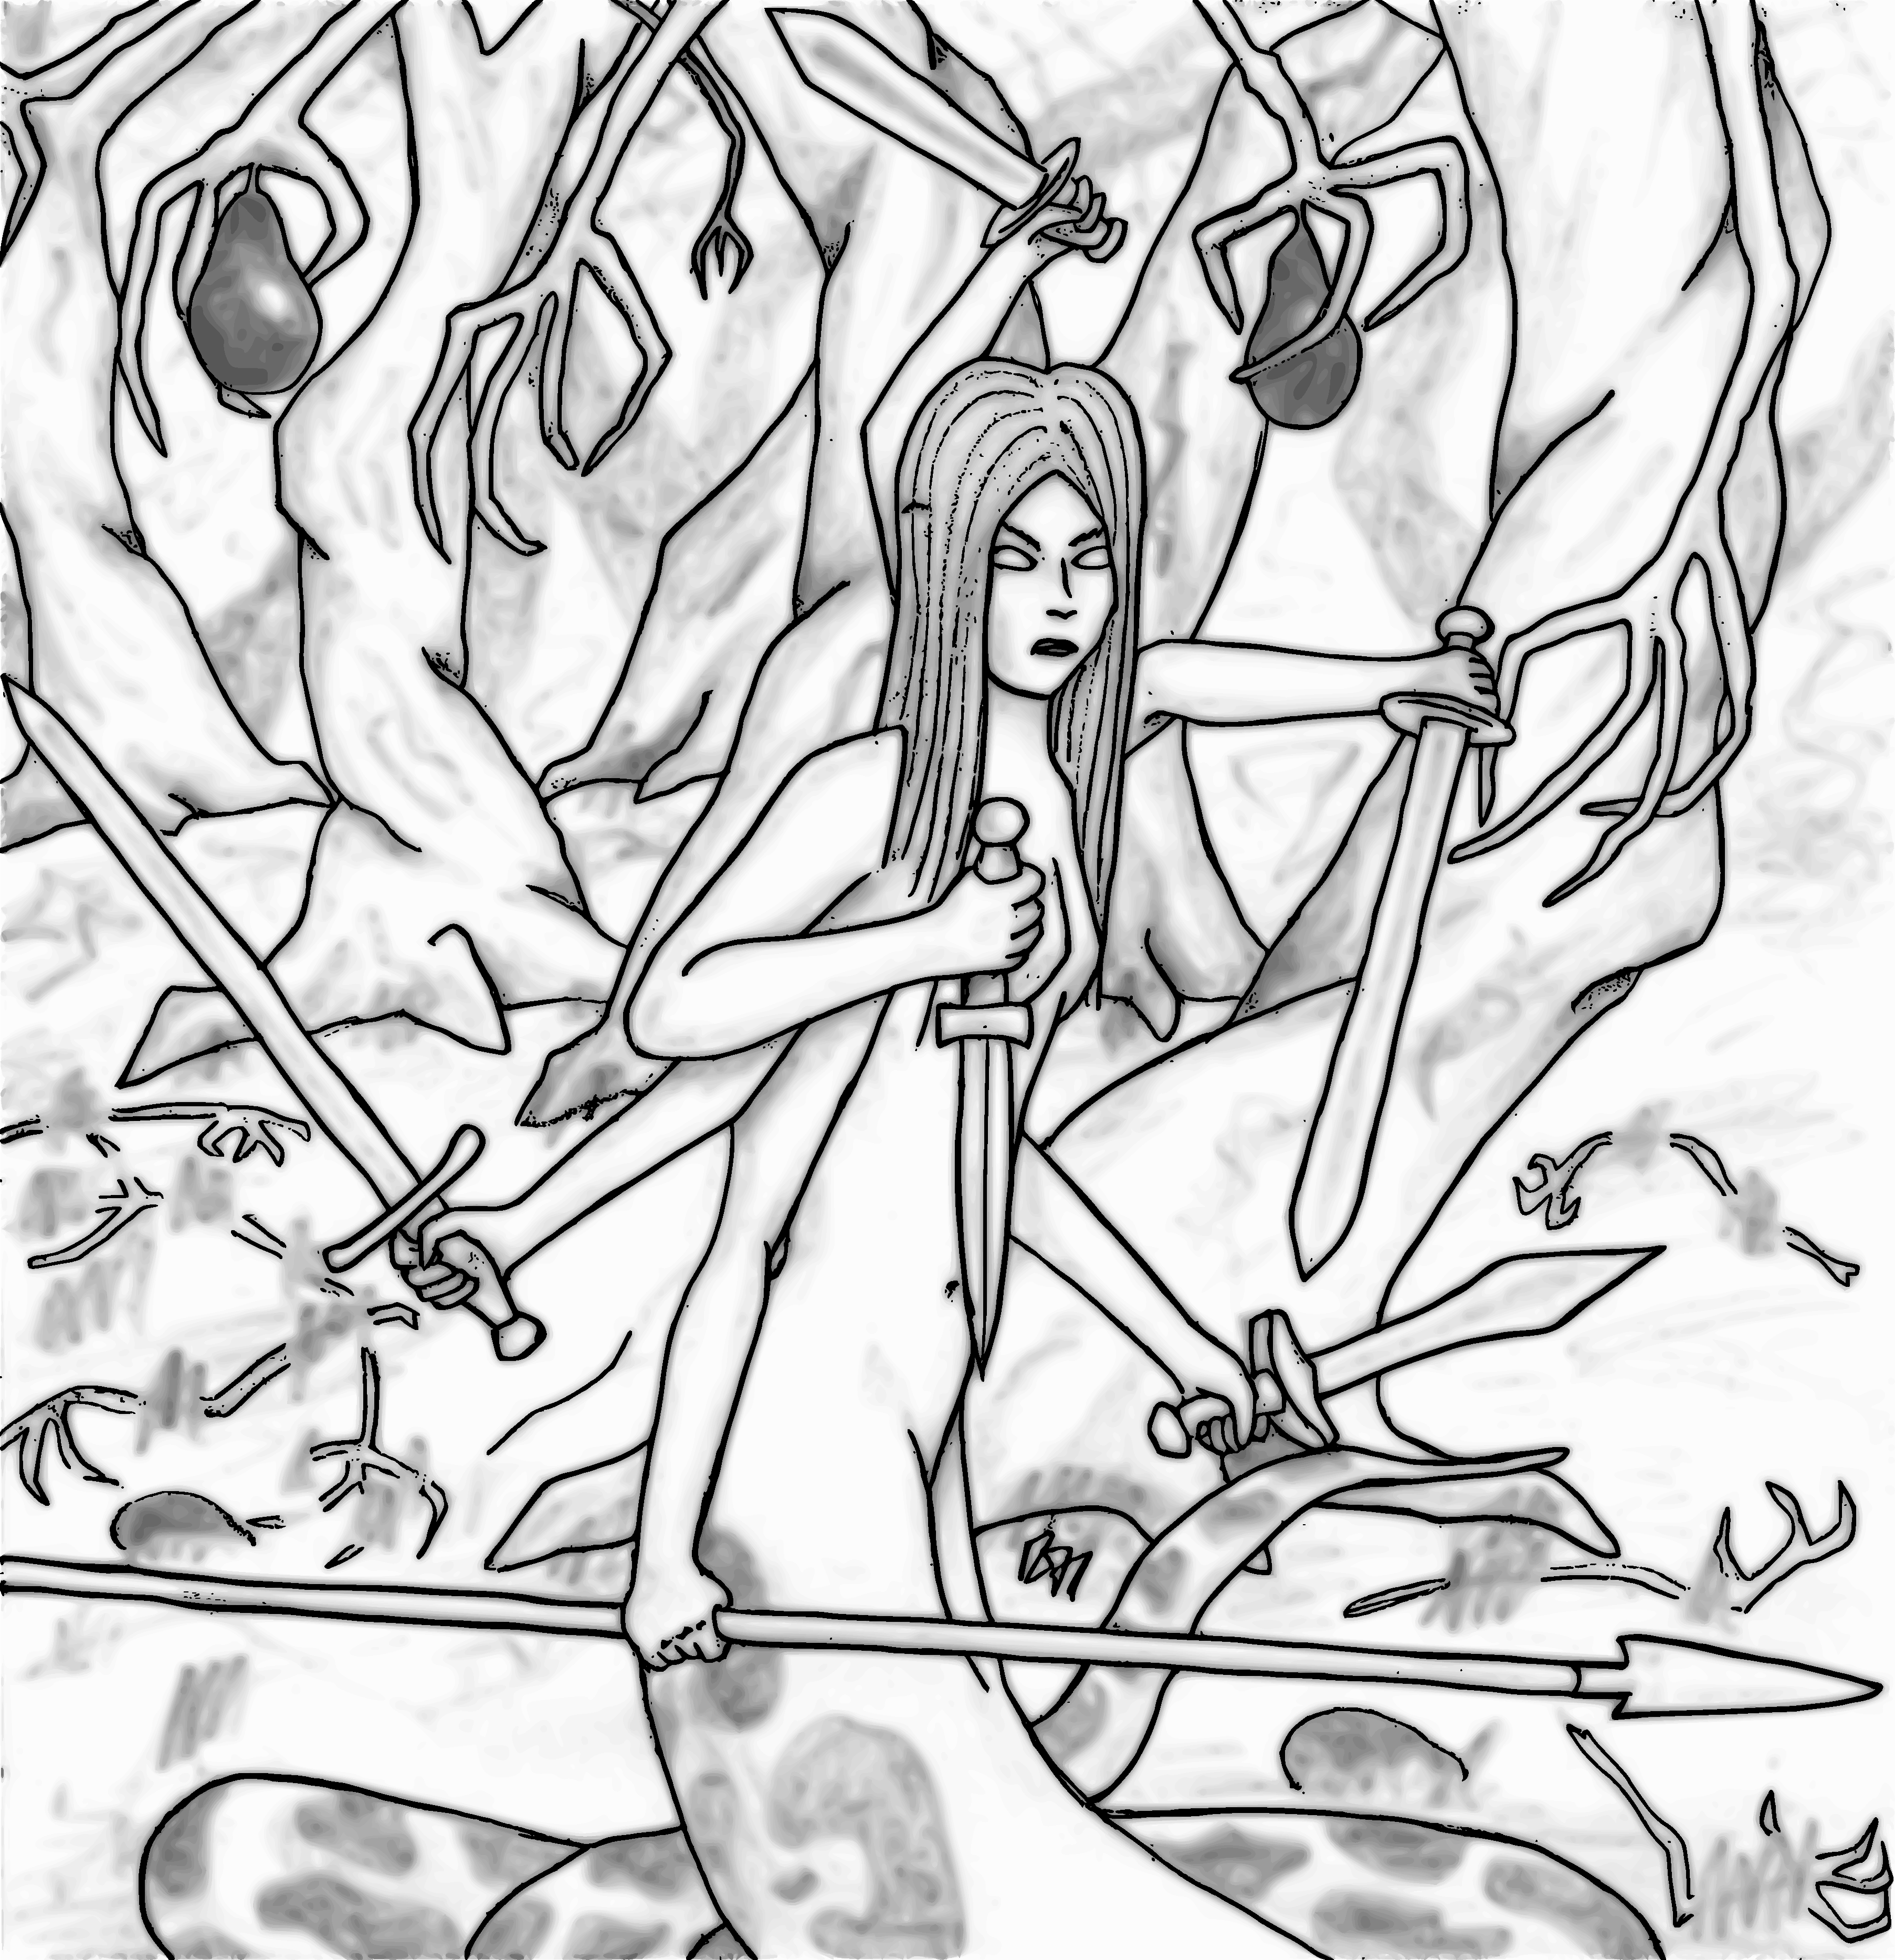
\includegraphics[width=\columnwidth]{marilith.pdf}\label{marilith}

\index{Demon!Marilith}\subsubsection{MARILITH}

Among the most powerful of demons, mariliths are as devious and ruthless as they are terrifying. From the waist up, mariliths have the bodies of coldly beautiful women with six arms, while from the waist down, they have the bodies of snakes. Mariliths can speak any language, but usually communicate telepathically. Mariliths have exceptionally keen senses, and can never be surprised or affected by illusions and mind-altering spells.

Mariliths are the intelligences behind demonic war efforts. Although they are as chaotic as any of their kind, they understand order and its value in war. They serve as generals, directing hordes of lesser demons and bullying them into following their directives. But even so, mariliths are still demons, and enjoy nothing more than giving into their chaotic natures and wading into the thick of battle.

\textbf{Combat:} Mariliths are terrifying combatants. Able to attack with each of their six arms, mariliths arm themselves with the finest weapons available, and are likely to have collected several powerful magical weapons throughout their long lives. Only the youngest mariliths are armed with non-magical weapons.

In addition to her weapons, a marilith can attack with her tail. A marilith who makes a successful tail attack may wrap her tail around her victim. Each round thereafter she may constrict her victim, automatically inflicting 4d6 points of damage. Constricted creatures must make a constitution check each round or fall unconscious. Only the strongest creatures have any hope of breaking free from a marilith's coils; for every point of strength above 14, a creature has a 10\% chance of breaking free.

In addition to the abilities that all demons possess, mariliths can use the following spells at will: \textit{animate dead}, \textit{cause serious wounds}, \textit{cloudkill}, \textit{comprehend languages}, \textit{curse}, \textit{detect evil}, \textit{detect magic}, \textit{detect invisibility}, \textit{polymorph self}, \textit{project image}, \textit{pyrotechnics}, and \textit{telekinesis}. All of these may be used any number of times except for \textit{polymorph self}, which may be used 7 times each day. A marilith may attempt to use \textit{gate} once each hour to summon 2d10 dretches or 1 marilith with a 35\% chance of success.

\noindent \begin{minipage}{\columnwidth}

\vspace{1em}

\index{Devil}\subsection{DEVIL}

\noindent \begin{tabular}{p{.36\columnwidth}g{.24\columnwidth}p{.24\columnwidth}}
							& \textbf{Spigazu}	& \textbf{Pit Fiend}	\\
\textbf{Climate/Terrain:}	& Evil planes	& Evil planes	\\
\textbf{Frequency:} 		& Common	& Very rare	\\
\textbf{Organization:} 		& Solitary	& Solitary	\\
\textbf{Activity Cycle:} 	& Any	& Any	\\
\textbf{Diet:} 				& Carnivore	& Carnivore	\\
\textbf{Intelligence:} 		& 8--12	& 17--18	\\
\textbf{Treasure:} 			& None	& G, W	\\
\textbf{Alignment:} 		& Lawful evil	& Lawful evil	\\
\hline
\textbf{Number Appearing:} 	& 1d4	& 1d2	\\
\textbf{Armor Class:} 		& 4	& $-5$	\\
\textbf{Movement:} 			& 6, fly 18 C	& 15, fly 24 C	\\
\textbf{Hit Dice:} 			& 3 + 3 (16 hp)	& 13 (59 hp)	\\
\textbf{THACO:} 			& 17	& 7	\\
\textbf{Attack:} 			& 2 claws 1d4, by weapon	& 2 wings 1d4, bite 2d6, tail 2d4, (2 claws 1d6 or by weapon + 6) \\
\textbf{Special Traits:} & Attack type immunities, spells, spikes	& Attack type immunities, constriction, disease, fear, poison, regeneration, spells, +3 or better weapon needed to hit	\\
\textbf{Magic Resistance:} 	& 15\%	& 50\%	\\
\textbf{Size:} 				& Small (3' tall)	& Large (12' tall)	\\
\textbf{Morale:} 			& 8--10	& 19--20	\\
\textbf{Experience:} 		& 3,000	& 26,000	\\ % 3,000 & 21,000
\end{tabular}

\end{minipage}

Devils are exemplars of law and evil, the very principle of these ideas made flesh. They have many forms, from the beautiful to corrupt those driven by lust, to the horrid to strike fear into the hearts of even the brave. Each form serves a purpose, and as a devil gains mastery of new responsibilities, it is granted a new form.

Devils are ranked in an elaborate and byzantine hierarchy from the least powerful to the most. Each rank in the hierarchy has its own duties and functions, and a devil that serves these well--or engineers the fall of a superior--may be promoted to the next rank. The duties of the lesser devils are small, perhaps to fight as soldiers or to corrupt mortal souls. But power comes with responsibility, and the duties of the greater devils are likewise greater; for example, to serve as generals and commanders.

Devils are natives of the lawful evil planes, and rarely walk freely upon the Prime Material plane. They readily enter into contracts and bindings with mortal spellcasters, eager to twist the terms of such contracts to their own evil ends. As immortal creatures of malignant order, the devils are rarely bested or outwitted by any mortals who seek to bind them to service.

Despite both races being creatures of primordial evil, devils hold a great hatred of demons. Both sides likely see their ways as the true path of evil, and the ways of the other as weak and corrupt. Regardless of the reason, their hatred of each other manifests as genocidal violence whenever the two races meet.

Devils speak their own infernal tongue, and those smart enough may learn a staggering array of other languages. Devils with intelligence scores of 8 or greater can communicate with other intelligent creatures via telepathy.

\textbf{Combat:} All devils are immune to damage from fire (both normal and magical varieties) and poison, and take only half damage from cold.

\index{Devil!Spigazu}\subsubsection{SPIGAZU}

Spigazu are lesser devils, among the weakest of devil-kind but found in vast numbers. Diminutive and grotesque, spigazu look like twisted humanoids covered in spikes and sporting leathery wings.

Physically weak, spigazu serve better as scouts and messengers than as soldiers. They are intelligent creatures, able to carry out complex instructions and operate under little supervision. Loyal to a point, a spigazu will serve to the best of its ability in hopes of promotion as long as its superior shows no weakness. However, if given a chance, a spigazu will exploit any flaw to betray a superior if it thinks it can gain from the betrayal.

\textbf{Combat:} Spigazu are weak creatures, and prefer to attack from the air when forced into combat. They tend to favor weapons that can be used at range.

A spigazu may launch two of its spikes as missile weapons each round until all twelve are exhausted. Once launched, the spikes burst into flame, and may ignite flammable material on contact. A spigazu's spikes have a short range of out to 30', medium range out to 60', and long range out to 120', and inflict 1d3 points of damage on a successful hit. Spikes spent in this manner are regrown after a week's growth. A spigazu may instead hurl itself bodily at a foe to wound it with 1d4 spikes. The spikes are not lost in this case, but a spigazu can take no other attacks that round.

A spigazu may use the spells \textit{affect normal fires}, \textit{change self}, \textit{command}, \textit{produce flame}, \textit{scare}, and \textit{stinking cloud} at will. Once each day, it may attempt to use \textit{gate} to summon 1d3 fellow spigazu with a 35\% chance of success.

\index{Devil!Pit Fiend}\subsubsection{PIT FIEND}

Pit fiends are the greatest of all devils and the undisputed masters of their kind. They appear as hulking humanoids looming twice as large as a man, with cloak-like wings and huge dripping fangs.

Pit fiends are the royalty of devil-kind, having attained their ranks after millennia of loyal and flawless service during their time as lesser devils. Wielding unimaginable power, their decisions determine the policies of all of devil-kind. Pit fiends are driving force behind the devils' war against the demons, serving as generals of vast armies and bringing their impressive strength and magic into the thick of battle.

\textbf{Combat:} Pit fiends are terrifying foes, capable of fighting off legions of lesser beings by themselves. A pit fiend may attack with a weapon, almost certainly magical and wielded with an impressive strength of 18/00 (+6 damage). Lacking a weapon, a pit fiend may use its two claws to great effect. Armed or not, a pit fiend can attack with its wings, its toxic bite, and its tail. Victims bitten are poisoned and, failing a save vs. poison, die within 1d4 rounds. Even those that survive are infected with a terrible disease.

If a pit fiend hits with its tail attack, it may constrict its victim and automatically deal 2d4 points of damage each round thereafter until a victim makes a successful strength check to break free.

In addition to their fearsome attacks, pit fiends regenerate 2 hit points each round, and radiate \textit{fear}  within a 20' radius.

A pit fiend may use the following spells at will: \textit{advanced illusion}, \textit{animate dead}, \textit{charm person}, \textit{detect magic}, \textit{detect invisibility}, \textit{fireball}, \textit{hold person}, \textit{improved invisibility}, \textit{infravision}, \textit{know alignment}, \textit{polymorph self}, \textit{produce flame}, \textit{pyrotechnics}, \textit{suggestion}, \textit{teleport without error}, and \textit{wall of fire}. A pit fiend may call upon its stronger magics and use \textit{symbol} (of pain) once per day and cast \textit{wish} once each year. A pit fiend may use \textit{gate} once each round to summon four spigazu or one fellow pit fiend.

\index{Dragon}\subsection{DRAGON}

Dragons are ancient and magical reptilian creatures. No mere animals, dragons are as far beyond normal reptiles as humans are lesser mammals. They are breathtaking creatures, with huge wings, serpentine bodies, and armor-like scales. Different races of dragons are distinguishable by the color of their scales, which shine like metal on the noble and good and burn with primal color for the evil.

Dragons are known for their intelligence, which can range from the low cunning of the weakest and youngest dragons to the boundless genius of the greatest and oldest wyrms. Most dragons can speak; dragons speak the dialect of their own kind and usually speak the high form of dragonspeak from which all dialects are derived. Wiser and more curious dragons may speak any language that suits their needs. Even the best dragons tend to be greedy, and all but the youngest collect great hordes of treasure. Some sages theorize that these treasures are essential for a dragon to grow. Although most dismiss this idea, dragons guard their treasure as they guard their own lives, and go to great lengths to recover lost or stolen treasure.

As powerful and greedy beings, dragons are usually solitary creatures. Occasionally, a dragon will take a mate and raise a brood of hatchlings, although most of these families dissolve once the young are grown. Dragons tend to be attentive parents and protect their young until they are able to fend for themselves, although different varieties of dragons have different ideas of when their offspring can do so.

Like all living creatures, dragons grow in size and power with age, but great age does not bring weakness and decrepitude to dragons as it does others. From the moment they hatch, dragons grow in power, knowledge, and might, and the eldest are the mightiest of their race.

A dragon's power increases with age. The descriptions and statistics given for each dragon type are for young adults, those who have left their parents behind and have begun to establish themselves on their own. The statistics for younger and older dragons can be determined by Table \ref{dragonages}: Dragon Age Categories and Modifiers. Adjust the statistics given by the chosen dragon type's description by the modifiers given by the table for the chosen age category.

\subsubsection*{Age Categories} 

As dragons grow in age and size, they also learn and develop magic, skills, and other abilities. Although each dragon is unique and grows at a different rate than other dragons, age categories are a somewhat inexact way of determining how much a dragon has grown in size and power. Approximate age ranges for each age category are given.

\paragraph{Treasure:} A dragon begins to accumulate a horde after leaving the care of its parents. As it grows, so too does its horde.

\paragraph{Armor Class:} A dragon's scales start out relatively thin and weak, but grow to rival metal and stone as the dragon ages.

\paragraph{Hit Dice:} As a dragon's size increases, so does its ability to withstand damage.

\paragraph{THACO:} Like other creatures, a dragon's THACO is dependent on its hit dice. Older and larger dragons are more effective in combat than younger and smaller dragons.

\paragraph{Damage Modifier:} A dragon's musculature grows alongside its size, and larger dragons are capable of inflicting more damage with physical attacks.

\paragraph{Breath Weapon Damage:} A dragon learns to channel more and more energy into its breath weapon as it ages. Although the  dice used to determine the damage is different for each variety of dragon, the number of dice used is the same for all dragons of a given age category. For example, juvenile dragons inflict 8d\textit{x} + 5 points of damage with their breath weapons---white dragons use a d3 to determine breath weapon damage so a juvenile white dragon's breath inflicts 8d3 + 5 of damage, while bronze dragons use a d8 to determine breath weapon damage so a young adult bronze dragon's breath inflicts 8d8 + 5 points of damage.

A dragon's breath weapon automatically hits all creatures caught within its area of effect, but a creature may save vs. breath weapon to take half damage.

\paragraph{Magic Resistance:} After growing to a certain size, dragons become resistant to magic. Older dragons are able to shrug off magic that would affect a younger dragon.

\paragraph{Size:} A dragon's size increases as it gets older. The size listed in a dragon's description is the size of its body; its tail is of a comparable size.

\end{multicols}

\noindent \begin{minipage}{\columnwidth}

\captionof{table}{Dragon Age Categories and Modifiers}\label{dragonages}
\noindent \begin{tabular}{|p{.15\columnwidth}|p{.1\columnwidth}|p{.055\columnwidth}|p{.055\columnwidth}|p{.055\columnwidth}|p{.055\columnwidth}|p{.115\columnwidth}|p{.06\columnwidth}|p{.055\columnwidth}|p{.065\columnwidth}|}
\hline
Age Category	& Treasure	& AC	& HD	& THACO	& Dmg. Mod.	& Breath Weap\-on Damage	& Magic Resist.	& Size	& XP	\\
\hline\hline
\rowcolor[gray]{.9}1: Hatchling (0--5 years)	& None	& +4	& $-7$	& +7	& $-4$	& 2d\textit{x} + 1	& None	& $-90$\%	& $-15,000$	\\
2: Very Young (6--15 years)	& None	& +3	& $-5$	& +5	& $-3$	& 4d\textit{x} + 2	& None	& $-70$\%	& $-13,000$	\\
\rowcolor[gray]{.9}3: Young (16--25 years)		& None	& +2	& $-3$	& +3	& $-2$	& 6d\textit{x} + 3	& None	& $-50$\%	& $-10,000$	\\
4: Juvenile (26--50 years)	& $^1$/$_2$ $\times$ lair, 1 $\times$ indiv.	& +1	& $-1$	& +1	& $-1$	& 8d\textit{x} + 4	& None	& $-25$\%	& $-7,000$	\\
\rowcolor[gray]{.9}5: Young Adult (51--100 years)	& 1 $\times$ lair, 1 $\times$ indiv.	& No adj.	& No adj.	& No adj.	& No adj.	& 10d\textit{x} + 5	& +0\%	& No adj.	& No adj.	\\
6: Adult (101--200 years)	& 1 $\times$ lair, 1 $\times$ indiv.	& $-1$	& +1	& $-1$	& +1	& 12d\textit{x} + 6	& +5\%	& +25\%	& +1,000	\\
\rowcolor[gray]{.9}7: Mature Adult (201--400 years)	& 1 $\times$ lair, 1 $\times$ indiv.	& $-2$	& +2	& $-2$	& +2	& 14d\textit{x} + 7	& +10\%	& +55\%	& +2,000	\\
8: Old (401--600 years)	& 1 $\times$ lair, 2 $\times$ indiv.	& $-3$	& +3	& $-3$	& +3	& 16d\textit{x} + 8	& +15\%	& +85\%	& +3,000	\\
\rowcolor[gray]{.9}9: Very Old (601--800 years)	& 1 $\times$ lair, 2 $\times$ indiv.	& $-4$	& +4	& $-4$	& +4	& 18d\textit{x} + 9	& +20\%	& +120\%	& +4,000	\\
10: Venerable (801--1,000 years)	& 1 $\times$ lair, 2 $\times$ indiv.	& $-5$	& +5	& $-5$	& +5	& 20d\textit{x} + 10	& +25\%	& +150\%	& +5,000	\\
\rowcolor[gray]{.9}11: Wyrm (1,001--1,200 years)	& 1 $\times$ lair, 3 $\times$ indiv.	& $-6$	& +6	& $-6$	& +6	& 22d\textit{x} + 11	& +30\%	& +180\%	& +6,000	\\
12: Great Wyrm (1,201+ years)	& 1 $\times$ lair, 3 $\times$ indiv.	& $-7$	& +7	& $-7$	& +7	& 24d\textit{x} + 12	& +35\%	& +220\%	& +7,000	\\
\hline
\end{tabular}

\end{minipage}

\begin{multicols}{2}



\paragraph{Experience:} Older dragons are more capable and thus more dangerous than younger dragons. A party that defeats an ancient dragon earns more experience than one that defeats a hatchling.

\noindent \begin{minipage}{\columnwidth}

\captionof{table}{Dragon Fear}\label{dragonfear}
\noindent \begin{tabular}{|p{.25\columnwidth}|p{.2\columnwidth}|p{.4\columnwidth}|}
\hline
Age Category	& Fear Radius	& Saving Throw Modifier	\\
\hline\hline
\rowcolor[gray]{.9}Hatchling	& None	& --	\\
Very Young	& None	& --	\\
\rowcolor[gray]{.9}Young		& None	& --	\\
Juvenile	& None	& --	\\
\rowcolor[gray]{.9}Young Adult	& 45'		& +3	\\
Adult		& 60'		& +2	\\
\rowcolor[gray]{.9}Mature Adult	& 75'		& +1	\\
Old			& 90'		& No adj.	\\
\rowcolor[gray]{.9}Very Old	& 105'	& $-1$	\\
Venerable	& 120'	& $-2$	\\
\rowcolor[gray]{.9}Wyrm		& 135'	& $-3$	\\
Great Wyrm	& 150'	& $-4$	\\
\hline
\end{tabular}

\end{minipage}

\subsubsection*{Dragon Fear}

Dragons are terrifying creatures, so much so that the very sight of a dragon can instill terror in even the stoutest of hearts. Creatures with less than 1 HD flee in panic for 4d6 rounds at the sight of a dragon of young adult age or older. Creatures with 1 HD or more but less than the HD of the dragon in question must save vs. petrification when at or closer to the radius indicated by the dragon's age category or fall under the dragon's fear and suffer a $-2$ penalty to all attack and damage rolls. Larger dragons, being more fearsome than smaller dragons, affect a larger radius with their fear.

A dragon's age and size also determines the intensity of its aura of fear. While younger dragons are terrifying in their own right, an elder dragon is much more so. Apply the saving throw modifier for the age category of a dragon to saves vs. the dragon's fear.

\subsubsection*{Attack Forms}

Regardless of age, all dragons are capable of attacking each round with two claws and a bite, and attacking once every three rounds with their breath weapon. A dragon attacking with its claws must attack a target to its front or sides, but may also attack creatures behind them with their bite. A dragon attacking a creature behind it with a rear claw may also attempt to knock its victim back. A victim struck with a rear claw must successfully make a dexterity check or be knocked back 1d6 feet plus 1 foot per age category of the dragon and make a successful save vs. petrification or be knocked prone. Regardless of which claws it uses, a dragon may not attack with more than two of its claws.

A dragon of young adult age or older may attack foes at its flanks by buffeting them with its wings. A wing buffet inflicts damage equal to a claw attack, and a buffeted creature must make a successful dexterity check or be knocked prone.

A dragon of young adult age or older may snatch up a creature of two or more size categories smaller with a successful talon attack; large creatures can be snatched up if both talon attacks succeed. Caught victims are 50\% likely to have their arms pinned. A dragon may transfer a caught victim to his mouth with a successful bite attack; if this attack fails, the caught victim is dropped. Each round, a dragon may squeeze or bite caught victims held in his claw or mouth to inflict damage equal to a claw or bite attack, respectively. A dragon of old age or older may snatch up a creature in each claw, and a wyrm or great wyrm may carry a victims in his mouth and both claws at once. Caught victims may break free with a successful strength---bend bars/lift portcullis check. 

A dragon of adult age or older may sweep foes to its rear or flank with its tail. A tail sweep may target as many foes as a dragon's age category, and a separate attack roll must be made against each foe. A successful tail sweep inflicts damage equal to two claw attacks, and a swept creature must save vs. petrification or be stunned for 1d4 + 1 minutes. A dragon's tail sweep also does siege damage to structures as per a battering ram.

\subsubsection*{Spells}

Dragons are curious and have a natural aptitude for magic. Through exploration and study, a dragon learns spells as it ages, but dragons do not use magic like humanoids do. Dragons do not study spellbooks or pray to gods for their spells, but they only know a set number of spells and cannot choose to cast different spells another day. A dragon may cast each spell it knows once per day, and needs only sleep to regain its spells. Spells cast by a dragon do not require somatic or material components and have a casting time of 1, but cannot be used in the same round a dragon attacks or uses its breath weapon.

Dragons cast spells equivalent to spellcasters of the level given by their specific type description plus the damage modifier for their age category.

\end{multicols}

\pagebreak

\noindent \begin{minipage}{\columnwidth}

\index{Dragon!Chromatic}\subsection*{DRAGON, CHROMATIC}

\noindent \begin{tabular}{p{.20\columnwidth}g{.13\columnwidth}p{.13\columnwidth}g{.13\columnwidth}p{.13\columnwidth}g{.13\columnwidth}}
				& \textbf{Black Dragon}	& \textbf{Blue Dragon}	& \textbf{Green Dragon}	& \textbf{Red Dragon}	& \textbf{White Dragon}	\\
\textbf{Climate/Terrain:}	& Any wetlands		& Any deserts		& Any forests and jungles	& Any hills and mountains	& Any arctic	\\
\textbf{Frequency:} 		& Rare			& Very rare		& Very rare		& Very rare		& Rare	\\
\textbf{Organization:} 		& Solitary or clan	& Solitary or clan	& Solitary or clan	& Solitary or clan	& Solitary or clan	\\
\textbf{Activity Cycle:} 	& Any			& Any			& Any			& Any			& Any	\\
\textbf{Diet:} 			& Carnivore		& Carnivore		& Carnivore		& Carnivore		& Carnivore	\\
\textbf{Intelligence:} 		& 8--10			& 11--12		& 11--12		& 15--16		& 5--7	\\
\textbf{Treasure:} 		& H	& H, (S)	& H			& H, (S), (T)	& E, (O), (S)	\\
\textbf{Alignment:} 		& Chaotic evil		& Lawful evil		& Lawful evil		& Chaotic evil		& Chaotic evil	\\
\hline
\textbf{Number Appearing:} 	& 1 or 1d4 + 1		& 1 or 1d4 + 1		& 1 or 1d4 + 1		& 1 or 1d4 + 1		& 1 or 1d4 + 1	\\
\textbf{Armor Class:} 		& 0			& $-1$			& $-1$			& $-4$			& 0	\\
\textbf{Movement:} 		& 12, fly 30 C, swim 12	& 9, fly 30 C, burrow 4	& 9, fly 30 C, swim 9	& 9, fly 30 C		& 12, fly 40 C, swim 12, burrow 6	\\
\textbf{Hit Dice:} 		& 13 (59 hp)		& 15 (68 hp)		& 14 (63 hp)		& 16 (72 hp)		& 12 (54 hp)	\\
\textbf{THACO:} 			& 	8						& 6						& 	7						& 	5						& 	9					\\
\textbf{Attack:} 		& 2 claws 1d6 + 5, bite 3d6 + 5	& 2 claws 1d8 + 5, bite 3d8 + 5	& 2 claws 1d8 + 5, bite 2d10 + 5	& 2 claws 1d10 + 5, bite 3d10 + 5	& 2 claws 1d6 + 5, bite 2d8 + 5	\\
\textbf{Special Traits:} 	& Acid immunity, breath weapon, spells	& Breath weapon, electricity immunity, spells	& Breath weapon, poison immunity, spells	& Breath weapon, fire immunity, spells	& Breath weapon, cold immunity, spells	\\
\textbf{Magic Resistance:} 	& 10\%			& 20\%		 	& 15\%			& 30\%			& 5\%	\\
\textbf{Size:} 			& Gigantic (40' long)	& Gigantic (56' long)	& Gigantic (48' long)	& Gigantic (64' long)	& Gigantic (32' long)	\\ %134% of MM value
\textbf{Morale:} 		& 17--18		& 17--18		& 15--16		& 17--18		& 15--16	\\
\textbf{Experience:} 		& 18,000		& 20,000		& 20,000		& 23,000		& 16,000	\\
\end{tabular}

\end{minipage}

\begin{multicols}{2}

\index{Dragon!Chromatic!Black}\subsubsection{BLACK DRAGON}

Black dragons are hatched with small, shiny black scales, but these grow thicker and less glossy with age, reaching a dull matte appearance by adulthood. A black dragon has two horns jutting forward from its temples, and a webbed fin running the length of its neck. All black dragons can breathe water as easily as they can air.

Sneaky, foul-tempered, and secretive, black dragons shun other creatures. They only rarely take mates, and even then often choose to lair alone. They prefer to dwell in swamps, rain forests, and other wet and dark places and often make their lairs underwater.

Like all dragons, black dragons are carnivores, and prefer to eat fish, crustaceans, and other aquatic animals. When they catch land animals, they often let it ``steep" in a stagnant swamp for days before eating it.

\textbf{Combat:} Black dragons prefer to trap and ambush their foes and use their surroundings and abilities to their fullest advantage. They rarely rush carelessly into battle, and often spend long amounts of time hiding from and sizing up their foes before attacking.

A black dragon's breath weapon is a stream of acid 5' wide and stretching as far as 60' long. The damage inflicted by this breath weapon is determined using d4s. 

Black dragons are relatively weak spellcasters, equivalent to 5\textsuperscript{th} level. A juvenile black dragon learns 1 1\textsuperscript{st} level wizard spell, and learns 1 additional 1\textsuperscript{st} level wizard spell each age category thereafter. 

In addition to spells learned, juvenile and older black dragons gain the use of the \textit{darkness} spell 3 times each day with an effective radius of 10' per age category. Adult and older black dragons may use \textit{putrefy food \& drink} once each day to affect 10 cubic feet of water per age category. Old and older black dragons may use \textit{plant growth} once each day, and venerable and older black dragons may use \textit{summon insects} once each day. Great wyrm black dragons may charm reptiles (and reptiles only) 3 times each day as per the \textit{charm monster} spell.

\index{Dragon!Chromatic!Blue}\subsubsection{BLUE DRAGON}

Blue dragons have a pair of back-sweeping horns growing from their temples and a row of horns running the length of their snouts. The horn at the end of a blue dragon's snout often grows to prodigious size. Their polished scales range in color from light azure to deep midnight blue, although both extremes are rare.

Blue dragons tend to be aloof from other creatures, and are extremely covetous of their territory and possessions. They spend great amounts of time flying over their lands, enjoying the sight of their domains as well as patrolling for intruders. They prefer to live in deserts, badlands, and other hot and arid places.

Unusually, blue dragons are able to eat plants in addition to meat when food is scarce, although they do not particularly enjoy them.

\textbf{Combat:} Blue dragons are adept at attacking from the air, preferring to soar high above their foes and remain out of range of retribution. They hate to back down from a fight, and tend to do so only do so when severely overmatched.

A blue dragon's breath weapon is a stroke of lightning 5' wide and up to 100' long. The damage inflicted by this breath weapon is determined using d8s. 

Blue dragons are adept at spell use, casting spells as 7\textsuperscript{th} level casters. A juvenile blue dragon learns to cast 1 1\textsuperscript{st} level wizard spell, and learns 1 additional spell at each additional age category. These spells may include 2\textsuperscript{nd} level spells starting upon the dragon reaching mature adult age, and may include 3\textsuperscript{rd} level spells starting upon the dragon reaching venerable age. Further, a venerable blue dragon learns to cast 1 1\textsuperscript{st} level priest spell, and learns an additional 1\textsuperscript{st} level priest spell at each age category thereafter.

In addition to learned spells, young blue dragons gain the ability to cast \textit{create water} and \textit{destroy water} 3 times each day. Adult and older blue dragons can cast \textit{dust devil} once each day, old and older blue dragons can cast \textit{ventriloquism} once each day, venerable and older blue dragons can cast \textit{control winds} once each day, and great blue wyrms can cast \textit{hallucinatory terrain} once each day.

\index{Dragon!Chromatic!Green}\subsubsection{GREEN DRAGON}

Green dragons hatch with delicate, dark green scales which thicken and lighten as they grow. A green dragon is readily identifiable by the fin-like crest that runs the length of its spine, from its skull to the tip of its tail.

Green dragons are cruel and sadistic creatures that take delight in the suffering of those they deem to be lesser creatures (almost everything). They suffer no competition to their rule, and will kill or drive away from their domains any creatures that they cannot enslave. Despite their hatred of other creatures, green dragons are found in family groups more often than other dragons. They are devoted parents, and cooperate in raising and protecting their young together.  Green dragons like to make their lairs in impenetrable thickets deep in the hearts of primeval forests, but will settle for most forested areas.

\textbf{Combat:} Green dragons are vicious and fearless, and will not hesitate to attack creatures that they deem threatening. Unless they are obviously outmatched, they show little concern for the power of their foes.

A green dragon's breath weapon is a cloud of poisonous gas, billowing out to 50' long, 40' wide, and 30' tall. The damage inflicted by this breath weapon is determined using d6s. 

Green dragons are capable spellcasters, and cast spells as if they were 6\textsuperscript{th} level. Starting at the juvenile age category, green dragons may learn 1 wizard spell each time they advance an age category. These start out as 1\textsuperscript{st} level wizard spells, but old and older dragons may learn 2\textsuperscript{nd} level wizard spells as well.

In addition to their learned spells, all blue dragons gain certain spells as they age. Juvenile and older dragons can cast \textit{water breathing} once each day, adult and older dragons can cast \textit{suggestion} once each day, mature adults and older dragons can cast \textit{warp wood} 3 times each day, old and older dragons can cast \textit{plant growth} once each day, very old and older dragons can cast \textit{entangle} once each day, and green wyrms and great wyrms can cast \textit{pass without trace} 3 times a day.

\index{Dragon!Chromatic!Red}\subsubsection{RED DRAGON}

At hatching, a red dragon's scales are glossy and brilliantly colored, but they grow more subdued and dull as the dragon ages. Red dragons are crowned by distinctive horns and spines.

Red dragons are the greatest of the chromatic dragons. They are egotistical, vain, and convinced of their superiority over all others. Covetous of both wealth and territory, red dragons seek to gain both and jealously guard the treasure and land they already have. They have a weakness for flattery, and may grant creature which entertain their vanity their lives---at least until they grow bored. Due to their greedy and territorial natures, red dragons rarely live with others of their kind. Their lairs---often located in winding caverns or atop soaring mountains--are their own, and even families are loathe to share the same lair.

\textbf{Combat:} Convinced of their superiority and might, red dragons rarely consider a foe's capabilities before committing themselves to combat. Due to their overwhelming might, such shortsightedness is rarely to a red dragon's detriment.

A red dragon's breath weapon is a cone-shaped gout of fire 5' wide at the base and 30' wide at its full length of 90'. The damage inflicted by this breath weapon is determined using d10s. 

Red dragons are very adept at magic and cast spells as if they were 9\textsuperscript{th} level. Red dragons learn one wizard spell at the juvenile age category and at each age category thereafter. Dragons younger than adult age may only learn 1\textsuperscript{st} level spells, while dragons older than young adult age may learn 2\textsuperscript{nd} level wizard spells, dragons older than mature adult age may learn 3\textsuperscript{rd} level wizard spells, dragons older than very old age may learn 4\textsuperscript{th} level wizard spells, and great wyrms may learn a 5\textsuperscript{th} level wizard spell. Red dragons of venerable age learn one priest spell each age category. Venerable dragons and wyrms may only learn 1\textsuperscript{st} level priest spells, while great wyrms may learn one 2\textsuperscript{nd} level priest spell.

In addition to their learned spells, all red dragons of young age or older can cast \textit{affect normal fires} three times each day. Red dragons of juvenile age or older can cast \textit{pyrotechnics} three times each day, dragons of adult age or older can cast \textit{heat metal} once each day, dragons of old age or older may cast \textit{suggestion} once each day, and dragons of very old age or older may cast \textit{hypnotism} once each day.

\index{Dragon!Chromatic!White}\subsubsection{WHITE DRAGON}

The smallest of the chromatic dragons, white dragons have pure white mirror-like scales at birth, which darken and dull to white mixed with gray and blue as the dragons age. White dragons have a characteristic bony crest on the back of their heads.

White dragons are less intelligent than other dragons, and are often bestial and brutish. They live to hunt, collect treasure, and mate, and do not often care about other concerns. White dragons are sometimes found together as families. These families are not close, and the family members tolerate each other rather than form closer bonds. Young dragons are left to fend for themselves at an early age, but even the youngest are more than capable of the task. White dragons live wherever they can find suitably cold lairs, and prefer glacial caves to nest in. 

\textbf{Combat:} White dragons do not employ much strategy or thought when fighting. They attack by instinct and throw their might at their largest threat, and readily flee if they feel that they are likely to be defeated.

A white dragon's breath weapon is a cone of icy air and sleet 70' long, starting at 5' wide at its base and expanding to 25' wide at the far end. Damage inflicted by this breath weapon is determined using d3s.

Despite the draconic affinity for magic, white dragons are weak spellcasters, and cast spells at 5\textsuperscript{th} level. white dragons learn one 1\textsuperscript{st} level wizard spell each at their adult, old, venerable, and great wyrm age categories.

In addition to their learned spells, white dragons of mature adult age or older can cast \textit{gust of wind} three times each day. Dragons of very old age or older can cast \textit{wall of fog} three times each day, and dragons of wyrm age or older can cast \textit{freezing sphere} three times each day.

\end{multicols}

\noindent
\includegraphics[width=\columnwidth, height=2.75in]{testblock.pdf}

\noindent \begin{minipage}{\columnwidth}

\index{Dragon!Metallic}\subsection*{DRAGON, METALLIC}

\noindent \begin{tabular}{p{.18\columnwidth}g{.13\columnwidth}p{.14\columnwidth}g{.14\columnwidth}p{.13\columnwidth}g{.13\columnwidth}}
				& \textbf{Brass Dragon}	& \textbf{Bronze Dragon}	& \textbf{Copper Dragon}	& \textbf{Gold Dragon}	& \textbf{Silver Dragon}	\\
\textbf{Climate/Terrain:}	& Any desert or plains		& Any lake or sea shore		& Any hills or mountains		& Any		& Any mountains		\\
\textbf{Frequency:} 		& Rare		& Very rare		& Rare		& Very rare		& Very rare		\\
\textbf{Organization:} 		& Solitary or clan	& Solitary or clan	& Solitary or clan	& Solitary or clan	& Solitary or clan	\\
\textbf{Activity Cycle:} 	& Any			& Any			& Any			& Any			& Any	\\
\textbf{Diet:} 				& Carnivore		& Carnivore		& Carnivore		& Carnivore		& Carnivore	\\
\textbf{Intelligence:} 		& 13--14		& 15--16		& 13--14		& 17--18		& 15--16		\\
\textbf{Treasure:} 			& H		& H, (S), (T)		& H, (S)		& H, (R), (T)		& H, (R)		\\
\textbf{Alignment:} 		& Chaotic good		& Lawful good		& Chaotic good		& Lawful good		& Lawful good		\\
\hline
\textbf{Number Appearing:} 	& 1 or 1d4 + 1		& 1 or 1d4 + 1		& 1 or 1d4 + 1		& 1 or 1d4 + 1		& 1 or 1d4 + 1	\\
\textbf{Armor Class:} 		& $-1$		& $-3$		& $-2$		& $-5$		& $-4$		\\
\textbf{Movement:} 			& 12, fly 30 C, burrow 6		& 9, fly 30 C, swim 12		& 9, fly 30 C		& 12, fly 40 C, swim 12		& 9, fly 30 C		\\
\textbf{Hit Dice:} 			& 13 (59 hp)		& 15 (68 hp)		& 14 (63 hp)		& 17 (77 hp)		& 16 (72 hp)		\\
\textbf{THACO:} 			& 8		& 6		& 7		& 4		& 5		\\
\textbf{Attack:} 			& 2 claws 1d6 + 5, bite 4d4 + 5	& 2 claws 1d8 + 5, bite 4d6 + 5	& 2 claws 1d6 + 5, bite 5d4 + 5	& 2 claws 1d10 + 5, bite 6d6 + 5	& 2 claws 1d8 + 5, bite 5d6 + 5	\\
\textbf{Special Traits:} 	& Breath weapons, fire immunity, spells	& Breath weapons, electricity immunity, spells	& Acid immunity, breath weapons, spells	& Breath weapons, fire and poison immunity, spells	& Breath weapons, cold immunity, spells	\\
\textbf{Magic Resistance:} 	& 15\%		& 20\%		& 10\%		& 35\%		& 25\%		\\
\textbf{Size:} 				& Gigantic (40' long)		& Gigantic (56' long)		& Gigantic (48' long)		& Gigantic (72' long)		& Gigantic (64' long)		\\ %134% of MM value
\textbf{Morale:} 			& 17		& 17		& 16		& 17--18		& 17--18		\\
\textbf{Experience:} 		& 19,000		& 22,000		& 21,000		& 24,000		& 23,000		\\
\end{tabular}

\end{minipage}

\begin{multicols}{2}

\index{Dragon!Metallic!Brass}\subsubsection{BRASS DRAGON}

Brass dragons hatch with thin, brown scales, which thicken and turn to a warm, polished brass color as the dragons age. They have prominent ridges at the back of their heads, distinguishing them from other metallic dragons which may be similar in color.

Brass dragons are friendly and social creatures. Although they usually live alone, they enjoy the company of others and often travel to visit with other dragons. They form close families which stay in contact with each other even if they have dispersed to their own territories. Parents dote on their hatchlings and young, and go to great lengths to protect them.

Brass dragons prefer to live in deserts or other arid environments, and often choose lairs that have views of scenic surroundings. As they prefer to live in the same kinds of areas as blue dragons, they often come into conflict with their larger cousins.

\textbf{Combat:} Brass dragons dislike fighting and prefer to talk and negotiate their ways out of conflict. If combat is inevitable, a brass dragon fights fiercely and uses its abilities to their full advantage to end the fight quickly.

Brass dragons have two breath weapons. The first is a cone-shaped blast of superheated air and stinging sand, 5' wide at the base, 70' long, and 20' wide at the far end. Damage inflicted by this breath weapon is determined using d4s. Alternatively, a brass dragon may breathe a cloud of sleep gas 50' long, 40' wide, and 20' high. Creatures caught within the cloud must save vs. dragon breath or fall asleep for 10 minutes per age category of the dragon.

Brass dragons are capable spellcasters, and cast spells at 6\textsuperscript{th} level. They learn one 1\textsuperscript{st} level wizard spell at juvenile age, and learn either a 1\textsuperscript{st} level or 2\textsuperscript{nd} level wizard spell at each subsequent age category. Brass dragons also learn one 1\textsuperscript{st} level priest spell at old age and learn either a 1\textsuperscript{st} level or 2\textsuperscript{nd} level priest spell at each subsequent age category. A brass dragon may never learn more 2\textsuperscript{nd} level spells of either kind than 1\textsuperscript{st} level spells.

In addition to learned spells, brass dragons of juvenile age or older can cast \textit{dust devil} once each day, dragons of adult age or older can cast \textit{suggestion} once each day, dragons of mature adult age or older can control the temperature of its surroundings as per the \textit{control temperature 10' radius} spell 3 times each day in a 10' radius per age category, and dragons of old age or older can cast \textit{control winds} once each day, and great wyrms may summon a djinni once each week as per a \textit{monster summoning VII} spell.

\index{Dragon!Metallic!Bronze}\subsubsection{BRONZE DRAGON}

Bronze dragons are hatched with yellowish scales showing only a hint of metallic sheen, but they turn to a rich bronze color by adulthood. The scales of truly ancient bronze dragons have a verdigris-like patina. Bronze dragons have many small, spiky horns on their heads and a small, fin-like crest running the length of their necks.

Bronze dragons are curious creatures fascinated with the world around them, and spend great amounts of time studying it. They enjoy the company of lesser creatures, and quickly learn to change their shapes to be less obtrusive while doing so. They also get along well with their own kind, and adults often raise their young together.

Bronze dragons have an affinity for water, and can breathe it as easily as air. They almost always choose to live in or near deep lakes or seas, and prefer to hunt for fish or other aquatic creatures to feed themselves.

\textbf{Combat:} Bronze dragons are as curious about warfare as they are everything else, and put what they learn on the subject to good use in battle. They do not fight without reason, though, and seek to avoid unnecessary fighting.

Bronze dragons have two breath weapons. The first is a stroke of lightning 5' wide and 100' long. Damage inflicted by this breath weapon is determined using d8s. A bronze dragon's second breath weapon is a cloud of mind-affecting vapor 20' long, 30' high, and 30' wide. Creatures caught within the cloud are compelled to retreat from the dragon for 2 minutes per age category of the dragon plus an additional 1d6 minutes, unless they save vs. dragon breath.

Bronze dragons are magically talented, and cast spells as a 8\textsuperscript{th} level spellcaster. Bronze dragons learn one wizard spell at juvenile age and every age category thereafter. Juvenile dragons may only learn a 1\textsuperscript{st} level wizard spell, while older dragons may learn higher level wizard spells--2\textsuperscript{nd} level spells at young adult age or greater, 3\textsuperscript{rd} level spells at old age or greater, 4\textsuperscript{th} level spells at venerable age or greater, and a 5\textsuperscript{th} at great wyrm age. They also learn one priest spell upon reaching each age category starting with old age. Old dragons may only learn a 1\textsuperscript{st} level priest spells, while very old and older dragons may also learn 2\textsuperscript{nd} level priest spells and great bronze wyrms may learn a 3\textsuperscript{rd} level priest spell. A bronze dragon may never learn more than two spells of a given level of either type.

In addition to their learned spells, bronze dragons of young age or older can cast \textit{create food and water} and \textit{polymorph self} three times each day, juvenile and older dragons can cast \textit{wall of fog} once each day, adult and older dragons can cast \textit{ESP} three times each day, mature adult and older dragons can cast \textit{airy water} three times each day with an affected radius of 10' per age category of the dragon, and old and older dragons can cast \textit{weather summoning} once each day.

\index{Dragon!Metallic!Copper}\subsubsection{COPPER DRAGON} 

Copper dragons are the smallest of the metallic dragons. They are born with dull reddish-brown scales, which gradually take on the appearance of burnished copper as a dragon reaches adulthood. The scales of the most ancient copper dragons gain a green tint. Aside from their small size, copper dragons are distinguishable from their larger bronze relatives by the large, backward-pointing horns on the backs of their heads.

Copper dragons are fun-loving and mischievous creatures which enjoy contests and riddles. They enjoy socializing with others, even if their greedy natures mandate that they maintain their own lairs. Their lairs are usually private and secreted away, and they prefer to build them in mountainous caves. They share their preference for mountains with red dragons, and do not appreciate the presence of their evil cousins. For their part, the red dragons are content to ignore the weaker coppers, at least until they discover the locations of their lairs and treasures.

\textbf{Combat:} Copper dragons often goad their foes with cruel taunts and tricks, hoping to anger them into foolish actions. As smaller dragons, they use their mobility and flight to make up for their relative lack of size.

Copper dragons have two breath weapons. The first is a line of acid 5' wide and 70' long. Damage inflicted by this breath weapon is determined using d6s. A copper dragon may instead breathe a cloud of gas 30' long, 20' wide, and 20' high. Creatures caught within this cloud are slowed for three minutes for each of the dragon's age categories as per the \textit{slow} spell.

Copper dragons are adept at magic, and cast spells as 7\textsuperscript{th} level casters. A copper dragon learns one wizard spell at each age category starting at juvenile age. They may learn only 1\textsuperscript{st} level spells until they reach mature adult age, when they may also learn 2\textsuperscript{nd} level wizard spells. Venerable dragons may also learn 3\textsuperscript{rd} level wizard spells, and great wyrms may learn one 4\textsuperscript{th} level wizard spell. A copper dragon may never learn more than 3 wizard spells of a given level. In addition to their wizard spells, dragons of old age or older learn one priest spell at each age category except for wyrm, at which time they learn two. These priest spells must be of 1\textsuperscript{st} level until a dragon reaches venerable age, when it may learn 2\textsuperscript{nd} level priest spells.

All copper dragons can cast \textit{spider climb} at will, and young and older dragons can cast \textit{neutralize poison} 3 times each day. Juvenile and older dragons can cast \textit{stone shape} twice daily, adult and older dragons can cast \textit{forget} once each day, mature adult and older dragons can cast \textit{rock to mud} once each day, old and older dragons can cast \textit{move earth} once each day, and great wyrms can cast \textit{wall of stone} once each day.

\index{Dragon!Metallic!Gold}\subsubsection{GOLD DRAGON}

Gold dragons are the greatest of the metallic dragons, and have scales like polished gold from the time they hatch through the rest of their lives. They have especially long and serpentine bodies, and their heads are adorned with two curling, backward-pointing horns. Gold dragons can breathe water as well as air.

Gold dragons are sage-like and wise. Despite their often vast hordes of treasure, they often take an ascetic attitude towards life, enjoying study and worldly experience more than gold. Even so, they fiercely defend their treasure and their lairs, and do not suffer thieves lightly. They make their lairs wherever strikes their interest, and seem to have no preference for living in one kind of land over another.

\textbf{Combat:} Gold dragons are mighty and fierce fighters, but they prefer to avoid combat whenever possible. When forced to fight, they do so with intelligence and strategy.

Gold dragons are extremely skilled at magic, and cast spells as 11\textsuperscript{th} level spellcasters. They learn 1 1\textsuperscript{st} level wizard spell at juvenile and young adult ages, 2 2\textsuperscript{nd} level wizard spells at adult age, 2 3\textsuperscript{rd} level wizard spells at mature adult age, 2 4\textsuperscript{th} level wizard spells and 1 1\textsuperscript{st} level priest spell at old age, 2 5\textsuperscript{th} level wizard spells and 1 1\textsuperscript{st} level priest spell at very old age, 2 6\textsuperscript{th} level wizard spells and 2 2\textsuperscript{nd} level priest spells at venerable age, 2 8\textsuperscript{th} level wizard spells 2 3\textsuperscript{rd} level priest spells at wyrm age, and 1 8\textsuperscript{nd} level wizard spell 2 4\textsuperscript{th} level priest spells at great wyrm age.

All gold dragons can cast \textit{speak with animals} at will and cast \textit{polymorph self} three times each day. Young dragons and older can cast \textit{bless} three times each day, juveniles and older can cast \textit{detect lie} three times each day, adults and older can cast \textit{animal summoning} once each day, and old and older dragons can cast \textit{quest} once each day.

\index{Dragon!Metallic!Silver}\subsubsection{SILVER DRAGON}

Silver dragons are born with shining silver scales which thicken, but become finer and more numerous, as they age. At advanced ages, a silver dragon's scales are barely visible individually, instead blending together to appear as one continuous expanse of metal. Silver dragons have two backward-pointing horns on their heads and a fin-like crest running the length of their necks.

Silver dragons are kind and peaceful creatures. They love humans and other humanoids, and often use their shapechanging abilities to walk among them. It is not rare for silver dragons to live in humanoid societies for years or even decades, and some even take humanoid lovers or spouses in these extended sojourns. When in their natural forms, silver dragons prefer to live in mountainous areas or primeval woodlands.

\textbf{Combat:} Silver dragons are peaceful creatures which dislike combat. When forced into a fight, they do whatever is necessary to end the fight quickly.

Silver dragons have two breath weapons. The first is a cone of freezing air and stinging ice 80' long, 5' wide a the base, and 30' wide at the end. Damage inflicted with this breath weapon is determined using d10s. They may also breathe a cloud of paralyzing gas 50' long, 40' wide, and 20' high. Creatures caught within the cloud must save vs. dragon breath or be paralyzed for 1 round per age category of the dragon plus 1d8 additional rounds.

Silver dragons are very adept magic users, and cast spells as a 6\textsuperscript{th} level spellcaster. Silver dragons learn 2 1\textsuperscript{st} level wizard spells at juvenile age, 2 2\textsuperscript{nd} level wizard spells at young adult age, 1 3\textsuperscript{rd} level wizard spell at adult age, 1 3\textsuperscript{rd} level wizard spell at mature adult age, 1 4\textsuperscript{th} level wizard spell and 2 1\textsuperscript{st} level priest spells at old age, 1 4\textsuperscript{th} level wizard spell and 2 2\textsuperscript{nd} level priest spells at very old age, 1 5\textsuperscript{th} level wizard spell and 2 3\textsuperscript{rd} level priest spell at venerable age, 1 5\textsuperscript{th} level wizard spell and 1 3\textsuperscript{rd} level priest spell at wyrm age, and 1 6\textsuperscript{th} level wizard spell and 1 4\textsuperscript{th} level priest spell at great wyrm age.

All silver dragons can cast \textit{polymorph self} 3 times each day. Young dragons and older can cast \textit{feather fall} twice each day, juvenile dragons and older can cast \textit{wall of fog} once each day, adult dragons and older can cast \textit{control winds} 3 times each day, mature adult dragons and older can cast \textit{control weather} once each day, and old dragons and older can cast \textit{reverse gravity} once each day.

\noindent \begin{minipage}{\columnwidth}

\vspace{1em}

\index{Dryad}\subsection{DRYAD}

\noindent \begin{tabular}{p{.36\columnwidth}p{.54\columnwidth}}
\textbf{Climate/Terrain:}	& Temperate forests \\
\textbf{Frequency:} 		& Very rare \\
\textbf{Organization:} 		& Solitary or grove \\
\textbf{Activity Cycle:} 	& Any \\
\textbf{Diet:} 				& None	\\
\textbf{Intelligence:} 		& 13--14 \\
\textbf{Treasure:} 			& M $\times$ 100, Q $\times$ 10 \\
\textbf{Alignment:} 		& Neutral \\
\hline
\textbf{Number Appearing:} 	& 1 or 1d6 \\
\textbf{Armor Class:} 		& 9 \\
\textbf{Movement:} 			& 12 \\
\textbf{Hit Dice:} 			& 2 (9 hp) \\
\textbf{THACO:} 			& 19 \\
\textbf{Attack:} 			& By weapon \\
\textbf{Special Traits:} 	& Charm, tree bond \\
\textbf{Magic Resistance:} 	& 50\% \\
\textbf{Size:} 				& Man-sized (5' tall) \\
\textbf{Morale:} 			& 12 \\
\textbf{Experience:} 		& 650 \\ % 975
\end{tabular}

\end{minipage}

Dryads are fey tree spirits which take the form of young women with lithe bodies, pointed ears, expressive eyes, and other elven features. But dryads are only rarely mistaken for elves, as they share features with their trees. A dryad's skin matches the color of her tree's wood or bark, and her hair changes with the seasons to match the appearance of her tree's leaves. Most dryads are bound to oak trees, but rare dryads bound to other kinds of trees are known. 

Dryads do not need to wear clothing, as they are comfortable in any weather that their trees can survive. Some dryads, used to dealing with outsiders, may keep a few simple pieces of clothing to put others at ease when interacting with them. Dryads speak their own language, and may also speak the languages of elves, pixies, and sprites. Being the spirits of plants themselves, dryads can communicate with other plants.

By necessity, dryads live in the primeval forests where their trees grow, often far from civilization and its thirst for lumber. In their solitude, dryads often befriend other fey and forest creatures. Although they are most often found alone, rare groves of trees are home to several dryads. These rare families are loving and close, and their members will always come to the aid of their sisters.

Dryads are fierce protectors of their forests, and hold no love for those who treat them poorly. Those who respect the trees, however, sometimes attract the attention and fascination of a dryad. Those who gain a dryad's favor may be given boons or favors.

\textbf{Combat:} Dryads are bound to their trees and are loathe to leave them. A dryad who strays more than a quarter mile from her tree becomes weak and dies within 6d6 hours if she does not return. Furthermore, damage inflicted upon a dryad's tree is also inflicted on her, and a dryad will die if her tree is killed.

Dryads may use the \textit{charm} spell three times each day, with the targets receiving a $-3$ penalty to their saving throws. A dryad will usually use this ability as a last resort to prevent the destruction of her tree or the surrounding forest.

A dryad may use \textit{dimension door} at will to return to her tree. Dryads may merge with their trees, and may use this ability to hide from foes and take shelter from the weather.

\textbf{As Player Characters:} Dryad characters receive a +1 racial bonus to dexterity and a $-1$ racial penalty to constitution.

\noindent \begin{minipage}{\columnwidth}

\noindent \begin{tabular}{|p{.17\columnwidth}|p{.08\columnwidth}|p{.08\columnwidth}|p{.08\columnwidth}|p{.08\columnwidth}|p{.08\columnwidth}|p{.08\columnwidth}|}
\multicolumn{7}{c}{Ability Requirements (Minimum/Maximum)} \\
\hline
	& Str	& Dex	& Con	& Int	& Wis	& Cha	\\
\hline\hline
\rowcolor[gray]{.9}Dryad	& 5/18	& 6/19	& 3/17	& 3/18	& 3/18	& 3/18	\\
\hline
\end{tabular}

\end{minipage}

Dryads may progress as fighters to level 7, rangers to level 10, mages to level 7, druids to level 9, thieves to level 12, and bards to level 14. They may multiclass as fighter/mages, fighter/thieves, ranger/mages, ranger/thieves, and mage/thieves.

Dryad thieves receive adjustments of +5\% to Hide in Shadows, and +5\% to Detect Noise.

Dryads are bound to a single tree, and may never stray farther than a quarter mile from it or risk dying. A dryad loses a point of constitution for every two hours she is away from her tree, and dies when her constitution reaches 0. Spending a full day merged with her tree restores all points of constitution lost in this manner.

Dryads may cast \textit{charm} three times each day and \textit{dimension door} at will, but only to return to their trees. A dryad may merge with and leave her tree at will.

\noindent \begin{minipage}{\columnwidth}

\vspace{1em}

\index{Dwarf}\subsection{DWARF}

\noindent \begin{tabular}{p{.36\columnwidth}p{.54\columnwidth}}
\textbf{Climate/Terrain:}	& Any \\
\textbf{Frequency:} 		& Common \\
\textbf{Organization:} 		& Clan \\
\textbf{Activity Cycle:} 	& Any \\
\textbf{Diet:} 				& Omnivore \\
\textbf{Intelligence:} 		& 11--12 \\
\textbf{Treasure:} 			& G, (Q $\times$ 20), (R), M $\times$ 5 \\
\textbf{Alignment:} 		& Lawful good \\
\hline
\textbf{Number Appearing:} 	& 40d10 \\
\textbf{Armor Class:} 		& 4 (10) \\
\textbf{Movement:} 			& 6 \\
\textbf{Hit Dice:} 			& 1 (5 hp) \\
\textbf{THACO:} 			& 20 \\
\textbf{Attack:} 			& By weapon \\
\textbf{Special Traits:} 	& Combat training \\
\textbf{Magic Resistance:} 	& None \\
\textbf{Size:} 				& Small (4' tall)\\
\textbf{Morale:} 			& 13--14 \\
\textbf{Experience:} 		& 65 \\ % 175
\end{tabular}

\end{minipage}

Dwarves are short, stocky demihumans. They usually have earth-toned skin and dark hair. Male dwarves take great pride in their beards, which are often grown to great lengths and styled in complicated fashions. Accustomed to the darkness of underground life, dwarves have infravision out to 60'. Dwarves are a hearty and hale folk, and possess natural resistances to poison and magic. Any attempt by a dwarf to use a magical item that is not specific to their class has a 20\% chance of failure. As such, they tend to distrust magic other than that granted by their gods.

Dwarven society places great value in tradition and heritage, and each dwarf is a member of a clan. The histories of these clans stretch back through the centuries, and dwarves take great pride in the accomplishments and deeds of their ancestors. Clans tend to specialize in their work; one clan may be known for their stonemasons, another for its soldiers, and so forth.

Dwarves are often dour and humorless, at least as seen by other races. They take their duties seriously, and put their work before enjoyment and revelry. They love the valuable things of the earth, and prize precious metals, worked stone, and gems and jewelry. They have good relations with most other good races, but have a hard time finding common ground with elves. They have no love nor mercy for goblin-kind or orcish races, who too often compete with the dwarves for resources and territory. Dwarves are mindful of the need to communicate with their friends and foes, and often speak the common tongue and the languages of gnomes, goblins, orcs, kobolds, and giants as well as their own.

Dwarves prefer to dwell in hilly and mountainous terrain, and build great cities of stone in and beneath the mountains. They mine the earth for its riches, which they trade to others, use to enhance their crafts, and hoard greedily. Being so close to the earth, dwarves can detect a grade or slope in a passage or newly constructed tunnels on a roll of 1--5 on a 1d6, sliding and shifting walls or rooms on a roll of 1--4 on a 1d6, and stonework traps or the approximate depth underground on a roll of 1--3 on a 1d6.

\textbf{Combat:} Dwarves are disciplined and courageous in combat. Only rarely do they retreat from battle, and then only grudgingly. They are particularly skilled in fighting against their ancestral foes, and gain a +1 to all attack rolls against orcs, half-orcs, goblins, and hobgoblins. They use their small size to their advantage when fighting larger creatures--ogres, ogre magi, trolls, giants, and titans incur a $-4$ penalty to all attack rolls against dwarves.

\textbf{As Player Characters:} Dwarves as player characters are described in Chapter 2: Player Character Races.

\end{multicols}

\noindent \begin{minipage}{\columnwidth}

\vspace{1em}

\index{Elemental}\subsection{ELEMENTAL}

\noindent \begin{tabular}{p{.2\columnwidth}g{.17\columnwidth}p{.17\columnwidth}g{.17\columnwidth}p{.17\columnwidth}}
	& \textbf{Air Elemental}	& \textbf{Earth Elemental}	& \textbf{Fire Elemental}	& \textbf{Water Elemental}	\\
\textbf{Climate/Terrain:}	& Any air, plane of air	& Any land, plane of earth	& Any dry land, plane of fire	& Any large bodies of water, plane of water \\
\textbf{Frequency:} 		& Very rare	& Very rare	& Very rare	& Very rare \\
\textbf{Organization:} 		& Solitary	& Solitary	& Solitary	& Solitary \\
\textbf{Activity Cycle:} 	& Any	& Any	& Any	& Any \\
\textbf{Diet:} 				& None	& None	& None	& None \\
\textbf{Intelligence:} 		& 6	& 6	& 6	& 6 \\
\textbf{Treasure:} 			& None	& None	& None	& None \\
\textbf{Alignment:} 		& Neutral	& Neutral	& Neutral	& Neutral \\
\hline
\textbf{Number Appearing:} 	& 1	& 1	& 1	& 1 \\
\textbf{Armor Class:} 		& 2	& 2	& 2	& 2 \\
\textbf{Movement:} 			& Fly 36 A	& 6	& 12	& 6, swim 18 \\
\textbf{Hit Dice:} 			& 8 (36 hp), 12 (54 hp), or 16 (72 hp)	& 8 (36 hp), 12 (54 hp), or 16 (72 hp)	& 8 (36 hp), 12 (54 hp), or 16 (72 hp)	& 8 (36 hp), 12 (54 hp), or 16 (72 hp)	\\
\textbf{THACO:} 			& 12 (8 HD), 9 (12 HD), 7 (16 HD)	& 12 (8 HD), 9 (12 HD), 7 (16 HD)	& 13 (8 HD), 9 (12 HD), 5 (16 HD)	& 13 (8 HD), 9 (12 HD), 5 (16 HD) \\
\textbf{Attack:} 			& Buffet 2d10	& Slam 4d8	& Slam 3d8	& Slam 5d6 \\
\textbf{Special Traits:} & Whirlwind, +2 or better weapon needed to hit	& Siege damage, +2 or better weapon needed to hit	& Ignite combustibles, +2 or better weapon needed to hit	& Overturn ships, +2 or better weapon needed to hit \\
\textbf{Magic Resistance:} 	& None	& None	& None	& None \\
\textbf{Size:} 				& Large to huge (8' to 16' tall)	& Large to huge (8' to 16' tall)	& Large to huge (8' to 16' tall)	& Large to huge (8' to 16' tall) \\
\textbf{Morale:} 			& 15--17	& 15--17	& 15--17	& 15--17 \\
\textbf{Experience:} 		& 4,000 (8 HD); 8,000 (12 HD); 12,000 (16 HD)	& 2,000 (8 HD); 6,000 (12 HD); 10,000 (16 HD)	& 3,000 (8 HD); 7,000 (12 HD); 11,000 (16 HD)	& 2,000 (8 HD); 6,000 (12 HD); 10,000 (16 HD) \\ % 3,000 8, 7,000 12, 11,000 16 & 3,000 8, 7,000 12, 11,000 16 & 2,000 8, 6,000 12, 10,000 16 & 2,000 8, 6,000 12, 10,000 16 
\end{tabular}

\end{minipage}

\begin{multicols}{2}

Elementals are spirits of the elemental planes. Clothing themselves in bodies formed of their elements, they appear vaguely humanoid when summoned to the prime material plane. 

Elementals most often arrive on the prime material plane through summonings. They dislike being taken from their home planes, and carry great rage towards their summoners. Unless absolute concentration is maintained during the summoning, a summoned elemental is uncontrolled by the summoner. These free-willed elementals may simply return to their home planes, but are much more likely to attack those responsible for summoning them. Even if an elemental is controlled initially, the summoner will lose control through damage, death, or other distraction. Furthermore, a controlled elemental has a 5\% chance each round to break free of its summoner's control. Control of an elemental can be stolen through casting a \textit{dispel magic} to dispel the control the summoner has over the elemental (not to dispel the elemental itself); however, a result of a natural 20 on the dispel check means that the elemental becomes free-willed.

Controlled elementals may be dismissed to their home planes at any time.

\index{Elemental!Air}\subsubsection{AIR ELEMENTAL}

Air elementals appear as faintly visible humanoid shapes made of cloud and mist. They speak their own tongue with the voices of the wind, from a soft and sibilant whisper to a deafening stormy roar. Air elementals may be summoned in any place with open air and sky.

\textbf{Combat:} Air elementals use their speed and dexterity to their advantage in combat. With their mastery of air, they gain a +1 bonus to all attack rolls and a +4 bonus to all damage rolls when in aerial combat. Although they are incorporeal, they attack with a pummelling fist of focused air.

An air elemental may take the form of a whirlwind. In this form, it appears as a twisting funnel cloud 10' wide at its base and 30' wide at its top, and a height of 5' per hit dice the elemental possesses. It takes the elemental 1 turn to take whirlwind form. It can maintain the form for only 1 round, after which it must take 1 turn to revert to its normal form. The whirlwind kills creatures of less than 3 HD caught in its effect, and inflicts 2d8 damage to all other creatures. The whirlwind may pick up and scatter small objects, potentially flinging them great distances.

\index{Elemental!Earth}\subsubsection{EARTH ELEMENTAL}

Earth elementals look like blocky humanoid shapes roughly hewn from solid stone. They speak the primal language of earth and rock with voices of grinding stone. Earth elementals may be summoned in any place where unworked earth and stone are abundant.

\textbf{Combat:} Earth elementals are implacable and mighty. They do not like fighting creatures of the air or water; an earth elemental receives a $-8$ penalty to all damage rolls against airborne and waterborne foes.

An earth elemental may attack buildings and fortifications to great effect. Each blow against earth and stone structures inflicts siege damage as per a battering ram.

\index{Elemental!Fire}\subsubsection{FIRE ELEMENTAL}

Fire elementals are seen as flickering humanoid shapes in the heart of roaring columns of flame. Theirs is the speech of fire, their voices hissing and crackling. Fire elementals may be summoned from any fire of large campfire size or larger.

\textbf{Combat:} Fire elementals are quick and ferocious, and enjoy burning anything they can. They attack with a lash of their fiery limbs, and any flammable object so struck must save vs. magical fire with a $-2$ penalty or ignite immediately. A fire elemental is weakened by water, and may not cross a body of water wider than its height.

\index{Elemental!Water}\subsubsection{WATER ELEMENTAL}

Water elementals appear as ever-shifting humanoid shapes made of swirling water. They speak the common tongue of their plane with voices of crashing waves and babbling streams. Water elementals can be summoned from any body of water of at least 1,000 cubic feet in size.

\textbf{Combat:} Water elementals are patient and clever combatants, and prefer to fight in large bodies of water where they can slip beneath the waves and hide, only to ambush their foes moments later. They strike with their watery fists with the strength of a rip current.

Water elementals dislike being out of water, and can stray no further than 60' from the body of water it was summoned from. When on dry land, they receive a $-5$ penalty to all damage rolls.

Water elementals can be dangerous to mariners, and may capsize and scuttle ships with ease. An elemental may capsize a ship of up to one ton for each hit die it possesses, and slow or stop larger ships of up to one ton for each hit point it possesses. 

\noindent \begin{minipage}{\columnwidth}

\vspace{1em}

\index{Elf}\subsection{ELF}

\noindent \begin{tabular}{p{.36\columnwidth}g{.24\columnwidth}p{.24\columnwidth}}
	& \textbf{Elf}	& \textbf{Half-elf}	\\
\textbf{Climate/Terrain:}	& Any	& Any \\
\textbf{Frequency:} 		& Uncommon 	& Very rare \\
\textbf{Organization:} 		& Clan	& Solitary \\
\textbf{Activity Cycle:} 	& Any	& Any \\
\textbf{Diet:} 				& Omnivore	& Omnivore \\
\textbf{Intelligence:} 		& 14--20	& 8--18 \\
\textbf{Treasure:} 			& G, (S), (T), N	& K, V $\times$ $^1$/$_2$ \\
\textbf{Alignment:} 		& Chaotic good	& Any \\
\hline
\textbf{Number Appearing:} 	& 20d10	& 1 \\
\textbf{Armor Class:} 		& 5 (10)	& 5 (10) \\
\textbf{Movement:} 			& 12	& 12 \\
\textbf{Hit Dice:} 			& 1 (5 hp)	& 1 (5 hp) \\
\textbf{THACO:} 			& 20	& 20 \\
\textbf{Attack:} 			& By weapon	& By weapon \\
\textbf{Special Traits:} & Bow and sword skill, stealth	& None \\
\textbf{Magic Resistance:} 	& None	& None \\
\textbf{Size:} 				& Man-sized (5' tall)	& Man-sized (5$^1$/$_2$' tall) \\
\textbf{Morale:} 			& 13	& 13 \\
\textbf{Experience:} 		& 175	& 35 \\ % 420 & 175
\end{tabular}

\end{minipage}

\subsubsection{ELF}

Elves are graceful humanoids with delicate features and pointed ears. They are slighter than humans, but are by no means weak. Elves are naturally pale of hair and skin, but often spend large amounts of time outside and tan easily. They have keen senses, with infravision out to 60', and are capable of detecting secret and concealed doors merely by passing within 10' of them on a roll of a 1 on a 1d6.

Elves are often seen by others as flighty and carefree. As a long-lived and ancient race, they have long since learned to live in harmony with the world around them, and value pleasure and happiness over more tangible things like gold. They appreciate art and music, and craft for themselves works often unequaled by other races.

Elves have warm relations with other good races, though they have difficulty understanding the short-sightedness of humans and the greed of dwarves. Their long lives grant them a keen understanding of history often lost on the shorter-lived humans, and they do not hold material wealth in as high an esteem as the dwarves. Despite these differences, they are strong allies in times of need, especially against the warlike humanoid races. In addition to their own language, elves often speak the common, gnome, halfling, goblin, hobgoblin, orc, and gnoll tongues.

Elves prefer to live amongst nature, and build their towns and cities to complement and enhance the natural world rather than subsume it. They most often dwell in forests and other wooded lands, and build cities of great beauty and wonder.

\textbf{Combat:} Elves are adept at hit-and-run tactics, as such strategies are advantageous in their forest homelands. Elven society places high value on martial training, and all elves gain a +1 bonus to all attack rolls when using a short sword, longsword, or bow.

Elves are resistant to mind-affecting magic, and have a 90\% immunity to \textit{sleep} and \textit{charm} spells. They are adept at sneaking and moving unseen, and impose a $-4$ penalty to opponents' surprise rolls when not wearing metal armor and in the company of only elves and halflings.

\textbf{As Player Characters:} Elves as player characters are described in Chapter 2: Player Character Races.

\index{Half-elf}\subsubsection{HALF-ELF}

Half-elves are humanoids of both elven and human stock. They have traits of both their parent races, with much of the height of their human forebearers and the graceful, slender builds of their elven ancestors. Unlike elves, male half-elves can often grow facial hair. Half-elves gain the keen senses of their elven parents, and have infravision out to 60'. They are capable of detecting secret and concealed doors merely by passing within 10' of them on a roll of a 1 on a 1d6.

Despite their differences, humans and elves often come into contact with each other, and half-elves are the inevitable product of such contact. Whether they are children of love or violence, though, they are rarely fully accepted by either of their parent cultures, though they are rarely shunned outright. They often react to this prejudice by becoming withdrawn and private, trusting in only their closest companions, although some take the experiences of both cultures and become natural leaders. Half-elves speak the languages of their parents, and often speak the gnome, halfling, goblin, hobgoblin, orc, and gnoll languages.

\textbf{Combat:} Half-elves gain a measure of their elven ancestry's resistance to mind-affecting magic, and are 30\% immune to \textit{sleep} and \textit{charm} spells.

\textbf{As Player Characters:} Half-elves as player characters are described in Chapter 2: Player Character Races.

\noindent \begin{minipage}{\columnwidth}

\vspace{1em}

\index{Ettin}\subsection{ETTIN}

\noindent \begin{tabular}{p{.36\columnwidth}p{.54\columnwidth}}
\textbf{Climate/Terrain:}	& Sub-arctic to temperate hills and mountains \\
\textbf{Frequency:} 		& Very rare \\
\textbf{Organization:} 		& Solitary \\
\textbf{Activity Cycle:} 	& Night \\
\textbf{Diet:} 				& Carnivore \\
\textbf{Intelligence:} 		& 5--7 \\
\textbf{Treasure:} 			& C, (Y), O \\
\textbf{Alignment:} 		& Chaotic evil \\
\hline
\textbf{Number Appearing:} 	& 1 \\
\textbf{Armor Class:} 		& 3 \\
\textbf{Movement:} 			& 12 \\
\textbf{Hit Dice:} 			& 10 (50 hp) \\
\textbf{THACO:} 			& 10 \\
\textbf{Attack:} 			& 2 by weapon or 2 slam 2d6 \\
\textbf{Special Traits:} 	& Alertness \\
\textbf{Magic Resistance:} 	& None \\
\textbf{Size:} 				& Huge (13' tall) \\
\textbf{Morale:} 			& 14 \\
\textbf{Experience:} 		& 3,000 \\ % 3,000
\end{tabular}

\end{minipage}

Ettins are two-headed giants with brutish, orc-like features. They are invariably filthy, with stringy and snarled hair and dirt-caked skin covered in sores and scabs. They have impressive physiques, and stand over twice the height of a human. Ettins have infravision out to 90'.

Ettins are ill-tempered and belligerent, and only rarely tolerate others of their kind. Indeed, their heads can often barely stand each other. They jealously guard their lairs from all intruders, preferring to kill without question or mercy. Rarely, an ettin will allow others to live in their areas if they feel they can dominate them to their advantage. They usually make their filthy lairs in remote caves far from civilization.

Ettins are dull and witless. They produce very little of value, and raid and pillage for most of their goods. Their equipment is typically crude and filthy, but they treasure the fine weaponry they can steal and use it to its full advantage.

Ettins speak a pidgin tongue incorporating the goblin and giant languages, but most strongly influenced by the orc tongue. Speakers of the orc language have a 50\% chance of understanding an ettin's speech. The rare ettins that can speak additional languages may speak orcish or common.

\textbf{Combat:} Ettins are brutal and direct in combat, but are cunning enough to ambush their foes before facing them directly. Their two heads grant them an uncanny alertness, and they are surprised only on a roll of 1 on a 1d10.  

\noindent \begin{minipage}{\columnwidth}

\vspace{1em}

\index{Gazer}\subsection{GAZER}

\noindent \begin{tabular}{p{.36\columnwidth}p{.54\columnwidth}}
\textbf{Climate/Terrain:}	& Any \\
\textbf{Frequency:} 		& Very rare \\
\textbf{Organization:} 		& Solitary \\
\textbf{Activity Cycle:} 	& Any \\
\textbf{Diet:} 				& Omnivore \\
\textbf{Intelligence:} 		& 15--16 \\
\textbf{Treasure:} 			& I, (S), (T) \\
\textbf{Alignment:} 		& Lawful evil \\
\hline
\textbf{Number Appearing:} 	& 1 \\
\textbf{Armor Class:} 		& 0 (body), 2 (small eyes), 7 (large eye) \\
\textbf{Movement:} 			& Fly 3 B \\
\textbf{Hit Dice:} 			& 7 (32 hp) \\
\textbf{THACO:} 			& 11 \\
\textbf{Attack:} 			& Bite 2d8 \\
\textbf{Special Traits:} & Anti-magic gaze, spells \\
\textbf{Magic Resistance:} 	& None \\
\textbf{Size:} 				& Man-sized (5' diameter) \\
\textbf{Morale:} 			& 18 \\
\textbf{Experience:} 		& 9,000 \\ % 14,000
\end{tabular}

\end{minipage}

Gazers are horrific spheres seething and bubbling with eyes and razor-toothed maws. They can manifest eleven eyes at a time. One of these eyes is dominant and larger than the other ten, but all are functional and deadly. Gazers float in the air without the use of wings or other visible means of flight.

Gazers are solitary creatures which hold a deep and abiding hatred for all others. Greedy and territorial, they dislike dealing with other creatures, but yet are adept at manipulating them to further their own interests. In this manner, they've been known to control huge networks of spies and influence the actions of entire kingdoms.

Very rarely do gazers put aside their mutual hatred for others of their own kind to reproduce. The young are born live and summarily exiled by their mothers to fend for themselves. Young gazers are unusually likely to differ significantly from both of their parents, leading to a remarkable amount of variation in body shape and abilities.

\textbf{Combat:} A gazer is a potent foe with a large array of magical abilities at its disposal. Each of its eyes can manifest a magical effect. The dominant, central eye may emit a cone in front of it, 140' long and 160' wide at the far end, which has the effect of an \textit{anti-magic shell}. This effect is normally active, but a gazer may deactivate it at will. The central eye may be targeted separately from the gazer's body and has 3d8 hit points, but the damage inflicted upon it does not count towards the damage needed to kill the gazer.

Each of a gazer's smaller eyes may each cast a spell at will, but only one may cast a given spell at a time:

1. \textit{cause serious wounds}, 50 yard range

2. \textit{charm monster}

3. \textit{charm monster}

4. \textit{death spell}, only one target, 40 yard range

5. \textit{disintegrate}, 20 yard range

6. \textit{fear}

7. \textit{flesh to stone}, 30 yard range

8. \textit{sleep}, only one target

9. \textit{slow}, only one target

10. \textit{telekinesis}, 250 lbs maximum weight

A gazer may usually bring only a limited number of its smaller eyes to bear on its foes. It may only use 1d4 smaller eyes if its foes are within a 90' angle, 1d6 if they are within a 180' angle, and 1d8 if they are within a 270' angle. Only if it is being attacked from all sides may it use all 10 of its eyes. Each of these smaller eyes may be targeted separately from the gazer's main body. Each one has 1d8 + 4 hit points, but the damage inflicted on them does not count towards the damage needed to kill the gazer. Smaller eyes that are destroyed regenerate within one week.

Once a gazer is slain, its eyes lose their powers.

\noindent \begin{minipage}{\columnwidth}

\vspace{1em}

\index{Genie}\subsection{GENIE}

\noindent \begin{tabular}{p{.36\columnwidth}g{.24\columnwidth}p{.24\columnwidth}}
	& \textbf{Djinni}	& \textbf{Efreeti}	\\
\textbf{Climate/Terrain:}	& Plane of Air	& Plane of Fire \\
\textbf{Frequency:} 		& Very rare	& Very rare \\
\textbf{Organization:} 		& Kingdom	& Kingdom \\
\textbf{Activity Cycle:} 	& Day	& Day \\
\textbf{Diet:} 				& Omnivore	& Omnivore \\
\textbf{Intelligence:} 		& 8--14	& 11--12 \\
\textbf{Treasure:} 			& None & None	\\
\textbf{Alignment:} 		& Chaotic good	& Lawful evil \\
\hline
\textbf{Number Appearing:} 	& 1	& 1 \\
\textbf{Armor Class:} 		& 4	& 2 \\
\textbf{Movement:} 			& 9, fly 24 A	& 9, fly 24 A \\
\textbf{Hit Dice:} 			& 7 + 3 (34 hp)	& 10 (45 hp) \\
\textbf{THACO:} 			& 13	& 11 \\
\textbf{Attack:} 			& Slam 2d8 or by weapon	& Slam 3d8 or by weapon\\
\textbf{Special Traits:} & Spells, whirlwind	& Fire immunity, spells \\
\textbf{Magic Resistance:} 	& None	& None \\
\textbf{Size:} 				& Large (8--10' tall)	& Large (12' tall) \\
\textbf{Morale:} 			& 14	& 16 \\
\textbf{Experience:} 		& 3,000	& 6,000 \\ % 2,000	& 4,000
\end{tabular}

\end{minipage}

Genies are humanoids native to the elemental planes, where they have powerful and ancient kingdoms. They rarely travel to the prime material plane by choice, but are sometimes summoned by mortal spellcasters. Genies have their own languages, may learn any language they encounter in their travels, and may communicate with any intelligent creature using telepathy.

\index{Genie!Djinni}\subsubsection{DJINNI}

Djinn are tall, well-muscled genies native to the elemental plane of air. They have attractive human-like features, with sun-darkened skin and sky-colored eyes. As befits their airy homes, they tend to dress in loose-fitting, light clothing.

On their native plane, djinn live in beautiful cities built on solid clouds or islands of earth drifting through the air, each ruled by a powerful caliph. These cities are cosmopolitan places, where beings from across the prime material, ethereal, and inner planes come to trade, and the djinn welcome all to bring their goods and their money. Each city is independent of others, although a city attacked will call upon the aid of its allied cities  for defense. 

Djinn may travel to the prime material plane at will, although most are loathe to leave their home plane. When found upon the prime material plane, they favor wide deserts and other areas open to the sky. Djinn may travel to the prime material to trade or to seek knowledge, or they may be summoned and bound to service.

Djinn are often friendly towards mortal creatures and find them fascinating. Even when bound to service, a djinni is unlikely to hold ill will towards those they serve unless their tasks are exceedingly dangerous, their treatment harsh, or the length of their servitude excessive.

\textbf{Combat:} Djinn are powerful fighters, and their mastery of the air makes them truly frightening when in the open. When airborne, a djinni's foes suffer a $-1$ penalty to all attack and damage rolls due to his great agility and maneuverability. They are master swordsmen, and are equally skilled when fighting unarmed. Incredibly strong, a djinni can carry up to 600 lbs without undue effort, while either walking or flying.

Djinni are powerful spellcasters, and may cast \textit{advanced illusion}, \textit{create food \& water} (for 2d6 people), \textit{gaseous form}, \textit{invisibility}, \textit{major creation}, and \textit{wind walk} each once each day. As creatures of air, djinn gain a +4 bonus to saving throws against gaseous hazards and air-based spells.

Once each day, a djinni may create a whirlwind 70' high, 10' wide at its base, and 40' wide at its top. The whirlwind takes 1 turn to form, and once formed is under the djinni's control. It may travel at a flying speed of 18 with a maneuver class of A, although its base must remain in contact with the ground or it will dissipate in 1 turn. A djinni may direct its whirlwind to carry himself and up to six man-sized or three large creatures. All creatures except for carried creatures caught within the whirlwind must save vs. breath weapon each round they are within it, or be swept off their feet and battered for 2d6 points of damage each round.

\noindent
\includegraphics[width=\columnwidth, height=5in]{testblock.pdf}

\index{Genie!Efreeti}\subsubsection{EFREETI}

Efreet are towering, hulking genies native to the elemental plane of fire. Their features range from human-like to monstrous, with horns and sharpened teeth, though all efreet have eyes of flickering flames. Their skin ranges from flame-red to basalt-black, and they prefer loose and flowing clothing.

Efreet build great cities of brass and basalt on the plane of fire, and the greatest of these is a place of legend even amongst the mortals of the prime material plane. Each city is ruled by an iron-fisted sultan. Although the Great City of Brass is a place where beings from all of existence come to trade and study, most other efreet cities are insular and unwelcoming places.

Upon the prime material plane, efreet prefer scorching deserts and volcanic vents. They may enter the prime material freely, but rarely choose to leave the heat of their home plane. Instead, most efreet found on the prime material are summoned and forced into servitude. They do not serve willingly, and often seek revenge against their former masters after their servitude is over, no matter how benign it may have been.

Efreet see little worth in mortal creatures except for as slaves, and employ legions of these slaves to maintain their cities. They are infamous for these activities, and many who come to the Great City of Brass do so to buy and sell slaves.

\textbf{Combat:} Efreet are fearsome combatants, and use their great strength and skill with weapons against their foes without mercy. As creatures of fire, they are immune to normal fire, and attacks made against an efreeti with magical fire suffer a $-1$ penalty to all attack and damage rolls. Efreet are exceedingly strong, and can carry up to 750 lbs without undue effort, while either walking or flying.

Efreet are exceedingly skilled spellcasters. An efreeti may cast \textit{advanced illusion}, \textit{detect magic}, \textit{enlarge}, \textit{gaseous form}, \textit{invisibility}, \textit{polymorph self}, \textit{wall of fire}, and \textit{wish} each once each day. An efreeti can also cast \textit{pyrotechnics} at will.

\noindent \begin{minipage}{\columnwidth}

\vspace{1em}

\index{Ghoul}\subsection{GHOUL}

\noindent \begin{tabular}{p{.36\columnwidth}g{.24\columnwidth}p{.24\columnwidth}}
	& \textbf{Ghoul}	& \textbf{Ghast}	\\
\textbf{Climate/Terrain:}	& Any	& Any \\
\textbf{Frequency:} 		& Uncommon	& Rare \\
\textbf{Organization:} 		& Pack	& Pack \\
\textbf{Activity Cycle:} 	& Night	& Night \\
\textbf{Diet:} 				& Carnivore	& Carnivore \\
\textbf{Intelligence:} 		& 5--7	& 13--14 \\
\textbf{Treasure:} 			& B, (T)	& B, (Q), (R), (S), (T) \\
\textbf{Alignment:} 		& Chaotic evil	& Chaotic evil \\
\hline
\textbf{Number Appearing:} 	& 2d12	& 1d6 \\
\textbf{Armor Class:} 		& 6	& 4 \\
\textbf{Movement:} 			& 9	& 15 \\
\textbf{Hit Dice:} 			& 2 (9 hp)	& 4 (18 hp)	\\
\textbf{THACO:} 			& 19	& 17 \\
\textbf{Attack:} 			& 2 claws 1d3, bite 1d6	& 2 claws 1d4, bite 1d8 \\
\textbf{Special Traits:} & Paralysis	& Paralysis, stench \\
\textbf{Magic Resistance:} 	& None	& None \\
\textbf{Size:} 				& Man-sized (5'--6' tall)	& Man-sized (5'--6' tall) \\
\textbf{Morale:} 			& 11--12	& 11--12 \\
\textbf{Experience:} 		& 175	& 1,400 \\ % 175	& 650
\end{tabular}

\end{minipage}

\subsubsection{GHOUL}

Ghouls are undead creatures cursed with a hunger for the flesh of the living and the dead. Although similar in appearance to what they looked like in life, undeath has twisted them into gnarled creatures with long tongues, sharp teeth, and vicious talons.

The transformation into a ghoul degrades a creature's mind much as it does its body. Ghouls have the memories of their former lives, but they lose all abilities granted by any former class levels. Their jealousy and hatred of the living drives them towards evil.

While ghouls are driven to feast upon intelligent beings, they do not need it to maintain their undead existences. However, a ghoul that does not eat is driven by hunger to madness, and desperately seeks to sate its hunger.

Ghouls are often found in graveyards, both because they were buried there and because prey is easy to find there.

\textbf{Combat:} Ghouls usually attack without much thought to strategy, being driven by the needs of their ravenous hunger. The very touch of a ghoul is paralyzing. Creatures of large size or smaller touched by a ghoul, except for elves, must successfully save vs. paralyzation or be unable to move for 1d6 + 2 rounds or until subject to a \textit{remove paralysis} spell. As undead creatures, ghouls are immune to \textit{sleep} and \textit{charm} spells, but may be turned by clerics and paladins. Ghouls are unable to enter an area protected by a \textit{protection from evil, 15' radius} spell.

Man-sized or smaller humanoids killed by a ghoul, except for elves, will become ghouls themselves in 1d4 nights unless \textit{blessed} or utterly destroyed.

\index{Ghoul!Ghast}\subsubsection{GHAST}

Ghasts are a more powerful form of ghoul, but are physically indistinguishable from their lesser brethren. They retain more of the intelligence and personality they possessed in life than ghouls, but share the same hunger and hatred for the living. Ghasts often lead packs of ghouls through force and cunning.

\textbf{Combat:} As with ghouls, the touch of a ghast is paralyzing, but is much more powerful. Any creature of large size or smaller touched by a ghast, even elves, must successfully save vs. paralyzation with a $-2$ penalty or be frozen in place for 1d6 + 4 rounds or subject to a \textit{remove paralysis} spell. Like ghouls, ghasts are immune to \textit{sleep} and \textit{charm} spells, but may be turned. A \textit{protection from evil, 15' radius} spell does not prevent a ghast from approaching.

\end{multicols}

\noindent \begin{minipage}{\columnwidth}

\vspace{1em}

\index{Giant}\subsection{GIANT}

\noindent \begin{tabular}{p{.174\columnwidth}g{.11\columnwidth}p{.108\columnwidth}g{.11\columnwidth}p{.108\columnwidth}g{.11\columnwidth}p{.11\columnwidth}}
	& \textbf{Cloud Giant}	& \textbf{Fire Giant}	& \textbf{Frost Giant}	& \textbf{Hill Giant}	& \textbf{Stone Giant}	& \textbf{Storm Giant}	\\
\textbf{Climate/Terrain:}	& Any mountains	& Any temperate to tropical	& Any arctic	& Any hills or mountains	& Temperate and sub-tropical mountains	& Any	\\
\textbf{Frequency:} 		& Very rare	& Rare	& Very rare	& Rare	& Rare	& Very rare	\\
\textbf{Organization:} 		& Tribe	& Tribe	& Tribe	& Tribe	& Tribe	& Tribe	\\
\textbf{Activity Cycle:} 	& Any	& Any	& Any	& Any	& Any	& Any	\\
\textbf{Diet:} 				& Omnivore	& Omnivore	& Omnivore	& Omnivore	& Omnivore	& Omnivore	\\
\textbf{Intelligence:} 		& 8--12	& 5--10	& 5--10	& 5--7	& 8--10	& 15--16	\\
\textbf{Treasure:} 			& E, Q $\times$ 5	& E	& E	& D	& D	& E, Q $\times$ 10, S	\\
\textbf{Alignment:} 		& Neutral good or neutral evil	& Chaotic evil	& Lawful evil	& Chaotic evil	& Neutral	& Chaotic good	\\
\hline
\textbf{Number Appearing:} 	& 1d10	& 1d8	& 1d8	& 1d12	& 1d10	& 1d3 + 1	\\
\textbf{Armor Class:} 		& 0	& $-1$ (5)	& 0 (5)	& 3 (5)	& 0	& $-6$ (0)	\\
\textbf{Movement:} 			& 15	& 12 (15 unarmored)	& 12 (15 unarmored)	& 12	& 12	& 15, swim 15	\\
\textbf{Hit Dice:} 			& 16 + 2d4 hp (77 hp)	& 15 + 1d4 hp (71 hp)	& 14 + 1d4 hp (66 hp)	& 12 + 1d2 hp (55 hp)	& 14 + 1d3 hp (65 hp)	& 19 + 2d4 hp (91 hp)	\\
\textbf{THACO:} 			& 5	& 5	& 7	& 9	& 7	& 3	\\
\textbf{Attack:} 			& Slam 1d10 or by weapon +11	& Slam 1d8 or by weapon	+10 & Slam 1d8 or by weapon +10	& Slam 1d6 or by weapon +7	& Slam 1d8 or by weapon +8	& Slam 1d10 or by weapon +12	\\
\textbf{Special Traits:} & Hurl boulders	& Fire resistance, hurl boulders	& Cold immunity, hurl boulders	& Hurl boulders	& Hurl boulders	& Catch boulders, electricity immunity, spells	\\
\textbf{Magic Resistance:} 	& None	& None	& None	& None	& None	& None	\\
\textbf{Size:} 				& Huge (24' tall)	& Huge (21' tall)	& Huge (18' tall)	& Huge (16' tall)	& Huge (18' tall)	& Gigantic (26' tall)	\\
\textbf{Morale:} 			& 17--18	& 13--14	& 15--16	& 13--14	& 16	& 17--18	\\
\textbf{Experience:} 		& 11,000; 12,000 (spellcaster) 	& 11,000; 12,000 (spellcaster levels 1--4); 13,000 (spellcaster levels 5--7) 	& 10,000; 11,000 (spellcaster levels 1--4); 12,000 (spellcaster levels 5--7)	& 6,000	& 9,000; 10,000 (spellcaster)	& 16,000; 17,000 (spellcaster levels 1--5); 18,000; (spellcaster level 6--9)	\\ % 10,000; 11,000 (spellcaster levels 1--3); 12,000 (spellcaster level 4) 	& 8,000; 9,000 (spellcaster levels 1--2); 10,000 (spellcaster levels 3--6); 12,000 (spellcaster level 7) 	& 7,000; 8,000 (spellcaster levels 1--3); 10,000 (spellcaster levels 4--7)	& 3,000	& 7,000; 9,000 (spellcaster)	& 14,000; 15,000 (spellcaster levels 1--6); 17,000; (spellcaster level 7--9)
\end{tabular}

\end{minipage}

\begin{multicols}{2}

Giants are huge humanoid creatures known for their great size and strength. While the lesser giants tend to be barbaric, the greater giants have great civilizations to rival those of any of the smaller races.

Giants speak their own language, with each kind speaking a distinct dialect. More intelligent giants may speak other languages, usually those spoken by neighboring or allied creatures.

\index{Giant!Cloud}\subsubsection{CLOUD GIANT}

Cloud giants are well-proportioned humanoids with fine human-like features. Their skin is the color of the sky, ranging from the blue of a sunny day to stormy gray to cloudy white, and their hair is white or silver. They stand close to 24' tall and weigh upwards of 6 tons.

Cloud giants appreciate fine things, enjoying beautiful clothing, luxurious food and drink, music, and art.  They consider themselves the pinnacle of giant-kind, although they deign to acknowledge the storm giants as near-equals. Though they all see the smaller humanoid races as lesser, good-aligned cloud giants often establish trading relationships with them. Evil-aligned cloud giants take no such troubles, and instead pillage and kill for what goods they want.

Cloud giants often live in small families of 2d4 individuals, half of which are children, joined by bonds of blood or love. Each family is part of a clan with 1d6 other families. The families within a clan may live apart from one another, but maintain regular communications and come to one another's aid in times of trouble. One in ten cloud giants is able to cast spells equivalent to a mage or cleric of up to 4\textsuperscript{th} level. Such spellcasters are highly respected by their families and clans.

Cloud giant families often live in castles built on windswept mountaintops. Rarely, the family of a cloud giant spellcaster builds a castle on an enchanted cloud, which can be controlled to move at the wish of the spellcaster. Cloud giant castles are 60\% likely to be guarded by ferocious guardian beasts such as lions, owlbears, griffons, or wyverns.

\textbf{Combat:} Cloud giants fight well in organized units, and often go into battle with allies from their clans. They prefer to hurl boulders at their foes before closing in for melee. A cloud giant can hurl a boulder up to 240 yards, and a successful hit inflicts 2d12 points of damage.

A cloud giant's weapon inflicts 3 times the damage of the equivalent man-sized weapon.

\index{Giant!Fire}\subsubsection{FIRE GIANT}

Fire giants are stocky humanoids with distinctly dwarven proportions, both in facial features and body shape. They usually have coal-black skin, hair any of the colors of flame, and eyes blazing with fiery light. They stand around 18' tall and weigh around 4 tons.

Fire giants are cruel and tyrannical creatures, lording their power over their lessers at any chance. They see themselves as far superior to smaller races, and freely raid and enslave those humanoids unfortunate enough to live nearby. They do not tolerate more powerful creatures, and use their discipline and ability to fight well together to drive them away.

Fire giants live in highly structured tribes, each ruled by the iron fist of the most powerful member. Fire giants do not judge power on strength alone; often, the king of a tribe will have attained his or her position by strategy, alliances with others, and cunning. A typical tribe has 1d10 + 10 members, half of which are non-combatants or children. One in twenty fire giants are clerics or mages of up to 7\textsuperscript{th} level. These spellcasters often serve as the viziers and spiritual advisors to their tribes.

Fire giants often make their lairs in huge castles or cave complexes, often near volcanic activity. These lairs are often trapped, and are 50\% likely to be guarded against intruders by vicious beasts. The most powerful tribes sometimes enslave red dragons of juvenile age or younger to protect their lairs, killing them when they become too large to easily control.

\textbf{Combat:} Fire giants are disciplined fighters who excel at military tactics. They often hurl boulders at their foes to weaken or kill them before resorting to close quarter combat. A fire giant can hurl a boulder up to a distance of 200 yards, dealing 2d10 points of damage on a successful hit. Fire giants can catch boulders hurled by other giants or siege engines 50\% of the time.

A fire giant's weapon inflicts twice as much damage as an equivalent man-sized weapon.

Fire giants are immune to damage from normal fires, and attacks with magical fire gain a $-1$ penalty per die of damage.

\index{Giant!Frost}\subsubsection{FROST GIANT}

Frost giants are muscular humanoids with human-like features. They have snow-white to light blue skin and hair ranging from the color of straw to the color of ice. An adult frost giant is around 21' tall and weighs around 4 tons.

Frost giants are barbaric and cruel. They are aggressive and territorial, and wage constant battle to drive others from their lands. Those that they don't kill or drive away are often captured for slavery or ransom. Frost giants often raid and plunder from their neighbors.

Frost giants usually live in bands of 1d8 + 8 individuals, half of which are children. Particularly powerful frost giant chieftains may lead larger bands, having conquered rival tribes and absorbed their subjugated rivals into their own. Tribes of frost giants rarely cooperate with each other, and are often at war. One out of every fifty frost giants are spellcasters equal to mages or clerics of up to 7\textsuperscript{th} level. These spellcasters are likely to lead their bands and use their magic to maintain power.

Frost giants bands often live in crude castles of ice and stone or caverns. They are 50\% likely to keep winter wolves and other cold-loving beasts as guardians for their lairs, and have even been known to enslave young white dragons to protect their homes. These dragons are only rarely older than young adult age, as their captors tend to kill them when they grow too large to easily control.

\textbf{Combat:} Frost giants usually rush into battle with little regard for strategy or cooperation, guided instead by bloodlust and rage. They can hurl boulders up to a distance of 200 yards, which inflict 2d10 points of damage on a successful hit. Frost giants can catch boulders hurled by other giants or siege engines 40\% of the time.

A frost giant's weapon inflicts twice as much damage as an equivalent man-sized weapon.

Frost giants are immune to cold damage.

\index{Giant!Hill}\subsubsection{HILL GIANT}

The smallest of the true giants, hill giants are hulking humanoids with long arms and stooped postures. Their features are human but brutish, with heavy brows, beady eyes, and protruding jaws. Their skin, hair and eye colors span the normal human range. Adult hill giants stand around 16' tall and weigh around 2$^1$/$_2$ tons.

Hill giants are violent and uncivilized creatures. Though belligerent and territorial, they may form alliances with other creatures, whether for trade or mutual protection. These alliances are usually with other evil creatures such as ogres or orcs, but relations with human or demihuman settlements are not unheard of. More often, though, their relations with their neighbors are hostile.

Hill giants often live in family-based tribes of 1d8 + 8 individuals, a quarter of whom are children. Each tribe claims its own territory which they are loathe to share with other tribes, although tribes have been known to unite under strong leadership or in the face of great threats. Established tribes sometimes adopt outsiders into their ranks.

Hill giants like to lair in caves, but may build crude shelters or dig out dens for themselves in areas where caves are rare. Their lairs are 50\% likely to be guarded by beasts or humanoid allies.

\textbf{Combat:} Hill giants usually attack with little thought for strategy. They like to ambush their prey, and often hurl boulders at range. A hill giant can hurl a boulder up to 200 yards, and catch boulders hurled by other giants or siege engines 30\% of the time. A boulder hurled by a hill giant inflicts 2d8 points of damage on a successful hit.

A hill giant's weapon inflicts twice as much damage as an equivalent man-sized weapon.

\index{Giant!Stone}\subsubsection{STONE GIANT}

Stone giants are gaunt and lean humanoids with sharp, chiseled features. Completely hairless, they have skin the color stone, usually of a variety common to where they live. Despite their slender builds, they are muscular and dense, weighing around 4$^1$/$_2$ tons and standing 18' tall.

Stone giants tend to have little contact with outsiders, either of hostile or beneficial nature. They sometimes trade for food and other goods with nearby civilizations and sometimes go to war with neighboring aggressive humanoid tribes, but for the most part are content to live apart. They bear few creatures ill will, though, and may be inclined to assist travelers through their lands, especially if they also stand to benefit from such contact.

Stone giants usually live in families of 1d6 + 4 individuals, half of which are children. A family often maintains good relations with other families for mutual protection and social interaction. One out of every twenty stone giants develop magical abilities, and are valued by their families as wise men and women. Such spellcasters have the abilities of up to a 3\textsuperscript{rd} level mage, and may also cast \textit{stone shape}, \textit{stone tell}, and \textit{transmute rock to mud} (and its reverse) once each day as 5\textsuperscript{th} level casters.

Stone giants prefer to live in mountainous caves, especially ones modified by the spellcasting abilities of their wise men and women. A stone giant cave is 75\% likely to be guarded by beasts native to the areas in which they are located, and is often trapped.

\textbf{Combat:} Stone giants prefer to fight from afar, using their familiarity with their mountains to rain down hurled boulders upon their foes while avoiding retributive attacks. A stone giant can hurl a boulder up to 300 yards, and catch boulders hurled by other giants or siege engines 90\% of the time. A boulder hurled by a stone giant inflicts 3d10 points of damage.

Stone giants use weapons that inflict twice as much damage as an equivalent man-sized weapon.

\index{Giant!Storm}\subsubsection{STORM GIANT}

Storm giants are the greatest of the true giants, and appear as well-proportioned humans of immense size. They have deep green or rich purple skin and hair, and eyes of similar colors. Fully grown storm giants tower above most other creatures at 26' tall, and weigh upwards of 7 tons. Storm giants can breathe water as easily as they can breathe air.

Storm giants are wise and generally peaceful creatures. They enjoy the company of others, and often have good relations with neighboring creatures. They often trade with smaller humanoids for fine foodstuffs and wines. They are usually on especially good terms with good dragons and non-evil giants, and will often come to their aid if necessary. Although few are foolish enough to do so, storm giants fight fiercely and mercilessly against creatures which threaten them.

Storm giants usually live in immediate families of 2d2 giants, and maintain contact with other giant families. One in five storm giants are spellcasters with the abilities of clerics up to 9\textsuperscript{th} level or of mages up to 7\textsuperscript{th} level. 

Storm giants often make their homes in great castles built on storm-swept mountain peaks, enchanted clouds (as per cloud giants), or underwater. Their lairs are always guarded by trained beasts.

\textbf{Combat:} When driven to fight, usually passive storm giants are fierce and merciless, seeking to end combat quickly and decisively. They favor magic and ranged weapons over face-to-face combat. Storm giants usually do not hurl boulders as other giants do, but are capable of catching hurled boulders 65\% of the time. Once caught, they may throw them back as per a cloud giant.

Storm giants are immune to electricity. In addition to any spellcasting ability they may have, all storm giants may cast \textit{control weather} and \textit{levitate} (up to 19,000 pounds) twice each day, and \textit{control winds}, \textit{lightning bolt} (15d6 damage), and \textit{weather summoning} once each day. A storm giant casts these spells as a 15\textsuperscript{th} level spellcaster.

A storm giant's weapon inflicts three times the damage as an equivalent man-sized weapon.

\noindent
\begin{minipage}{\columnwidth}

\vspace{1em}

\index{Gnoll}\subsection{GNOLL}

\noindent
\begin{tabular}{p{.36\columnwidth}p{.54\columnwidth}}
\textbf{Climate/Terrain:}	& Any temperate to tropical, except deserts \\
\textbf{Frequency:} 		& Uncommon \\
\textbf{Organization:} 		& Tribe \\
\textbf{Activity Cycle:} 	& Night \\
\textbf{Diet:} 				& Carnivore \\
\textbf{Intelligence:} 		& 5--7 \\
\textbf{Treasure:} 			& D, (Q $\times$ 5), (S), L, M \\
\textbf{Alignment:} 		& Chaotic evil \\
\hline
\textbf{Number Appearing:} 	& 2d6 \\
\textbf{Armor Class:} 		& 5 \\
\textbf{Movement:} 			& 9 \\
\textbf{Hit Dice:} 			& 2 (9 hp) \\
\textbf{THACO:} 			& 19 \\
\textbf{Attack:} 			& By weapon \\
\textbf{Special Traits:} & None \\
\textbf{Magic Resistance:} 	& None \\
\textbf{Size:} 				& Large (7' tall) \\
\textbf{Morale:} 			& 11 \\
\textbf{Experience:} 		& 35; 65 (elite); 120 (chieftain) \\ % 35; 65 (elite); 120 (leader, chieftain)
\end{tabular}

\end{minipage}

Gnolls are large, bestial humanoids with hyena-like heads and hairy, earth-toned hides. They stand significantly taller than humans, although their slumped and stooped postures make them seem shorter. 

Gnolls are most often nomadic, found roaming and pillaging in hunting bands or larger tribes. They strip the land of any game that they can find, and steal and loot indiscriminately. They prefer to lair in ruins or caves, but these lairs are rarely permanent.

Gnoll tribes are led by fear and intimidation alone by the strongest gnoll in the tribe. These chieftains have 4 HD, AC 3, and a +3 bonus to melee damage due to their great strength. Chieftains often surround themselves with elite bodyguards bribed or cowed into a semblance of loyalty to fend off challengers. These elite bodyguards have 3 HD, AC 4, and a +2 bonus to melee damage.

Gnolls speak their own language, and may be fluent in the speech of trolls, orcs, and hobgoblins.

\textbf{Combat:} Despite their fractious nature, gnolls use their hunting instincts to fight with pack-like organization. A powerful leader makes them even more effective. They are not particularly brave, and will not fight on when they find themselves overmatched.

\textbf{As Player Characters:} Gnoll characters receive a +1 racial bonus to strength and $-1$ racial penalties to intelligence and charisma.

\noindent \begin{minipage}{\columnwidth}

\noindent \begin{tabular}{|p{.17\columnwidth}|p{.08\columnwidth}|p{.08\columnwidth}|p{.08\columnwidth}|p{.08\columnwidth}|p{.08\columnwidth}|p{.08\columnwidth}|}
\multicolumn{7}{c}{Ability Requirements (Minimum/Maximum)} \\
\hline
	& Str	& Dex	& Con	& Int	& Wis	& Cha	\\
\hline\hline
\rowcolor[gray]{.9}Gnoll	& 6/19	& 5/18	& 5/18	& 3/14	& 3/16	& 3/14	\\
\hline
\end{tabular}

\end{minipage}

Gnolls may progress as fighters to level 11, clerics to level 9, and thieves to level 11. They may multiclass as fighter/thieves, fighter/clerics, and cleric/thieves.

Gnoll thieves receive adjustments of $-5$\% to Pick Pockets, $-5$\% to Open Locks, +5\% to Hide in Shadows, +5\% to Detect Noise, and $-10$\% to Read Languages.

Gnolls gain 2 additional hit points at first level due to their large size, but take damage as large creatures.

\noindent \begin{minipage}{\columnwidth}

\vspace{1em}

\index{Gnome}\subsection{GNOME}

\noindent \begin{tabular}{p{.36\columnwidth}p{.54\columnwidth}}
\textbf{Climate/Terrain:}	& Any hills \\
\textbf{Frequency:} 		& Rare \\
\textbf{Organization:} 		& Clan \\
\textbf{Activity Cycle:} 	& Any \\
\textbf{Diet:} 				& Omnivore \\
\textbf{Intelligence:} 		& 7--19 \\
\textbf{Treasure:} 			& C, (Q $\times$ 20), M $\times$ 3 \\
\textbf{Alignment:} 		& Neutral good \\
\hline
\textbf{Number Appearing:} 	& 4d3 \\
\textbf{Armor Class:} 		& 6 (10)	\\
\textbf{Movement:} 			& 6 \\
\textbf{Hit Dice:} 			& 1 (5 hp) \\
\textbf{THACO:} 			& 20 \\
\textbf{Attack:} 			& By weapon \\
\textbf{Special Traits:} & None \\
\textbf{Magic Resistance:} 	& None \\
\textbf{Size:} 				& Small (3$^1$/$_2$' tall) \\
\textbf{Morale:} 			& 12 \\
\textbf{Experience:} 		& 65 \\
\end{tabular}

\end{minipage}

Gnomes are small humanoids, distantly related to dwarves. They are shorter and slimmer, but share many dwarven features and proportions. They typically have dark earth- or wood-colored skin and dark hair, and eyes ranging from leaf green to deep sapphire blue. Gnomes are well-adapted to life underground, and have infravision out to 60'. Like dwarves, gnomes are naturally resistant to magic. Any attempt by gnomes to use magical items that are not of the illusion school or specific to their class has a 20\% chance of failure.

Gnomes are usually good-natured, and enjoy humor, music, and revelry. Skilled craftspeople, gnomes are renowned as superb jewelers and gem-cutters, and often rival dwarven smiths in metalworking. They tend to be mechanically inclined, and may put their knowledge to use as siege engineers or inventors of fantastic devices. Despite their resistance to magic, gnomes have an aptitude for illusionary magic.

Gnomes get along well with most other humanoid races. They are on good terms with both elves and dwarves, and sometimes act as intermediaries between the two when they are at odds. They consider halflings kindred spirits, due to both their similar sizes and their shared love of celebration. They share no love, however, for the goblin-kind races, who they often compete with for territory. They especially have a deep hatred for kobolds. Aside from their own language, gnomes often speak the common language and the languages of dwarves, halflings, kobolds, and goblins, and can communicate with burrowing mammals such as badgers, foxes, and rabbits.

While gnomes can be found living anywhere, they most commonly live in areas of rolling hills and wooded mountainsides. Gnomes often build the greater portion of their towns and cities under the earth, with only a few buildings aboveground. Gnomes are rarely encountered in the cities of other races, and those that are tend to be merchants and craftsmen. Being in tune with the earth, gnomes can detect a grade or slope in a passage on a roll of 1--5 on a 1d6, unstable structures underground on a roll of 1--7 on a 1d10, the approximate depth underground on a roll of 1--4 on a 1d6, and the cardinal directions underground on a roll of 1--3 on a 1d6.

\textbf{Combat:} As small creatures, gnomes prefer trickery, magic, and strategy to direct conflict. They are skilled at fighting against goblins and kobolds, and gain a +1 to all attack rolls against these hated foes. Gnomes use their small size to their advantage when fighting against gnolls, bugbears, ogres, trolls, ogre magi, giants, and titans; these creatures suffer a $-4$ penalty to all attack rolls when fighting against gnomes.

\textbf{As Player Characters:} Gnomes as player characters are described in Chapter 2: Player Character Races.

\noindent\begin{minipage}{\columnwidth}

\vspace{1em}

\index{Goblin}\subsection{GOBLIN}

\noindent
\begin{tabular}{p{.36\columnwidth}p{.54\columnwidth}}
\textbf{Climate/Terrain:}	& Any non-arctic \\
\textbf{Frequency:} 		& Uncommon \\
\textbf{Organization:} 		& Tribe \\
\textbf{Activity Cycle:} 	& Night \\
\textbf{Diet:} 				& Carnivore \\
\textbf{Intelligence:} 		& 5--10 \\
\textbf{Treasure:} 			& C, K \\
\textbf{Alignment:} 		& Lawful evil \\
\hline
\textbf{Number Appearing:} 	& 4d6 \\
\textbf{Armor Class:} 		& 6 (10 unarmored) \\
\textbf{Movement:} 			& 6 \\
\textbf{Hit Dice:} 			& 1 $-$ 1 (3 hp) \\
\textbf{THACO:} 			& 20 \\
\textbf{Attack:} 			& By weapon \\
\textbf{Special Traits:} & None \\
\textbf{Magic Resistance:} 	& None \\
\textbf{Size:} 				& Small (4' Tall) \\
\textbf{Morale:} 			& 10 \\
\textbf{Experience:} 		& 15; 35 (chief, sub-chief) \\
\end{tabular}

\end{minipage}

Goblins are small humanoids with flat faces, glassy eyes, and fang-filled mouths. They are scrawny and short, and have gangly arms and bandy legs. Goblins are creatures of darkness, and have infravision out to 60 feet. They are sensitive to light, and suffer a $-1$ penalty to all attack rolls when in bright sunlight.

Goblins breed prolifically, and are often members of huge tribes. Although they have little loyalty to their kind, they are communal creatures and are rarely found alone. Goblin tribes lair in dark and disused places such as caverns or abandoned mines or ruins, and are able to detect unusual stonework in these areas 25\% of the time. Tribes are led by chiefs with 2 HD and AC 4, who is usually guarded by sub-chiefs with 1 + 1 HD. Each tribe will also have several family and faction leaders with 1 HD. The shifting loyalties of the tribe's members leads to instability and a constant battle for leadership.

Goblins are capable of industry, although their workmanship is usually shoddy. Some tribes survive by mining, especially in areas rich with natural resources, but most fall back to a lifestyle of stealing and plundering. They hate outsiders, including other tribes of goblins, but save their greatest hatred for gnomes and dwarves. Goblins speak their own language, and more intelligent individuals may also speak the tongues of orcs, kobolds, and hobgoblins.

Goblins often keep slaves, and a tribe may have dozens or hundreds. These slaves are worked harshly and subject to brutality at the slightest provocation. Goblins may keep worgs as pets, guardians, and mounts, and show an unusual affinity for these creatures.

\textbf
{Combat:} Goblins fight with simple, crude tactics, and prefer to ambush their foes rather than face open battle.

\textbf{As Player Characters:} Goblin characters receive $-1$ racial penalties to strength and charisma.

\noindent \begin{minipage}{\columnwidth}

\noindent \begin{tabular}{|p{.17\columnwidth}|p{.08\columnwidth}|p{.08\columnwidth}|p{.08\columnwidth}|p{.08\columnwidth}|p{.08\columnwidth}|p{.08\columnwidth}|}
\multicolumn{7}{c}{Ability Requirements (Minimum/Maximum)} \\
\hline
	& Str	& Dex	& Con	& Int	& Wis	& Cha	\\
\hline\hline
\rowcolor[gray]{.9}Goblin	& 4/15	& 4/17	& 5/16	& 3/18	& 3/18	& 3/16	\\
\hline
\end{tabular}

\end{minipage}

Goblins may progress as fighters to level 10, clerics to level 9, and thieves to level 12. They may multiclass as fighter/thieves, fighter/clerics, and cleric/thieves.

Goblin thieves receive adjustments of +5\% to Pick Pockets, +10\% to Find/Remove Traps, +5\% to Move Stealthily, +5\% to Hide in Shadows, $-10$\% to Climb Walls, and $-10$\% to Read Languages.

Goblins have infravision out to 60 feet, but suffer a $-1$ penalty to attack rolls when in bright sunlight. They can detect unusual stonework 25\% of the time.

\noindent
\includegraphics[width=\columnwidth, height=1.75in]{testblock.pdf}

\vspace{1em}

\index{Golem}\subsection{GOLEM}

Golems are constructs animated by powerful magical forces. They can be made from a variety of materials, although clay, flesh, iron, stone, and wood are by far the most commonly used in their construction. Golems are wholly unnatural creatures, possess no intelligence or drive of their own, and exist only to serve their creators.

\end{multicols}

\noindent \begin{minipage}{\columnwidth}

\vspace{1em}

\subsubsection{GOLEM}

\noindent \begin{tabular}{p{.18\columnwidth}g{.13\columnwidth}p{.14\columnwidth}g{.14\columnwidth}p{.13\columnwidth}g{.13\columnwidth}}
	& \textbf{Clay Golem}	& \textbf{Flesh Golem}	& \textbf{Iron Golem}	& \textbf{Stone Golem}	& \textbf{Wood Golem}	\\
\textbf{Climate/Terrain:}	& Any	& Any	& Any	& Any	& Any	\\
\textbf{Frequency:} 		& Very rare	& Very rare	& Very rare	& Very rare	& Very rare	\\
\textbf{Organization:} 		& Solitary	& Solitary	& Solitary	& Solitary	& Solitary	\\
\textbf{Activity Cycle:} 	& Any	& Any	& Any	& Any	& Any	\\
\textbf{Diet:} 				& None	& None	& None	& None	& None	\\
\textbf{Intelligence:} 		& 0	& 0	& 0	& 0	& 0	\\
\textbf{Treasure:} 			& None	& None	& None	& None	& None	\\
\textbf{Alignment:} 		& Neutral	& Neutral	& Neutral	& Neutral	& Neutral	\\
\hline
\textbf{Number Appearing:} 	& 1	& 1	& 1	& 1	& 1	\\
\textbf{Armor Class:} 		& 7	& 9	& 3	& 5	& 6	\\
\textbf{Movement:} 			& 7	& 8	& 6	& 6	& 6	\\
\textbf{Hit Dice:} 			& 11 (49 hp)	& 9 (40 hp)	& 18 (81 hp)	& 14 (63 hp)	& 8 (36 hp)	\\
\textbf{THACO:} 			& 9	& 11	& 3	& 7	& 13	\\
\textbf{Attack:} 			& Slam 3d10	& 2 slams 2d8	& Slam 4d10	& Slam 3d8	& 2 slams 2d8	\\
\textbf{Special Traits:} & \textit{Haste}, immune to slashing and piercing weapons, unhealing wounds, magical weapon needed to hit	& Attack type immunities, spell immunity, magical weapon needed to hit	& Poison, +3 or better weapon needed to hit	& \textit{Slow}, spell immunity, +2 or better weapon needed to hit	& Spell immunity, surprise	\\
\textbf{Magic Resistance:} 	& None	& None	& None	& None	& None	\\
\textbf{Size:} 				& Large (8' tall)	& Large (7'+ tall)	& Large (12' tall)	& Large (9'+ tall)	& Large (10' tall)	\\
\textbf{Morale:} 			& 19--20	& 19--20	& 19--20	& 19--20	& 19--20	\\
\textbf{Experience:} 		& 8,000	& 5,000	& 15,000	& 10,000	& 2,000	\\ % 8,000	& 5,000	& 15,000	& 10,000	& 3,000
\end{tabular}

\end{minipage}

\pagebreak

\begin{multicols}{2}

\index{Golem!Clay}\subsubsection{CLAY GOLEM}

Clay golems are sculpted from solid blocks of clay to resemble hulking humanoids. The crudest are barely recognizable as such with only minimal detail, while others can be considered works of art in their own right, rivaling the finest sculptures known. Clay golems are incredibly strong, with the equivalent of a strength score of 20 for purposes of carrying objects, forcing doors, and bending bars. 

\textbf{Combat:} Clay golems attack only at the orders of their creators, and have no initiative of their own. They can only be hit by magical blunt weapons, as the malleable clay of their body quickly seals puncture wounds and slashes. Created from earth, they are vulnerable to spells that affect such. A \textit{move earth} spell cast on a clay golem inflicts 3d12 points of damage and hurls it 120' in any chosen direction, and an \textit{earthquake} spell cast upon it prevents it from moving for 1 round and inflicts 5d10 points of damage. A \textit{disintegrate} spell cast upon a clay golem does not have its usual effect, and merely slows it as per the \textit{slow} spell for 1d6 rounds and inflicts 1d12 points of damage.

Once per day, a clay golem may cast \textit{haste} upon itself after at least 1 round of combat. This effect lasts for 3 rounds.

The clay used to construct a clay golem is unclean, and all wounds inflicted by a flesh golem do not heal normally. Only a \textit{heal} spell cast by a priest of 17\textsuperscript{th} level or higher can heal damage caused by a clay golem.

The magic binding a clay golem to its creator is relatively weak. Each round a clay golem engages in combat, there is a 1\% cumulative chance that its binding to its controller fails, causing it to attack all creatures in sight indiscriminately until it is killed. The chance that its binding fails falls back to 0\% after each combat, but once it fails, it may never be re-established.

\index{Golem!Flesh}\subsubsection{FLESH GOLEM}

Flesh golems are muscular humanoid constructs stitched together from the flesh of many corpses. Unless extreme care has been taken to preserve its components in its creation, a flesh golem smells of decaying flesh and grave dirt. Flesh golems have an effective strength of 19 when carrying objects, forcing doors, and bending bars.

\textbf{Combat:} Like other golems, flesh golems are capable only of carrying out the will of their creators during combat, and fight without a will of their own. They can only be harmed by magical weapons. Fire- and cold-based attacks slow a flesh golem for 2d6 rounds as per a \textit{slow} spell, and electrical attacks heal a flesh golem of 1 point of damage for each die of damage they would normally inflict. All other spells have no effect on a flesh golem.

The magic controlling a flesh golem is fragile. Each round a flesh golem engages in combat, there is a 1\% cumulative chance that it breaks free from its creator's control. Once uncontrolled, a flesh golem will attack all nearby creatures. The chance that a golem becomes uncontrolled falls back to 0\% after each combat. A golem's creator may attempt to regain control over an uncontrolled golem by force of will. Such attempts have a 10\% chance of success each round, and require the creator to be within 60' of the golem and within a line of sight.

\index{Golem!Iron}\subsubsection{IRON GOLEM}

Iron golems are massive constructs of iron and steel. They can be sculpted in any style, but are often designed as towering, faceless suits of armor. Newly created iron golems shine like burnished metal, but quickly develop a patina of rust and corrosion unless they are carefully maintained. Iron golems are incredibly strong, and have a strength equal to 24 for purposes of carrying objects, forcing doors, and bending bars.

\textbf{Combat:} Iron golems fight at the direction of their creators and take no actions of their own decision. They can be harmed only by weapons of +3 enchantment or better. Electricity-based spells slow an iron golem for 3 rounds as per a \textit{slow} spell, and fire-based spells heal an iron golem of 1 point of damage for each die of damage they would normally inflict. All other spells have no effect on an iron golem.

As soon as an iron golem engages in combat and every 7 rounds thereafter that it is still fighting, it breathes a cloud of poisonous gas that engulfs a 10' cube in front of it. The cloud dissipates after one round. Creatures caught in the cloud are affected as per a \textit{cloud kill} spell cast by an 18\textsuperscript{th} level mage.

\index{Golem!Stone}\subsubsection{STONE GOLEM}

Stone golems are humanoid statues carved from solid rock. Although they need only be rough-hewn into vaguely humanoid shape, most stone golems are finely sculpted, and some are works of art unto themselves. Stone golems possess great strength equivalent to a score of  22 for the purposes of carrying objects, forcing doors, and bending bars.

\textbf{Combat:} Stone golems have no will of their own, and fight only as commanded by their creators. They may be harmed only by weapons of +2 enchantment or better. It is immune to all spells save \textit{transmute rock to mud}, which slows it for 2d6 rounds as per a \textit{slow} spell, and \textit{stone to flesh}, which does change its composition but does allow it to be affected by any weapon or spell for 1 round. A \textit{transmute mud to rock} spell immediately heals a stone golem of all damage.

A stone golem can cast \textit{slow} spell once every other round on any target within 10'.

\index{Golem!Wood}\subsubsection{WOOD GOLEM}

Wood golems are humanoid constructs made of wood. Most often, a wood golem is nothing more than rough branches and trunks lashed together with rope, but they may also be sculpted from sufficiently large pieces of wood. They have an effective strength of 17 for purposes of carrying objects, forcing doors, and bending bars.

\textbf{Combat:} Wood golems follow the directions of their creators, and will not attack unless commanded. They are harmed by non-magical as well as magical weapons, but are immune to spells unless they are cast by creatures of 4 or more hit dice or experience levels.

Wood golems are difficult to see in wooded surroundings, and incur a $-2$ penalty to opponents' surprise rolls in such a setting.

\noindent \begin{minipage}{\columnwidth}

\vspace{1em}

\index{Griffon}\subsection{GRIFFON}

\noindent \begin{tabular}{p{.36\columnwidth}p{.54\columnwidth}}
\textbf{Climate/Terrain:}	& Temperate or subtropical hills or mountains \\
\textbf{Frequency:} 		& Uncommon \\
\textbf{Organization:} 		& Pride \\
\textbf{Activity Cycle:} 	& Day	\\
\textbf{Diet:} 				& Carnivore \\
\textbf{Intelligence:} 		& 2--4 \\
\textbf{Treasure:} 			& C, (S) \\
\textbf{Alignment:} 		& Neutral \\
\hline
\textbf{Number Appearing:} 	& 2d6 \\
\textbf{Armor Class:} 		& 3 \\
\textbf{Movement:} 			& 12, fly 30 C (D if mounted) \\
\textbf{Hit Dice:} 			& 7 (32 hp) \\
\textbf{THACO:} 			& 13 \\
\textbf{Attack:} 			& 2 claws 1d4, bite 2d8 \\
\textbf{Special Traits:} & None \\
\textbf{Magic Resistance:} 	& None \\
\textbf{Size:} 				& Large (9' long) \\
\textbf{Morale:} 			& 11--12 \\
\textbf{Experience:} 		& 650 \\
\end{tabular}

\end{minipage}

Griffons are majestic flying predators combining traits of lions and eagles. A griffon's head, wings, and talons are those of an eagle and covered with brown feathers, while its body is that of a lion, with tawny fur. 

In the wild, they are untamed and ferocious, but can be trained with great effort into loyal mounts. They are strictly carnivorous, naturally preying on large animals. They have a strong preference for horseflesh, and are likely to ignore threats or other prey to attack horses or horse-like creatures. 

Griffons live in prides of several females, one or two males, and their associated young. As most males are expelled from their prides upon reaching maturity, males may also be found without prides, either living alone or with one or two other prideless males. Prides are territorial, and each pride maintains a nest within their territory. Females lay eggs once a year; once hatched, young griffons remain with the pride until they reach maturity at three years of age.

\textbf{Combat:} Griffons hunt in packs, and carry over such cooperation to combat. They use their great size and their ability to fly to ambush their foes from above.

\noindent \begin{minipage}{\columnwidth}

\vspace{1em}

\index{Halfling}\subsection{HALFLING}

\noindent \begin{tabular}{p{.36\columnwidth}p{.54\columnwidth}}
\textbf{Climate/Terrain:}	& Any \\
\textbf{Frequency:} 		& Uncommon \\
\textbf{Organization:} 		& Community \\
\textbf{Activity Cycle:} 	& Day \\
\textbf{Diet:} 				& Omnivore \\
\textbf{Intelligence:} 		& 11--12 \\
\textbf{Treasure:} 			& B, K \\
\textbf{Alignment:} 		& Lawful good \\
\hline
\textbf{Number Appearing:} 	& 2d6 \\
\textbf{Armor Class:} 		& 6 (10) \\
\textbf{Movement:} 			& 6 (9 unarmored) \\
\textbf{Hit Dice:} 			& 1 (4 hp) \\
\textbf{THACO:} 			& 20 \\
\textbf{Attack:} 			& By weapon \\
\textbf{Special Traits:} & Bow and sling skill  \\
\textbf{Magic Resistance:} 	& None \\
\textbf{Size:} 				& Small (3' tall) \\
\textbf{Morale:} 			& 11--12 \\
\textbf{Experience:} 		& 65 \\ % 35
\end{tabular}

\end{minipage}

Halflings are small humanoids. They are of obvious human stock, but are roughly half the height of a human, even fully grown. Their hair, eyes, and skin tones span the human range. Halflings prefer to go barefoot, as their powerful feet have thick leathery soles and are topped with warm fur-like hair. Halflings have sharp eyes, with infravision out to 60'. Despite their small size, they are a durable folk, and are particularly resistant to magic and poison.

Halflings are a gentle folk who usually prefer quiet lives of close community and honest labor. They enjoy good food and drink and good company. While they are mostly unadventurous, halflings sometimes develop a wanderlust that drives them to explore the unknown. Most halflings affected by wanderlust eventually return to a simple lives, but a rare few continue to seek adventure.

Halflings have good relations with other races, but are closest to humans. They share many of the same attitudes as their larger cousins, and gain a +2 bonus to all reaction rolls when dealing with humans. While they have no great enmity towards any other race, neither do they forget previous aggression towards them, and distrust evil humanoids such as orcs and goblins. Halflings often speak the common tongue and the languages of gnomes, goblins, and orcs in addition to their own language.

Halflings can be found anywhere humans can, but prefer to live in rolling countrysides and woodlands well suited for their preferred agricultural lifestyle. Their towns and villages are built in the human style, but often include a large number of underground burrow-like dwellings. Accustomed to a rural life, halflings are able to discern the cardinal directions while outside on a roll of 1--3 on a 1d6 and detect slight slopes while outside on a roll of 1--3 on a 1d4.

\textbf{Combat:} Halflings prefer to avoid combat whenever possible, but rely on their small size and stealth when forced to fight. They possess impressive stealth, and impose a $-4$ penalty to their opponents' surprise rolls if they are not wearing metal armor and are in alone or in a group composed only of halflings and elves. Halflings are adept at the use of slings and hurled weapons, and gain a +1 bonus to all attack rolls made using them.

\textbf{As Player Characters:} Halflings as player characters are described in Chapter 2: Player Character Races.

\noindent \begin{minipage}{\columnwidth}

\vspace{1em}

\index{Harpy}\subsection{HARPY}

\noindent \begin{tabular}{p{.36\columnwidth}p{.54\columnwidth}}
\textbf{Climate/Terrain:}	& Any temperate to tropical \\
\textbf{Frequency:} 		& Rare \\
\textbf{Organization:} 		& Flock \\
\textbf{Activity Cycle:} 	& Day \\
\textbf{Diet:} 				& Carnivore \\
\textbf{Intelligence:} 		& 5--7 \\
\textbf{Treasure:} 			& C, (R) \\
\textbf{Alignment:} 		& Chaotic evil \\
\hline
\textbf{Number Appearing:} 	& 2d6 \\
\textbf{Armor Class:} 		& 7 \\
\textbf{Movement:} 			& 6, fly 15 C \\
\textbf{Hit Dice:} 			& 7 (32 hp) \\
\textbf{THACO:} 			& 13 \\
\textbf{Attack:} 			& 2 talons 1d3, by weapon \\
\textbf{Special Traits:} & Entrancing song, entrancing touch \\
\textbf{Magic Resistance:} 	& None \\
\textbf{Size:} 				& Man-sized (6' tall) \\
\textbf{Morale:} 			& 13--14 \\
\textbf{Experience:} 		& 1,400 \\ % 975
\end{tabular}

\end{minipage}

Known for their alluring song and their cruel nature, harpies are winged humanoids that prey upon travelers. Universally female, a harpy has the face and body of a young women and the wings and legs of a vulture. They are most often filthy, with ragged hair, dirt-smeared skin, and a nauseating stench. They speak their own language, but rarely speak the tongues of other creatures.

Harpies nest together in small flocks, and usually claim a cave or similar shelter to live in. These lairs are filthy places, strewn with waste and the remains of the harpies' victims. Harpies tend to make their lairs near roads or shipping lanes in wild areas, where victims are likely to happen by but organized reprisal is unlikely.

Harpies have no use for most treasures, and rarely make use of their victims' possessions other than clothing and jewelry. Any other treasure left by their victims is usually discarded with the rest of the remains amongst the filth of the lair. While they cooperate with their nest-mates to hunt and share the spoils with them, harpies do not like their companions, and often fight with them.

Harpies feed exclusively on flesh, but are not selective in what they eat. They sometimes ally themselves with other evil humanoids, but most often consider these to be no different than any other potential prey. With no males of their own kind, they mate with other humanoids (often their victims). Children of these matings are always harpies.

\textbf{Combat:} Harpies hunt in packs with their nest-mates. They kill smaller animals with their talons, and resort to crude spears and clubs to bring down larger animals. When hunting humanoids, however, harpies use their song to subdue their prey. All humanoids, except for elves, who hear a harpy's song must save vs. spell or approach the harpy as quickly as possible. Once by her side, such victims are unable to do anything but listen to her entrancing song, and are usually killed at the harpy's leisure. Entranced creatures remain so until the harpy stops singing, and harpies may continue to sing while engaged in combat. Creatures who are deaf or have blocked their ears with wax or similar substances are unaffected by a harpy's song.

A harpy's touch is as potent as her song. A humanoid touched by an unarmed harpy must save vs. spell or be affected as one entranced by a harpy's song for 1d10 + 20 hours or until the harpy is slain. As with her song, a harpy's touch does not affect elves. 

\noindent
\includegraphics[width=\columnwidth, height=3in]{testblock.pdf}

\noindent
\begin{minipage}{\columnwidth}

\vspace{1em}

\index{Hobgoblin}\subsection{HOBGOBLIN}

\noindent
\begin{tabular}{p{.36\columnwidth}p{.54\columnwidth}}
\textbf{Climate/Terrain:}	& Any non-arctic \\
\textbf{Frequency:} 		& Uncommon \\
\textbf{Organization:} 		& Tribe \\
\textbf{Activity Cycle:} 	& Any \\
\textbf{Diet:} 				& Omnivore \\
\textbf{Intelligence:} 		& 8--10 \\
\textbf{Treasure:} 			& D, (Q $\times$ 5), J, M\\
\textbf{Alignment:} 		& Lawful evil \\
\hline
\textbf{Number Appearing:} 	& 2d10 \\
\textbf{Armor Class:} 		& 5 (10) \\
\textbf{Movement:} 			& 9 \\
\textbf{Hit Dice:} 			& 1 + 1 (6 hp) \\
\textbf{THACO:} 			& 19 \\
\textbf{Attack:} 			& By weapon \\
\textbf{Special Traits:} & None \\
\textbf{Magic Resistance:} 	& None \\
\textbf{Size:} 				& Man-sized (6$^1$/$_2$' tall) \\
\textbf{Morale:} 			& 11--12 \\
\textbf{Experience:} 		& 35; 65 (sergeant); 120 (chief)\\
\end{tabular}

\end{minipage}

Hobgoblins are human-sized goblin-kind with flat faces and mouths full of sharp teeth. Muscular and tall, they stand upright despite their long apelike arms. Unlike the smaller goblins, they have no fear of the sunlight but still possess infravision out to 60 feet.

Hobgoblins are organized and militaristic, and organize their tribes like armies. Hobgoblins are intensely loyal to their own tribes, but this loyalty does not extend to other tribes. Meetings between tribes are fraught with the danger of open warfare, and always result in threats and insults.  Each tribe is led with an iron fist by a 4 HD chief with AC 2 and a +3 bonus to damage rolls. The chief's commands are unquestioned and carried out by sergeants with 3 HD, AC 3, and a +2 bonus to damage rolls. Hobgoblins are aggressive and expansionist, bringing them into conflict with all other humanoids. They especially despise elves, and will go to extraordinary lengths to attack them.

Hobgoblins prefer to live underground, although a minority of tribes build heavily fortified towns on the surface. They are skilled miners, able to recognize unusual stonework 40\% of the time. They are also skilled craftsmen, manufacturing fine (if not beautiful) weapons and armor. Hobgoblins speak their own language, and may also speak the languages of orcs, goblins, carnivorous apes, and the common tongue.

\textbf{Combat:} Hobgoblins fight with discipline and strategy, and are adept at organized warfare.

\textbf{As Player Characters:} Hobgoblin characters have a $-1$ racial penalty to charisma.

\noindent \begin{minipage}{\columnwidth}

\noindent \begin{tabular}{|p{.17\columnwidth}|p{.08\columnwidth}|p{.08\columnwidth}|p{.08\columnwidth}|p{.08\columnwidth}|p{.08\columnwidth}|p{.08\columnwidth}|}
\multicolumn{7}{c}{Ability Requirements (Minimum/Maximum)} \\
\hline
	& Str	& Dex	& Con	& Int	& Wis	& Cha	\\
\hline\hline
\rowcolor[gray]{.9}Hobgoblin	& 6/18	& 6/18	& 5/18	& 3/18	& 3/18	& 3/18	\\
\hline
\end{tabular}

\end{minipage}

Hobgoblins may progress as fighters to level 11, clerics to level 9, and thieves to level 12. They may multiclass as fighter/clerics and fighter/thieves.

Hobgoblin thieves receive adjustments of +5\% to Open Locks, +5\% to Find/Remove Traps, and $-10$\% to Read Languages.

Hobgoblins have infravision out to 60 feet. They can detect unusual stonework 40\% of the time.

\noindent
\begin{minipage}{\columnwidth}

\vspace{1em}

\index{Human}\subsection{HUMAN}

\noindent \begin{tabular}{p{.36\columnwidth}p{.54\columnwidth}}
\textbf{Climate/Terrain:}	& Any	\\
\textbf{Frequency:} 		& Common	\\
\textbf{Organization:} 		& Any	\\
\textbf{Activity Cycle:} 	& Any	\\
\textbf{Diet:} 				& Omnivore	\\
\textbf{Intelligence:} 		& 3--18	\\
\textbf{Treasure:} 			& L, M	\\
\textbf{Alignment:} 		& Any	\\
\hline
\textbf{Number Appearing:} 	& 2d10	\\
\textbf{Armor Class:} 		& 6 (10)	\\
\textbf{Movement:} 			& 12	\\
\textbf{Hit Dice:} 			& 1	(4 hp)	\\
\textbf{THACO:} 			& 20	\\
\textbf{Attack:} 			& By weapon	\\
\textbf{Special Traits:} & None	\\
\textbf{Magic Resistance:} 	& None	\\
\textbf{Size:} 				& Man-sized	(6' tall)	\\
\textbf{Morale:} 			& 10--12	\\
\textbf{Experience:} 		& 15	\\
\end{tabular}

\end{minipage}

Humans are the most common and widespread of the humanoids. They are extremely diverse, with skin ranging from pale to dark, hair from white-blonde to black, and eyes from black to pale blue.

Humans are adaptable and versatile, and their societies are accordingly diverse. Each one has its own customs, beliefs, and ways of life. Some are cosmopolitan and advanced, ruling over vast territories, while others are simple families of hunter-gatherers who govern only themselves, but most are somewhere in between.

Human relations with other races vary from one group of humans to the next. Some are noble and befriend other good races such as elves and dwarves, while others are little different from the orcs and goblins with whom they ally. 

Humans are adaptable, and live in most parts of the world. Their towns and cities are as diverse as they are, from temporary gatherings of tents and huts to sprawling cities of stone and brick.

\textbf{Combat:} Humans fight in as many different ways as they have cultures.

\textbf{As Player Characters:} Humans as player characters are described in Chapter 2: Player Character Races.

\noindent
\includegraphics[width=\columnwidth, height=2.5in]{testblock.pdf}

\end{multicols}

\noindent
\begin{minipage}{\columnwidth}

\vspace{1em}

\index{Hydra}\subsection{HYDRA}

\noindent \begin{tabular}{p{.2\columnwidth}g{.17\columnwidth}p{.17\columnwidth}g{.17\columnwidth}p{.17\columnwidth}}
	& \textbf{Hydra}	& \textbf{Cryohydra}	& \textbf{Lernaean Hydra}	& \textbf{Pyrohydra}	\\
\textbf{Climate/Terrain:}	& Any swamp	& Any arctic	& Any swamp	& Any desert or volcanic	\\
\textbf{Frequency:} 		& Uncommon	& Very rare	& Very rare	& Rare	\\
\textbf{Organization:} 		& Solitary	& Solitary	& Solitary	& Solitary	\\
\textbf{Activity Cycle:} 	& Any	& Any	& Any	& Any	\\
\textbf{Diet:} 				& Carnivore	& Carnivore	& Carnivore	& Carnivore	\\
\textbf{Intelligence:} 		& 2--4	& 2--4	& 2--4	& 2--4	\\
\textbf{Treasure:} 			& None	& None	& None	& None	\\
\textbf{Alignment:} 		& Neutral	& Neutral	& Neutral	& Neutral	\\
\hline
\textbf{Number Appearing:} 	& 1	& 1	& 1	& 1	\\
\textbf{Armor Class:} 		& 5	& 5	& 5	& 5	\\
\textbf{Movement:} 			& 9	& 9	& 9	& 9	\\
\textbf{Hit Dice:} 			& 5 (23 hp)	& 5 (23 hp)	& 5 (23 hp)	& 5 (23 hp)	\\
\textbf{THACO:} 			& 15	& 15	& 15	& 15	\\
\textbf{Attack:} 			& 5 bites 1d6	& 5 bites 1d6	& 5 bites 1d6	& 5 bites 1d6	\\
\textbf{Special Traits:} & None	& Breath weapon	& Regenerate heads	& Breath weapon	\\
\textbf{Magic Resistance:} 	& None	& None	& None	& None	\\
\textbf{Size:} 				& Gigantic (30' long)	& Gigantic (30' long)	& Gigantic (30' long)	& Gigantic (30' long)	\\
\textbf{Morale:} 			& 8--10	& 8--10	& 8--10	& 8--10	\\
\textbf{Experience:} 		& 650	& 1,400	& 975	& 1,400	\\ % 2,000	& 3,000	& 3,000	& 3,000
\end{tabular}

\end{minipage}

\begin{multicols}{2}

\subsubsection{HYDRA}

Hydrae are great reptilian monstrosities. Each hydra has an immense lizard-like body armored with earth-colored scales and at least five dragon-like heads, although no hydrae have been reported with more than twelve heads.

Hydrae are ferocious predators which live in swamps and backwaters. They are often the largest creatures in their areas, and indiscriminately devour any creature they can catch. No mere animals, they possess a certain dangerous cunning and cannot be trained.

Hydrae are solitary creatures, gathering only to mate. Female hydrae lay clutches of eggs once each year, but few hatchlings survive to adulthood.

\textbf{Combat:} Hydrae have 1 hit die per head. Hydrae with more than five heads have correspondingly more hit points and attacks each round, and lower THACOs to correspond to their hit dice. Each additional head adds 600 experience points to a hydra's experience value.

Hydrae may attack with each head every round, although they may only bring up to four heads to bear against any one creature. Each time a hydra takes 8 points of damage, it is assumed that one head is severed, mangled, or otherwise killed. The death of a head does not affect the hydra's other heads or its ability to act normally. If a hydra regains hit points through healing or magic, one head regenerates for each 8 hit points restored. 

\index{Hydra!Cryo-}\subsubsection{CRYOHYDRA}

Cryohydrae are hydrae found in cold environments. All but identical in appearance and behavior to normal hydrae, cryohydrae have dark purple and ruddy brown scales.

\textbf{Combat:} In addition to all the combat abilities of a normal hydra, each head of a cryohydra can breathe a stream of icy wind and sleet 10' wide and 20' long. A cryohydra's breath weapon inflicts 8 points of damage to creatures caught within its area, or 4 points of damage to those who successfully save vs. breath weapon.

\index{Hydra!Lernaean}\subsubsection{LERNAEAN HYDRA}

Lernaean hydrae are identical in appearance, habitat, and behavior to normal hydrae.

\textbf{Combat:} Lernaean hydrae have all the combat abilities of normal hydrae, as well as the ability to regenerate lost heads. 1d4 rounds after a Lernaean hydra's head is destroyed, it grows two additional heads and gains the corresponding 2 hit dice. Application of fire to a destroyed head before the new heads have a chance t grow prevent regeneration. A Lernaean hydra can have a maximum of 12 heads at any one time.

\index{Hydra!Pyro-}\subsubsection{PYROHYDRA}

Pyrohydrae are found in hot and arid places. They look and act like normal hydrae, but can be distinguished by their rusty red scales.

\textbf{Combat:} In addition to all the combat abilities of a normal hydra, each head of a pyrohydra can breathe a gout of fire 10' wide and 20' long. A pyrohydra's breath weapon inflicts 8 points of damage to creatures caught within its area, or 4 points of damage to those who successfully save vs. breath weapon.

\noindent
\begin{minipage}{\columnwidth}

\vspace{1em}

\index{Invisible Stalker}\subsection{INVISIBLE STALKER}

\noindent \begin{tabular}{p{.36\columnwidth}p{.54\columnwidth}}
\textbf{Climate/Terrain:}	& Any	\\
\textbf{Frequency:} 		& Very rare	\\
\textbf{Organization:} 		& Solitary	\\
\textbf{Activity Cycle:} 	& Any	\\
\textbf{Diet:} 				& None	\\
\textbf{Intelligence:} 		& 13--14	\\
\textbf{Treasure:} 			& None	\\
\textbf{Alignment:} 		& Neutral	\\
\hline
\textbf{Number Appearing:} 	& 1	\\
\textbf{Armor Class:} 		& 3	\\
\textbf{Movement:} 			& 12, fly 12	\\
\textbf{Hit Dice:} 			& 8	(36 hp)	\\
\textbf{THACO:} 			& 13	\\
\textbf{Attack:} 			& Whirlwind 4d4	\\
\textbf{Special Traits:} & Invisibility, surprise	\\
\textbf{Magic Resistance:} 	& 30\%	\\
\textbf{Size:} 				& Large (8' tall)	\\
\textbf{Morale:} 			& 13--14	\\
\textbf{Experience:} 		& 4,000	\\ % 3,000
\end{tabular}

\end{minipage}

Invisible stalkers are natives of the elemental plane of air. As their name implies, they are all but invisible, detectable only as a shimmering refraction. Invisible stalkers understand the common language, but only speak their own language.

Invisible stalkers encountered outside their home plane have almost certainly been summoned by an \textit{invisible stalker} spell. This summoning binds an invisible stalker to service until it completes its given task or it is defeated in combat. Invisible stalkers are grudging servants. When carrying out any but the simplest tasks, they seek any loopholes in the wording of their commands that allow them to fulfill the letter of their tasks while corrupting the intent. Each day that its task persists without being completed, an invisible stalker gains a cumulative 1\% chance to find a loophole in the task's wording that allows it to abandon its task and return to its home plane.

Invisible stalkers are capable trackers, and can faultlessly follow any trail less than 24 hours old. 

\textbf{Combat:} Invisible stalkers are loathe to enter combat on behalf of their summoners, but will fight furiously if ordered to do so. They cannot be killed on any plane except for the elemental plane of air; defeating an invisible stalker on another plane merely drives it back to its home plane.

Invisible stalkers are difficult to detect, and impose a $-6$ penalty to the surprise rolls of their victims. Creatures unable to see invisible objects suffer a $-2$ penalty to all attack rolls against invisible stalkers.

\noindent
\begin{minipage}{\columnwidth}

\vspace{1em}

\index{Kobold}\subsection{KOBOLD}

\noindent \begin{tabular}{p{.36\columnwidth}p{.54\columnwidth}}
\textbf{Climate/Terrain:}	& Any	\\
\textbf{Frequency:} 		& Uncommon	\\
\textbf{Organization:} 		& Tribe	\\
\textbf{Activity Cycle:} 	& Night	\\
\textbf{Diet:} 				& Omnivore	\\
\textbf{Intelligence:} 		& 8--10	\\
\textbf{Treasure:} 			& (Q $\times$ 5), J, O	\\
\textbf{Alignment:} 		& Lawful evil	\\
\hline
\textbf{Number Appearing:} 	& 5d4	\\
\textbf{Armor Class:} 		& 7 (10)	\\
\textbf{Movement:} 			& 6	\\
\textbf{Hit Dice:} 			& $^1$/$_2$ (3 hp)	\\
\textbf{THACO:} 			& 20	\\
\textbf{Attack:} 			& By weapon	\\
\textbf{Special Traits:} & None	\\
\textbf{Magic Resistance:} 	& None	\\
\textbf{Size:} 				& Small (3' tall)	\\
\textbf{Morale:} 			& 8--10	\\
\textbf{Experience:} 		& 7; 15 (guard); 35 (chief)	\\
\end{tabular}

\end{minipage}

Kobolds are diminutive humanoids distantly related to the goblin-kind races. They have protruding muzzles, small horns, scaly hides, and rat-like non-prehensile tails. They are well-adapted to dark conditions, and have infravision out to 60'. However, they do not like bright lights, and suffer a $-1$ penalty to all attack rolls in sunlight or similar lighting.

Kobolds are individually weak, but are almost never encountered alone. They live in tribes of 9d10 $\times$ 10 individuals, two-thirds of which are adults and the remainder children. Each tribe is made of a number of families joined by a patchwork of ever-changing alliances and feuds under the leadership of a chief. Kobold chiefs have 1 + 1 HD and wear armor granting AC 5, and surround themselves with 2d4 guards with similar statistics. Kobold warbands are commanded by leaders with 1 $-$ 1 HD and AC 6.

Kobolds often live in underground areas or dense, overgrown forests. They are good miners, and prefer to live in areas rich in minerals or ores. They are clever and industrious, and often protect their lairs with sadistic traps. 65\% of kobold lairs are guarded by animals such as boars or wolverines.

Kobolds speak their own language of dog-like yaps and snarls, and the more intelligent ones may learn to speak the orcish and goblin languages. They do not trust outsiders, but sometimes ally themselves with goblins or other evil humanoids. They dislike fey creatures, and hold a mortal hatred for gnomes.

\textbf{Combat:} Kobolds rely on overwhelming numbers and trickery to make up for their physical weakness. They avoid fair fights, and always prepare traps for their foes ahead of time whenever possible. They usually avoid outright battle unless they outnumber their foes two to one, but will attack gnomes on sight regardless of the odds.

\textbf{As Player Characters:} Kobold characters receive $-1$ racial penalties to strength and constitution.

\noindent \begin{minipage}{\columnwidth}

\noindent \begin{tabular}{|p{.17\columnwidth}|p{.08\columnwidth}|p{.08\columnwidth}|p{.08\columnwidth}|p{.08\columnwidth}|p{.08\columnwidth}|p{.08\columnwidth}|}
\multicolumn{7}{c}{Ability Requirements (Minimum/Maximum)} \\
\hline
	& Str	& Dex	& Con	& Int	& Wis	& Cha	\\
\hline\hline
\rowcolor[gray]{.9}Kobold	& 3/16	& 4/18	& 4/15	& 3/17	& 3/18	& 3/14	\\
\hline
\end{tabular}

\end{minipage}

Kobolds may progress as fighters to level 8, clerics to level 9, and thieves to level 12. They may multiclass as fighter/clerics, fighter/thieves, and cleric/thieves.

Kobold thieves receive adjustments of +5\% to Pick Pockets, +5\% to Move Stealthily, +10\% to Hide in Shadows, +10\% to Detect Noise, $-15$\% to Climb Walls, and $-10$\% to Read Languages.

Kobolds have infravision out to 60 feet, but suffer a $-1$ penalty to attack rolls when in bright sunlight.

\noindent
\includegraphics[width=\columnwidth, height=2.75in]{testblock.pdf}

\noindent
\begin{minipage}{\columnwidth}

\vspace{1em}

\index{Leprechaun}\subsection{LEPRECHAUN}

\noindent \begin{tabular}{p{.36\columnwidth}p{.54\columnwidth}}
\textbf{Climate/Terrain:}	& Temperate plains and forests	\\
\textbf{Frequency:} 		& Uncommon	\\
\textbf{Organization:} 		& Clan	\\
\textbf{Activity Cycle:} 	& Any	\\
\textbf{Diet:} 				& Omnivore	\\
\textbf{Intelligence:} 		& 15--16	\\
\textbf{Treasure:} 			& F	\\
\textbf{Alignment:} 		& Neutral	\\
\hline
\textbf{Number Appearing:} 	& 1d20	\\
\textbf{Armor Class:} 		& 8	\\
\textbf{Movement:} 			& 15	\\
\textbf{Hit Dice:} 			& $^1$/$_2$ + 1 (5 hp)	\\
\textbf{THACO:} 			& 20	\\
\textbf{Attack:} 			& None	\\
\textbf{Special Traits:} & Invisibility, never surprised, spells	\\
\textbf{Magic Resistance:} 	& 80\%	\\
\textbf{Size:} 				& Tiny (2' tall)	\\
\textbf{Morale:} 			& 11	\\
\textbf{Experience:} 		& 420	\\ % 270
\end{tabular}

\end{minipage}

Leprechauns are mischievous fey creatures. They appear to be unusually small halflings, and it is commonly rumored that they have both halfling and pixie ancestry. Their hair is often red and their eyes green, although all normal halfling or human colorations are possible.

Leprechauns are adept at magic, with a particular knack for illusions. They enjoy using their abilities to taunt and vex larger folk or to filch likely treasure. They have a weakness for gold, and hoard it jealously. A leprechaun will often bargain to regain a stolen hoard, offering his talents up to and including his ability to grant \textit{wishes}, although they are loathe to do so.

Leprechauns live in close-knit clans of 5d4 individuals, 10\% of which are children. Each clan member is in close communication with their clanmates, and knowledge learned by one soon spreads to the rest of the clan. Leprechauns distrust humans, dwarves, and other humanoids, but often treat elves, gnomes, and halflings, and fey creatures as distant kin. They speak their own language, as well as the languages of halflings, elves, and fey folk.

Leprechaun clans often live together in caves or other hidden dwellings, preferably in green country. Their homes are warm, well-furnished, and well-stocked with plenty of food, wine, and ale. As they keep their hordes in their lairs, leprechauns keep the location of their lairs completely secret from outsiders.

\textbf{Combat:} Leprechauns usually try to avoid combat, preferring to use their magical talents to escape from threats without fighting. They can cast \textit{advanced illusion}, \textit{invisibility}, \textit{polymorph any object} (non-living targets only, which may only be polymorphed into other non-living objects), and \textit{ventriloquism} at will, and \textit{wish} up to three times daily. They may never cast \textit{wish} for themselves, only on behalf of other creatures.

\columnbreak

\noindent
\begin{minipage}{\columnwidth}

\vspace{1em}

\index{Lich}\subsection{LICH}

\noindent \begin{tabular}{p{.36\columnwidth}p{.54\columnwidth}}
\textbf{Climate/Terrain:}	& Any	\\
\textbf{Frequency:} 		& Very rare	\\
\textbf{Organization:} 		& Solitary	\\
\textbf{Activity Cycle:} 	& Night	\\
\textbf{Diet:} 				& None	\\
\textbf{Intelligence:} 		& 19--20	\\
\textbf{Treasure:} 			& A	\\
\textbf{Alignment:} 		& Any evil	\\
\hline
\textbf{Number Appearing:} 	& 1	\\
\textbf{Armor Class:} 		& 0	\\
\textbf{Movement:} 			& 6	\\
\textbf{Hit Dice:} 			& 11	\\
\textbf{THACO:} 			& 9	\\
\textbf{Attack:} 			& Touch 1d10	\\
\textbf{Special Traits:} & Fear, paralysis, phylactery, spell immunities, spells, magical weapon needed to hit	\\
\textbf{Magic Resistance:} 	& None	\\
\textbf{Size:} 				& Man-sized (6' tall)	\\
\textbf{Morale:} 			& 17--18	\\
\textbf{Experience:} 		& 12,000	\\ % 8,000
\end{tabular}

\end{minipage}

Among the most powerful of the undead, liches are priests and wizards who have attained immortality through foul necromancy. While some liches may use their magic to maintain a living appearance, most appear as mummified versions of their mortal bodies, with desiccated skin stretched tightly over their bones. Their eyes glow with burning pinpricks of light. Liches speak whatever languages they spoke in life.

The horrible ceremonies used to become a lich require years of lonesome study, and most liches are solitary creatures. They rarely work with others, as they jealously guard their knowledge and secrets. Only the most powerful spellcasters can master the necessary rituals, and all liches are wizards or priests of at least 18\textsuperscript{th} level.

Liches often spend years or centuries securing and fortifying their lairs, and most rarely leave them. They may claim any place as their own, but most make their homes in forbidding keeps or forgotten tombs. Their lairs are storehouses of knowledge and arcane secrets, and almost always trapped against those who would dare steal from them.

Becoming a lich is a long and arduous process, requiring years of study. The needed rituals focus on the creation of a phylactery, an arcane container crafted to keep a lich's soul in the mortal world after death. A phylactery may be made to look like any object, but crafting it requires at least 1,500 gold pieces per level of the spellcaster. It must be imbued with powerful necromantic magics unique to each potential lich, but often such spells as \textit{animate dead}, \textit{death spell}, \textit{magic jar}, and \textit{reincarnation}. Upon its completion, its crafter commits ritual suicide. If the phylactery is indeed flawless, the crafter rises as a lich, while even a single mistake in its construction utterly destroys the crafter's soul.

\textbf{Combat:} Despite their fearsome combat abilities, liches prefer to use their magic and supernatural abilities to defend themselves. Each lich was once a mortal spellcaster of great power, and maintains the full magical powers of a wizard of priest of at least 18\textsuperscript{th} level.

A lich's aura is so powerful that all creatures with fewer than 5 HD who see it must flee in terror for 5d4 rounds unless they successfully save vs. spell. The intense cold of a lich's touch paralyzes its victims unless they save vs. paralysis; this paralysis is permanent until \textit{dispelled}.

As undead creatures, liches are immune to \textit{charm}, \textit{death spell}, \textit{polymorph}, and \textit{sleep} spells, as well as cold and electrical attacks.  They may be harmed only by magical weapons.

As long as a lich's phylactery exists, it may never truly die. If killed while its phylactery remains intact, a lich's body reforms in 24 hours with no ill effect. To ensure their survival, liches employ any number of devious means to keep their phylacteries hidden and secure.

\columnbreak %%%%%

\noindent
\begin{minipage}{\columnwidth}

\vspace{1em}

\index{Lizard}\subsection{LIZARD}

\noindent \begin{tabular}{p{.36\columnwidth}g{.24\columnwidth}p{.24\columnwidth}}
	& \textbf{Fire}	& \textbf{Minotaur}	\\
\textbf{Climate/Terrain:}	& Any tropical	& Tropical hills and mountains	\\
\textbf{Frequency:} 		& Very rare	& Rare	\\
\textbf{Organization:} 		& Solitary	& Solitary	\\
\textbf{Activity Cycle:} 	& Day	& Day	\\
\textbf{Diet:} 				& Carnivore	& Carnivore	\\
\textbf{Intelligence:} 		& 1	& 1	\\
\textbf{Treasure:} 			& B, (Q $\times$ 10), (S), (T)	& C, (J--N), (Q)	\\
\textbf{Alignment:} 		& Neutral	& Neutral	\\
\hline
\textbf{Number Appearing:} 	& 1d4	& 1d8	\\
\textbf{Armor Class:} 		& 3	& 5	\\
\textbf{Movement:} 			& 9	& 6	\\
\textbf{Hit Dice:} 			& 10	& 8	\\
\textbf{THACO:} 			& 11	& 13	\\
\textbf{Attack:} 			& 2 claws 1d8, bite 2d8	& 2 claws 2d6, bite 3d6	\\
\textbf{Special Traits:} & Breath weapon, fire immunity	& Grab, surprise	\\
\textbf{Magic Resistance:} 	& None	& None	\\
\textbf{Size:} 				& Gigantic (30 ' long)	& Gigantic (40' long)	\\
\textbf{Morale:} 			& 11--12	& 8--10	\\
\textbf{Experience:} 		& 5,000	& 3,000	\\ % 3,000	& 975
\end{tabular}

\end{minipage}

\index{Lizard!Fire}\subsubsection{FIRE LIZARD}

Larger than any normal creature, fire lizards have rusty red scales and heads resembling those of dragons. While they are sometimes mistaken for dragons, they have neither the wings nor the intelligence of true dragon-kind. 

Despite their extraordinary features, fire lizards behave much like their smaller mundane kin. They are solitary creatures, and only gather to mate. Fire lizards prefer to live in caverns and other subterranean areas, especially ones formed by volcanic activity. Their lairs are 10\% likely to contain 1d4 eggs. Once hatched, young fire lizards leave to fend for themselves.

Some sages speculate that, due to their similar appearance and propensity to collect precious metals and gems, that fire lizards are a precursor to or offshoot from the draconic lineage.

\textbf{Combat:} Like most animals, fire lizards avoid combat unless hunting or protecting their lairs or their young. 

Fire lizards are immune to normal and magical fires. Each round, they may breathe a cone of fire 5' wide at its base and 10' wide at its full length of 15', and can use their breath weapon while biting. Creatures caught in the breath weapon take 2d6 points of damage, although a successful save vs. breath weapon halves this damage.

\index{Lizard!Minotaur}\subsubsection{MINOTAUR LIZARD}

Minotaur lizards are immense lizards, so named because of the horns adorning their heads. While their horns look threatening, they are not weapons for combat; minotaur lizards appear to use them for courtship--individuals with larger and more impressive horns are more likely to find mates.

\textbf{Combat:} Minotaur lizards are more aggressive than most animals, and will hunt prey as large or larger than themselves. They are stealthy ambush hunters, and incur a $-5$ penalty to their victims' surprise rolls.

On an attack roll of a natural 20, a minotaur lizard traps its victim in its jaws and may hold it there indefinitely. Creatures so caught take 3d6 points of damage each round thereafter. Minotaur lizards usually release caught victims only when they or the lizard itself is dead. A victim may escape a minotaur lizard's jaws with a successful strength---bend bars/lift portcullis check.



\noindent
\begin{minipage}{\columnwidth}

\vspace{1em}

\index{Lizardman}\subsection{LIZARDMAN}

\noindent \begin{tabular}{p{.36\columnwidth}p{.54\columnwidth}}
\textbf{Climate/Terrain:}	& Temperate, subtropical, and tropical swamps	\\
\textbf{Frequency:} 		& Rare	\\
\textbf{Organization:} 		& Tribe	\\
\textbf{Activity Cycle:} 	& Any	\\
\textbf{Diet:} 				& Carnivore	\\
\textbf{Intelligence:} 		& 5--7	\\
\textbf{Treasure:} 			& D	\\
\textbf{Alignment:} 		& Neutral	\\
\hline
\textbf{Number Appearing:} 	& 1d8 + 7	\\
\textbf{Armor Class:} 		& 5	\\
\textbf{Movement:} 			& 6, swim 12	\\
\textbf{Hit Dice:} 			& 2 + 1 (10 hp)	\\
\textbf{THACO:} 			& 19	\\
\textbf{Attack:} 			& 2 claws 1d2, bite 1d6	or by weapon\\
\textbf{Special Traits:} & None	\\
\textbf{Magic Resistance:} 	& None	\\
\textbf{Size:} 				& Man-sized (7' tall)	\\
\textbf{Morale:} 			& 14	\\
\textbf{Experience:} 		& 65; 120 (subleader); 270 (warleader); 175 (shaman levels 1--4); 650 (shaman levels 5--6); 975 (shaman levels 7)	\\ % 65; 120 (subleader); 270 (warleader); 175 (shaman levels 1--4); 650 (shaman levels 4--5); 975 (shaman levels 6--7)
\end{tabular}

\end{minipage}

Lizardmen are strongly built reptilian humanoids with dark-colored scales, serpentine heads, and non-prehensile tails stretching half as long again as they are tall. Females and males are all but indistinguishable without close inspection. They are semi-aquatic, as adept at life in the water as they are on dry land.

Lizardmen live in tribes of 4d4 $\times$ 4 individuals, one quarter of which are hatchlings. Each tribe is also likely to protect clutches of eggs equal in number to the tribe's hatchlings. A tribe is usually led by a warleader with 6 HD, and subleaders of 4 HD enforce a warleader's will. Most tribes also have a shaman, with up to 7 HD and capable of casting spells as a cleric of up to 7\textsuperscript{th} level, to tend to their spiritual needs. Rumors whisper that the most hostile of tribes are led by twisted, demonic kings.

Lizardmen distrust and are often hostile to outsiders, even those of their own kind from different tribes. While they are not usually evil, lizardmen do not acknowledge a difference between humanoids and other mammals, and may prey upon humanoids as they do other animals. They speak their own language, and may learn the languages of neighboring creatures.

Lizardmen tend to dwell in swamp villages far from other civilized races. These villages are crude, formed of simple tents and few permanent buildings. Each village is likely to belong to lizardmen of only one tribe, as their inhabitants are usually unwilling to live with those outside their own tribes.

\textbf{Combat:} Lizardmen usually fight without strategy. When they have the advantage of numbers, they tend to rush into combat and attempt to overwhelm their foes. If forced to fight when outnumbered, they fall back on ambush tactics and stealth.

\textbf{As Player Characters:} Lizardman characters receive no racial bonuses or penalties to their ability scores.

\noindent \begin{minipage}{\columnwidth}

\noindent \begin{tabular}{|p{.17\columnwidth}|p{.08\columnwidth}|p{.08\columnwidth}|p{.08\columnwidth}|p{.08\columnwidth}|p{.08\columnwidth}|p{.08\columnwidth}|}
\multicolumn{7}{c}{Ability Requirements (Minimum/Maximum)} \\
\hline
	& Str	& Dex	& Con	& Int	& Wis	& Cha	\\
\hline\hline
\rowcolor[gray]{.9}Lizardman	& 8/18	& 3/18	& 6/18	& 3/17	& 3/18	& 3/16	\\
\hline
\end{tabular}

\end{minipage}

Lizardman may progress as fighters to level 12, clerics to level 7, and thieves to level 9. They may multiclass as fighter/clerics and fighter/thieves.

Lizardman thieves receive adjustments of $-5$\% to Pick Pockets, $-5$\% to Open Locks, +5 to Move Stealthily, +5\% to Hide in Shadows, +5\% to Detect Noise, $-5$ to Climb Walls, and $-5$\% to Read Languages.

Lizardmen have armor-like scales which grant them a base AC of 5, but armors and other protective items that grant an AC of 5 or worse do not improve a lizardman's AC. Due to their aquatic nature, they can swim at a rate of 12, receive swimming as a bonus non-combat skill, and take no penalties when in water. However, they are awkward on land, where they move at a rate of 6.

\index{Lycanthrope}\subsection{LYCANTHROPE}

Lycanthropes are humanoids who can transform into animal or animalistic forms. Lycanthropy is a magical disease, and one that can be contracted a number of ways. Those born with lycanthropy are true lycanthropes; their lycanthropy can be spread to others, while those infected by true lycanthropes or cursed with the disease cannot infect others.

\end{multicols}

\noindent
\begin{minipage}{\columnwidth}

\vspace{1em}

\subsubsection{LYCANTHROPE}

\noindent \begin{tabular}{p{.18\columnwidth}g{.13\columnwidth}p{.14\columnwidth}g{.14\columnwidth}p{.13\columnwidth}g{.13\columnwidth}}
	& \textbf{Werebear}	& \textbf{Wereboar}	& \textbf{Wererat}	& \textbf{Weretiger}	& \textbf{Werewolf}	\\
\textbf{Climate/Terrain:}	& Any sub-arctic or temperate	& Any	& Any 	& Any	& Any	\\
\textbf{Frequency:} 		& Rare	& Rare	& Uncommon	& Very rare	& Common	\\
\textbf{Organization:} 		& Solitary	& Tribe	& Pack	& Solitary	& Pack	\\
\textbf{Activity Cycle:} 	& Night	& Any	& Night	& Night	& Night	\\
\textbf{Diet:} 				& Omnivore	& Omnivore	& Omnivore	& Carnivore	& Carnivore	\\
\textbf{Intelligence:} 		& 11--12	& 8--10	& 11--12	& 8--10	& 8--10	\\
\textbf{Treasure:} 			& R, T, X	& B, S	& C	& D, Q $\times$ 5	& B	\\
\textbf{Alignment:} 		& Chaotic good	& Neutral	& Lawful evil	& Neutral	& Chaotic evil	\\
\hline
\textbf{Number Appearing:} 	& 1d4	& 2d4	& 4d6	& 1d6	& 3d6	\\
\textbf{Armor Class:} 		& 2	& 4	& 6	& 3	& 5	\\
\textbf{Movement:} 			& 9	& 12	& 12	& 12	& 15	\\
\textbf{Hit Dice:} 			& 7 + 3 (35 hp)	& 5 + 2 (25 hp)	& 3 + 1 (14 hp)	& 6 + 2 (28 hp)	& 4 + 3 (21 hp)	\\
\textbf{THACO:} 			& 13	& 15	& 17	& 15	& 15	\\
\textbf{Attack:} 			& By weapon or 2 claws 1d3, bite 2d4	& Gore 2d6 or by weapon	& By weapon	& By weapon or 2 claws 1d4, bite 1d12	& Bite 2d8 or by weapon	\\
\textbf{Special Traits:} & Hug, lycanthropy, silver or magical weapon needed to hit	& Lycanthropy, silver or magical weapon needed to hit	& Lycanthropy, silver or magical weapon needed to hit	& Lycanthropy, rake, silver or magical weapon needed to hit	& Lycanthropy, silver or magical weapon needed to hit, surprise	\\
\textbf{Magic Resistance:} 	& None	& None	& None	& None	& None	\\
\textbf{Size:} 				& Large (6'--9' tall)	& Man-sized (5'--6' tall)	& Small to man-sized (3'--6' tall)	& Man-sized to large (6'--9' tall)	& Man-sized (6' tall)	\\
\textbf{Morale:} 			& 13--14	& 13	& 11--12	& 13--14	& 12	\\
\textbf{Experience:} 		& 1,400	& 650	& 270	& 1,400	& 650	\\ % 1,400	& 650	& 270	& 975	& 420
\end{tabular}

\end{minipage}

\begin{multicols}{2}

In their humanoid forms, lycanthropes often possess subtle traits of their animal forms--wererats may have beady eyes, werebears may be large and hairy, and the like. In their animal forms, they're all but indistinguishable from normal creatures of their kind, with only a slight glow to their eyes as a telltale mark. Lycanthropes in their humanoid or animal forms have all the abilities and weaknesses of normal humanoids or animals of their kind; they gain no abilities or weaknesses from their lycanthropy. It is only in their hybrid form, which combines traits of both humanoid and animal, that they gain supernatural abilities. (All listings below reflect this hybrid form.) Changing forms heals a lycanthrope 1d6 $\times$ 10\% of its maximum hit points. Lycanthropes revert to their natural humanoid form upon death.

While true lycanthropes may transform at will and maintain control of their actions while they do so, other lycanthropes have no such control. Infected and cursed lycanthropes automatically transform to their hybrid or animal forms from dusk to dawn on nights of the full moon and the nights immediately preceding and following, whether they wish to or not. During these nights, they are overcome by insatiable bloodlust and compelled to hunt friend and foe alike. At dawn, they transform back to their humanoid forms and are left with only hazy memories of their actions from the night. PCs infected by lycanthropy become NPCs under the control of the DM while they are transformed.

True lycanthropes transmit lycanthropy through their natural attacks while in hybrid or animal form. Humanoids injured by a true lycanthrope's natural attacks have a 1\% chance per point of damage taken of being infected with their attacker's strain of lycanthropy. Infected humanoids gain a 25\% chance of being cured if they eat fresh belladonna within an hour of infection. After an hour, however, only a \textit{remove curse} spell cast on the night before, of, or after a full moon has any chance to cure lycanthropy. Once cast, the infected lycanthrope must successfully save vs. polymorph to break the curse.

\textbf{Combat:} When in hybrid form, lycanthropes can only be damaged by silver or magical weapons. Lycanthropes in humanoid and animal forms are affected by normal weapons.

\index{Lycanthrope!Werebear}\subsubsection{WEREBEAR}

Werebears are humanoids capable of taking the form of gigantic bears. Their humanoid forms tend to be muscular and hairy. They most often take the shape of brown bears in their animal forms, although rare individuals take the shapes of black or polar bears. Their hybrid forms combine the head and body of a bear with humanoid hands and posture.

Werebears are often solitary people, preferring their own company to that of civilized folk. They keep contact with others of their kind, and will come to the defense and aid of other werebears. They do not often live as families, but look after any children they have, even if they do not raise them themselves. 

Werebears prefer to live in heavily wooded lands, especially those with waters rich in fish. They often build sturdy cabins for their homes. While they are protective of their homes, they often allow other werebears to share their territories.

\textbf{Combat:} Werebears do not enter combat lightly, but fight fiercely when angered. They heal at three times as quickly as normal humanoids. All werebears can cast \textit{cure disease} once each 1d4 weeks.

Werebears can call 1d6 brown bears to themselves at will. Such animals must be within 1 mile, and arrive in 2d6 turns.

\index{Lycanthrope!Wereboar}\subsubsection{WEREBOAR}

In humanoid form, wereboars often resemble the boars that they can transform into, with muscular builds, bristly hair, and thick necks. Their animal forms are wild boars, unusually large but otherwise indistinguishable from normal animals. In their hybrid forms, wereboars have boar heads and feet, humanoid hands, and stooped bipedal postures.

Wereboars tend to be short-tempered and antisocial to most, but value the few friends they make. They tend to live on the fringes of civilization, which fit their crude personalities and desire for solitude. Despite their distrust towards others, wereboars value their families and protect them at any cost.

Wereboars often live in rough cabins or caves, and prefer to live in wooded areas. Their homes tend to be functional but little more, with few luxuries beyond the basic necessities.

\textbf{Combat:} Wereboars are fierce fighters. They often enjoy fighting, and wade into combat enthusiastically. They are especially ferocious when defending their families--female wereboars gain a +2 bonus to all attack rolls when protecting her children, and both males and females check morale when defending their families.

Unlike most lycanthropes, wereboars cannot be damaged by normal weapons in their human and animal forms.

\index{Lycanthrope!Wererat}\subsubsection{WERERAT}

Wererats are humanoids that can transform in to giant rats. In humanoid form, they tend to be thin and wiry, with beady eyes, ragged hair, and oversized front teeth. Their hybrid forms appear as bipedal rats, slightly shorter than their humanoid forms, with humanoid hands and postures.

Wererats are social creatures, and find comfort in the numbers of their packs. These packs act as their families, and while most packs are related by blood, pack membership is often more important to a wererat than kinship. Wererats treat their relatives who do not belong to their packs as outsiders, unworthy of trust or friendship.

Wererats most often live amongst humans, and often keep hideouts and lairs in sewers, abandoned warehouses, and other hidden places. Those that can afford the luxury like to live in the finest housing they can afford, while others live in their hideouts. They greedily hoard treasure, and their homes are often filled with all manner of things that they consider valuable.

\textbf{Combat:} Wererats are cowardly, and prefer to attack their foes from ambush or with overwhelming numbers. They often use their animal form to scout and spy on their foes, or to flee if the fight turns against them.

Each wererat can summon and control 2d6 giant rats once each day as per the \textit{monster summoning I} spell.

\index{Lycanthrope!Weretiger}\subsubsection{WERETIGER}

Weretigers are humanoids who can shapechange into tigers. Their humanoid forms tend to be lithe and nimble, but otherwise show no feline traits. Likewise, their tiger forms are indistinguishable from normal tigers. Their hybrid forms combine traits from both, with a tiger's tail, claws, and legs but an overall humanoid body shape, and a face halfway between humanoid and tiger. Weretigers are usually female.

Weretigers usually live alone, but sometimes gather in small prides. They are more likely to keep the company of humans or tigers than that of their own kind. Tigers and other cats are 75\% likely to be friendly towards weretigers.

Weretigers prefer to live on the fringes of civilization. While they often enjoy the company of humanoids, their tiger nature compels them to roam the wilds. They are territorial, and often claim areas of up to 10 square miles as their own, excluding humanoids, tigers, and other lycanthropes alike. Their homes are often small but well-appointed cabins set in the heart of their territories.

\textbf{Combat:} Weretigers are unlikely to enter combat unless provoked or threatened. Though they are often adept at using a variety of weapons, they also retain the unarmed combat skill of their hybrid and tiger forms in their humanoid forms, and may employ a punching attack as effective as their hybrid form's claws.

\index{Lycanthrope!Werewolf}\subsubsection{WEREWOLF}

Werewolves are humanoids that can transform into bear-sized wolves. Their humanoid forms show no signs of their lycanthropy, but their wolf forms can be distinguished from normal wolves by their great size and red-glowing eyes. Their hybrid form is humanoid in shape but covered in fur, with a lupine tail and legs and a face that varies from almost human to almost entirely wolf-like.

Despite their savage nature, werewolves form tightly-knit families and often join packs of several families. Most families consist of two adults and their children; upon reaching adulthood, werewolf young leave their families to form their own.

Werewolves tend to be nomads, often disguising themselves as traveling minstrels or performers. Those that do settle in humanoid societies often dwell on the outskirts of civilization, while those in the wilderness tend to shelter in caves and burrows.

\textbf{Combat:} Werewolves hunt in packs, working together to bring down large and dangerous foes. They are extremely stealthy, and incur a $-2$ penalty on opponents' surprise rolls.

They are at their most dangerous when defending their family members and packmates. Female werewolves gain a +3 bonus to all attack rolls and inflict maximum damage when fighting to defend a child, and males gain a +2 bonus to all attack rolls and inflict maximum damage if they witness a female being threatened.

\noindent
\includegraphics[width=\columnwidth, height=3.75in]{testblock.pdf}

\noindent
\begin{minipage}{\columnwidth}

\vspace{1em}

\index{Manticore}\subsection{MANTICORE}

\noindent \begin{tabular}{p{.36\columnwidth}p{.54\columnwidth}}
\textbf{Climate/Terrain:}	& Any	\\
\textbf{Frequency:} 		& Uncommon	\\
\textbf{Organization:} 		& Solitary	\\
\textbf{Activity Cycle:} 	& Any	\\
\textbf{Diet:} 				& Carnivore	\\
\textbf{Intelligence:} 		& 5--7	\\
\textbf{Treasure:} 			& E	\\
\textbf{Alignment:} 		& Lawful evil	\\
\hline
\textbf{Number Appearing:} 	& 1d4	\\
\textbf{Armor Class:} 		& 4	\\
\textbf{Movement:} 			& 12, fly 18 E	\\
\textbf{Hit Dice:} 			& 6 + 3 (30 hp)	\\
\textbf{THACO:} 			& 13	\\
\textbf{Attack:} 			& 2 claws 1d3, bite 1d8	\\
\textbf{Special Traits:} & Tail spikes	\\
\textbf{Magic Resistance:} 	& None	\\
\textbf{Size:} 				& Huge (15' long)	\\
\textbf{Morale:} 			& 13--14	\\
\textbf{Experience:} 		& 975	\\ % 1,400
\end{tabular}

\end{minipage}

Manticores are horrid beasts combining a leonine legs, mane, and torso, leathery bat wings,a hairy humanoid head, and a mace-like tail studded with metal spikes. Manticores speak their own language, and rarely speak the common tongue as well.

Manticores are typically cruel and sadistic. They have insatiable appetites, and often prefer the flesh of humanoids over other kinds. Despite their cruelty and predatory nature, they sometimes ally themselves with other evil creatures for mutual protection. Amongst their own kind, manticores mate for life and form tightly-knit relationships, and work together for the benefit of their families.

Manticores can live in most parts of the world, but prefer warmer climates to colder ones. They often live close to humanoid cities and towns, which they maraud for prey. Manticores stake out their own territories, although these often overlap with the territories of other manticores. They lair in caves and other natural shelters; these lairs often contain treasure and other items that have caught the curiosity of their occupants.

\textbf{Combat:} Manticores often hunt in coordination with their mates and employ stealth and ambush to capture their prey. Though they use their flight to their advantage in combat, they are clumsy fliers and cannot bite while flying.

Four times each day, a manticore can attack with a volley of 1d6 tail spikes. Each spike has a range of 180 yards with no range penalties, and inflicts 1d6 points of damage on a successful attack.

\noindent
\begin{minipage}{\columnwidth}

\vspace{1em}

\index{Medusa}\subsection{MEDUSA}

\noindent \begin{tabular}{p{.36\columnwidth}p{.54\columnwidth}}
\textbf{Climate/Terrain:}	& Any	\\
\textbf{Frequency:} 		& Rare	\\
\textbf{Organization:} 		& Solitary	\\
\textbf{Activity Cycle:} 	& Any	\\
\textbf{Diet:} 				& Omnivore	\\
\textbf{Intelligence:} 		& 11--12	\\
\textbf{Treasure:} 			& P, Q $\times$ 10, X, Y	\\
\textbf{Alignment:} 		& Lawful evil	\\
\hline
\textbf{Number Appearing:} 	& 1d3	\\
\textbf{Armor Class:} 		& 5	\\
\textbf{Movement:} 			& 9	\\
\textbf{Hit Dice:} 			& 6	(27 hp)	\\
\textbf{THACO:} 			& 15	\\
\textbf{Attack:} 			& Snakebite 1d4	\\
\textbf{Special Traits:} & Petrification, poison	\\
\textbf{Magic Resistance:} 	& None	\\
\textbf{Size:} 				& Man-sized (6'--7' tall)	\\
\textbf{Morale:} 			& 13--14	\\
\textbf{Experience:} 		& 2,000	\\
\end{tabular}

\end{minipage}

Medusae are humanoid women with hair of writhing snakes and terrible, red-glowing eyes. Aside from these features, they appear as human women. Few who see a medusa clearly live to tell of it, for a medusa's gaze is capable of turning any creature that meets it to stone. Medusae speak their own tongue as well as the common tongue.

By necessity, medusae are solitary creatures, as their petrifying gaze hinders most interactions with others, with the exception of other medusae. As such, rare medusae live with others of their kind; these groups are usually sisters or otherwise related. 

As all medusae are female, medusae sometimes mate with males of other humanoid races. Children from such encounters are always medusae.

Medusae often dwell in caves, ruins, or other underground areas. Their lairs are often comfortably appointed, and some decorate their homes with their petrified victims. Those that do appreciate the aesthetics of these statues, finer than even the most skilled artist can make. Most medusae, however, shun such use of their victims as a certain sign of their nature to any others who stumble upon their lairs.

\textbf{Combat:} While they are capable fighters, medusae most often rely on their petrifying gaze to kill their foes. Any creature who looks into a medusa's eyes from 30' away or closer must save vs. petrification or be turned to stone. A medusa often lures unsuspecting victims close enough, then reveals her deadly gaze. Foes who know of a medusa's true nature may attempt to fight her without looking directly at her, but doing so incurs a $-2$ penalty to all attack rolls and negates any dexterity bonus to armor class. A medusa's gaze is effective against foes who are ethereal or astral.

Medusae are immune to the gaze of other medusae, but are vulnerable to the sight of their own reflections. A medusa who sees her own reflection in a mirror (but not in still water or other non-metallic reflective surfaces) must save vs. petrification or be turned to stone herself. 

A medusa's gaze is so powerful that it remains effective after her death, although it becomes weaker. Creatures who meet the eyes of a dead medusa gain a +1 to their save vs. petrification, and gain an additional +1 for each day that has passed since the medusa's death.

A medusa's serpents are venomous, and a medusa may attack foes within a foot of her with her serpents. Victims so bitten must save vs. poison or die.

\noindent
\begin{minipage}{\columnwidth}

\vspace{1em}

\index{Minotaur}\subsection{MINOTAUR}

\noindent \begin{tabular}{p{.36\columnwidth}p{.54\columnwidth}}
\textbf{Climate/Terrain:}	& Any temperate and subtropical	\\
\textbf{Frequency:} 		& Rare	\\
\textbf{Organization:} 		& Clan	\\
\textbf{Activity Cycle:} 	& Night	\\
\textbf{Diet:} 				& Carnivore	\\
\textbf{Intelligence:} 		& 5--7	\\
\textbf{Treasure:} 			& C	\\
\textbf{Alignment:} 		& Chaotic evil	\\
\hline
\textbf{Number Appearing:} 	& 1d8	\\
\textbf{Armor Class:} 		& 6	\\
\textbf{Movement:} 			& 12	\\
\textbf{Hit Dice:} 			& 6 + 3 (30 hp)	\\
\textbf{THACO:} 			& 13	\\
\textbf{Attack:} 			& 2 horns 2d8 or bite 1d4, by weapon + 2	\\
\textbf{Special Traits:} & Charge, +2 to surprise rolls	\\
\textbf{Magic Resistance:} 	& None	\\
\textbf{Size:} 				& Large (7'+ tall)	\\
\textbf{Morale:} 			& 13	\\
\textbf{Experience:} 		& 975; 2,000 (elder)	\\ % 1,400; 3,000 (elder)
\end{tabular}

\end{minipage}

Minotaurs are hulking humanoids, always male, with the muscular body of a human and the head of a bull. Their bodies are covered with short fur, usually brown or black. Minotaurs are comfortable in darkness, and have a keen sense of smell and infravision out to 60 feet. They also have an extraordinary sense of direction, and never get lost.

Minotaurs often form small clans led by an elder who has 8 + 4 HD. A clan elder directs the others in his clan while remaining in their lair and protecting their home. The clan elders are also responsible for raising any young minotaurs. Only the strongest tribe members become elders, as minotaurs value strength above all else. Weaker minotaurs sometimes gain respect as clerics of savage gods or wizards.

Minotaurs are adaptable and can be found anywhere humans can. They take easily to life in dungeons or ruins, and especially prefer to live in labyrinths. They never get lost in these lairs, and use their unerring sense of direction to their advantage when stalking intruders or prey.

More intelligent minotaurs sometimes integrate themselves into other humanoid societies, often in frontier or wilderness areas where they're valued for their strength and senses. Such individuals are often outcasts from their tribes. With no females of their kind, minotaurs mate with humanoid women; all resulting children are minotaurs. Minotaurs speak their own crude language, and rarely speak the common language as well.

\textbf{Combat:} Minotaurs use their great strength to its full advantage in combat, but are also cunning and clever opponents. They are fearless in battle, and gain a +3 bonus to morale rolls in combat. Their keen senses serve them well, granting them a +2 bonus to their surprise rolls. They can use their sense of smell to track as a ranger with 50\% accuracy. Minotaurs are immune to \textit{maze} spells.

Minotaurs may charge opponents farther than 30 feet or farther from them. If successful, this attack inflicts double the normal damage of a horn attack.

\textbf{As Player Characters:} Minotaur characters receive +1 racial bonuses to strength and constitution and $-1$ racial penalties to wisdom and charisma.

\noindent \begin{minipage}{\columnwidth}

\noindent \begin{tabular}{|p{.17\columnwidth}|p{.08\columnwidth}|p{.08\columnwidth}|p{.08\columnwidth}|p{.08\columnwidth}|p{.08\columnwidth}|p{.08\columnwidth}|}
\multicolumn{7}{c}{Ability Requirements (Minimum/Maximum)} \\
\hline
	& Str	& Dex	& Con	& Int	& Wis	& Cha	\\
\hline\hline
\rowcolor[gray]{.9}Minotaur	& 12/20	& 5/14	& 12/20	& 5/14	& 3/16	& 3/16	\\
\hline
\end{tabular}

\end{minipage}

Minotaurs may progress as fighters to level 12, rangers to level 8, mages to level 8, clerics to level 7, and thieves to level 10. They may multiclass as fighter/mages and fighter/thieves.

Minotaur thieves receive adjustments of $-5$\% to Pick Pockets, $-10$\% to Open Locks, +5\% to Hide in Shadows, +5\% to Detect Noise, $-15$\% to Climb Walls, and $-10$\% to Read Languages.

Minotaurs have thick hides which grant them a base AC Of 6, but armors and other protective items that grant an AC of 6 or worse do not improve a minotaur's AC. They gain an additional 6 hit points at first level due to their large size, but take damage as large creatures. They have keen senses, which grant a +2 bonus to all surprise rolls and allow them to track creatures by scent with a 50\% chance of success. They have infravision out to 60 feet.

Minotaurs are immune to \textit{maze} spells.

\noindent
\begin{minipage}{\columnwidth}

\vspace{1em}

\index{Mongrelman}\subsection{MONGRELMAN}

\noindent \begin{tabular}{p{.36\columnwidth}p{.54\columnwidth}}
\textbf{Climate/Terrain:}	& Any	\\
\textbf{Frequency:} 		& Rare	\\
\textbf{Organization:} 		& Tribe	\\
\textbf{Activity Cycle:} 	& Night	\\
\textbf{Diet:} 				& Omnivore	\\
\textbf{Intelligence:} 		& 5--10	\\
\textbf{Treasure:} 			& C	\\
\textbf{Alignment:} 		& Lawful neutral	\\
\hline
\textbf{Number Appearing:} 	& 1d100	\\
\textbf{Armor Class:} 		& 5	\\
\textbf{Movement:} 			& 9	\\
\textbf{Hit Dice:} 			& 1	(5 hp)	\\
\textbf{THACO:} 			& 19	\\
\textbf{Attack:} 			& By weapon	\\
\textbf{Special Traits:} & Camouflage, mimicry, pick pockets	\\
\textbf{Magic Resistance:} 	& None	\\
\textbf{Size:} 				& Man-sized (5'--7' tall)	\\
\textbf{Morale:} 			& 12	\\
\textbf{Experience:} 		& 120; 650 (leader)	\\ % 35; 270
\end{tabular}

\end{minipage}

Mongrelmen are hybrids of many differing parentages. They are not a unified group; one mongrelman's bloodline may be vastly different from another's, but human, orc, gnoll, ogre, dwarf, and goblin ancestries are usual, and others not unheard of. As their bloodlines differ, so too do their appearances, but they are universally ugly by most standards as they tend to blend the worst features of their parent races.

Accustomed to being shunned by other races for their hideous appearances, mongrelmen gather with others of their own kind for protection and companionship. In their own communities, they are often led by the most experienced individual. These leaders have 5 HD and an AC of 4, and have a +1 bonus to all attack rolls. Mongrelman leaders are not always the strongest of their communities, but are the ones who are the most adept at survival.

Amongst other races, mongrelmen are at best avoided as pariahs and outcasts, and at worst are killed or enslaved. Free mongrelmen react violently to any who threaten their communities or attempt to enslave them. Wary of such treatment, they tend to avoid contact with other humanoids unless forced to by desperate need. Mongrelmen speak a pidgin version of the common tongue which borrows words from a multitude of other languages.

Free mongrelmen tend to live in areas abandoned or unwanted by other races, as far from civilization as possible. Their towns are crude affairs of shacks and cabins, built from whatever material is available.

\textbf{Combat:} Mongrelmen tend to avoid combat unless they are defending their communities, and prefer to rely on stealth and subterfuge to survive. They are able to imitate the sounds of any creature they've encountered, although they cannot replicate supernatural effects. Mongrelmen are also skilled at camouflage, and can hide themselves from others with an 80\% chance of success after spending a turn in preparation. Each additional turn spent increases the chance of success by 1\%, to a maximum chance of 95\%. All mongrelmen may pick pockets as per the thief ability with a 70\% chance of success.

\textbf{As Player Characters:} Mongrelmen characters receive $-1$ racial penalties to intelligence and charisma and a +1 racial bonus to any other ability. When interacting with non-mongrelman humanoids, mongrelmen with charisma scores greater than 8 have an effective charisma of 8.

\noindent \begin{minipage}{\columnwidth}

\noindent \begin{tabular}{|p{.17\columnwidth}|p{.08\columnwidth}|p{.08\columnwidth}|p{.08\columnwidth}|p{.08\columnwidth}|p{.08\columnwidth}|p{.08\columnwidth}|}
\multicolumn{7}{c}{Ability Requirements (Minimum/Maximum)} \\
\hline
	& Str	& Dex	& Con	& Int	& Wis	& Cha	\\
\hline\hline
\rowcolor[gray]{.9}Mongrelman	& 6/17	& 6/18	& 8/18	& 3/17	& 3/18	& 2/16	\\
\hline
\end{tabular}

\end{minipage}

Mongrelmen may progress as fighters to level 10, mages to level 10, clerics to level 10, thieves to level 12, and bards to level 8. They may multiclass as fighter/clerics, cleric/thieves, mage/thieves, and cleric/mages.

Mongrelman thieves receive adjustments of +5\% to Pick Pockets, +5\% to Move Stealthily, +5\% to Hide in Shadows, +5\% to Detect Noise, $-5$\% to Climb Walls, and $-5$\% to Read Languages. Furthermore, a mongrelman thief gains an additional +5\% adjustment to any one thief ability.

Mongrelmen have thick hides which grant them a base AC of 5, but armors and other protective items that grant an AC of 6 or worse do not improve a mongrelman's AC. Despite their distinctive appearances, mongrelmen are skilled at blending in. They may mimic the sounds of any creature they have encountered, although they may not mimic special abilities such as harpy song. They may camouflage themselves by spending 1 turn in preparation, and have an 80\% chance of remaining unseen by doing so. All mongrelmen, regardless of class, may Pick Pockets as per the thief ability with a 70\% chance of success.

\noindent
\begin{minipage}{\columnwidth}

\vspace{1em}

\index{Mudman}\subsection{MUDMAN}

\noindent
\begin{tabular}{p{.36\columnwidth}p{.54\columnwidth}}
\textbf{Climate/Terrain:}	& Any enchanted pool \\
\textbf{Frequency:} 		& Very rare \\
\textbf{Organization:} 		& Pack \\
\textbf{Activity Cycle:} 	& Any \\
\textbf{Diet:} 				& None \\
\textbf{Intelligence:} 		& 0 \\
\textbf{Treasure:} 			& None \\
\textbf{Alignment:} 		& Neutral \\
\hline
\textbf{Number Appearing:} 	& 2d6 \\
\textbf{Armor Class:} 		& 10 \\
\textbf{Movement:} 			& 3 \\
\textbf{Hit Dice:} 			& 2 (9 hp) \\
\textbf{THACO:} 			& 19 \\
\textbf{Attack:} 			& See below \\
\textbf{Special Traits:} & Mud throwing, suffocation \\
\textbf{Magic Resistance:} 	& None \\
\textbf{Size:} 				& Small (4' tall) \\
\textbf{Morale:} 			& See below \\
\textbf{Experience:} 		& 175 \\
\end{tabular}

\end{minipage}

Mudmen are magical creatures animated by the residual dweomers left when enchanted rivers dry out. Normally existing in dormant, shapeless forms at the bottom of their enchanted pools, mudmen can take the form of rotund, oozing, and vaguely humanoids with vestigial fingers, faces, and other fine details. They are not intelligent or even truly alive, but bubble and moan senselessly.

Mudmen have no purpose but to attack any creature unfortunate to stray too close to their pools. They do not eat or collect treasure, nor are they part of any natural environment. Any treasures they may have are the remains and possessions of former victims, but even these are absorbed and destroyed after a month's time. Their mud is valued by alchemists and researchers for the magical properties it possesses.

\textbf{Combat:} In their dormant, shapeless state, mudmen cannot be harmed by physical attacks. Spells can affect them, but any damage inflicted is divided equally amongst all the mudmen in the pool. It is only when a creature intrudes on their pool that mudmen become active, taking their humanoid forms within a round of the intrusion.

In their humanoid form, mudmen attack by hurling mud at their foes. This attack ignores armor, but not dexterity modifiers to armor class. On a successful hit, the mud hardens and impairs the victim's movement, reducing it by 1. If a mudman comes within 10 feet of its victim, it will hurl itself bodily at the creature. Such an attack reduces the victim's movement by 4 if successful, but kills the mudman. Creatures regain movement at a rate of 1 every 5 rounds as the hardened mud flakes off.

Any creature reduced to a movement of 0 or less is completely engulfed in mud and begins to suffocate. In each round that the mud is not removed, an engulfed victim takes 1d8 points of damage, and after five rounds the victim dies of suffocation regardless of damage taken. The mud can be removed from an engulfed creature if another creature spends a round of effort to do so. 

Mudmen are affected by \textit{dispel magic} and \textit{dig} spells cast on them or their pools as per the \textit{fireball} spell. \textit{Transmute mud to rock} kills all mudmen in the effective area with no save. As they are not living, mudmen are immune to all poisons and mind-affecting spells.

\noindent
\begin{minipage}{\columnwidth}

\vspace{1em}

\index{Mummy}\subsection{MUMMY}

\noindent \begin{tabular}{p{.36\columnwidth}p{.54\columnwidth}}
\textbf{Climate/Terrain:}	& Any arid	\\
\textbf{Frequency:} 		& Rare	\\
\textbf{Organization:} 		& Pack	\\
\textbf{Activity Cycle:} 	& Night	\\
\textbf{Diet:} 				& None	\\
\textbf{Intelligence:} 		& 5--7	\\
\textbf{Treasure:} 			& D, P	\\
\textbf{Alignment:} 		& Lawful evil	\\
\hline
\textbf{Number Appearing:} 	& 2d4	\\
\textbf{Armor Class:} 		& 3	\\
\textbf{Movement:} 			& 6	\\
\textbf{Hit Dice:} 			& 6 + 3 (30 hp)	\\
\textbf{THACO:} 			& 13	\\
\textbf{Attack:} 			& Slam 1d12	\\
\textbf{Special Traits:} & Disease, fear, fire vulnerability, spell immunities, weapon resistance, magical weapon needed to hit	\\
\textbf{Magic Resistance:} 	& None	\\
\textbf{Size:} 				& Man-sized (6' tall)	\\
\textbf{Morale:} 			& 15	\\
\textbf{Experience:} 		& 3,000	\\
\end{tabular}

\end{minipage}

Mummies are desiccated corpses animated by dark rituals into horrible unlife. They retain some semblance of their living appearances, but although their desiccation prevents decay, it also twists their features into leathery masks. The most common rituals used to animate a mummy involve wrapping a corpse in strips of linen, and many mummies retain these wrappings.

Mummies are usually content to remain quiescent in their resting places as their spirits travel the realms of their gods. It is only when their tombs are disturbed that they awaken to attack the intruders with unbridled hatred. They have few other interactions with the mortal world, as their concerns lie beyond.

Mummies rarely leave their burial chambers. These are often ornate and complex vaults filled with the mummy's mortal possessions, treasures, and goods to serve them in the afterlife.

\textbf{Combat:} Mummies are terrifying in combat, as they usually fight only to defend their tombs or to exact revenge upon those who disturb them. In addition to its physical prowess, the touch of a mummy is cursed. Any creature struck by its natural attack suffers from a terrible rotting disease that permanently drains 2 points of charisma each month; death occurs when the victim's charisma falls to 0, upon which the victim's body falls to dust within 6 rounds. Only a \textit{cure disease} spell can fully cure the rotting touch, and the disease makes other healing difficult: magical healing is only 10\% effective, although \textit{regenerate} functions normally but does not cure the disease.

A mummy's appearance is supernaturally terrifying, and any creature that sees one must immediately save vs. spell or become paralyzed with fear for 1d4 rounds. Humans are oddly resistant to this fear effect and gain a +2 bonus to their saves.

Mummies are immune to nonmagical weapons, and even magical weapons only inflict half the usual damage. Like most undead, they are immune to \textit{charm}, and \textit{hold person}, and \textit{sleep} spells, and are also immune to damage from cold. They are, however, vulnerable to all forms of fire. A torch-sized flame inflicts 1d3 points of damage, while a flask of burning oil inflicts 1d8 damage the round it hits and 2d8 the round thereafter. Magical fires inflict an additional point per die of damage. Mummies are also vulnerable to holy water; a vial inflicts 2d4 points of damage on a direct hit.

\noindent
\includegraphics[width=\columnwidth, height=3.75in]{testblock.pdf}

\noindent
\begin{minipage}{\columnwidth}

\vspace{1em}

\index{Night Hag}\subsection{NIGHT HAG}

\noindent \begin{tabular}{p{.36\columnwidth}p{.54\columnwidth}}
\textbf{Climate/Terrain:}	& Evil planes	\\
\textbf{Frequency:} 		& Very rare	\\
\textbf{Organization:} 		& Solitary	\\
\textbf{Activity Cycle:} 	& Any	\\
\textbf{Diet:} 				& Carnivore	\\
\textbf{Intelligence:} 		& 15--16	\\
\textbf{Treasure:} 			& None	\\
\textbf{Alignment:} 		& Neutral evil	\\
\hline
\textbf{Number Appearing:} 	& 1	\\
\textbf{Armor Class:} 		& 0	\\
\textbf{Movement:} 			& 9	\\
\textbf{Hit Dice:} 			& 8 (36 hp)	\\
\textbf{THACO:} 			& 13	\\
\textbf{Attack:} 			& Bite 2d6	\\
\textbf{Special Traits:} & Cause disease, spells, +3 or better weapon needed to hit	\\
\textbf{Magic Resistance:} 	& 65\%	\\
\textbf{Size:} 				& Man-sized (5' tall)	\\
\textbf{Morale:} 			& 8--10	\\
\textbf{Experience:} 		& 9,000	\\ % 12,000
\end{tabular}

\end{minipage}

Night hags are powerful beings whose power and cruelty belie their appearances. Their natural forms resemble nothing more than withered old women with diseased violet skin, brittle black hair, and wicked red eyes, though their magic allows them to take other shapes as they choose.

Night hags are merchants of souls, and wield enormous influence on the evil planes. It is their wares that provide the raw materials for the armies of the demons and devils, and they sell to both alike. Others, such as powerful liches, also deal with them, trading secrets and magic for their souls and the power they provide. Through their dealings, night hags collect vast amounts of knowledge and lore, and are sometimes sought for their council. 

Night hags sometimes consort with the powers of the evil planes or, using their shapechanging ability, great and powerful mortals. Here again, they seek knowledge and secrets. Any children born of such liaisons are night hags themselves, and do not take after their fathers.

\textbf{Combat:} Though night hags prefer subterfuge to combat, they are nevertheless capable combatants. Their great strength belies their withered frames. Their jagged fangs carry sickness; victims bitten by a hag must save vs. poison or contract a disease.

Night hags possess potent magic, and cast spells as 8\textsuperscript{th} level mages. A hag can cast \textit{know alignment}, \textit{polymorph self}, and \textit{sleep} once each turn, \textit{magic missile} five times each day, and \textit{ray of enfeeblement} three times each day. A night hag's \textit{sleep} spell is especially potent, and can affect evil creatures of up to 12 HD, though victims may save vs. spell to avoid the effect.

Night hags may become ethereal at will. In ethereal form, they often visit the dreams of their victims to seduce them. Each night a hag visits permanently drains 1 point of constitution from her victim; a victim dies when his constitution falls to 0 and the hag claims his soul to sell.

Night hags are immune to \textit{charm}, \textit{fear}, and \textit{sleep} spells, and cannot be harmed by fire or cold. They can only be damaged by silver or cold iron weapons or weapons enchanted with a +3 bonus or greater.

\noindent
\begin{minipage}{\columnwidth}

\vspace{1em}

\index{Nixie}\subsection{NIXIE}

\noindent \begin{tabular}{p{.36\columnwidth}p{.54\columnwidth}}
\textbf{Climate/Terrain:}	& Temperate lakes	\\
\textbf{Frequency:} 		& Rare	\\
\textbf{Organization:} 		& Tribe	\\
\textbf{Activity Cycle:} 	& Day	\\
\textbf{Diet:} 				& Carnivore	\\
\textbf{Intelligence:} 		& 12	\\
\textbf{Treasure:} 			& C, (Q)	\\
\textbf{Alignment:} 		& Neutral	\\
\hline
\textbf{Number Appearing:} 	& 2d8 $\times$ 10	\\
\textbf{Armor Class:} 		& 7	\\
\textbf{Movement:} 			& 6, swim 12	\\
\textbf{Hit Dice:} 			& $^1$/$_2$	(3 hp)	\\
\textbf{THACO:} 			& 20	\\
\textbf{Attack:} 			& By weapon	\\
\textbf{Special Traits:} & Charm	\\
\textbf{Magic Resistance:} 	& 25\%	\\
\textbf{Size:} 				& Small (4' tall)	\\
\textbf{Morale:} 			& 8--10	\\
\textbf{Experience:} 		& 120	\\
\end{tabular}

\end{minipage}

Nixies are aquatic fey who resemble tiny humans with green skin, pointed ears, and webbed fingers and toes. They are lithe but slender, far more at home in water than on land. Nixies can breathe water as easily as they can air.

Nixies live in tribes of 2d4 $\times$ 10 members, with children comprising one third of the tribe. Each tribe is composed by a number of families, each related to each other through ancestry and intermarriage. Most lakes are home to one tribe, although several tribes may share larger lakes. 

Nixies have little to do with creatures of the land, though they often enslave larger humanoids to serve them under the waves. They compel their charmed slaves to serve for a year before releasing them, though they do not treat their slaves poorly. Nixies speak their own language and the common language.

Nixies live freely about their lake (or portion thereof), and take shelter when necessary in hidden coves and caves. If natural shelters are unavailable, they weave shelters from seaweed which blend in with their surroundings so well as to be all but indistinguishable. Nixies often guard their shelters with giant fish or other aquatic creatures.

\textbf{Combat:} Nixies are generally peaceful, but will fight to defend their homes and families. They prefer to fight alongside their tribemates. Groups of ten or more nixies can pool their magic to cast a \textit{charm} spell once each day, of such power that the target must save vs. spell with a $-2$ penalty. The \textit{charm} may be broken with a \textit{dispel magic} with a 75\% chance of success while the charmed creature is on land, but the chance falls to 10\% once the creature enters the water. Each nixie may cast \textit{water breathing} once each day, which they typically use to allow their charmed slaves to survive underwater.

Nixies may summon fish once each day as per a \textit{monster summoning I} spell. They commonly use these summoned fish as guards or food.

\noindent
\begin{minipage}{\columnwidth}

\vspace{1em}

\index{Nymph}\subsection{NYMPH}

\noindent \begin{tabular}{p{.36\columnwidth}p{.54\columnwidth}}
\textbf{Climate/Terrain:}	& Any	\\
\textbf{Frequency:} 		& Very rare	\\
\textbf{Organization:} 		& Solitary	\\
\textbf{Activity Cycle:} 	& Day	\\
\textbf{Diet:} 				& Herbivore	\\
\textbf{Intelligence:} 		& 16	\\
\textbf{Treasure:} 			& Q, X	\\
\textbf{Alignment:} 		& Neutral good	\\
\hline
\textbf{Number Appearing:} 	& 1d4	\\
\textbf{Armor Class:} 		& 9	\\
\textbf{Movement:} 			& 12	\\
\textbf{Hit Dice:} 			& 3	(13 hp) \\
\textbf{THACO:} 			& 17	\\
\textbf{Attack:} 			& None	\\
\textbf{Special Traits:} & Blinding appearance, spells	\\
\textbf{Magic Resistance:} 	& 50\%	\\
\textbf{Size:} 				& Man-sized (4'--6' tall)	\\
\textbf{Morale:} 			& 7	\\
\textbf{Experience:} 		& 1,400	\\
\end{tabular}

\end{minipage}

Nymphs are spirits of nature which take the forms of beautiful women. Ever youthful, they possess flawless skin, silky hair, and lithe bodies. Their delicate features resemble those of elves or humans, but their beauty grants them an otherworldliness all their own.

Nymphs often live solitary lives, keeping only the company of animals and other wild creatures. No natural animal ever attacks a nymph, and most are favorably disposed to her. Nymphs rarely gather in places of great beauty, but even more rarely remain together for long. Even apart, they often maintain contact with other nymphs, and share news and information with each other.

On occasion, a nymph may approach good creatures for companionship or aid. Even so, they are inclined to keep their distance, and are only 10\% likely to seek out a good individual. They are especially interested in those whose beauty nears their own, however, and are 90\% likely to approach towards good creatures with charisma scores of 18 or above. Nymphs speak their own language, as well as the elven and common languages.

As beings of the natural world, nymphs live in places of wild beauty. They can live in all environments, and are as likely to be found in painted badlands and snowcapped mountains as secluded glades and clear rivers. They hold their homes in great regard, and will stop at nothing to protect them.

\textbf{Combat:} Nymphs are peaceful creatures, but can be roused to incredible violence by threats to their home areas. In less extreme circumstances, they prefer to rely on their beauty and magic to defend themselves. The very sight of a nymph can strike an observer blind unless a successful save vs. spell is made. If a nymph is seen in the nude, an observer who fails the save is killed instead of blinded.

Nymphs may cast \textit{dimension door} once each day. In addition, all nymphs possess the spellcasting abilities of a 7\textsuperscript{th} level druid.

\noindent
\includegraphics[width=\columnwidth, height=4.75in]{testblock.pdf}

\index{Ogre}\subsection{OGRE}

Ogres are brutish humanoids, not quite the size of true giants but towering above lesser humanoids. They are ugly by human standards, with dull earth-toned skin covered in warts, thick oily hair, and heavy features. Though they have impressive physiques, ogres have hunched postures and knuckle-dragging gaits.

\end{multicols}

\noindent
\begin{minipage}{\columnwidth}

\vspace{1em}

\subsubsection{OGRE}

\noindent \begin{tabular}{p{.21\columnwidth}g{.23\columnwidth}p{.23\columnwidth}g{.23\columnwidth}}
	& \textbf{Ogre}	& \textbf{Half-ogre}	& \textbf{Ogre Mage}	\\
\textbf{Climate/Terrain:}	& Any	& Any	& Any	\\
\textbf{Frequency:} 		& Common	& Very rare	& Very rare	\\
\textbf{Organization:} 		& Tribe	& Solitary	& Tribe	\\
\textbf{Activity Cycle:} 	& Any	& Any	& Any	\\
\textbf{Diet:} 				& Carnivore	& Omnivore	& Carnivore	\\
\textbf{Intelligence:} 		& 8	& 3--14	& 9--16	\\
\textbf{Treasure:} 			& B, (Q), (S), M	& B, (Q), (S), M	& G, (R), (S)	\\
\textbf{Alignment:} 		& Chaotic evil	& Any	& Lawful evil	\\
\hline
\textbf{Number Appearing:} 	& 2d10	& 1d4	& 1d6	\\
\textbf{Armor Class:} 		& 5	& 5 (9 unarmored)	& 4	\\
\textbf{Movement:} 			& 9	& 12	& 9, fly 15 B	\\
\textbf{Hit Dice:} 			& 4 + 1 (19 hp)	& 2 + 6 (15 hp)	& 5 + 2 (25 hp)	\\
\textbf{THACO:} 			& 17	& 17	& 15	\\
\textbf{Attack:} 			& Slam 1d10 or by weapon + 6	& By weapon	& Slam 1d12 or by weapon + 6	\\
\textbf{Special Traits:} & None	& None	& Spells	\\
\textbf{Magic Resistance:} 	& None	& None	& None	\\
\textbf{Size:} 				& Large (9' tall)	& Large (8'--9'	tall)	& Large (10$^1$/$_2$' tall)	\\
\textbf{Morale:} 			& 11--12	& 12	& 13--14	\\
\textbf{Experience:} 		& 175; 420 (leader, chieftain)	& 65	& 1,400; 2,000 (chief)	\\ % 175; 420 (leader); 650 (chieftain)	& 270	& 650; 975 (chief)
\end{tabular}

\end{minipage}

\pagebreak

\begin{multicols}{2}

Though they are prone to fighting amongst themselves, ogres live in crude tribal societies. These tribes are led by the strongest member, who bullies the rest of the tribe into doing his bidding. Typical tribes have 14 + 4d8 members, one-quarter of which are children. Few tribes grow beyond these numbers, as only the most brutal and canny chieftains are able to control the infighting that comes with additional tribe members. Most chieftains have 7 HD, an AC of 3, and inflict 2d6 + 6 point of damage per hit with their fists. Smaller factions of each ogre tribe have their own leaders, who have 7 HD, an AC of 4, and inflict 2d6 + 3 points of damage per hit with their fists.

Ogres often capture other humanoids for slaves and food, and make little distinction between the two. They occasionally ally themselves with tribes of other savage humanoids or hire themselves out as mercenaries, and get along well with hill giants and trolls. Ogres speak their own language, and more intelligent ogres may learn the languages of orcs, trolls, stone giants, gnolls. Only rarely do ogres learn the common tongue.

Ogres are found everywhere. They rarely build cities or towns, and more often make do with crude camps as they roam the countryside for plunder and battle. 

\textbf{Combat:} Ogres love battle, and rush headlong into a fight given any chance. They fight with little organization, but make up in brutality and enthusiasm what they lack in strategy.

\textbf{As Player Characters:} Ogre characters receive +2 racial bonuses to strength and constitution and  $-2$ racial penalties to intelligence and charisma.

\noindent \begin{minipage}{\columnwidth}

\noindent \begin{tabular}{|p{.17\columnwidth}|p{.08\columnwidth}|p{.08\columnwidth}|p{.08\columnwidth}|p{.08\columnwidth}|p{.08\columnwidth}|p{.08\columnwidth}|}
\multicolumn{7}{c}{Ability Requirements (Minimum/Maximum)} \\
\hline
	& Str	& Dex	& Con	& Int	& Wis	& Cha	\\
\hline\hline
\rowcolor[gray]{.9}Ogre	& 16/20	& 2/8	& 14/20	& 2/8	& 2/9	& 2/8	\\
\hline
\end{tabular}

\end{minipage}

Ogres may progress as fighters to level 12 and clerics to level 3. They may multiclass as fighter/clerics.

Ogres gain 4 additional hit points at first level due to their great size, but take damage as large creatures. They have a natural armor class of 5, but armors and other protective items that grant an AC of 5 or worse do not improve an ogre's AC.

\index{Ogre!Half-}\subsubsection{HALF-OGRE}

Half-ogres are the rare and unfortunate offspring of ogres and weaker humanoids, usually humans. They are shorter and less muscular than their full-blooded ogre kin, but still tower above humans. They look much like their ogre parents, though their features are usually less monstrous. 

Half-ogres are usually found in ogre or human society, and are only rarely found in large enough numbers to form their own communities. They are distrusted by both of their parent cultures, scorned as weaklings by ogres and feared as monsters by humans. Half-ogres are rarely welcome anywhere, but sometimes gain acceptance amongst other humanoid societies for their strength. Those among ogres that use their intelligence to their tribe's advantage are treated marginally better than others of comparative weakness. Half-ogres raised among ogres speak the ogre language, while those raised among humans speak the common tongue.

Half-ogres can be found anywhere there are sizable populations of ogres.

\textbf{Combat:} Although half-ogres share their ogre ancestors' penchant for warfare, the increased intellect they inherit from their human parents often grants them a measure of strategy and cunning. Ogre tribes with half-ogre members are often more organized in combat than those without.

\textbf{As Player Characters:} Half-ogre characters receive +1 racial bonuses to strength and constitution and  $-1$ racial penalties to intelligence and charisma.

\noindent \begin{minipage}{\columnwidth}

\noindent \begin{tabular}{|p{.17\columnwidth}|p{.08\columnwidth}|p{.08\columnwidth}|p{.08\columnwidth}|p{.08\columnwidth}|p{.08\columnwidth}|p{.08\columnwidth}|}
\multicolumn{7}{c}{Ability Requirements (Minimum/Maximum)} \\
\hline
	& Str	& Dex	& Con	& Int	& Wis	& Cha	\\
\hline\hline
\rowcolor[gray]{.9}Half-ogre	& 14/19	& 3/12	& 14/19	& 3/15	& 2/15	& 2/11	\\
\hline
\end{tabular}

\end{minipage}

Half-ogres may progress as fighters to level 12 and clerics to level 4. They may multiclass as fighter/clerics.

Half-ogres gain 4 additional hit points at first level due to their great size, but take damage as large creatures. They have a natural armor class of 8, but armors and other protective items that grant an AC of 8 or worse do not improve a half-ogre's AC.

\index{Ogre!Ogre mage}\subsubsection{OGRE MAGE}

Ogre magi are huge humanoids distantly related to ogres. They greatly resemble their lesser kin, though they have blue or red skin, upright postures, jutting tusks, and small horns protruding from their foreheads. 

Ogre magi form small family-based clans of 4d4 individuals, a quarter of which are children. Clan members are very protective of each other, especially of the children. Each clan is led by a chief with 6 + 6 HD and who saves as a 9 HD creature, who is often the strongest member of the clan but is always the wisest and richest. 

Ogre magi often associate with ogres. They dominate their lesser cousins and other savage humanoids, using them as slaves or battle fodder. Ogre magi speak their own language, as well as the ogre and common languages. 

\textbf{Combat:} Ogre magi are much smarter than normal ogres, and fight with a discipline and organization that their lesser brethren lack. They often fight alongside others of their tribes and work to protect each other in combat. Ogre magi have a +1 bonus to their morale checks. They regenerate 1 hit point each round, and can restore severed limbs if the lost limb is held to the wound.

Ogre magi can cast \textit{darkness} (in a 10' radius), \textit{fly} (with a duration of 12 turns), \textit{invisibility}, and \textit{polymorph self} (to a bipedal form between 4' and 12' tall) at will, and cast  \textit{charm person}, \textit{cone of cold} (60' long, 20' wide at its furthest extent, 8d8 points of damage), \textit{gaseous form}, and \textit{sleep} once each day. Ogre magi cast these spells as if they are 8\textsuperscript{th} level mages.

\noindent
\includegraphics[width=\columnwidth, height=6in]{testblock.pdf}

\end{multicols}

\pagebreak

\noindent
\begin{minipage}{\columnwidth}

\index{Ooze}\subsection{OOZE}

\noindent \begin{tabular}{p{.18\columnwidth}g{.135\columnwidth}p{.13\columnwidth}g{.135\columnwidth}p{.135\columnwidth}g{.135\columnwidth}}
	& \textbf{Black Pudding}	& \textbf{Brown Pudding}	& \textbf{Gelatinous Cube}	& \textbf{Gray Ooze}	& \textbf{Ochre Jelly}	\\
\textbf{Climate/Terrain:}	& Any underground	& Any swamp	& Any underground	& Any underground	& Any underground	\\
\textbf{Frequency:} 		& Uncommon	& Uncommon	& Uncommon	& Rare	& Uncommon	\\
\textbf{Organization:} 		& Solitary	& Solitary	& Solitary	& Solitary	& Solitary	\\
\textbf{Activity Cycle:} 	& Any	& Any	& Any	& Any	& Any	\\
\textbf{Diet:} 				& Omnivore	& Omnivore	& Omnivore	& Omnivore	& Omnivore	\\
\textbf{Intelligence:} 		& 0	& 0	& 0	& 1	& 0	\\
\textbf{Treasure:} 			& None	& None	& None	& None	& None	\\
\textbf{Alignment:} 		& Neutral	& Neutral	& Neutral	& Neutral	& Neutral	\\
\hline
\textbf{Number Appearing:} 	& 1d4	& 1d4	& 1	& 1d3	& 1d3	\\
\textbf{Armor Class:} 		& 6	& 5	& 8	& 8	& 8	\\
\textbf{Movement:} 			& 6	& 6	& 6	& 1	& 3	\\
\textbf{Hit Dice:} 			& 10 (45 hp)	& 11 (50 hp)	& 4 (18 hp)	& 3 + 3	(17 hp)	& 6	(27 hp)	\\
\textbf{THACO:} 			& 11	& 9	& 17	& 17	& 15	\\
\textbf{Attack:} 			& Touch 3d8	& Touch 5d4	& Touch 2d4	& Touch 2d8	& Touch 1d10 + 2	\\
\textbf{Special Traits:} & Attack type immunities, corrosion, damage-based reproduction 	& Attack type immunities, corrosion, damage-based reproduction	&  Electricity immunity, engulf, paralyzation, surprise, spell immunities	& Attack type immunities, corrosion, spell immunity	& Electricity-based reproduction	\\
\textbf{Magic Resistance:} 	& None	& None	& None	& None	& None	\\
\textbf{Size:} 				& Small to large (3'--8' diameter)	& Small to large (3'--8' diameter)	& Large (10' cube)	& Man-sized (4'--7' diameter)	& Man-sized to large (4'--12' diameter)	\\
\textbf{Morale:} 			& See below	& See below	& 10	& 10	& 10	\\
\textbf{Experience:} 		& 7,000	& 8,000	& 2,000	& 650	& 420	\\ % 2,000	& 2,000	& 650	& 270	& 270
\end{tabular}

\end{minipage}

\begin{multicols}{2}

Oozes are mindless creatures of without a permanent form. Instead, most flow like molasses, and are able to squeeze through cracks and openings. Most are scavengers that consume whatever detritus they come across, while others are active hunters.

\index{Ooze!Black Pudding}\subsubsection{BLACK PUDDING}

Black puddings are amorphous masses of black slime. They devour plant and animal matter, both living and dead. When a black pudding reaches a diameter of 8 feet, it divides into multiple puddings.

\textbf{Combat:} Black puddings dissolve metal as easily as organic material. Armor struck by a black pudding dissolves in a matter of minutes--chain mail corrodes to uselessness in one round, plate armor in two rounds, and enchantment slows the decay by one round per plus of enchantment. Metal weapons which strike a pudding also decay within a round as well, though enchantments delay the corrosion as per enchanted armor.

Black puddings are immune to damage from acid, cold, and poison. Electricity and physical blows cause puddings to divide into multiple puddings, smaller than the original but just as capable. Black puddings never check for morale.

\index{Ooze!Brown Pudding}\subsubsection{BROWN PUDDING}

Brown puddings are amorphous masses of brown slime. They feed on organic matter. Brown puddings divide into smaller puddings upon reaching their maximum size of 8 feet in diameter.

\textbf{Combat:} Brown puddings cannot dissolve metal, but can digest wood and leather at an alarming pace. Leather armor struck by a brown pudding dissolves within a single round, regardless of enchantment, as do wooden weapons.

Brown puddings are immune to damage from acid, cold, and poison. Electricity and physical blows cause puddings to divide into multiple puddings, smaller than the original but just as capable. Brown puddings never check for morale.

\index{Ooze!Gelatinous Cube}\subsubsection{GELATINOUS CUBE}

Gelatinous cubes are transparent blocks of slime, roughly cubic in proportion. In the darkened corridors that the cubes often haunt, their transparency makes them very difficult to see. Unlike other oozes, gelatinous cubes have a set shape and cannot flow through small openings. Gelatinous cubes feed on whatever organic debris they happen to come across. They are incapable of digesting metal and stone, and sometimes carry metal objects, gems, and jewelry inside them. After several particularly large meals, they reproduce by budding smaller cubes off of themselves.

\textbf{Combat:} The touch of a gelatinous cube is anesthetic, and creatures touched by a cube must save vs. paralysis or be paralyzed for 5d4 rounds. Paralyzed victims are engulfed and digested, and take 2d4 points of damage each round unless pulled from the cube.

Due to their transparency, gelatinous cubes incur a $-3$ penalty to their opponents' surprise rolls. They are not harmed by electricity, and are immune to mind-affecting spells, \textit{polymorph} spells, and effects which cause paralyzation. Gelatinous cubes are slowed as per the \textit{slow} spell if they fail to save against cold-based attacks.

\index{Ooze!Gray Ooze}\subsubsection{GRAY OOZE}

Gray oozes resemble outcroppings of wet gray stone. At rest, they spread out into puddles around six inches deep and several feet wide. When active, they can form themselves into more compact shapes and lash out with whip-like tendrils. Gray oozes reproduce by leaving small egg-like shells in damp places; after a few days the small oozes devour their leathery shells to hunt for themselves.

\textbf{Combat:} Gray oozes can digest metal in addition to organic material. Armor struck by a gray ooze dissolves in a matter of minutes--chain mail corrodes to uselessness in one round, plate armor in two rounds, and enchantment slows the decay by one round per plus of enchantment. Metal weapons which strike an ooze also decay within a round as well, though enchantments delay the corrosion as per enchanted armor. Gray oozes are immune to fire, cold, and all spells.

\index{Ooze!Ochre Jelly}\subsubsection{OCHRE JELLY}

Ochre jellies resemble rusty orange slime molds. They are usually found individually, although multiple jellies may be found where food is plentiful. The typically feed on carrion and refuse, and reproduce by division.

\textbf{Combat:} An ochre jelly's touch digests flesh; they feed by engulfing their prey and dissolving them over a span of hours. They take no damage from electricity; when struck by an electricity-based attack, an ochre jelly divides into 2d2 smaller jellies. Each smaller jelly inflicts 1d6 + 1 damage on a successful hit. Given enough time and nutrition, these smaller jellies grow to full size.

\end{multicols}

\noindent
\begin{minipage}{\columnwidth}

\index{Orc}\subsection{ORC}

\noindent \begin{tabular}{p{.21\columnwidth}g{.23\columnwidth}p{.23\columnwidth}g{.23\columnwidth}}
	& \textbf{Orc}	& \textbf{Half-orc}	& \textbf{Orog}	\\
\textbf{Climate/Terrain:}	& Any	& Any	& Any	\\
\textbf{Frequency:} 		& Common	& Very rare	& Uncommon	\\
\textbf{Organization:} 		& Tribe	& Solitary	& Tribe	\\
\textbf{Activity Cycle:} 	& Night	& Any	& Night	\\
\textbf{Diet:} 				& Omnivore	& Omnivore	& Omnivore	\\
\textbf{Intelligence:} 		& 8--9	& 3--14	& 10--12	\\
\textbf{Treasure:} 			& C, (O), (Q $\times$ 10), (S), L	& (O), (Q $\times$ 10), (S), L	& C, (O), (Q $\times$ 10), (S), L	\\
\textbf{Alignment:} 		& Lawful evil	& Any	& Lawful evil	\\
\hline
\textbf{Number Appearing:} 	& 3d10 $\times$ 10	& 1	& 2d4 $\times$ 10	\\
\textbf{Armor Class:} 		& 6 (10 unarmored)	& 6 (10 unarmored)	& 4 (10 unarmored)	\\
\textbf{Movement:} 			& 9 (12 unarmored)	& 9 (12 unarmored)	& 6 (12 unarmored)	\\
\textbf{Hit Dice:} 			& 1 (5 hp)	& 1 (5 hp)	& 3 (14 hp)	\\
\textbf{THACO:} 			& 19	& 19	& 17	\\
\textbf{Attack:} 			& By weapon	& By weapon	& By weapon + 3	\\
\textbf{Special Traits:} & None	& None	& None	\\
\textbf{Magic Resistance:} 	& None	& None	& None	\\
\textbf{Size:} 				& Man-sized (6' tall)	& Man-sized (6' tall)	& Man-sized (6'--7' tall)	\\
\textbf{Morale:} 			& 11--12	& 12	& 13--14	\\
\textbf{Experience:} 		& 15; 35 (sub-chief); 65 (chief, shaman levels 1--2); 175 (shaman levels 3--4); 420 (shaman level 5)	& 15	& 65; 120 (sub-chief); 175 (chief)	\\ % 15; 35 (shaman levels 1--2); 35 (sub-chief); 65 (chief); 175 (shaman levels 3--4); 650 (shaman level 5)	& 35	& 65; 120 (sub-chief); 175 (chief)
\end{tabular}

\end{minipage}

\begin{multicols}{2}

\subsubsection{ORC}

Orcs are man-sized humanoids. They tend to be tall and muscular, although their stooped postures tend to disguise their full height. They have bristly hair and dull eyes, prominent brows, and flat upturned noses. Great tusks protrude from their lips. Orcs are accustomed to darkness and suffer a $-1$ penalty to attack rolls in bright sunlight, but have infravision out to 60 feet.

Orc culture is brutal and savage, and prizes strength above all else. The strong dominate the weak, who are seen as fit only to serve the wishes and whims of their betters. Orcish tribes are led by the strongest warriors, such chiefs have 3 HD, AC 4, and a +2 bonus to damage due to their tremendous strength. Each chief commands the loyalty of several sub-chiefs with 2 HD, AC 4, and a +1 damage bonus who enforce his will. Large tribes may have shamans equivalent to clerics and mages of up to 5\textsuperscript{th} level. Although not strong in the physical sense, the magical might of the shamans is accorded the same respect as the strength of the chiefs and sub-chiefs.

Due to their warlike nature, orcs are often in conflict with other creatures. Orcs fight one another as readily as they fight others, but hold a special hatred for dwarves and elves. Orcs occasionally ally themselves with other savage humanoids. Pragmatic orc leaders, especially those of tribes living near strong civilizations, understand the necessity of alliances for survival. Orcs speak their own language, and smarter individuals may learn the common, goblin, hobgoblin, and ogre languages.

Although orcs are found everywhere, they prefer to make their lairs underground to protect themselves from the light of the sun. Accustomed to life underground, they have become skilled miners, and receive a 35\% chance to detect new or unusual constructions underground and a 25\% chance to detect sloping passages.

\textbf{Combat:} Orcs are aggressive and skilled in battle. They fight with tactics honed through centuries of conflict and passed down from generation to generation. They follow the civilized rules of engagement only when they are advantageous, and are quick to break them when they are not. When led into battle by a tribal chief or subchief, all orcs within 60 feet of their leader's battle standard gain a +1 to all attack and morale rolls.

\textbf{As Player Characters:} Orc characters receive a +1 racial bonus to constitution, a $-1$ racial penalty to dexterity, and a $-2$ racial penalty to charisma.

\noindent \begin{minipage}{\columnwidth}

\noindent \begin{tabular}{|p{.17\columnwidth}|p{.08\columnwidth}|p{.08\columnwidth}|p{.08\columnwidth}|p{.08\columnwidth}|p{.08\columnwidth}|p{.08\columnwidth}|}
\multicolumn{7}{c}{Ability Requirements (Minimum/Maximum)} \\
\hline
	& Str	& Dex	& Con	& Int	& Wis	& Cha	\\
\hline\hline
\rowcolor[gray]{.9}Orc	& 6/18	& 3/17	& 8/19	& 3/16	& 3/16	& 3/12	\\
\hline
\end{tabular}

\end{minipage}

Orcs may progress as fighters to level 10, clerics to level 9, and thieves to level 11. They may multiclass as fighter/clerics, fighter/thieves, and cleric/thieves.

Orc thieves receive adjustments of $-5$\% to Pick Pockets, +5\% to Hide in Shadows, +5\% to Detect Noise, +5\% to Climb Walls, and $-10$\% to Read Languages.

Orcs are accustomed to darkness and have infravision out to 60 feet, but suffer a $-1$ penalty to attack rolls when in bright sunlight. They are skilled miners, and can detect new stonework 33\% of the time and graded or sloping passages 25\% of the time.

\index{Orc!Half-}\subsubsection{HALF-ORC}

Orcs are not discriminating in which creatures they mate with, and the resulting orc hybrids are not unusual. The most common among these are individuals with orc and human parentage. These half-orcs often resemble their orcish parents, though they tend to have smaller tusks, slimmer builds, and straighter postures. A rare few are able to pass as human, though even these have some orcish traits. Like full-blooded orcs, half-orcs have infravision out to 60 feet, but suffer no penalties for being in bright lights.

Half-orcs can be found in both orcish and human societies. Those that live with orcs are often bullied and abused for their relative weakness, though some earn respect with their human cunning. Those that live among humans are often shunned, though they may find acceptance as soldiers or guardsmen. Independent half-orcs sometimes shun the cultures of both ancestries, and gather in tribes of their own or live as hermits.

\textbf{Combat:} Half-orcs share much of the combat discipline of orcs and the intelligence of humans. They make excellent soldiers, and smarter individuals often excel in positions of leadership.

\textbf{As Player Characters:} Half-orc characters receive +1 racial bonuses to strength and constitution and a $-2$ racial penalty to charisma.

\noindent \begin{minipage}{\columnwidth}

\noindent \begin{tabular}{|p{.17\columnwidth}|p{.08\columnwidth}|p{.08\columnwidth}|p{.08\columnwidth}|p{.08\columnwidth}|p{.08\columnwidth}|p{.08\columnwidth}|}
\multicolumn{7}{c}{Ability Requirements (Minimum/Maximum)} \\
\hline
	& Str	& Dex	& Con	& Int	& Wis	& Cha	\\
\hline\hline
\rowcolor[gray]{.9}Half-orc	& 6/19	& 3/17	& 13/19	& 3/17	& 3/14	& 3/12	\\
\hline
\end{tabular}

\end{minipage}

Half-orcs may progress as fighters to level 10, clerics to level 4, and thieves to level 8. They may multiclass as fighter/clerics, fighter/thieves, and cleric/thieves.

Half-orc thieves receive adjustments of $-5$\% to Pick Pockets, +5\% to Open Locks, +5\% to Find/Remove Traps, +5\% to Detect Noise, +5\% to Climb Walls, and $-10$\% to Read Languages.

Half-orcs are have infravision out to 60 feet.

\index{Orc!Orog}\subsubsection{OROG}

Orogs are the rare half-breeds of orcs and ogres. Although they greatly resemble their orcish parents, they have some of the stature of their ogre ancestry, as they stand a foot taller and are much more muscular than their pure-blooded kin.

Orogs are most commonly found in orcish tribes in close alliances with nearby ogre tribes, but ogre blood can persist in tribes who have had no recent contact with ogres for generations. Orogs are present in 10\% of orcish tribes; when present, they make up 10\% of the tribe's population. Sub-chiefs with 4 HD lead bands of up to 20 orog warriors, and all orogs in a tribe are led by a chief with 5 HD who may also be the chief of the greater tribe. As strong warriors, they are afforded great respect by their kin. 

\textbf{Combat:} Orogs often act as an orcish tribe's elite warriors and shock troops. As they lack some of the discipline of their lesser kin, they rarely act as commanders or tacticians.

\noindent
\includegraphics[width=\columnwidth, height=3.5in]{testblock.pdf}

\noindent
\begin{minipage}{\columnwidth}

\vspace{1em}

\index{Otyugh}\subsection{OTYUGH}

\noindent \begin{tabular}{p{.36\columnwidth}p{.54\columnwidth}}
\textbf{Climate/Terrain:}	& Any subterranean	\\
\textbf{Frequency:} 		& Uncommon	\\
\textbf{Organization:} 		& Solitary	\\
\textbf{Activity Cycle:} 	& Any	\\
\textbf{Diet:} 				& Omnivore	\\
\textbf{Intelligence:} 		& 5--10	\\
\textbf{Treasure:} 			& None	\\
\textbf{Alignment:} 		& Neutral	\\
\hline
\textbf{Number Appearing:} 	& 1	\\
\textbf{Armor Class:} 		& 3	\\
\textbf{Movement:} 			& 6	\\
\textbf{Hit Dice:} 			& 6	(27 hp)	\\
\textbf{THACO:} 			& 15	\\
\textbf{Attack:} 			& 2 tentacles 1d8, bite 1d4 + 1	\\
\textbf{Special Traits:} & Disease, grab, never surprised	\\
\textbf{Magic Resistance:} 	& None	\\
\textbf{Size:} 				& Large (6'--7' diameter)	\\
\textbf{Morale:} 			& 14	\\
\textbf{Experience:} 		& 975	\\ % 650
\end{tabular}

\end{minipage}

Otyughs are filth-dwelling monsters resembling bloated slugs with three pillar-like legs. Each has a tentacle-like appendage rising from its body which bears three eyes, and a maw lined with razor-sharp teeth below the tentacle. Two other tentacles, these lined with thorny spikes, sprout from its body. Though their flesh is pale, they are most often covered in filth which obscures their true coloration.

Otyughs are almost always found alone. They only rarely gather with their own kind to mate, and show little interest in each other at other times. Few creatures are willing to tolerate the stench and filth of an otyugh and its lair. Instead, other creatures sometimes persuade otyughs to guard areas or treasures for them in exchange for gifts of food and promises of shelter. Otyughs speak their own non-verbal language, which conveys meaning through scents and movements. Otyughs are capable of crude telepathy which they use to communicate with other creatures.

Otyughs make their lairs underground, and prefer to live in cesspools, refuse heaps, and other such filthy places. They feed on the waste left behind by other creatures, but occasionally supplement their diets with unsuspecting creatures that wander too close.

\textbf{Combat:} Otyughs usually do not seek combat, and fight only to defend themselves or to catch prey. They prefer to ambush their foes and prey from the safety of their lairs where they can take advantage of familiar surroundings. They have very keen senses, and are never surprised.

An otyugh may grab an opponent after a successful tentacle attack. Opponents held in this manner are bashed against the ground or walls for 2d2 points of damage each round, but may break free with a successful strength---force doors check. Grabbed creatures with a strength of 18 or greater may automatically free themselves with one round of effort. An otyugh gains a +2 bonus to attack grabbed opponents with their bite attack.

As creatures who thrive in filth, otyughs are carriers of disease. Any creature bitten by an otyugh has a 90\% chance of contracting a filth-borne disease.

\noindent
\begin{minipage}{\columnwidth}

\vspace{1em}

\index{Owlbear}\subsection{OWLBEAR}

\noindent \begin{tabular}{p{.36\columnwidth}p{.54\columnwidth}}
\textbf{Climate/Terrain:}	& Temperate forests	\\
\textbf{Frequency:} 		& Rare	\\
\textbf{Organization:} 		& Pack	\\
\textbf{Activity Cycle:} 	& Night	\\
\textbf{Diet:} 				& Carnivore	\\
\textbf{Intelligence:} 		& 5--7	\\
\textbf{Treasure:} 			& C	\\
\textbf{Alignment:} 		& Neutral	\\
\hline
\textbf{Number Appearing:} 	& 2d8	\\
\textbf{Armor Class:} 		& 5	\\
\textbf{Movement:} 			& 12	\\
\textbf{Hit Dice:} 			& 5 + 2 (24 hp)	\\
\textbf{THACO:} 			& 15	\\
\textbf{Attack:} 			& 2 claws 1d6, bite 2d6	\\
\textbf{Special Traits:} & Hug	\\
\textbf{Magic Resistance:} 	& None	\\
\textbf{Size:} 				& Large (8' tall)	\\
\textbf{Morale:} 			& 11--12	\\
\textbf{Experience:} 		& 975	\\ % 420
\end{tabular}

\end{minipage}

Almost certainly the result of demented magical experiments, owlbears are bizarre patchwork creatures with a bear's body and an owl's head. Their heads and backs are feathered with yellowish-brown to dusky black plumage, and their bodies are covered in shaggy brown or black fur.

Owlbears are naturally vicious and aggressive. They view most other creatures as prey and hunt them ferociously. Though they are intelligent, they cannot be reasoned with as their hunger knows no bounds. Adult owlbears live as mated pairs; together, they raise their hatchlings until they're large enough to fend for themselves. Owlbears speak a crude language of screeches and roars.

Owlbears are territorial beasts, and each pair protects their territory from all intruders. They are often found living in the tangled depths of ancient forests. Rare owlbears sometimes make their lairs in ruins or dungeons; these are often bound there to guard treasures or discourage intruders.

\textbf{Combat:} Owlbears attack without provocation and know nothing of fear. Their hunger makes them incredibly ferocious, and owlbears do not retreat even if they fail a morale check.

An owlbear may draw victims into a deadly hug if it succeeds on a claw attack with an attack roll of 18 or higher. Hugged creatures automatically take 2d8 points of damage each round. While hugging, an owlbear cannot attack with its claws, but may still bite opponents. Hugged creatures may break free with a successful strength---bend bars/lift portcullis check.

\noindent
\begin{minipage}{\columnwidth}

\vspace{1em}

\index{Phase Spider}\subsection{PHASE SPIDER}

\noindent \begin{tabular}{p{.36\columnwidth}p{.54\columnwidth}}
\textbf{Climate/Terrain:}	& Any	\\
\textbf{Frequency:} 		& Rare	\\
\textbf{Organization:} 		& Solitary	\\
\textbf{Activity Cycle:} 	& Any	\\
\textbf{Diet:} 				& Carnivore	\\
\textbf{Intelligence:} 		& 5--7	\\
\textbf{Treasure:} 			& E	\\
\textbf{Alignment:} 		& Neutral	\\
\hline
\textbf{Number Appearing:} 	& 1d4	\\
\textbf{Armor Class:} 		& 7	\\
\textbf{Movement:} 			& 6, climb 15	\\
\textbf{Hit Dice:} 			& 5 + 5 (27 hp)	\\
\textbf{THACO:} 			& 15	\\
\textbf{Attack:} 			& Bite 1d6	\\
\textbf{Special Traits:} & Etherealness, poison	\\
\textbf{Magic Resistance:} 	& None	\\
\textbf{Size:} 				& Huge (14' long)	\\
\textbf{Morale:} 			& 15	\\
\textbf{Experience:} 		& 1,400	\\
\end{tabular}

\end{minipage}

Phase spiders are strange arachnid creatures native to the ethereal plane. Their bodies are spiderlike, but in place of a spider's head they possess a slender, elongated humanoid face with black spider eyes.

Phase spiders are alien to  the prime material plane, and rarely consider creatures native to the prime as more than prey. They are mostly solitary, but sometimes gather amongst others of their kind. These communal webs can stretch for miles and house dozens of spiders. Phase spiders seem to enjoy each other's company, and may hunt in pairs or small packs. They speak their own language, but rarely learn any other.

Capable of transversing the planes, phase spiders have no need to make lairs on the prime material plane. Instead, they spread their webs in the prime's dark places to hunt, and drag their prey back to the safety of the ethereal plane.

\textbf{Combat:} Phase spiders are crafty hunters. They are able to move from the ethereal plane to the prime material and back at will, and use this ability to their advantage. On the prime material plane, a phase spider gains a $-3$ bonus to all initiative rolls, and if it wins initiative by more than 4, it may attack and return to the ethereal plane before its opponents can retaliate. When attacking, a phase spider prefers to enter the prime material behind its victim and gain a +4 bonus to its attack roll. When on the ethereal plane, phase spiders gain only a $-1$ bonus to its initiative rolls.

A phase spider's bite is venomous. Victims bitten must save vs. poison with a $-2$ penalty or suffer the effects of type F poison.

\noindent
\includegraphics[width=\columnwidth, height=3.25in]{testblock.pdf}

\noindent
\begin{minipage}{\columnwidth}

\vspace{1em}

\index{Pixie}\subsection{PIXIE}

\noindent \begin{tabular}{p{.36\columnwidth}p{.54\columnwidth}}
\textbf{Climate/Terrain:}	& Temperate forests	\\
\textbf{Frequency:} 		& Very rare	\\
\textbf{Organization:} 		& Commune	\\
\textbf{Activity Cycle:} 	& Night	\\
\textbf{Diet:} 				& Herbivore	\\
\textbf{Intelligence:} 		& 15--16	\\
\textbf{Treasure:} 			& R, S, T, X	\\
\textbf{Alignment:} 		& Neutral	\\
\hline
\textbf{Number Appearing:} 	& 5d4	\\
\textbf{Armor Class:} 		& 5	\\
\textbf{Movement:} 			& 6, fly 12 B	\\
\textbf{Hit Dice:} 			& $^1$/$_2$	(3 hp)	\\
\textbf{THACO:} 			& 20	\\
\textbf{Attack:} 			& By weapon	\\
\textbf{Special Traits:} & Invisibility, spells	\\
\textbf{Magic Resistance:} 	& 25\%	\\
\textbf{Size:} 				& Small (2$^1$/$_2$' tall)	\\
\textbf{Morale:} 			& 11	\\
\textbf{Experience:} 		& 650	\\ % 270
\end{tabular}

\end{minipage}

Pixies are diminutive fey creatures. Although they are naturally invisible, they resemble tiny elves with moth-like wings when they wish to be seen, although their features are sharper and more feral.

Pixies are mischievous people who enjoy taunting and tricking the larger folk. They often use their invisibility and magical talents to mislead travelers and vex those who wander into their woods. They are rarely malicious, and are more likely to release the victims of their pranks after they've had their fun than to seriously harm them. It is only when their lives or homes are threatened that they retaliate with lethal force. Pixies speak their own tongue and the common tongue.

Pixies live in close family or tribal groups. Though they may wander far from their homes, pixies always maintain a loyal connection to their communities. Pixie tribes may be rivals to one another, though these rivalries rarely escalate beyond pranks and friendly mockery.

Pixies live in the deep wild forests far from civilized lands. They often make their homes in dry caves or hollow trees, but spend much of their time out under the open sky.

\textbf{Combat:} Pixies prefer to rely on their invisibility and magic to avoid fights. Pixie weapons are tiny, and inflict half the damage of their man-sized counterparts. They often use enchanted arrows; in the hands of a pixie, these provide a +4 bonus to attack rolls. Arrows may inflict 1d4 + 1 points of damage, cause sleep for 1d6 hours unless a struck creature makes a save vs. spell, or cause complete memory loss unless a struck creature makes a save vs. spell. Memory loss caused by pixie arrows cannot be reversed by any means less than \textit{heal} or \textit{limited wish} spells.

Pixies are naturally invisible as per an \textit{improved invisibility} spell, but may become visible at will. A \textit{dispel magic} spell succeeding against 8\textsuperscript{th} level magic forces a pixie to become visible for one round.

Pixies can cast \textit{dispel magic}, \textit{polymorph self} at will, and \textit{advanced illusion}, \textit{confusion}, \textit{dancing lights}, \textit{dispel magic}, \textit{ESP}, and \textit{know alignment} once each day. One in ten pixies may also cast \textit{irresistible dance} once each day. Pixies cast these spells as 8\textsuperscript{th} level mages.

\textbf{As Player Characters:} Pixie characters receive +1 racial bonuses to dexterity and charisma and  $-1$ racial penalties to strength and constitution.

\noindent \begin{minipage}{\columnwidth}

\noindent \begin{tabular}{|p{.17\columnwidth}|p{.08\columnwidth}|p{.08\columnwidth}|p{.08\columnwidth}|p{.08\columnwidth}|p{.08\columnwidth}|p{.08\columnwidth}|}
\multicolumn{7}{c}{Ability Requirements (Minimum/Maximum)} \\
\hline
	& Str	& Dex	& Con	& Int	& Wis	& Cha	\\
\hline\hline
\rowcolor[gray]{.9}Pixie	& 3/14	& 8/19	& 7/16	& 6/18	& 3/16	& 3/18	\\
\hline
\end{tabular}

\end{minipage}

Pixies may progress as fighters to level 7 and thieves to level 12. They may multiclass as fighter/thieves.

Pixie thieves receive adjustments of +5\% to Pick Pockets, $-10$\% to Open Locks, +5\% to Move Stealthily, +10\% to Hide in Shadows, and +5\% to Detect Noise.

Pixies have a natural armor class of 5, but armors and other protective items that grant an AC of 5 or worse do not improve an pixie's AC. Pixies can fly with a speed of 12 and a maneuver class of B.

Pixies, regardless of class, may cast \textit{invisibility} and \textit{polymorph self} at will, and \textit{advanced illusion}, \textit{confusion}, \textit{dancing lights}, \textit{dispel magic}, \textit{ESP}, and \textit{know alignment} once each day. Pixies cast theses spells as 8\textsuperscript{th} level mages.

Pixies require twice as much experience as normal to gain class levels.

\noindent
\begin{minipage}{\columnwidth}

\vspace{1em}

\index{Rakshasa}\subsection{RAKSHASA}

\noindent \begin{tabular}{p{.36\columnwidth}p{.54\columnwidth}}
\textbf{Climate/Terrain:}	& Tropical forests and jungles	\\
\textbf{Frequency:} 		& Rare	\\
\textbf{Organization:} 		& Solitary	\\
\textbf{Activity Cycle:} 	& Night	\\
\textbf{Diet:} 				& Carnivore	\\
\textbf{Intelligence:} 		& 11--12	\\
\textbf{Treasure:} 			& F	\\
\textbf{Alignment:} 		& Lawful evil	\\
\hline
\textbf{Number Appearing:} 	& 1d4	\\
\textbf{Armor Class:} 		& $-4$	\\
\textbf{Movement:} 			& 15	\\
\textbf{Hit Dice:} 			& 7 (32 hp)	\\
\textbf{THACO:} 			& 13	\\
\textbf{Attack:} 			& 2 claws 1d3, bite 1d4 + 1	\\
\textbf{Special Traits:} & Spells, spell immunity, magical weapon needed to hit	\\
\textbf{Magic Resistance:} 	& None	\\
\textbf{Size:} 				& Man-sized (6' tall)	\\
\textbf{Morale:} 			& 15--16	\\
\textbf{Experience:} 		& 3,000; 10,000 (maharajah)	\\
\end{tabular}

\end{minipage}

Rakshasas are evil spirits which have taken humanoid form. Each rakshasa looks unique, but all are fearsome. Though humanoid, they commonly have animal features such as ape-like heads or tiger claws. More powerful rakshasas may have multiple heads, and all possess wicked fangs regardless of shape. Skilled in illusion, rakshasas often disguise their true forms to hide among their victims. 

Some sages claim that rakshasas exist only to torment humanoid victims. Whether or not this is true, most certainly do find great pleasure in doing so. These rakshasa are murderers, man-eaters, and worse. A very few rakshasas turn their backs on such brutality, and may even rise to prominence as heroes amongst humanoid-kind. All rakshasas, however, are creatures of honor and arrogance. They hold themselves to strict codes of behavior, and even the most brutal keeps his word once given. Although they consider themselves superior to all others, their honor extends even to dealings with those they prey upon. Rakshasa speak their own language, and often speak other tongues as well.

Amongst their own kind, rakshasas maintain a highly-structured, rigid society. Each rakshasa knows his place in the hierarchy, and very few refuse to fulfill their roles. Rakshasa societies are led by the most powerful of their kind; these rulers are often titled as rukhs, rajahs, or maharajahs. A full 15\% of rakshasas are honored warriors who often serve as protectors of their clans. These rukhs are slightly more powerful than their kin, and are unaffected by weapons of a +1 enchantment or less, take only half damage by weapons of +2 or +3 enchantment, and cast spells as a 9\textsuperscript{th} level caster. Rakshasa clan leaders, or rajahs, share the weapon immunities of the rukhs, cast spells as 11\textsuperscript{th} level casters, and have the capabilities of  both a 6\textsuperscript{th} level priest and an 8\textsuperscript{th} level wizard. The most powerful rakshasa clans are led by maharajahs, who share the weapon immunities of the rukhs, cast spells as 13\textsuperscript{th} level casters, have the capabilities of both a 9\textsuperscript{th} level priest and a 13\textsuperscript{th} level wizard, and have 13 + 39 HD. Rakshasa children are rare, and as such, are treasured and protected by their parents and clans.

\textbf{Combat:} Despite the sadistic pleasure that rakshasas take in combat, they fight with honor and intelligence. Even in the bloodlust of battle, rakshasas are loathe to dishonor themselves with dirty tricks, preferring to savage their opponents with their superior strength and skill. Rakshasas are immune to spells of 7\textsuperscript{th}  level or lower, cannot be harmed by non-magical weapons, and take only half damage from weapons of +1 or +2 enchantment. A rakshasa hit by a \textit{blessed} crossbow bolt is instantly slain.

Rakshasas may cast \textit{ESP} at will, but only to determine a creature's trusted and loved companions. In addition, rakshasas may cast spells at 7\textsuperscript{th} level caster ability, and may know up to four 1\textsuperscript{st} level wizard spells, three 2\textsuperscript{nd} level wizard spells, two 3\textsuperscript{rd} level wizard spells, and three 1\textsuperscript{st} level priest spells. Many rakshasas prefer to learn illusion and shape-changing spells.

\noindent
\begin{minipage}{\columnwidth}

\vspace{1em}

\index{Remorhaz}\subsection{REMORHAZ}

\noindent \begin{tabular}{p{.36\columnwidth}p{.54\columnwidth}}
\textbf{Climate/Terrain:}	& Any arctic	\\
\textbf{Frequency:} 		& Very rare	\\
\textbf{Organization:} 		& Solitary	\\
\textbf{Activity Cycle:} 	& Day	\\
\textbf{Diet:} 				& Carnivore	\\
\textbf{Intelligence:} 		& 1	\\
\textbf{Treasure:} 			& D	\\
\textbf{Alignment:} 		& Neutral	\\
\hline
\textbf{Number Appearing:} 	& 1	\\
\textbf{Armor Class:} 		& 0, 2 (head), 4 (underbelly)	\\
\textbf{Movement:} 			& 12	\\
\textbf{Hit Dice:} 			& 7 (32 hp)	\\
\textbf{THACO:} 			& 13	\\
\textbf{Attack:} 			& Bite 4d6	\\
\textbf{Special Traits:} & Destroy weapons, swallow whole	\\
\textbf{Magic Resistance:} 	& 75\%	\\
\textbf{Size:} 				& Huge (21' long)	\\
\textbf{Morale:} 			& 13--14	\\
\textbf{Experience:} 		& 6,000	\\ % 4,000
\end{tabular}

\end{minipage}

Remorhaz are strange centipede-like creatures. Their bodies are segmented like a worm, and are supported by dozens of armored legs. Small, non-functional wings sprout from behind their heads, which bear compound eyes and vicious pincers. They are typically light blue in color, though other shades are sometimes encountered. Regardless of color, all have a streak of white running the length of their backs. Remorhaz have infravision out to 60 feet.

Despite being solitary creatures, remorhaz tolerate others of their kind unless prey becomes scarce. They only truly gather when instinct drives them to mate or when protecting their young. They mate once a year, after which the female lays a clutch of eggs. Remorhaz eggs are scrupulously guarded by their mothers, both from predators and from the encroaching cold of their environments. Once hatched, the young remain with their mother for up to four months, after which they are driven away to fend for themselves.

Remorhaz are vicious predators, and see most other creatures as food. Their prodigious size affords them few predators, and they have been known to attack creatures as large as frost giants and white dragons when lesser prey is scarce.

Remorhaz most often lair in caves or complexes of tunnels melted into ice and snow. Both are likely to be extremely slippery from the refreezing of ice and snow melted by the remorhaz's heat. Remorhaz use their lairs for shelter and to raise their hatchlings. Any treasure found within a lair is likely the former possessions of the remorhaz's victims.

\textbf{Combat:} Remorhaz often lurk in ambush beneath the snow and ice, relying on surprise to make up for their relative lack of speed. When attacking, they secrete a substance that causes their backs to flare up with intense heat. Non-magical weapons that strike a remorhaz's back while it is in combat instantly melt, and creatures that touch its back in combat suffer 10d10 points of damage.

On an attack roll of a natural 20, a remorhaz may swallow its opponents whole. Creatures so swallowed are killed instantly by the intense heat and crushing pressure of the creature's insides.

A remorhaz rears back before attacking, and any creature with better initiative than the remorhaz attacking it from the front may strike at the remorhaz's soft underbelly. Attacking the remorhaz from the front after it has attacked will strike the remorhaz's head.

Particularly large remorhaz may have extra hit dice. Remorhaz with more than 7 HD have correspondingly more hit points and lower THACOs. Each additional HD adds 1,000 experience points to a remorhaz's experience value.

\noindent
\begin{minipage}{\columnwidth}

\vspace{1em}

\index{Salamander}\subsection{SALAMANDER}

\noindent \begin{tabular}{p{.36\columnwidth}p{.54\columnwidth}}
\textbf{Climate/Terrain:}	& Plane of fire	\\
\textbf{Frequency:} 		& Rare	\\
\textbf{Organization:} 		& Pack	\\
\textbf{Activity Cycle:} 	& Any	\\
\textbf{Diet:} 				& Omnivore	\\
\textbf{Intelligence:} 		& 13--14	\\
\textbf{Treasure:} 			& F	\\
\textbf{Alignment:} 		& Chaotic evil	\\
\hline
\textbf{Number Appearing:} 	& 1d4 + 1	\\
\textbf{Armor Class:} 		& 5	\\
\textbf{Movement:} 			& 9	\\
\textbf{Hit Dice:} 			& 7 + 7 (39 hp)	\\
\textbf{THACO:} 			& 13	\\
\textbf{Attack:} 			& Tail 2d6, by weapon	\\
\textbf{Special Traits:} & Fire immunity, heat, spell immunity, magical weapon needed to hit	\\
\textbf{Magic Resistance:} 	& None	\\
\textbf{Size:} 				& Man-sized (7' long)	\\
\textbf{Morale:} 			& 13	\\
\textbf{Experience:} 		& 4,000	\\ % 2,000
\end{tabular}

\end{minipage}

Salamanders are fiery creatures native to the elemental plane of fire. They are humanoid from the waist up but have the lower bodies of giant snakes. Their skin resembles burnished copper or brass, and their hair twists and dances like flames. Salamanders have eyes like pits of orange flame, though their color changes to an unusual green when they are angered or otherwise feeling strong emotion.

On their home plane, salamanders war with efreet, elementals, and each other, vying for dominance and power. They hate all others, but grudgingly respect those more powerful than them--though they watch their betters closely for moments of weakness in which to strike. Away from the plane of fire, their hatred for others is unchecked by any sort of respect, as they consider creatures who cannot survive the fires of their home as weak and beneath them. Salamanders speak the common tongue of the plane of fire.

Away from their home plane, salamanders are most often found in places with abundant heat or fire, such as volcanic vents or lava lakes. They dislike the cold, and prefer temperatures of at least 300$^\circ$. Due to the intense heat of their lairs, salamanders almost never keep combustible items such as those made of wood or paper as treasure.

\textbf{Combat:} Salamanders are often sadistic and take pleasure in combat. They prefer metal weapons such as spears and swords, and use surrounding fires or lava to their advantage when fighting opponents who do not share their immunity. A salamander's body heat is so great that all successful attacks made with a metal weapon or a tail attack inflict 1d6 points of scalding damage in addition to their normal damage. Creatures resistant  or immune to fire damage do not take the additional scalding damage.

Salamanders are immune to non-magical weapons and fire-based damage. Creatures of 4 + 1 HD can damage them as normal, even without magical weaponry. They are unaffected by \textit{charm}, \textit{hold monster}, and \textit{sleep} spells. They are vulnerable to cold, and take an additional 1 point of damage per die of damage from cold-based attacks.

\noindent
\includegraphics[width=\columnwidth, height=2in]{testblock.pdf}


\noindent
\begin{minipage}{\columnwidth}

\vspace{1em}

\index{Satyr}\subsection{SATYR}

\noindent \begin{tabular}{p{.36\columnwidth}p{.54\columnwidth}}
\textbf{Climate/Terrain:}	& Temperate forests	\\
\textbf{Frequency:} 		& Uncommon	\\
\textbf{Organization:} 		& Band	\\
\textbf{Activity Cycle:} 	& Any	\\
\textbf{Diet:} 				& Omnivore	\\
\textbf{Intelligence:} 		& 11--12	\\
\textbf{Treasure:} 			& I, S, X	\\
\textbf{Alignment:} 		& Neutral	\\
\hline
\textbf{Number Appearing:} 	& 2d4	\\
\textbf{Armor Class:} 		& 5	\\
\textbf{Movement:} 			& 18	\\
\textbf{Hit Dice:} 			& 5 (22 hp)	\\
\textbf{THACO:} 			& 15	\\
\textbf{Attack:} 			& Horns 2d4 or by weapon	\\
\textbf{Special Traits:} & Music, stealth, +2 to surprise rolls	\\
\textbf{Magic Resistance:} 	& 50\%	\\
\textbf{Size:} 				& Man-sized (5' tall)	\\
\textbf{Morale:} 			& 13	\\
\textbf{Experience:} 		& 975; 1,400 (virtuoso)	\\
\end{tabular}

\end{minipage}

Satyrs, also known as fauns, are fey creatures, universally male, with the upper body of a human and the legs and horns of a goat. They usually have wild hair ranging from red to black and deeply tanned skin. Their legs are covered in dark fur, and their horns and hooves are black. Satyrs have infravision out to 60 feet.

Satyrs are outgoing, and welcome any who wish to join in their revels. They are especially likely to welcome comely women and those bearing good food and drink. Satyrs get along well with centaurs, elves, and fey creatures, but distrust orcs, goblins, and other savage humanoids who seek exploit their woodland homes. As all satyrs are male, they mate with humanoids of other races; male children born of these unions are invariably satyrs as well. They particularly lust after nymphs and dryads. Satyrs speak their own tongue, as well as the common, elven, and centaur tongues. 

Satyrs are usually far too wild for society, and live in loose confederations. While all the satyrs in an area will gather for revels and come to each other's defense, no satyr presumes to rule his fellows. Satyr young are allowed to join their elders upon reaching adolescence.

Satyrs most often live in untamed forests, where they can feast, drink, and indulge undisturbed by more civilized races. They rarely build lairs of their own, and instead make their homes in hollowed trees or dry caves. On occasion, satyrs will venture closer to civilization, usually out of curiosity or to procure wine and other strong drink.

\textbf{Combat:} Although most satyrs would rather avoid battle in favor of more pleasurable pursuits, they can become belligerent and aggressive when threatened or their bacchanals are interrupted. They fight by instinct, and give little thought to strategy or discipline.

Satyrs are stealthy and silent when they choose to be, and can hide in the thickets and underbrush of their forests as per a thief's Hide in Shadows ability with a 90\% chance of success. Furthermore, they incur a $-2$ penalty to their opponents' surprise rolls, while their own keen senses grant them a +2 bonus to their own surprise rolls.

Although most satyrs enjoy music, around 10\% of satyrs are so virtuosic that they can produce magical effects with their performances. When playing an instrument, usually pipes or similar, a virtuoso may cast \textit{cause fear}, \textit{charm}, or \textit{sleep}. All creatures, save satyrs, within 60 feet must save vs. spell or fall under the effect of the chosen spell. Those who fail the save are affected for 1d6 hours or until the effect is \textit{dispelled}. A bard's Counter Song ability can prevent the effects of a virtuoso's music. Satyrs often employ \textit{cause fear} and \textit{sleep} in battle and \textit{charm} to entrance likely lovers.

\textbf{As Player Characters:} Satyr characters have +1 racial bonuses to dexterity and constitution and $-1$ racial penalties to intelligence and charisma.

\noindent \begin{minipage}{\columnwidth}

\noindent \begin{tabular}{|p{.17\columnwidth}|p{.08\columnwidth}|p{.08\columnwidth}|p{.08\columnwidth}|p{.08\columnwidth}|p{.08\columnwidth}|p{.08\columnwidth}|}
\multicolumn{7}{c}{Ability Requirements (Minimum/Maximum)} \\
\hline
	& Str	& Dex	& Con	& Int	& Wis	& Cha	\\
\hline\hline
\rowcolor[gray]{.9}Satyr	& 6/18(75)	& 8/19	& 7/19	& 3/17	& 3/18	& 3/17	\\
\hline
\end{tabular}

\end{minipage}

Satyrs may progress as fighters to level 11 and thieves to level 11. They may multiclass as fighter/thieves.

Satyr thieves receive adjustments of +5\% to Pick Pockets, $-5$\% to Open Locks, +5\% to Move Stealthily, +5\% to Hide in Shadows, $-10$\% to Climb Walls, and $-5$\% to Read Languages.

Satyrs have infravision out to 60 feet. They have a natural armor class of 5, but armors and other protective items that grant an AC of 5 or worse do not improve an satyr's AC. They can use their horns in combat instead of using weapons, and gore opponents for 2d4 points of damage.

A satyr possessing a set of satyr pipes may use them to cast either \textit{charm}, \textit{sleep}, or \textit{cause fear} once each day.

\noindent
\includegraphics[width=\columnwidth, height=3.75in]{testblock.pdf}

\noindent
\begin{minipage}{\columnwidth}

\vspace{1em}

\index{Shadow}\subsection{SHADOW}

\noindent \begin{tabular}{p{.36\columnwidth}p{.54\columnwidth}}
\textbf{Climate/Terrain:}	& Any	\\
\textbf{Frequency:} 		& Rare	\\
\textbf{Organization:} 		& Band	\\
\textbf{Activity Cycle:} 	& Night	\\
\textbf{Diet:} 				& None	\\
\textbf{Intelligence:} 		& 5--7	\\
\textbf{Treasure:} 			& F	\\
\textbf{Alignment:} 		& Chaotic evil	\\
\hline
\textbf{Number Appearing:} 	& 2d10	\\
\textbf{Armor Class:} 		& 7	\\
\textbf{Movement:} 			& 12	\\
\textbf{Hit Dice:} 			& 3 + 3 (16 hp)	\\
\textbf{THACO:} 			& 17	\\
\textbf{Attack:} 			& Touch 1d4 + 1	\\
\textbf{Special Traits:} & Spell immunities, strength drain, magical weapon needed to hit	\\
\textbf{Magic Resistance:} 	& None	\\
\textbf{Size:} 				& Man-sized (6' tall)	\\
\textbf{Morale:} 			& See below	\\
\textbf{Experience:} 		& 975	\\ % 650
\end{tabular}

\end{minipage}

Shadows are incorporeal undead, and appear as vague silhouettes of their original bodies formed of the darkest blackness. While motionless, they can lay flat against walls, floors, or other surfaces, where they are all but indistinguishable from normal shadows. In dark and shadowy areas, they remain hard to see, but they stand out in brightly lit areas.

Shadows long for their lost lives, and jealously despise all living creatures. They feed upon the life force of the living, but prefer that of humanoid victims. A humanoid victim killed by a shadow is likely to become a shadow himself. Despite their intelligence, shadows cannot speak, though they may be able to understand languages that they spoke while living.

Shadows have little to do with each other, and are ambivalent towards their own kind. Shadows found together are likely to be ``families"--an elder shadow and its victims, now shadows themselves.

Shadows haunt dark areas where they can easily hide. They keep no treasure, as it enrages them and reminds them of their former lives, and dispose of any found after slaying their victims.

\textbf{Combat:} Shadows attack all living creatures who venture too close without provocation or mercy. The touch of a shadow drains 1 point of strength from its victim. Humanoids reduced to 0 hp or a strength of 0 by a shadow are doomed to rise as shadows themselves under the command of their killers; all other creatures killed by a shadow remain dead, while all other creatures reduced to a strength of 0 fall unconscious. Strength lost from a shadow's touch returns at a rate of 1 point every 2d4 rounds.

Shadows are 90\% invisible in darkened areas, although they are instantly noticeable in direct lantern light or brighter illumination. They are immune to non-magical weapons and cold-based attacks. As undead creatures, they are unaffected by \textit{charm}, \textit{hold person}, and \textit{sleep} spells. Shadows never check for morale.

\noindent
\begin{minipage}{\columnwidth}

\vspace{1em}

\index{Skeleton}\subsection{SKELETON}

\noindent \begin{tabular}{p{.36\columnwidth}p{.54\columnwidth}}
\textbf{Climate/Terrain:}	& Any	\\
\textbf{Frequency:} 		& Rare	\\
\textbf{Organization:} 		& None	\\
\textbf{Activity Cycle:} 	& Any	\\
\textbf{Diet:} 				& None	\\
\textbf{Intelligence:} 		& 0	\\
\textbf{Treasure:} 			& None	\\
\textbf{Alignment:} 		& Neutral	\\
\hline
\textbf{Number Appearing:} 	& 3d10	\\
\textbf{Armor Class:} 		& 7	\\
\textbf{Movement:} 			& 12	\\
\textbf{Hit Dice:} 			& 1 (4 hp)	\\
\textbf{THACO:} 			& 19	\\
\textbf{Attack:} 			& By weapon	\\
\textbf{Special Traits:} & Cold immunity, half damage from slashing and piercing weapons, spell immunities	\\
\textbf{Magic Resistance:} 	& None	\\
\textbf{Size:} 				& Man-sized (6' tall)	\\
\textbf{Morale:} 			& See below	\\
\textbf{Experience:} 		& 120	\\ % 65
\end{tabular}

\end{minipage}

Skeletons are the reanimated skeletal remains of humanoid creatures, reinforced with negative energy. They bear no flesh, musculature, or ligaments, and are instead held together through magical force. Skeletons vary in size, depending on the remains of the humanoids they were created from.

As mindless constructs of necromantic magics, skeletons have no interactions with other creatures, save to follow commands from their creators. With no intelligence to guide them, they carry out all instructions as literally as possible, and are typically unable to follow commands more complex than a few phrases.

Skeletons are most commonly created in places where the dead are abundant, such as graveyards or battlefields. They are often tasked by their creators to guard remote and abandoned locations--while they are certainly capable of guarding inhabited locations, their presence is not tolerated by civilized folk.

\textbf{Combat:} When commanded to attack, skeletons do so in the most obvious ways possible, without regards to strategy, intelligence, or fear. 

As they lack flesh and blood, slashing and piercing weapons inflict only half damage against skeletons. As undead creatures, they are immune to \textit{charm}, \textit{fear}, \textit{hold person}, and \textit{sleep} spells, and take no damage from cold-based attacks. They are vulnerable to holy water, and suffer 2d4 points of damage per vial that strikes them. Skeletons never check for morale.

\noindent
\includegraphics[width=\columnwidth, height=3in]{testblock.pdf}

\noindent
\begin{minipage}{\columnwidth}

\vspace{1em}

\index{Specter}\subsection{SPECTER}

\noindent \begin{tabular}{p{.36\columnwidth}p{.54\columnwidth}}
\textbf{Climate/Terrain:}	& Any	\\
\textbf{Frequency:} 		& Rare	\\
\textbf{Organization:} 		& Solitary	\\
\textbf{Activity Cycle:} 	& Night	\\
\textbf{Diet:} 				& None	\\
\textbf{Intelligence:} 		& 13--14	\\
\textbf{Treasure:} 			& Q $\times$ 3, X, Y	\\
\textbf{Alignment:} 		& Lawful evil	\\
\hline
\textbf{Number Appearing:} 	& 1d6	\\
\textbf{Armor Class:} 		& 2	\\
\textbf{Movement:} 			& 15, fly 30 B	\\
\textbf{Hit Dice:} 			& 7 + 3 (34 hp)	\\
\textbf{THACO:} 			& 13	\\
\textbf{Attack:} 			& Touch 1d8	\\
\textbf{Special Traits:} & Energy drain, magical weapon needed to hit, spell immunities	\\
\textbf{Magic Resistance:} 	& None	\\
\textbf{Size:} 				& Man-sized (6' tall)	\\
\textbf{Morale:} 			& 15	\\
\textbf{Experience:} 		& 8,000	\\ 3,000
\end{tabular}

\end{minipage}

Specters are ghostly spirits of humanoid creatures, readily visible but translucent. They appear as they did in life, and are recognizable to those familiar with their mortal forms.

Specters recall their former lives clearly and keenly enough to long for what they've lost in undeath. They disdain light and the living, and envy the true dead their rest. Unlike lesser spirits, specters retain the full extent of their memories and intelligence, though their personalities are twisted with envy and hatred. 

On rare occasions, several specters come to haunt the same location. These are usually a master and the thralls created from its victims. The master specter has complete control over the wills of his thralls. Thralls often hate and resent their masters, but can do nothing against their masters' wishes. However, should a master specter be destroyed, his thralls become free-willed.

Specters prefer a solitary existence far from the reminders of living civilization, and tend to lurk in ruins and other forgotten places. Though they are not permanently harmed by sunlight, they seek shelter from it and the painful memories it brings.

\textbf{Combat:} Specters are intelligent and wise, and plan their attacks carefully. In battle, their cunning strategies serve to augment their already formidable capabilities. Even so, they are most feared for their life-draining touch. Each successful attack drains two levels or hit dice from a specter's victim. Any humanoid drained of all levels or hit dice by a specter dies and rises as a specter himself. He will be a thrall to the specter who killed him if killed by a free-willed specter, or to his killer's master if killed by a thrall. The new specter's master immediately gains full hit points for all hit dice it possesses. Thralls gain their free will if their masters are killed. Newly risen specters retain all memories of their previous lives, although they lose all class abilities or racial traits.

Specters are immune to non-magical weapons, poisons, paralyzation, and cold-based attacks, and are unaffected by \textit{charm}, \textit{hold person}, and \textit{sleep} spells. Despite these resistances, they are powerless in full sunlight, and are harmed by holy water--each vial inflicts 2d4 points of damage on a successful hit. A \textit{raise dead} spell destroys a specter immediately unless he successfully saves vs. spell.

\noindent
\begin{minipage}{\columnwidth}

\vspace{1em}

\index{Sprite}\subsection{SPRITE}

\noindent \begin{tabular}{p{.36\columnwidth}p{.54\columnwidth}}
\textbf{Climate/Terrain:}	& Any forest	\\
\textbf{Frequency:} 		& Rare	\\
\textbf{Organization:} 		& Tribe	\\
\textbf{Activity Cycle:} 	& Day	\\
\textbf{Diet:} 				& Omnivore	\\
\textbf{Intelligence:} 		& 11--12	\\
\textbf{Treasure:} 			& C	\\
\textbf{Alignment:} 		& Neutral good	\\
\hline
\textbf{Number Appearing:} 	& 10d10	\\
\textbf{Armor Class:} 		& 6	\\
\textbf{Movement:} 			& 9, fly 18 B	\\
\textbf{Hit Dice:} 			& 1 (5 hp)	\\
\textbf{THACO:} 			& 19	\\
\textbf{Attack:} 			& By weapon	\\
\textbf{Special Traits:} & Invisibility, spells	\\
\textbf{Magic Resistance:} 	& None	\\
\textbf{Size:} 				& Small (2' tall)	\\
\textbf{Morale:} 			& 11--12	\\
\textbf{Experience:} 		& 175	\\ 270
\end{tabular}

\end{minipage}

Sprites are tiny fae folk, slender with sharp elven features and insectile wings. With their wispy bodies and large, colorful wings, sprites may be mistaken for butterflies if not seen clearly. They are usually only seen by outsiders when they wish to be seen.

Sprites are playful and peace-loving creatures, and have good relations with elves, fae, and other peaceful forest creatures. However, they are fiercely protective of their forest home, and do not suffer the presence of those who would exploit it lightly. They usually do no lasting harm to woodsmen, hunters, or others who exploit it out of necessity; these who wander into their domains are often put to sleep and moved a good distance away after beings stripped of their tools. They show no such mercy for those who deliberately and maliciously harm the forest, however, and seek to kill such intruders. Sprites speak their own language, and may learn the languages of neighboring forest creatures like pixies, elves, and dryads.

Sprites live in large tribes led by the most proficient warriors. Leaders make the important decisions for their clans, negotiate with outside groups, and, when necessary, lead their clans into battle. Each clan knows several others and readily assists its neighbors in times of trouble. Even in peaceful times, clans often gather together to sing and dance in the moonlight and enjoy each other's company.

Sprites prefer to live in open woodlands and enjoy both the shadowy stands of trees and the bright glens and meadows. Though they are creatures of the wild, they rarely live as far from civilization as more reclusive fey prefer. Sprites often build simple shelters in the trees and under the hillsides.

\textbf{Combat:} Though nominally directed in battle by their tribal leaders, sprites often disregard orders in combat and fight as they see fit. Sprite weapons are tiny, and do half the damage of equivalent man-sized weapons. They often drug their arrows with sleeping draughts--creatures struck by these treated arrows must save vs. poison or fall into a deep, dreamless sleep for 1d6 hours, and cannot be awakened before the draught wears off.

Sprites may cast \textit{invisibility} and \textit{detect good/evil} (within a 50 yard radius) at will. While invisible, they incur a $-4$ penalty to opponents' attack rolls and gain a +2 bonus to their own attack rolls.

\noindent
\begin{minipage}{\columnwidth}

\vspace{1em}

\index{Tarrasque}\subsection{TARRASQUE}

\noindent \begin{tabular}{p{.36\columnwidth}p{.54\columnwidth}}
\textbf{Climate/Terrain:}	& Any	\\
\textbf{Frequency:} 		& Unique	\\
\textbf{Organization:} 		& Solitary	\\
\textbf{Activity Cycle:} 	& Any	\\
\textbf{Diet:} 				& Omnivore	\\
\textbf{Intelligence:} 		& 2	\\
\textbf{Treasure:} 			& See below	\\
\textbf{Alignment:} 		& Neutral	\\
\hline
\textbf{Number Appearing:} 	& 1	\\
\textbf{Armor Class:} 		& $-3$	\\
\textbf{Movement:} 			& 9	\\
\textbf{Hit Dice:} 			& 70 (320 hp)	\\
\textbf{THACO:} 			& $-5$	\\
\textbf{Attack:} 			& 2 claws 1d12, 2 horns 1d10, bite 5d10, tail 2d12	\\
\textbf{Special Traits:} & Fear, fire immunity, lunge, magic reflection, regeneration, severing, magical weapon needed to hit	\\
\textbf{Magic Resistance:} 	& None	\\
\textbf{Size:} 				& Gigantic (50' long)	\\
\textbf{Morale:} 			& 15	\\
\textbf{Experience:} 		& 77,000	\\ % 107,000
\end{tabular}

\end{minipage}

Thought to be unique, the tarrasque is an immense beast larger rivaled in size only by the eldest of dragons. Though it stands on two legs, its hunched posture is more that of an animal than a humanoid creature. Jagged horns adorn its head, and sword-like teeth fill its gaping maw. An immense tail serves to balance its bulk, and its hide is armored with scales and spines.

The only one of its kind, the tarrasque's origin is unknown. Sages have alternately theorized that it is retribution sent by the gods, the living manifestation of nature's wrath, the result of an ancient and powerful curse, and many other possibilities. 

No record of the tarrasque has ever mentioned it as partaking in any activity other than rampaging destruction. It seems driven by blind instinct to devour and destroy all in its path. Fortunately, it is only active for a 5d4 days at a time, after which it must sleep for 5d4 months before it can resume its destruction. Once each dozen periods of activity or so, it is particularly wakeful and remains active for 2d3 months, after which it must sleep for 4d4 years.

During its time of activity, the tarrasque is capable of traveling several hundred miles, and is all but unhindered by even mountains and oceans. It does not rest during this time, only succumbing to sleep once it returns to hibernation. It lairs wherever it finds itself upon the onset of hibernation, typically by digging into the earth and burying itself.

\textbf{Combat:} The tarrasque attacks by instinct, and does not consider such subtleties as tactics or reason. Rather, it is driven solely by hunger. The very sight of the tarrasque is terrifying--creatures with less than 3 HD or levels become paralyzed in fright until the it moves on. Creatures with greater than HD or levels flee in panic, although those with greater than 7 HD or greater may save vs. paralyzation to resist flight.

The tarrasque's bite attack acts as a \textit{sword of sharpness}. It may lunge forward with a movement rate of 15 for one attack each turn. Horn attacks made during a lunge inflict twice the normal damage, and any creatures caught in the tarrasque's path are trampled for 4d10 points of damage.

The tarrasque is immune to fire- and heat-based damage, and cannot be harmed by non-magical weapons. While not resistant to magic, the tarrasque's hide reflects bolt, ray, and missile spells such as \textit{magic missile} and \textit{lightning bolt}. One-sixth of the time, such spells are reflected back at its caster, and all other times the spell is reflected harmlessly away. Touch spells and spells that affect an area rather than a single target are not reflected.

Even when it is damaged, the tarrasque regenerates at a rate of 1 hit point each round. Slaying the tarrasque is more difficult than simply reducing it to 0 hit points--its remains must first be reduced to $-30$ hit points, after which a \textit{wish} must be cast to permanently destroy it. If this is not done, the tarrasque will eventually regenerate to full power. 

\noindent
\begin{minipage}{\columnwidth}

\vspace{1em}

\index{Titan}\subsection{TITAN}

\noindent \begin{tabular}{p{.36\columnwidth}p{.54\columnwidth}}
\textbf{Climate/Terrain:}	& Any	\\
\textbf{Frequency:} 		& Very rare	\\
\textbf{Organization:} 		& Group	\\
\textbf{Activity Cycle:} 	& Any	\\
\textbf{Diet:} 				& Omnivore	\\
\textbf{Intelligence:} 		& 19--21	\\
\textbf{Treasure:} 			& E, Q $\times$ 10, R	\\
\textbf{Alignment:} 		& Chaotic good	\\
\hline
\textbf{Number Appearing:} 	& 1d10	\\
\textbf{Armor Class:} 		& 0	\\
\textbf{Movement:} 			& 36	\\
\textbf{Hit Dice:} 			& 20 (90 hp)	\\
\textbf{THACO:} 			& 5	\\
\textbf{Attack:} 			& By weapon + 14	\\
\textbf{Special Traits:} & Devastating attack, etherealness, spells, magical weapon needed to hit	\\
\textbf{Magic Resistance:} 	& 50\%	\\
\textbf{Size:} 				& Gigantic (25' tall)	\\
\textbf{Morale:} 			& 17--18	\\
\textbf{Experience:} 		& 23,000	\\ % 21,000
\end{tabular}

\end{minipage}

Titans are immense humanoids, towering over even the tallest of storm giants. Aside from their great size, they resemble flawless humans of great physical beauty.

Titans generally gather in groups no larger than their immediate families, as they are too few to encounter others of their own kind on a regular basis. In lieu of extended family groups, some titans have been known to claim the very gods as their kin. Though they are certainly not gods themselves, the legends of more than one culture do speak of titanic creatures of nigh-godlike power. Perhaps these greater titans are intermediaries between their lesser kin and the true gods.

As beings of immense power, titans have few foes that dare face them. They deal often with giants, and get along especially well with storm giants. When encountered, titans are 35\% likely to be accompanied by 1d4 storm giants who are trusted companions and friends. Titans are curious creatures, and may seek out experts of other races who share their interests. Titans speak their own language, and are conversant in all giant languages, the common tongue, and the languages of all forest creatures.

Titans make their homes in any place that suits their desires, and those that would prevent them from doing so are rare indeed. They seem to have an affinity for superlatives--the highest mountaintops, the deepest forests, or the widest plains. Regardless of location, their homes tend to be grand palaces, fit for royalty but built in titanic size.

\textbf{Combat:} Titans rarely find reason to fight, but are more than a match for any creatures foolish enough to engage them in combat. Titans wield monstrously large weapons which inflict five times the damage of equivalent man-sized weapons. They often wield their namesake \textit{mauls of the titans}, and may attack twice each round with such weapons. In addition to their normal melee attacks, titans may attack once every other round with a special devastating attack. Unique to each titan, this attack inflicts 10d6 points of damage and is capable of feats of great destruction. Titans cannot be harmed by non-magical weapons.

Titans are highly talented in magical skills. First and foremost, each titan has the abilities of either a 20\textsuperscript{th} level mage or a 20\textsuperscript{th} level priest. Furthermore, all titans may cast the following spells at will, one each round: \textit{advanced illusion}, \textit{alter self}, \textit{animal summoning II}, \textit{astral spell}, \textit{bless}, \textit{charm monster}, \textit{commune with nature}, \textit{cure light wounds}, \textit{eye bite}, \textit{fire storm}, \textit{hold monster}, \textit{hold undead}, \textit{invisibility}, \textit{levitate}, \textit{light}, \textit{mirror image}, \textit{pass without trace}, \textit{produce fire}, \textit{protection from evil, 10' radius}, \textit{remove fear}, \textit{remove curse}, \textit{shield}, \textit{speak with plants}, \textit{summon insects}, and \textit{whispering wind}. Titans may enter the ethereal plane twice each day.

\noindent
\includegraphics[width=\columnwidth, height=3in]{testblock.pdf}

\noindent
\begin{minipage}{\columnwidth}

\vspace{1em}

\index{Treant}\subsection{TREANT}

\noindent \begin{tabular}{p{.36\columnwidth}p{.54\columnwidth}}
\textbf{Climate/Terrain:}	& Any forest	\\
\textbf{Frequency:} 		& Rare	\\
\textbf{Organization:} 		& Grove	\\
\textbf{Activity Cycle:} 	& Any	\\
\textbf{Diet:} 				& None	\\
\textbf{Intelligence:} 		& 11--12	\\
\textbf{Treasure:} 			& Q $\times$ 5, X	\\
\textbf{Alignment:} 		& Chaotic good	\\
\hline
\textbf{Number Appearing:} 	& 1d20	\\
\textbf{Armor Class:} 		& 0	\\
\textbf{Movement:} 			& 12	\\
\textbf{Hit Dice:} 			& 7 (32 hp)	\\
\textbf{THACO:} 			& 13	\\
\textbf{Attack:} 			& 2 branches 2d8	\\
\textbf{Special Traits:} & Animate trees, fire vulnerability, siege damage	\\
\textbf{Magic Resistance:} 	& None	\\
\textbf{Size:} 				& Huge (13'--18' tall)	\\
\textbf{Morale:} 			& 15--16	\\
\textbf{Experience:} 		& 3,000	\\ % 2,000
\end{tabular}

\end{minipage}

Treants are intelligent plants, all but indistinguishable from trees when still. Upon closer inspection, their branches become arms and their roots feet, and their faces formed of creases and whorls in their bark become apparent. Treants resemble the trees common to the areas in which they live--those native to boreal forests might resemble spruces or larches, while those native to pastoral woodlands might look like oaks or hickories.

While treants are often happy to spend days or even weeks in individual contemplation, they are not solitary beings. Each treant knows each other treant in his forest, if only by reputation. On rare occasions, all treants in a forest may gather to discuss matters or share news of great importance. Contact between treants of different forests is infrequent, and travel from one forest to another even rarer.

Treants tend to live apart from other races. Living for many centuries, they find other races dangerously hasty and unfortunately short-lived. Even the elves that share their woodlands are as children to them. Treants do not trust dwarves or goblin-kind, as these tend to exploit and destroy the forests that they claim as their own. Treants speak their own language, and additionally speak at least the elf, dwarf, and common tongues.

Kin to the trees, treants prefer to live in ancient and primordial forests which have never known the touch of the axe. They need no shelter, but live under sun and storm alike among the trees they protect. Each treant claims a territory in the forest, which they guard against evil and destruction.

\textbf{Combat:} As with everything else, treants are slow to decide whether or not to enter combat, and are slow to anger. However, once committed to battle, they are fearsome fighters.

Each treant may animate up to two normal trees to movement. As long as they remain within 60' of the treant that animated them, animated trees may move at a rate of 3 and attack as a 12 HD treant. An animated tree must spend one round to uproot itself before it can move or attack.

Treants are vulnerable to fire, and have a $-4$ penalty to all saves against fire-based attacks. Furthermore, all fire-based attacks against treants gain a +4 bonus to hit and a +1 bonus to damage inflicted.

A treant may damage on buildings and fortifications, with each strike inflicting siege damage to structures as per a battering ram.

Treants grow in size and strength as they age, and older treants often gain extra hit dice with age. Treants with more than 7 HD have correspondingly more hit points and lower THACOs. Treants with 9--10 HD inflict 3d8 points of damage with each attack, and treants with 11--12 HD inflict 4d6 points of damage with each attack. Each additional HD adds 1,000 experience points to a treant's experience value.

\noindent
\begin{minipage}{\columnwidth}

\vspace{1em}

\index{Triton}\subsection{TRITON}

\noindent \begin{tabular}{p{.36\columnwidth}p{.54\columnwidth}}
\textbf{Climate/Terrain:}	& Any ocean	\\
\textbf{Frequency:} 		& Rare	\\
\textbf{Organization:} 		& Commune	\\
\textbf{Activity Cycle:} 	& Day	\\
\textbf{Diet:} 				& Omnivore	\\
\textbf{Intelligence:} 		& 13+	\\
\textbf{Treasure:} 			& C, (S), (T), M Q	\\
\textbf{Alignment:} 		& Neutral good	\\
\hline
\textbf{Number Appearing:} 	& 6d10	\\
\textbf{Armor Class:} 		& 5	\\
\textbf{Movement:} 			& Swim 15	\\
\textbf{Hit Dice:} 			& 3 (14 hp)	\\
\textbf{THACO:} 			& 17	\\
\textbf{Attack:} 			& By weapon	\\
\textbf{Special Traits:} & Attract/repel sea creatures	\\
\textbf{Magic Resistance:} 	& 90\%	\\
\textbf{Size:} 				& Medium (7' tall)	\\
\textbf{Morale:} 			& 13	\\
\textbf{Experience:} 		& 650; 975 (4 HD); 1,400 (5 HD); 2,000 (6--7 HD); 3,000 (8 HD); 4,000 (9 HD); 975 (spellcaster level 3); 1,400 (spellcaster level 4); 2,000 (spellcaster level 5); +1,000/level over 5\textsuperscript{th} (spellcaster)	\\ % 270; 650 (4--6 HD); 2,000 (7--8 HD); 4,000 (9 HD); +1,000/level over 7\textsuperscript{th} (mage/priest)
\end{tabular}

\end{minipage}

Tritons are aquatic humanoids, perhaps native to the elemental plane of water. Their features are handsome and human-like, though they have fish-like skin covered with silvery scales, webbed hands, and finned legs. 

Tritons place great importance in community, and live in large social groups composed of several families. One in ten tritons is stronger than usual with 4--6 HD, and one in twenty is exceptional with 7--8 HD. Each community is led by a triton with 9 HD and an AC of 2. 2\% of all tritons are mages of up to 10\textsuperscript{th} level, and 4\% are priests of up to 11\textsuperscript{th} level. Mages and priests are revered and respected members of their communities, valued for their talents and knowledge. Each community has half again as many children as adults.

Tritons are friendly towards other good sea creatures, but distrust most creatures native to the land. Though they are not malicious towards land-dwellers, they only rarely come to their assistance, and then only in the direst of circumstances. Tritons speak their own language.

Under the waves, tritons build great undersea castles on rocky outcroppings or carve them from deep caves. These dwellings are opulent and beautiful, often adorned with the wealth of the seas. From these castles, each triton community rules over vast stretches of ocean. they live on the elemental plane of water much as they do in the oceans of the prime material, though their kingdoms are even more extensive.

\textbf{Combat:} Tritons are usually pacifistic and tend to avoid combat, though they fight fiercely in seeking vengeance for wrongs done to them.

Great warriors and leaders among the tritons often possess conch shell horns. When blown, these instruments can summon 6d10 HD worth of sea animals to them or drive away a similar number as per the \textit{fear} spell. Even creatures who successfully save against the \textit{fear} gain a $-5$ penalty to all attack rolls against all tritons until the effect expires.

\noindent
\begin{minipage}{\columnwidth}

\vspace{1em}

\index{Troll}\subsection{TROLL}

\noindent \begin{tabular}{p{.36\columnwidth}g{.24\columnwidth}p{.24\columnwidth}}
	& \textbf{Troll}	& \textbf{Two-headed Troll}	\\
\textbf{Climate/Terrain:}	& Any	& Any	\\
\textbf{Frequency:} 		& Uncommon	& Very rare	\\
\textbf{Organization:} 		& Group	& Group	\\
\textbf{Activity Cycle:} 	& Night	& Any	\\
\textbf{Diet:} 				& Carnivore	& Carnivore	\\
\textbf{Intelligence:} 		& 5--7	& 8--10	\\
\textbf{Treasure:} 			& D, Q	& D, Q	\\
\textbf{Alignment:} 		& Chaotic evil	& Chaotic evil	\\
\hline
\textbf{Number Appearing:} 	& 1d12	& 1d3	\\
\textbf{Armor Class:} 		& 4	& 4	\\
\textbf{Movement:} 			& 12	& 12	\\
\textbf{Hit Dice:} 			& 6 + 6 (33 hp)	& 10 (45 hp)	\\
\textbf{THACO:} 			& 13	& 11	\\
\textbf{Attack:} 			& 2 claws 1d4 + 4, bite 1d8 + 4	or by weapon +5	& 2 claws 1d4 + 4, 2 bites 1d12	or by weapon +6\\
\textbf{Special Traits:} & Hurl boulders, regeneration	& Hurl boulders, regeneration	\\
\textbf{Magic Resistance:} 	& None	& None	\\
\textbf{Size:} 				& Large (9' tall)	& Large (10' tall)	\\
\textbf{Morale:} 			& 14	& 15--16	\\
\textbf{Experience:} 		& 1,400	& 6,000	\\ % 1,400	& 3,000
\end{tabular}

\end{minipage}

\subsubsection{TROLL}

Trolls are terrifying and savage humanoids, as tall as an ogre but achingly thin, and usually hunched to a much lesser height. Despite their slender builds, they are immensely strong. Their spongy skin is most often greenish-gray in color, and their wiry hair is black and greasy. Their eyes are as black pits with strange white pupils, and their mouths are filled with jagged fangs. Female trolls are noticeably larger than their male counterparts. Trolls can see through infravision 

Trolls possess little civilization beyond family or small tribal groups. Most often, the strongest female leads her subjects through intimidation and violence, though she may resort to her superior intellect when baser methods of domination fail. These troll chieftainesses may become clerics of up to 7\textsuperscript{th} level, and draw their power from faith in dark and vile entities. Leadership of each group is typically gained through vicious combat, though due to their particular trollish nature, such combats are almost never fatal. Instead, a chieftainess must concern herself with both new challengers to her leadership as well as her predecessors.

Trolls rarely ally with other creatures, as their ravenous hunger and foul habits. The most intelligent of their kind sometimes hire themselves out to powerful and unscrupulous employers as mercenaries in exchange for food and plunder. They see creatures less powerful than themselves as fit only for food or sport. Due to their strength and regenerative ability, trolls fear very few creatures, even those much stronger than themselves. Trolls speak their own tongue, which might have once been a language unto itself but has since become a pidgin of mostly giant, goblin, and orc languages.

Trolls can plague any land, though they prefer dense forests and cave-pocked mountains where shelter from the sun is easy to find. They prefer to lair in caves, although they often resort to digging crude dens when caves are unavailable. Troll lairs are horrifying places, covered in filth and strewn with the remains and belongings of their victims.

\textbf{Combat:} Trolls fight for pleasure. Due to their regenerative capabilities, they rarely concern themselves with their own safety, instead preferring to risk temporary injury in exchange for more immediate bloodshed and carnage. 

Trolls possess truly remarkable regenerative properties. Within three rounds of injury, a troll heals damage at a rate of 3 hit points each round until completely healed. Even damage that would kill another creature does not stop the regeneration; a troll reduced to 0 or fewer hit points falls into an comatose state and is unable to act, but continues to regenerate and rises to fight again once he has more than 0 hit points. Only damage inflicted by fire or acid cannot be regenerated, such wounds must heal normally. A troll reduced to 0 or fewer hit points with acid or fire, or a body treated with acid or burned dies permanently.

On a roll of a natural 20, a hit with an edged weapon against a troll severs an appendage (roll 1d6; 1--2: arm, 3--4: leg; 5: head, 6: GM's choice). Severed appendages may attack as if still attached to their bodies, and a headless body may still attack without penalty as long as its severed head maintains a clear view of the battle. If held firmly to their bodies, severed appendages may be reattached within 24 hours of severing; afterwards, the appendage dies and the troll must regenerate a new appendage. Missing limbs and heads require 1 week to regrow if they are not reattached. If a troll corpse is chopped into small pieces and scattered, the largest piece remaining regenerates into a complete body. Despite rumors to the contrary, severed appendages cannot regenerate new bodies and produce more trolls.

On rare occasions, trolls hurl boulders at their foes before closing in for melee. A troll can hurl a boulder up to 20 yards, and a successful hit inflicts 1d8 points of damage.

\index{Troll!Two-headed}\subsubsection{TWO-HEADED TROLL}

Two-headed trolls are the rare children of a trolls and ettins. Aside from possessing two heads, two-headed trolls strongly favor their troll parentage, though their skin tends towards a brownish color and they stand slightly taller than their one-headed kin.

Two-headed trolls associate with both their parent races. Regardless of which race they live among, they take advantage of their greater intelligence and strength to seize power, and often lead tribes of their pure-blooded kin.

\textbf{Combat:} Like their one-headed kin, two-headed trolls regenerate damage, albeit at a slower rate. Beginning three rounds after injury, two-headed trolls heal 1 point of damage each round until fully healed. Likewise, they are just as susceptible to severed appendages as normal trolls, and share a vulnerability to fire and acid.

Two-headed trolls gain heightened senses from their second heads, and are surprised only on a roll of 1 on a 1d10.  

\noindent
\begin{minipage}{\columnwidth}

\vspace{1em}

\index{Tunnel Lurk}\subsection{TUNNEL LURK}

\noindent \begin{tabular}{p{.36\columnwidth}p{.54\columnwidth}}
\textbf{Climate/Terrain:}	& Any underground	\\
\textbf{Frequency:} 		& Rare	\\
\textbf{Organization:} 		& Solitary	\\
\textbf{Activity Cycle:} 	& Any	\\
\textbf{Diet:} 				& Carnivore	\\
\textbf{Intelligence:} 		& 8--10	\\
\textbf{Treasure:} 			& G	\\
\textbf{Alignment:} 		& Chaotic evil	\\
\hline
\textbf{Number Appearing:} 	& 1d4	\\
\textbf{Armor Class:} 		& 2	\\
\textbf{Movement:} 			& 6, burrow 6	\\
\textbf{Hit Dice:} 			& 8 + 8 (44 hp)	\\
\textbf{THACO:} 			& 11	\\
\textbf{Attack:} 			& 2 claws 3d4, bite 1d10	\\
\textbf{Special Traits:} & Confusing gaze, surprise	\\
\textbf{Magic Resistance:} 	& None	\\
\textbf{Size:} 				& Large (8' tall)	\\
\textbf{Morale:} 			& 13	\\
\textbf{Experience:} 		& 4,000	\\
\end{tabular}

\end{minipage}

Tunnel lurks are subterranean predators with hulking ape-like bodies covered with chitinous black shell. A tunnel lurk's head resembles that of a four-eyed beetle with strong pincers. Each limb is bound with thick muscle and ends in a great claw. Tunnel lurks are at home in the lightless depths of the earth, and possess infravision out to 90'.

Despite their intelligence, tunnel lurks are believed to be solitary creatures, gathering only briefly to mate. Female tunnel lurks are protective of their young, and guard them closely. Tunnel lurks speak a strange language of their own. Between this language, their unusual intelligence, and their commonly shared behaviors, some sages speculate that tunnel lurk society is far more complex than it appears, and that there may even be communities of the creatures hidden deep within the earth.

Tunnel lurks do not interact with other creatures other than as predators. Rarely, a tunnel lurk will ally itself with another powerful creature if promised a regular source of prey, though such alliances last only as long as the prey lasts, and allies that fail to uphold their end of the deal often find themselves as prey themselves.

Tunnel lurks live far beneath the earth, whether in natural caves or self-excavated tunnels. They fear the sun and are unwilling to surface in all but the most extreme circumstances.

\textbf{Combat:} Tunnel lurks are frighteningly intelligent foes, and stalk their foes and concoct elaborate plans before attacking. They prefer to lie in wait and ambush their prey, although they are capable in face-to-face combat. When ambushing prey, tunnel lurks incur a $-5$ penalty to their opponents' surprise rolls.

Tunnel lurks are capable of burrowing with ease through even solid stone. They can burrow through soft earth at a movement rate of 60, while solid stone slows them to a burrowing movement rate of 10. Unless cornered, a tunnel lurk rarely continues a fight that turns against it and often flees by tunneling away. In dire situations, a tunnel lurk may attempt to cause a cave-in, with a 25\% chance of success each round, and dig out later.

Creatures meeting an umber hulk's scintillating gaze are affected as per a \textit{confusion} spell.

\noindent
\begin{minipage}{\columnwidth}

\vspace{1em}

\index{Unicorn}\subsection{UNICORN}

\noindent \begin{tabular}{p{.36\columnwidth}p{.54\columnwidth}}
\textbf{Climate/Terrain:}	& Temperate forests	\\
\textbf{Frequency:} 		& Rare	\\
\textbf{Organization:} 		& Family	\\
\textbf{Activity Cycle:} 	& Day	\\
\textbf{Diet:} 				& Herbivore	\\
\textbf{Intelligence:} 		& 8--10	\\
\textbf{Treasure:} 			& (X)	\\
\textbf{Alignment:} 		& Chaotic good	\\
\hline
\textbf{Number Appearing:} 	& 1d6	\\
\textbf{Armor Class:} 		& 2	\\
\textbf{Movement:} 			& 24	\\
\textbf{Hit Dice:} 			& 4 + 4 (22 hp)	\\
\textbf{THACO:} 			& 15	\\
\textbf{Attack:} 			& 2 hooves 1d6, horn 1d12	\\
\textbf{Special Traits:} & Charge, spell immunities, stealth, teleport	\\
\textbf{Magic Resistance:} 	& None	\\
\textbf{Size:} 				& Large (8' long)	\\
\textbf{Morale:} 			& 14	\\
\textbf{Experience:} 		& 975	\\ % 650
\end{tabular}

\end{minipage}

Unicorns are noble and proud equines. Their bodies are sleek but powerful, and their features are slender and elegant. A unicorn's hooves are cloven like those of a goat, and male unicorns have goat-like beards. Unicorns are famous for their spiraling horns which grow from their foreheads.

Unicorns usually live in small families of a mated pair and their children. Such families remain together for a long time, and even once the children are grown to form their own families, they maintain contact with their parents and siblings. A small number of unicorns prefer a solitary life, although they may eventually form families of their own.

Unicorns do not often involve themselves in the affairs of other creatures. They tend to live peacefully with those who share their forests as long as the forests are treated with respect. Unicorns do not usually hinder others from passing through their territories, nor do they frown upon those who hunt game or fell trees out of necessity. Those who destroy or exploit the forests, however, are driven away or killed. On rare occasions, solitary unicorns may allow individuals of pure heart and spirit (usually, but not always women) to ride them, serving faithfully and to the best of their abilities. Unicorns speak their own language, as well as those of the elves and other sylvan creatures.

Each family of unicorns claims and protects a portion of forest. They make no permanent lairs, but rest in glens and meadows as their wandering takes them through their territories.

\textbf{Combat:} Unicorns are usually pacifistic, though they respond viciously and ruthlessly towards those who threaten their lives or their territories. Their horns act as magical weapons, and they gain a +2 bonus to all attacks made using their horns. From a distance of 30 feet or more, a unicorn may use his horn to charge an opponent. A successful attack made during a charge inflicts 3d12 points of damage. A unicorn may not attack with his hooves while charging.

Once each day, a unicorn may cast \textit{teleport} to bring himself and any rider to any location within 360 yards away. Unicorns are immune to poison, and are unaffected by \textit{charm monster}, \textit{death spell}, and \textit{hold monster} spells. Unicorns save as wizards of 11\textsuperscript{th} level.

\noindent
\begin{minipage}{\columnwidth}

\vspace{1em}

\index{Vampire}\subsection{VAMPIRE}

\noindent \begin{tabular}{p{.36\columnwidth}p{.54\columnwidth}}
\textbf{Climate/Terrain:}	& Any	\\
\textbf{Frequency:} 		& Rare	\\
\textbf{Organization:} 		& Solitary	\\
\textbf{Activity Cycle:} 	& Night	\\
\textbf{Diet:} 				& Carnivore	\\
\textbf{Intelligence:} 		& 15--16	\\
\textbf{Treasure:} 			& F	\\
\textbf{Alignment:} 		& Chaotic evil	\\
\hline
\textbf{Number Appearing:} 	& 1d4	\\
\textbf{Armor Class:} 		& 1	\\
\textbf{Movement:} 			& 12, fly 18 C (bat form)	\\
\textbf{Hit Dice:} 			& 8 + 3 (39 hp)	\\
\textbf{THACO:} 			& 13	\\
\textbf{Attack:} 			& Touch 1d6 + 4 or by weapon + 4	\\
\textbf{Special Traits:} & \textit{Charm}, electricity resistance, energy drain, magical weapon needed to hit, shapechanging, spell immunities, vulnerability to sunlight 	\\
\textbf{Magic Resistance:} 	& None	\\
\textbf{Size:} 				& Man-sized (5'--6'	tall)	\\
\textbf{Morale:} 			& 16	\\
\textbf{Experience:} 		& 11,000	\\ 3,000
\end{tabular}

\end{minipage}

Vampires are undead humanoids cursed to live forever as bloodthirsty parasites. Unlike most undead, they retain their living personalities and mannerisms, and are untouched by the ravages of decomposition. Though they are able to pass as living creatures, they cast no reflections, have no shadows, and draw no breath.

Vampires are solitary and secretive beings. They tend to distrust others of their own kind as rivals and competitors for prey. When vampires are found in the company of their own, they are usually lord and spawn--an elder vampire and his victims, now vampires themselves.

Vampires prey upon the blood of the living. They commonly live amongst their prey, posing as a mortals to gain access to their victims. They covet positions of power and nobility, as such status allows them greater access to their prey and greater opportunities to dispose of their victims. They speak the languages they spoke in life, and may learn additional languages through centuries of undead study.

Vampires often live where they did in life, and place special importance in their lairs. As they are particularly vulnerable during the daytime, their lairs are well-protected from sunlight and trapped against intruders. Vampires often make their lairs in abandoned ruins, mausoleums, and other places of death and neglect.

\textbf{Combat:} As creatures both driven by unending hunger and possessing the patience of immortality, vampires may fight with savage ferocity or cold calculation. They are unnaturally strong, with a strength of at least 18/76 for purposes of physical feats, and gain a +2 bonus to all attack rolls. When touching a creature with his bare skin, a vampire may drain two levels or hit dice from his victim. Humanoids reduced to zero levels or hit dice, or drained of blood, rise as vampires themselves one night after their death unless their bodies are destroyed in the intervening time. These vampire spawn possess all vampiric abilities, but have half the usual hit dice and are under the absolute control of their lord. Should a vampire lord be destroyed, his spawn become fully-fledged, independent vampires themselves. Vampires retain any class abilities that they possessed during life.

A vampire can \textit{charm} his victims as per the spell, simply by meeting their gaze. Saves against the effect are made with a $-2$ penalty. Each vampire can \textit{shapechange} at will to take the form of a large bat, and can assume \textit{gaseous form} as per the spell at will. A vampire can summon bats or rats as per the \textit{summon swarm} spell or wolves as per a \textit{monster summoning III} spell at will, and may climb any surface as if affected by a permanent \textit{spider climb} spell.

Vampires are immune to non-magical weapons, and suffer only half damage from electrical attacks. An injured vampire regenerates 3 hit points each round until fully healed. A vampire reduced to 0 hit points is not destroyed, but is forced into gaseous form and must retreat to his coffin to rest for at least 8 hours before regenerating his physical form. If he cannot reach his coffin within 2 hours, his essence dissipates and he is destroyed.

Despite their great powers, vampires suffer from many weaknesses. A vampire cannot enter a private home without express permission, although once granted, he may freely come and go until permission is withdrawn. Vampires are repelled by garlic and strongly presented holy symbols and mirrors, and cannot approach within 10 feet of such objects. Holy water damages them for 2d4 points of damage per vial. If exposed to direct sunlight, a vampire is rendered powerless and is utterly destroyed after a full round of exposure. A vampire loses one-third of his hit points each round he is submerged in running water, and is destroyed at the end of the third round of submersion. A wooden stake driven through a vampire's heart renders him comatose but does not otherwise harm him. Full destruction of a staked vampire is guaranteed only by beheading him and stuffing his mouth with garlic or holy wafers.

\noindent
\begin{minipage}{\columnwidth}

\vspace{1em}

\index{Water Serpent}\subsection{WATER SERPENT}

\noindent \begin{tabular}{p{.36\columnwidth}p{.54\columnwidth}}
\textbf{Climate/Terrain:}	& Any water	\\
\textbf{Frequency:} 		& Very rare	\\
\textbf{Organization:} 		& Solitary	\\
\textbf{Activity Cycle:} 	& Any	\\
\textbf{Diet:} 				& None	\\
\textbf{Intelligence:} 		& 11--12	\\
\textbf{Treasure:} 			& I, (O), (P), (Y)	\\
\textbf{Alignment:} 		& Chaotic evil	\\
\hline
\textbf{Number Appearing:} 	& 1d3	\\
\textbf{Armor Class:} 		& 4	\\
\textbf{Movement:} 			& Swim 12	\\
\textbf{Hit Dice:} 			& 3 + 3 (16 hp)	\\
\textbf{THACO:} 			& 15	\\
\textbf{Attack:} 			& None	\\
\textbf{Special Traits:} & Drowning, fire resistance, resistant to slashing and piercing weapons	\\
\textbf{Magic Resistance:} 	& None	\\
\textbf{Size:} 				& Large (10' long)	\\
\textbf{Morale:} 			& 13	\\
\textbf{Experience:} 		& 650	\\ % 420
\end{tabular}

\end{minipage}

Water serpents are weird creatures of elemental water. Distinct from true elementals, they appear as little more than bodies of water in their usual state. Only when they attack do they become more and take a vague serpentine form, mostly featureless but for a gaping maw and hints of eyes.

On the prime material plane, water serpents tend to be isolated and solitary creatures. Only through accident or design are they found in greater numbers. Their intelligence implies that they have a society of their own, perhaps on the elemental plane of water, though evidence for such is scant.

Water serpents all but invariably attack those they encounter, though they may be bargained with should a means of communication with them be established. Most water serpents on the prime material plane have been summoned from their home plane by magical means. Such imprisonment may account for their vicious natures. Water serpents speak their own language.

As summoned creatures, water serpents may be found anywhere there are those capable of binding them to the prime material plane. Their habits on their home plane are little known.

\textbf{Combat:} Water serpents tend to attack indiscriminately, and often take advantage of ambush tactics. When in their normal form, they hide in suitable bodies of water, and are only detectable through the use of a \textit{detect invisible} spell or similar magic. Such spells reveal the presence of the creatures, although the danger that they pose may not be readily apparent.

When attacking, a water serpent transforms into its serpentine form. It may attack two rounds after it begins its transformation. Far stronger than creatures of comparable toughness, water serpents attack as 6 HD creatures. On a successful attack, a water serpent's victim must save vs. paralyzation or be pulled into the serpent's body. Each round thereafter, the victim must save vs. paralyzation or drown.

Water serpents are resistant to attacks from slashing and piercing weapons, and take only 1 point of damage from each successful hit. Bludgeoning weapons inflict damage as normal. They are resistant to fire-based attacks, taking no damage if they successfully save and only half damage if they fail, and are affected by cold-based attacks as per a \textit{slow} spell. 

A water serpent has a 50\% chance to take control of a water elemental merely by touching it. Controlled water elementals retain their normal abilities. Once an elemental resists control, it may never again be controlled by a water serpent.

When reduced to 0 hit points or less, a water serpent does not die but is merely dispersed into the surrounding water. After two rounds, a dispersed serpent may reform to full strength. A \textit{purify water} spell is required to permanently kill a water serpent.

\noindent
\begin{minipage}{\columnwidth}

\vspace{1em}

\index{Wight}\subsection{WIGHT}

\noindent \begin{tabular}{p{.36\columnwidth}p{.54\columnwidth}}
\textbf{Climate/Terrain:}	& Any	\\
\textbf{Frequency:} 		& Uncommon	\\
\textbf{Organization:} 		& Solitary	\\
\textbf{Activity Cycle:} 	& Night	\\
\textbf{Diet:} 				& Carnivore	\\
\textbf{Intelligence:} 		& 8--10	\\
\textbf{Treasure:} 			& B	\\
\textbf{Alignment:} 		& Lawful evil	\\
\hline
\textbf{Number Appearing:} 	& 2d8	\\
\textbf{Armor Class:} 		& 5	\\
\textbf{Movement:} 			& 12	\\
\textbf{Hit Dice:} 			& 4 + 3 (21 hp)	\\
\textbf{THACO:} 			& 15	\\
\textbf{Attack:} 			& Bite 1d4	\\
\textbf{Special Traits:} & Energy drain, magical weapon needed to hit, spell immunities	\\
\textbf{Magic Resistance:} 	& None	\\
\textbf{Size:} 				& Man-sized (4'--7' tall)	\\
\textbf{Morale:} 			& 14	\\
\textbf{Experience:} 		& 1,400	\\ % 975
\end{tabular}

\end{minipage}

Wights are undead creatures spawned by great pain and sorrow. Though they are recognizable to those familiar with their former living selves, undeath has twisted them into mockeries of the living. Their flesh is dry and desiccated, their hands are gnarled and claw-like, and their eyes burn with an unholy light.

Though they are evil and ravenous, wights maintain a semblance of cunning and social consciousness that they possessed while living. Even so, they are solitary creatures--their hatred for themselves translates to hatred for others of their kind. Only rarely do wights gather together; these are almost always an elder and his children, created from his victims.

Wights are jealous and hateful towards the living, and seek to sate their hatred with violence and death. They are unnatural creatures, and animals sensing their unnatural presence flee or hide if possible. Wights retain the ability to speak the languages that they knew during life, though they rarely choose to speak.

Although they are not harmed by it, wights hate sunlight and make their lairs in dark, lightless places. They prefer desolate and abandoned surroundings such as ruins or graveyards. They never live too far from civilization, however, as they must feed upon the living.

\textbf{Combat:} Wights fight to assuage the hatred and jealousy that consumes them. As they are harmed by few things, they often allow their anger to drive them to recklessness in combat.

Wights are immune to weapons not forged from silver or magically enchanted. They are unaffected by \textit{charm}, \textit{hold person}, and \textit{sleep} spells, and take no damage from cold-based attacks. Wights are cannot be poisoned or paralyzed. They are, however, vulnerable to holy water, which burns them for 2d4 points of damage per vial, and to spells such as \textit{raise dead} and \textit{resurrection}, which instantly kills them. Though they are unharmed by sunlight, they cannot attack while fully exposed to it.

The touch of a wight may drain its victims of 1 level or hit die. Humanoid creatures slain by a wight's energy drain rise as wights themselves, with half normal hit dice and under the absolute control of the one who slew them. If their master is slain, these fledgling wights become free-willed and gain their full strength.

\noindent\includegraphics[width=\columnwidth]{willowisp.pdf}\label{willowisp}

\noindent
\begin{minipage}{\columnwidth}

\vspace{1em}

\index{Will o' Wisp}\subsection{WILL O' WISP}

\noindent \begin{tabular}{p{.36\columnwidth}p{.54\columnwidth}}
\textbf{Climate/Terrain:}	& Any swamp	\\
\textbf{Frequency:} 		& Uncommon	\\
\textbf{Organization:} 		& Solitary	\\
\textbf{Activity Cycle:} 	& Night	\\
\textbf{Diet:} 				& None	\\
\textbf{Intelligence:} 		& 15--16	\\
\textbf{Treasure:} 			& (Z)	\\
\textbf{Alignment:} 		& Chaotic evil	\\
\hline
\textbf{Number Appearing:} 	& 1d3	\\
\textbf{Armor Class:} 		& $-8$	\\
\textbf{Movement:} 			& Fly 18 A	\\
\textbf{Hit Dice:} 			& 9 (40 hp)	\\
\textbf{THACO:} 			& 11	\\
\textbf{Attack:} 			& Shock 2d8	\\
\textbf{Special Traits:} & Magic immunity	\\
\textbf{Magic Resistance:} 	& None	\\
\textbf{Size:} 				& Small (2'--4' diameter)	\\
\textbf{Morale:} 			& 17	\\
\textbf{Experience:} 		& 3,000	\\
\end{tabular}

\end{minipage}

Will o' wisps are spirit-like creatures appearing as balls of softly-glowing light. They may change their color and intensity or even mute their glow entirely, and often take on forms to lure creatures to their doom. From a distance, they are often mistaken for flickering lanterns or candles.

Will o' wisps only rarely gather amongst their own kind. Despite their preference for solitude, they are capable of working in concert to hunt and trap their victims.

Will o' wisps feed upon the fear and of other creatures. They prefer to lure their victims into dangerous mires where they die slow and lingering deaths. Though will o' wisps are highly intelligent, their minds are alien in comparison to other creatures, and they rarely even attempt to communicate with others. Amongst themselves, they ``speak" through subtle variations in their color and brightness. Rarely, a wisp may learn to produce a keening sound with which it may approximate the speech of other creatures.

Will o' wisps often dwell in bleak and forbidding swamplands, where their light can lure desperate and weary travelers. They need no lairs and collect no treasure, though the remains and possessions of their victims often collect in likely mires and pits.

\textbf{Combat:} When able to lure their victims to death by drowning or entrapment, will o' wisps try to avoid direct combat. If pressed, they use their speed and maneuverability to their advantage in combat. Will o' wisps are vulnerable to physical attacks, but are immune to all spells save \textit{maze}, \textit{magic missile}, and \textit{protection from evil}. 

\noindent
\begin{minipage}{\columnwidth}

\vspace{1em}

\index{Wolf!Winter}\subsection{WINTER WOLF}

\noindent \begin{tabular}{p{.36\columnwidth}p{.54\columnwidth}}
\textbf{Climate/Terrain:}	& Any arctic	\\
\textbf{Frequency:} 		& Very rare	\\
\textbf{Organization:} 		& Pack	\\
\textbf{Activity Cycle:} 	& Any	\\
\textbf{Diet:} 				& Carnivore	\\
\textbf{Intelligence:} 		& 8--10	\\
\textbf{Treasure:} 			& I	\\
\textbf{Alignment:} 		& Neutral evil	\\
\hline
\textbf{Number Appearing:} 	& 2d4	\\
\textbf{Armor Class:} 		& 5	\\
\textbf{Movement:} 			& 18	\\
\textbf{Hit Dice:} 			& 6 (27 hp)	\\
\textbf{THACO:} 			& 15	\\
\textbf{Attack:} 			& Bite 2d4	\\
\textbf{Special Traits:} & Breath weapon, cold immunity, fire vulnerability	\\
\textbf{Magic Resistance:} 	& None	\\
\textbf{Size:} 				& Large (7'--12' long)	\\
\textbf{Morale:} 			& 13	\\
\textbf{Experience:} 		& 975	\\
\end{tabular}

\end{minipage}

Winter wolves are intelligent and evil lupine creatures. Although they resemble their common cousins, they are terrifyingly large, comparable in size to a warhorse. They are strikingly beautiful, with white or silver pelts and icy blue eyes.

Like their mundane relatives, winter wolves are pack animals. Each pack is led by an alpha wolf, to whom the rest of the pack is subservient. Alpha wolves need not be the strongest of their pack, but as their leadership is often contested by other pack members, they are usually the smartest and most ruthless. Winter wolf packs are territorial, and drive other packs from the lands they claim.

Winter wolves are fierce hunters who prey on most other creatures, intelligent and animal alike. Like worgs, they sometimes ally themselves with savage humanoids, although such alliances are rarer. Winter wolves are sometimes hunted by other creatures, who highly prize their beautiful pelts. Naturally, the wolves take a dim view towards such exploitation. Winter wolves can speak the language of worgs and communicate with normal wolves, and also speak their own tongue.

Like normal wolves, each pack of winter wolves claims a territory in which it lives. They make their lairs in caves or dug-out dens, and maintain several lairs throughout their territories. Though winter wolves are only found in arctic climates, they may be found in any type of land within.

\textbf{Combat:} Winter wolves employ the same pack hunting strategies that mundane wolves use, although their greater intelligence makes them far more dangerous. Unlike their lesser cousins, they hunt for cruelty as well as for hunger. Once each turn, a winter wolf may breathe a blast of brutally cold air and sleet with a 10' radius. Any creature caught in the area of a winter wolf's breath suffers 6d4 points of damage, although a successful save vs. breath weapon reduces this damage by half. Winter wolves are immune to cold-based attacks, but suffer an additional point of damage per damage die from fire-based attacks.

\noindent
\begin{minipage}{\columnwidth}

\vspace{1em}

\index{Wolfwere}\subsection{WOLFWERE}

\noindent \begin{tabular}{p{.36\columnwidth}p{.54\columnwidth}}
\textbf{Climate/Terrain:}	& Any forest	\\
\textbf{Frequency:} 		& Rare	\\
\textbf{Organization:} 		& Solitary	\\
\textbf{Activity Cycle:} 	& Any	\\
\textbf{Diet:} 				& Carnivore	\\
\textbf{Intelligence:} 		& 13--16	\\
\textbf{Treasure:} 			& B, S $\times$ $^1$/$_2$, T	\\
\textbf{Alignment:} 		& Chaotic evil	\\
\hline
\textbf{Number Appearing:} 	& 1d3	\\
\textbf{Armor Class:} 		& 3	\\
\textbf{Movement:} 			& 15	\\
\textbf{Hit Dice:} 			& 5 + 1 (24 hp)	\\
\textbf{THACO:} 			& 15	\\
\textbf{Attack:} 			& Bite 2d6 or by weapon	\\
\textbf{Special Traits:} & Song, magical weapon needed to hit	\\
\textbf{Magic Resistance:} 	& 10\%	\\
\textbf{Size:} 				& Man-sized (4'--7' tall)	\\
\textbf{Morale:} 			& 14	\\
\textbf{Experience:} 		& 3,000	\\ % 1,400
\end{tabular}

\end{minipage}

Wolfweres are shapechanging wolves who can assume humanoid forms. Their natural forms are all but indistinguishable from giant wolves, perhaps with only unusually intelligent eyes to set them apart. They can take any humanoid form, although they cannot duplicate the appearance of specific individuals. A wolfwere's most horrifying form, however, is a grotesque mix of lupine and humanoid features, with the look of a wolf but standing on two legs and with disturbingly human hands and eyes.

Unlike most lupine creatures, wolfweres are usually solitary creatures. Though they occasionally band together to hunt more effectively, they prefer to stalk their victims--and enjoy the spoils of their hunts--alone. Wolfweres mate for life, and may bear a litter of children once each year.

Although wolfweres are relatively antisocial towards their own kind, they enjoy the company of wolves and worgs. They are 50\% likely to be encountered in the presence of a worg pack, and 25\% likely to be encountered with mundane wolves. Wolfweres often lead the packs of their lesser cousins, and may take their mates from their numbers. Wolfweres prey upon humanoids, often employing their shapechanging abilities to get close and ingratiate themselves into humanoid communities before striking. Despite their similarities, wolfweres detest werewolves, and often go to any length to slay these rivals. Wolfweres can communicate with wolves and speak the language of worgs.

Wolfweres prefer to live in wild forests, and only venture into civilized areas when hunting humanoid creatures. Even when they do not live with wolves or worgs, they tend to lair as their lesser cousins do.

\textbf{Combat:} Wolfweres employ many of the same hunting and stalking strategies as wolves, but their greater intelligence and bloodthirstiness make them even more dangerous. They are vicious fighters in their lupine and mixed forms and skilled with weapons in their humanoid forms.

Wolfweres prefer to fight in their mixed forms, as they can employ both savage biting attacks and wield a weapon. Their humanoid forms lack the vicious teeth needed to bite, and their lupine forms lack hands capable of holding a weapon. In humanoid form, wolfweres are capable of enchanting their victims with a strange but compelling music, either sung or played on an instrument such as a lute or set of pipes. Creatures hearing a wolfwere's song must save vs. spell or fall to a magical weariness for 1d4 + 4 rounds, during which time they are affected as per a \textit{slow} spell.

Wolfweres are unharmed by non-magical weapons. They have a particular dislike of the wolfsbane herb, however, and will not approach it.

\noindent
\begin{minipage}{\columnwidth}

\vspace{1em}

\index{Worg}\subsection{WORG}

\noindent \begin{tabular}{p{.36\columnwidth}p{.54\columnwidth}}
\textbf{Climate/Terrain:}	& Any forest	\\
\textbf{Frequency:} 		& Rare	\\
\textbf{Organization:} 		& Pack	\\
\textbf{Activity Cycle:} 	& Any	\\
\textbf{Diet:} 				& Carnivore	\\
\textbf{Intelligence:} 		& 5--7	\\
\textbf{Treasure:} 			& None	\\
\textbf{Alignment:} 		& Neutral evil	\\
\hline
\textbf{Number Appearing:} 	& 3d4	\\
\textbf{Armor Class:} 		& 6	\\
\textbf{Movement:} 			& 18	\\
\textbf{Hit Dice:} 			& 3 + 3 (16 hp)	\\
\textbf{THACO:} 			& 17	\\
\textbf{Attack:} 			& Bite 2d4	\\
\textbf{Special Traits:} & None	\\
\textbf{Magic Resistance:} 	& None	\\
\textbf{Size:} 				& Man-sized (4'--7' long)	\\
\textbf{Morale:} 			& 11	\\
\textbf{Experience:} 		& 120	\\
\end{tabular}

\end{minipage}

Worgs are gigantic relatives of normal wolves which possess an unusual cunning. They resemble hulking, muscular wolves the size of ponies, with flat snouts and wary, calculating eyes.

Like normal wolves, worgs form packs led by the strongest and meanest individual. Packs of worgs are most often on poor terms with other packs, and fighting often erupts when rival packs meet.

Although worgs consider most humanoids as prey, they get along well with goblins. Worg packs often ally themselves with goblin tribes, providing each other with mutual protection. Worgs often serve as mounts for goblins, and are always willing to assist them in combat. Worgs speak their own language, but can often understand goblin speech.

When not lairing with goblins, worgs make their homes in dank, dark forests. They usually dig dens or claim existing caves as their own, driving off their previous occupants if necessary.

\textbf{Combat:} Worgs fight and hunt in packs, much like normal wolves.

\noindent
\begin{minipage}{\columnwidth}

\vspace{1em}

\index{Wraith}\subsection{WRAITH}

\noindent \begin{tabular}{p{.36\columnwidth}p{.54\columnwidth}}
\textbf{Climate/Terrain:}	& Any	\\
\textbf{Frequency:} 		& Uncommon	\\
\textbf{Organization:} 		& Pack	\\
\textbf{Activity Cycle:} 	& Night	\\
\textbf{Diet:} 				& None	\\
\textbf{Intelligence:} 		& 11--12	\\
\textbf{Treasure:} 			& E	\\
\textbf{Alignment:} 		& Lawful evil	\\
\hline
\textbf{Number Appearing:} 	& 2d6	\\
\textbf{Armor Class:} 		& 4	\\
\textbf{Movement:} 			& 12, fly 24 B	\\
\textbf{Hit Dice:} 			& 5 + 3 (25 hp)	\\
\textbf{THACO:} 			& 15	\\
\textbf{Attack:} 			& Touch 1d6	\\
\textbf{Special Traits:} & Energy drain, magical weapon needed to hit, spell immunities	\\
\textbf{Magic Resistance:} 	& None	\\
\textbf{Size:} 				& Man-sized (6' tall)	\\
\textbf{Morale:} 			& 15	\\
\textbf{Experience:} 		& 4,000	\\ % 3,000
\end{tabular}

\end{minipage}

Wraiths are spectral beings of pure negative energy. They appear as insubstantial, shadowy figures, and may be barely recognizable as the individuals they once were in life. They may retain echoes of their worldly possessions, especially items that had great meaning to them, but these accouterments are ghostly figments only.

Wraiths are the undead humanoid spirits of exceptional hatred and evil. They often form packs of several wraiths, whether through the death and undeath of several like-minded individuals or through the creation of new wraiths by existing wraiths. They hold onto some memories of their former lives, and may seek to create spawn from those they loved or hated while alive. 

As undead creatures, wraiths have no natural interactions with other creatures. Their hatred drives them to harm and slay the living, though they do not need to do so to maintain their undead states. They may be forced to serve by powerful beings such as greater undead or evil priests and wizards. Wraiths are unable to speak, but can understand the languages that they spoke in life.

Wraiths often frequent the places of their deaths. They may be particularly attached to their former bodies or possessions, and may jealously guard these relics. Wraiths are intelligent, and often focus their attacks on destroying the weak before facing the strong.

\textbf{Combat:} Wraiths fight not for self-defense or sustenance, but out of sheer hatred for others. They are particularly dangerous when guarding their former possessions.

A wraith's touch drains one level or hit die from its victims. Humanoids killed by a wraith rise as wraiths themselves, with half the hit dice of their killers. These new wraiths are under the complete control of the one who turned them. If the master wraith is killed, its minions instantly gain their full strength and free will.

Wraiths are immune to normal weapons and cold-based attacks, and silver weapons only inflict half damage to them. They are unaffected by \textit{charm}, \textit{hold person}, and \textit{sleep} spells, as well as poison and paralyzation. They are, however, vulnerable to holy water and sunlight--holy water inflicts 2d4 points of damage per vial, and sunlight renders them powerless.

\noindent
\begin{minipage}{\columnwidth}

\vspace{1em}

\index{Wyvern}\subsection{WYVERN}

\noindent \begin{tabular}{p{.36\columnwidth}p{.54\columnwidth}}
\textbf{Climate/Terrain:}	& Temperate, subtropical, and tropical mountains, forests and jungles	\\
\textbf{Frequency:} 		& Uncommon	\\
\textbf{Organization:} 		& Solitary	\\
\textbf{Activity Cycle:} 	& Dusk and dawn	\\
\textbf{Diet:} 				& Carnivore	\\
\textbf{Intelligence:} 		& 5--7	\\
\textbf{Treasure:} 			& E	\\
\textbf{Alignment:} 		& Neutral	\\
\hline
\textbf{Number Appearing:} 	& 1d6	\\
\textbf{Armor Class:} 		& 3	\\
\textbf{Movement:} 			& 6, fly 24 E	\\
\textbf{Hit Dice:} 			& 7 + 7 (38 hp)	\\
\textbf{THACO:} 			& 13	\\
\textbf{Attack:} 			& Bite 2d8, sting 1d6 or 2 talons 1d6	\\
\textbf{Special Traits:} & Poison	\\
\textbf{Magic Resistance:} 	& None	\\
\textbf{Size:} 				& Gigantic (35' long)	\\
\textbf{Morale:} 			& 14	\\
\textbf{Experience:} 		& 4,000	\\ 2,000
\end{tabular}

\end{minipage}

Distantly related to dragons, wyverns are reptilian carnivores with voracious appetites. They appear to be massive lizards with leathery bat-like wings in place of their forearms and a tail tipped with a scorpion-like stinger. Their jaws are lined with rows of sharp teeth.

Wyverns are solitary creatures, and only gather to mate and raise young. Although they are not social with others of their kind, neither do they seek out conflict with each other. Combat between wyverns is rare, and usually stems from young wyverns fighting over territory.

Wyverns often raid farms, villages, and other small settlements for food and plunder. They are intelligent enough to realize that the cooperative nature of most humanoids makes them stronger than their size alone would indicate, and tend to leave larger settlements alone. They occasionally ally themselves with evil dragons, although such alliances are usually far more advantageous for the dragons. Although they can hiss and growl, wyverns cannot speak.

Wyverns tend to lair in spacious caverns, and maintain a large hunting territory around their lairs. Due to their large appetites, they usually require territories in excess of 500 square miles.

\textbf{Combat:} Wyverns take advantage of their flight and mobility in combat, and rarely land unless they must to defend their lairs. They are aggressive and direct, and give little thought to strategy other than ambush. They are remarkably quiet when on wing, and incur a $-2$ penalty to opponents' surprise rolls.

A wyvern's stinger is venomous, and carries type F poison. When airborne, a wyvern can snatch up a man-sized or smaller creature with a successful talon attack; large creatures can be snatched up if both talon attacks succeed. A wyvern gains a +4 bonus to all bite and sting attack rolls against caught victims. Caught victims may break free with a successful strength---bend bars/lift portcullis check. After making an attempt to snatch up a foe, a wyvern requires 1 round to circle back for another attack.

\noindent
\begin{minipage}{\columnwidth}

\vspace{1em}

\index{Xorn}\subsection{XORN}

\noindent \begin{tabular}{p{.36\columnwidth}p{.54\columnwidth}}
\textbf{Climate/Terrain:}	& Any subterranean	\\
\textbf{Frequency:} 		& Very rare	\\
\textbf{Organization:} 		& Solitary	\\
\textbf{Activity Cycle:} 	& Any	\\
\textbf{Diet:} 				& See below	\\
\textbf{Intelligence:} 		& 8--10	\\
\textbf{Treasure:} 			& O, P, Q $\times$ 5, X, Y	\\
\textbf{Alignment:} 		& Neutral	\\
\hline
\textbf{Number Appearing:} 	& 1d4	\\
\textbf{Armor Class:} 		& $-2$	\\
\textbf{Movement:} 			& 9, burrow 9	\\
\textbf{Hit Dice:} 			& 7 + 7 (39 hp)	\\
\textbf{THACO:} 			& 13	\\
\textbf{Attack:} 			& 3 claws 1d3, bite 4d6	\\
\textbf{Special Traits:} & Surprise, cold and fire immunity, electrical resistance, half damage from edged weapons	\\
\textbf{Magic Resistance:} 	& None	\\
\textbf{Size:} 				& Man-sized (5' tall)	\\
\textbf{Morale:} 			& 16	\\
\textbf{Experience:} 		& 9,000	\\ % 4,000
\end{tabular}

\end{minipage}

Xorn are strange creatures native to the elemental plane of earth. They look quite alien, with three eyes spaced equally around a barrel-shaped body supported by three powerful legs. Their bodies are topped by a large, toothy maw, and three thin arms join their bodies below their eyes. Their hides are stony and rough.

Little is know of xorn society. They are only rarely found on the prime material plane, and are unlikely to meet others of their own kind. On their native plane, they may gather together in small clans or tribes.

When found on the prime material plane, xorn are likely to have been summoned by powerful magic. Such summoned creatures invariably seek to return to their home plane. Xorn speak their own language.

When stranded on the prime material plane, xorn seek the depths of the earth. They often dig extensive burrows in search of pure stone and minerals, which they feed upon, and make these burrows their homes. They do collect gemstones, but never for long--these are savored as delicacies and invariably consumed.

\textbf{Combat:} Xorn usually fight only in self-defense. Their enthusiasm for gemstones may be mistaken for hostility by creatures carrying large amounts of gems.

A xorn's stony skin acts as camouflage, and xorn incur a $-5$ penalty to opponents' surprise rolls in rocky surroundings. Xorn may pass into stone at will and remain in the stone for 1d3 rounds. A \textit{phase door} spell cast on a xorn while it is in stone slays it immediately.

Xorn are immune to fire-based and cold-based attacks. Electricity-based attacks inflict no damage if a xorn successfully saves against them, and only half damage if it fails. A xorn's stony hide deflects slashing weapons, which inflict only half damage, while bludgeoning and piercing weapons inflict damage as normal.

Xorn are particularly vulnerable to certain spells. A \textit{move earth} spell hurls a xorn up to 30 feet in any direction and stuns it for 1 round, while a \textit{stone to flesh} or \textit{rock to mud} spell raises its armor class to 8 for 1 round. A \textit{pass wall} spell cast on a xorn inflicts 1d10 + 10 points of damage.

\noindent
\includegraphics[width=\columnwidth, height=2.5in]{testblock.pdf}

\noindent
\begin{minipage}{\columnwidth}

\vspace{1em}

\index{Yeti}\subsection{YETI}

\noindent \begin{tabular}{p{.36\columnwidth}p{.54\columnwidth}}
\textbf{Climate/Terrain:}	& Arctic hills and mountains	\\
\textbf{Frequency:} 		& Very rare	\\
\textbf{Organization:} 		& Clan	\\
\textbf{Activity Cycle:} 	& Day	\\
\textbf{Diet:} 				& Carnivore	\\
\textbf{Intelligence:} 		& 8--10	\\
\textbf{Treasure:} 			& D	\\
\textbf{Alignment:} 		& Neutral	\\
\hline
\textbf{Number Appearing:} 	& 1d6	\\
\textbf{Armor Class:} 		& 6	\\
\textbf{Movement:} 			& 15	\\
\textbf{Hit Dice:} 			& 4 + 4 (22 hp)	\\
\textbf{THACO:} 			& 15	\\
\textbf{Attack:} 			& 2 claws 1d6 or by weapon	\\
\textbf{Special Traits:} & Camouflage, cold immunity, heat vulnerability, squeeze	\\
\textbf{Magic Resistance:} 	& None	\\
\textbf{Size:} 				& Large (8' tall)	\\
\textbf{Morale:} 			& 13	\\
\textbf{Experience:} 		& 650	\\ % 420
\end{tabular}

\end{minipage}

Yeti are shaggy humanoid creatures native to cold and mountainous environments. They resemble huge apes covered with white fur. Though yetis normally move about on all fours, they are capable of standing upright on two feet.

Yeti live in simple clans of one or more families, but have little civilization beyond these clans. Clans are often isolated from each other, and have few opportunities to interact. Young yetis leave their home clans upon reaching maturity to join other clans or form new clans of their own.

Yeti are always hungry, and consider most creatures outside of their clans to be food. Though they may form alliances with others, they never consider their allies as more than temporarily necessary. Yeti speak their own language.

Each yeti clan has a lair, usually a mountain cave or tunnel in the ice. Lairs are shared by all members of a clan and are protected at all times, with at least one member of the clan remaining behind while the others hunt and forage. Yeti hoard the treasures taken from their prey in their lairs.

\textbf{Combat:} Yeti are fierce fighters, driven by a never-ending hunger. They prefer ambush tactics to direct confrontation. When in snowy surroundings, yeti are only 25\% likely to be detected. Their ambushes are terrifying, and opponents surprised by yeti must save vs. paralyzation or stunned by fright and unable to act for 3 rounds.

Yeti are capable of using weapons, although they cannot craft their own. Any weapons they possess are scavenged or plundered from other humanoid creatures. When attacking unarmed, yeti may grapple a victim on an attack roll of a natural 20. Grappled creatures are squeezed for 2d8 points of damage each round, and may free themselves with a successful strength---force doors check.

Yeti are immune to cold-based damage, but suffer 50\% more damage than usual from fire-based attacks.

\noindent
\begin{minipage}{\columnwidth}

\vspace{1em}

\index{Zombie}\subsection{ZOMBIE}

\noindent \begin{tabular}{p{.36\columnwidth}g{.24\columnwidth}p{.24\columnwidth}}
	& \textbf{Zombie}	& \textbf{Juju Zombie}	\\
\textbf{Climate/Terrain:}	& Any	& Any	\\
\textbf{Frequency:} 		& Rare	& Very rare	\\
\textbf{Organization:} 		& None	& Solitary	\\
\textbf{Activity Cycle:} 	& Night	& Night	\\
\textbf{Diet:} 				& None	& None	\\
\textbf{Intelligence:} 		& 0	& 5--7	\\
\textbf{Treasure:} 			& None	& None	\\
\textbf{Alignment:} 		& Neutral	& Neutral evil	\\
\hline
\textbf{Number Appearing:} 	& 3d8	& 1d4	\\
\textbf{Armor Class:} 		& 8	& 6	\\
\textbf{Movement:} 			& 6	& 9	\\
\textbf{Hit Dice:} 			& 2 (9hp)	& 3 + 12 (25 hp)	\\
\textbf{THACO:} 			& 19	& 15	\\
\textbf{Attack:} 			& Slam 1d8	& Slam 3d4	\\
\textbf{Special Traits:} & Slow movement, spell immunities	& Climb walls, electricity immunity, spell immunities, magical weapon needed to hit, half damage from bludgeoning and piercing weapons	\\
\textbf{Magic Resistance:} 	& None	& None	\\
\textbf{Size:} 				& Man-sized (6' tall)	& Man-sized (6' tall)	\\
\textbf{Morale:} 			& See below	& See below	\\
\textbf{Experience:} 		& 65	& 975	\\
\end{tabular}

\end{minipage}

\subsubsection{ZOMBIE}

Zombies are mindless animated corpses. As the magic that animates them does not prevent their decay, zombies are often bloated, rotting, or desiccated, depending on their surrounding environment. Zombies vary in size depending on the kind of corpses they are animated from.

Zombies have no society, and make no contact with other creatures unless ordered to by their creators. They possess no intelligence of their own, and carry out any orders given to them in an extremely literal manner. Zombies cannot speak.

Zombies are most often created in places of death, such as graveyards and masoleums. Though they may be ordered to other places, their presence is not welcome in civilized areas.

\textbf{Combat:} When ordered to attack, zombies do so without fear and as directly as possible. Zombies are immune to \textit{charm}, \textit{death spell}, \textit{hold person}, and \textit{sleep} spells, and are unaffected by poison or cold-based attacks. They are vulnerable to holy water, and take 2d4 points of damage per vial. Zombies do not check for initiative, and always act last in a round. Zombies never check for morale.

\index{Zombie!Juju}\subsubsection{JUJU ZOMBIE}

Juju zombies are the undead remains of humanoids killed through the use of \textit{energy drain} spells. They appear much like normal zombies, with leathery, desiccated skin. Their eyes, however, hold a spark of hateful intelligence.

Juju zombies are intelligent. Due to the unlikely situations needed for their creation, however, they are almost always found individually. Their all-consuming hatred drives them to destroy all living creatures. Juju zombies can speak the languages that they knew while living, though they rarely choose to do so.

Juju zombies prefer to live far from the living, often in abandoned constructions or forgotten ruins.

\textbf{Combat:} Juju zombies may act on their own free will, and often fight with hateful desperation. They are capable of using weapons, including missile weapons. Despite their appearances, they are rather dextrous, and can climb walls as a thief with a 92\% chance of success. Juju zombies never check for morale.

Juju zombies cannot be harmed by non-magical weapons, and take only half damage from bludgeoning weapons. They are immune to electricity-based attacks and \textit{magic missile} spells. Fire-based attacks inflict only half damage to juju zombies. Like normal zombies, juju zombies are unaffected by \textit{charm}, \textit{death spell}, \textit{hold person}, and \textit{sleep} spells, but are also immune to all mind-affecting spells and illusions. Juju zombies are very strongly tied to the negative material plane, and are turned as 7 HD undead.

\end{multicols}

\noindent
\includegraphics[width=\columnwidth, height=8.5in]{testblock.pdf}

%\begin{itemize}

%\item Within these pages lie the keys to open worlds of wonder and adventure! Whether you are exploring dank dungeons, forging mighty kingdoms, or questing to save the world, For Gold & Glory\trademark contains all that you need to run a complete game. Inside, you will find rules to:

%\item Create heroic characters and guide them as they advance in power.

%\item Equip characters with all that they need to survive the perils of adventure.

%\item Guide characters through encounters, whether through wits and skill or strength of arms.



%\item Reward characters with glittering wealth and wondrous treasures.

%\item Challenge all characters, whether novices or veterans, with over 140 creatures both fair and foul.

%\end{itemize}
